% SPDX-License-Identifier: CC-BY-SA-4.0
%
% Copyright (c) 2020 Philipp Le
%
% Except where otherwise noted, this work is licensed under a
% Creative Commons Attribution-ShareAlike 4.0 License.
%
% Please find the full copy of the licence at:
% https://creativecommons.org/licenses/by-sa/4.0/legalcode


%%%%%%%%%%%%%%%%%%%%%%%%%%%%%%%%%%%%%%%%%%%%%%%%%%%%%%%%%%%
% Configuration
\def\thekindofdocument{Lecture Notes and Exercises}
\def\therevision{1}
\def\therevisiondate{2020-04-27}

%%%%%%%%%%%%%%%%%%%%%%%%%%%%%%%%%%%%%%%%%%%%%%%%%%%%%%%%%%%
% Header
\documentclass[%
	a4paper,%				A4 Papier
	twoside,%				einseitig (linker und rechter Seitenrand sind gleich groß)
	bibliography=totocnumbered,%	Literaturverzeichnis nummeriert mit ins
	                           % Inhaltsverzeichnis einfügen
	numbers=noenddot,%		hinter der Gliederungsnummer soll kein Punkt gesetzt werden (siehe Duden)
	parskip=half,%			europäischer Satz mit Abstand zwischen Absätzen
	headsepline,%			Linie nach Kopfzeile
	footsepline,%			Linie vor Fusszeile
	headings=small,%		kleine Überschriften
	12pt,%					grössere Schrift, besser lesbar am Bildschrim
]{scrreprt}

%%%%%%%%%%%%%%%%%%%%%%%%%%%%%%%%%%%%%%%%%%%%%%%%%%%%%%%%%%%%%%%%%%%%%%%%%%%
% Language and fonts
\usepackage[UKenglish]{babel}
\usepackage[utf8]{inputenc}
\usepackage[T1]{fontenc}
\usepackage{lmodern}
\usepackage{microtype}
\usepackage{array}

%%%%%%%%%%%%%%%%%%%%%%%%%%%%%%%%%%%%%%%%%%%%%%%%%%%%%%%%%%%%%%%%%%%%%%%%%%%
% Graphics

\usepackage{graphicx}
%\graphicspath{{./}{./bilder/export/}}
\usepackage{pdfpages}

% TikZ
\usepackage{tikz}
\usepackage{pgf}
\usepackage{pgfplots}
\usepackage{pgfplotstable}
\pgfplotsset{compat=newest}
\pgfplotsset{
	scriptsize/.style={
		width=4.5cm,
		height=,
		legend style={font=\scriptsize},
		tick label style={font=\scriptsize},
		label style={font=\footnotesize},
		title style={font=\footnotesize},
		every axis title shift=0pt,
		max space between ticks=15,
		every mark/.append style={mark size=7},
		major tick length=0.1cm,
		minor tick length=0.066cm,
	},
}
\pgfplotsset{legend cell align=left}
\pgfplotsset{xmajorgrids}
\pgfplotsset{ymajorgrids}
\pgfplotsset{scale only axis}
\pgfplotsset{every axis plot/.append style={line width=1pt}}
\addto\extrasngerman{\pgfplotsset{/pgf/number format/.cd,set decimal separator={{{,}}}}}
\pgfplotsset{/pgf/number format/.cd,1000 sep={\,}}
\usetikzlibrary{positioning}
\usetikzlibrary{shapes.arrows}
\usetikzlibrary{shapes,arrows}
\usetikzlibrary{decorations.pathreplacing}
\usepackage{pgf-umlsd}

% Circuits
\usepackage[european]{circuitikz}

% Custom TikZ blocks
\tikzset{
	block/.style={
		rectangle,
		align=center,
		minimum height=1cm,
		inner sep=.5cm,
		rounded corners=.15cm
	}
}

% Colours
\usepackage{xcolor}
\usepackage{color}

% Subfigures
\usepackage{subfig}

% Controlling floats
%\renewcommand{\topfraction}{0.8}
%\renewcommand{\bottomfraction}{0.33}
%\renewcommand{\floatpagefraction}{0.66}
%\renewcommand{\textfraction}{0.10}

%%%%%%%%%%%%%%%%%%%%%%%%%%%%%%%%%%%%%%%%%%%%%%%%%%%%%%%%%%%%%%%%%%%%%%%%%%%
% Symbols

\usepackage{textcomp}

% Mathematics
\usepackage{amsmath}
\usepackage{amssymb}
\usepackage{bm}

% Quotes
\usepackage{csquotes}

% Formatting units
\usepackage[load-configurations=binary]{siunitx}
\sisetup{per-mode=fraction,mode=math}
\addto\extrasngerman{\sisetup{output-decimal-marker={,}}}
\addto\extrasenglish{\sisetup{output-decimal-marker={.}}}
\addto\extrasngerman{\sisetup{range-phrase={ bis~}}} 
\addto\extrasenglish{\sisetup{range-phrase={ to~}}}

% Custom symbols
%\newcommand{\vect}[1]{\boldsymbol{\vec{\mathbf{#1}}}}
\newcommand{\vect}[1]{\vec{\bm{#1}}}
\newcommand{\cmplxvect}[1]{\vect{\underline{#1}}}
\newcommand{\mat}[1]{\bm{\mathrm{#1}}}
\newcommand{\E}{\mathrm{E}}
\newcommand{\Var}{\mathrm{Var}}
\newcommand{\Cov}{\mathrm{Cov}}
\def\j{\mathsf{j}}

%%%%%%%%%%%%%%%%%%%%%%%%%%%%%%%%%%%%%%%%%%%%%%%%%%%%%%%%%%%%%%%%%%%%%%%%%%%
% Tables

% Lines for Tables
\usepackage{booktabs}

\usepackage{multirow}
\usepackage{longtable}

\usepackage{makecell}

%%%%%%%%%%%%%%%%%%%%%%%%%%%%%%%%%%%%%%%%%%%%%%%%%%%%%%%%%%%%%%%%%%%%%%%%%%%
% Page layout

\usepackage{setspace}
\onehalfspacing

\usepackage[a4paper, margin=2.5cm, headheight=22pt]{geometry}

\usepackage{pdflscape}

\usepackage[bottom]{footmisc}
\interfootnotelinepenalty=10000

% Don't restart footnote count on each chapter
\let\counterwithout\relax
\let\counterwithin\relax
\usepackage{chngcntr}
\counterwithout{footnote}{chapter}
%\usepackage{remreset}
%\makeatletter
%\@removefromreset{footnote}{chapter}
%\makeatother

%%%%%%%%%%%%%%%%%%%%%%%%%%%%%%%%%%%%%%%%%%%%%%%%%%%%%%%%%%%%%%%%%%%%%%%%%%%
% Formatting

\usepackage[normalem]{ulem}

\usepackage{adjustbox}
\usepackage{xspace}
\usepackage{xfrac}
\usepackage{bigfoot}

%\usepackage{float}
%\usepackage{rotating}
\usepackage{rotfloat}

% make \emph{} bold
%\makeatletter
%\DeclareRobustCommand{\em}{%
%  \@nomath\em \if b\expandafter\@car\f@series\@nil
%  \normalfont \else \bfseries \fi}
%\makeatother

%%%%%%%%%%%%%%%%%%%%%%%%%%%%%%%%%%%%%%%%%%%%%%%%%%%%%%%%%%%%%%%%%%%%%%%%%%%
% Bibliography

%\usepackage{bibgerm}
%\usepackage[numbers]{natbib}

%%%%%%%%%%%%%%%%%%%%%%%%%%%%%%%%%%%%%%%%%%%%%%%%%%%%%%%%%%%%%%%%%%%%%%%%%%%
% Directories

\usepackage[subfigure]{tocloft}

%% Nomenclature
%\usepackage[english]{nomencl}
%\makenomenclature
%\usepackage{etoolbox}

% Acronyms
\usepackage[printonlyused]{acronym}

%\usepackage[xindy,numberedsection,section=section,toc]{glossaries}
%\makeglossaries
%\GlsSetXdyCodePage{duden-utf8}

% Indicies
\usepackage[xindy]{imakeidx}
\makeindex[title=Index]

% ToDo list
\newlistof{todos}{mcf}{To Do}
\newcommand{\todo}[1]{\texttt{\textbf{\#\# TODO \#\# #1 \#\#}} \addcontentsline{mcf}{todos}{#1}}


%%%%%%%%%%%%%%%%%%%%%%%%%%%%%%%%%%%%%%%%%%%%%%%%%%%%%%%%%%%%%%%%%%%%%%%%%%%
% Listings

\usepackage{listings}

%%%%%%%%%%%%%%%%%%%%%%%%%%%%%%%%%%%%%%%%%%%%%%%%%%%%%%%%%%%%%%%%%%%%%%%%%%%
% PDF Metadata

\def\hyperrefgeneraltitle{Digital Communication Systems - \thekindofdocument{}}
\ifdefined\thesubtitle
\def\hyperreftitle{\hyperrefgeneraltitle{} - \thesubtitle{}}
\else
\def\hyperreftitle{\hyperrefgeneraltitle{}}
\fi

\usepackage[
	pdftitle={\hyperreftitle{}},
	pdfauthor={Philipp Le},
	pdfcreator={LaTeX with hyperref and KOMA-Script},
	pdfsubject={},
	pdfkeywords={},
	pdfstartview={Fit},
	pdflang={en-GB},
	pdfduplex={DuplexFlipLongEdge}
	hidelinks]{hyperref}




\begin{document}

%%%%%%%%%%%%%%%%%%%%%%%%%%%%%%%%%%%%%%%%%%%%%%%%%%%%%%%%%%%
% Title Page
\pagenumbering{Alph}
\pagestyle{empty}

% Title Page
% SPDX-License-Identifier: CC-BY-SA-4.0
%
% Copyright (c) 2020 Philipp Le
%
% Except where otherwise noted, this work is licensed under a
% Creative Commons Attribution-ShareAlike 4.0 License.
%
% Please find the full copy of the licence at:
% https://creativecommons.org/licenses/by-sa/4.0/legalcode

\begin{titlepage}
	\begin{center}
		\normalsize

		\vspace*{1cm}
	
		\includegraphics[width=9cm]{../common/EIT_SIGN_ovgu}
		
		\vspace{1.5cm}
	
		\Huge
		Digital Communication Systems
		
		\vspace{0.75cm}
		
		\ifdefined\thesubtitle
		\Large
		\thesubtitle
		
		\vspace{0.75cm}
		\par
		\fi
		
		\normalsize
		\textbf{\thekindofdocument}
		
		\vspace{1.5cm}
		
		\normalsize
		Chair of Microwave and Communication Engineering \\
		Institute for Information Technology and Communications \\
		Faculty of Electrical Engineering and Information Technology \\
		Otto-von-Guericke-University Magdeburg
		
		\vspace{0.75cm}

		\normalsize
		\textsc{Lecturer:} \\
		Philipp Le, M.\,Sc.
		
		\vspace{0.75cm}
		
		\normalsize
		Summer Semester 2022
	\end{center}

	\vfill
	
	\begin{flushright}
		\footnotesize
		Serial number \VcsCommitNo, \VcsCommitDate
	\end{flushright}
\end{titlepage}

\newpage

%%%%%%%%%%%%%%%%%%%%%%%%%%%%%%%%%%%%%%%%%%%%%%%%%%%%%%%%%%%
% Preface
\pagenumbering{arabic}
\pagestyle{headings}

% Inhaltsverzeichnis
%\tableofcontents
%\newpage

% Imprint
% SPDX-License-Identifier: CC-BY-SA-4.0
%
% Copyright (c) 2020 Philipp Le
%
% Except where otherwise noted, this work is licensed under a
% Creative Commons Attribution-ShareAlike 4.0 License.
%
% Please find the full copy of the licence at:
% https://creativecommons.org/licenses/by-sa/4.0/legalcode

\phantomsection
\chapter*{Imprint}

{
\small

License:

\begin{quote}
	\includegraphics[width=2cm]{svg/cc-by-sa-4-0.pdf}
		
	Copyright \textcopyright{} 2020, 2021 Philipp Le
	
	Except where otherwise noted, this work is licensed under a
	Creative Commons Attribution-ShareAlike 4.0 License.
	
	Please find the full copy of the licence at \url{https://creativecommons.org/licenses/by-sa/4.0/legalcode}.
	
	A short, but legally non-binding deed of the licence is at \url{https://creativecommons.org/licenses/by-sa/4.0/}.
\end{quote}

\vspace{1.5em}

\hrule{}

\vspace{1.5em}

\LaTeX{} sources at \url{https://github.com/pl33/dcs-lecture-notes}.

Git commit hash: \texttt{\VcsCommitHashLong{} \ifdefined\VcsIsClean \else (dirty) \fi}\\
Git commit date: \texttt{\VcsCommitTime}

\vspace{1.5em}

\hrule{}

\vspace{1.5em}

Information according to the Press Law of the Land Saxony-Anhalt:\\
Angaben gem\"a{}{\ss} des Pressegesetzes des Landes Sachsen-Anhalt:

Verfasser, V.i.S.d.P: Philipp Le, Pablo-Neruda-Str. 6, 39126 Magdeburg

}

\newpage

% Abstract
% SPDX-License-Identifier: CC-BY-SA-4.0
%
% Copyright (c) 2020 Philipp Le
%
% Except where otherwise noted, this work is licensed under a
% Creative Commons Attribution-ShareAlike 4.0 License.
%
% Please find the full copy of the licence at:
% https://creativecommons.org/licenses/by-sa/4.0/legalcode

\phantomsection
\addcontentsline{toc}{chapter}{Abstract}
\chapter*{Abstract}

The course covers the properties and functions of digital communication systems. The first part provides a recap on signal description in the time-domain and frequency-domain, stochastic and deterministic signal, and digital signal processing. Based on these foundations, various aspects of modern digital communication are considered. The concept of noise is introduced. System components of communication systems (mixers, filters, etc.) are discussed. Spread spectrum and channel access technologies are introduced (OFDM, CDMA, …). Basics of information theory and coding are considered as well as challenges of communication over wireless transmission channels.

\textit{Keywords} -- digital communication, communication system, signal processing, spread spectrum, multiple access, wireless communication, OFDM, CMDA, information theory, coding

\newpage

\phantomsection
\addcontentsline{toc}{chapter}{Contents}
\tableofcontents
\clearpage

% List of Acronyms
\phantomsection
\addcontentsline{toc}{chapter}{List of Abbreviations}
\chapter*{List of Abbreviations}

\begin{acronym}[blablablabla]
	\acro{ADC}{analog-to-digital converter}
	\acro{AM}{amplitude modulation}
	\acro{AOA}{angle of arrival}
	\acro{AWGN}{additive white Gaussian noise}
	\acro{B2B}{business-to-business}
	\acro{BEF}{band elimination filter}
	\acro{BER}{bit error rate}
	\acro{BIBO}{bounded-input, bounded-output}
	\acro{BPF}{band pass filter}
	\acro{BPM}{burst-position modulation}
	\acro{BPSK}{binary phase shift keying}
	\acro{BS}{base station}
	\acro{CDF}{cummulative distribution function}
	\acro{CDMA}{code-division multiple access}
	\acro{CEP}{circular error probablilty}
	\acro{CFR}{channel frequency response}
	\acro{CIR}{channel impulse response}
	\acro{CMF}{channel matched filter}
	\acro{CPU}{central processing unit}
	\acro{CRLB}{Cramer-Rao lower bound}
	\acro{CSMA-CA}{carrier sense multiple access collision avoidance}
	\acro{CW}{continuous wave}
	\acro{DAC}{digital-to-analog converter}
	\acro{DC}{discrete current}
	\acro{DME}{Distance Measuring Equipment}
	\acro{DOP}{dilution of precision}
	\acro{DSSS}{direct sequence spread specturm}
	\acro{DS-CDMA}{direct sequence code-division multiple access}
	\acro{EHF}{extremely high frequency}
	\acro{EIRP}{effective isotropic radiated power}
	\acro{ELF}{extremely low frequency}
	\acro{EMC}{electromagnetic compatibility}
	\acro{ETSI}{European Telecommunications Standards Institue}
	\acro{FCC}{Federal Communications Commission}
	\acro{FDL}{field bus data link}
	\acro{FDP}{first detected path}
	\acro{FDMA}{frequency-division multiple access}
	\acro{FEC}{forward error coding}
	\acro{FFT}{fast Fourier transform}
	\acro{FSPL}{free-space path loss}
	\acro{FWHM}{full width at half maximum}
	\acro{GIS}{Geo Information System}
	\acro{GNSS}{global navigation satellite system}
	\acro{GPIO}{general-purpose input and output}
	\acro{GPS}{Global Positioning System}
	\acro{HF}{high frequency}
	\acro{HPF}{high pass filter}
	\acro{HTTP}{Hypertext Transfer Protocol}
	\acro{IC}{integrated circuit}
	\acro{ID}{identification}
	\acro{IEEE}{Institute of Electrical and Electronics Engineers}
	\acro{IETF}{Internet Engineering Task Force}
	\acro{IF}{intermediate frequency}
	\acro{IFFT}{inverse fast Fourier transform}
	\acro{IOT}{Intenet of Things}
	\acro{IP}{Internet Protocol}
	\acro{IR}{impulse radio}
	\acro{ISI}{inter-symbol interference}
	\acro{ISM}{industrial, scientific and medical}
	\acro{ITU}{International Telecommunication Union}
	\acro{LBS}{location based service}
	\acro{LF}{low frequency}
	\acro{LFSR}{linear feedback shift register}
	\acro{LNA}{low noise amplifier}
	\acro{LO}{local oscillator}
	\acro{LORAN-C}{Long Range Navigation-C}
	\acro{LOS}{line-of-sight}
	\acro{LPF}{low pass filter}
	\acro{LS}{least squares}
	\acro{LSB}{least significant bit}
	\acro{LTI}{linear, time-invariant}
	\acro{LVPECL}{low-voltage positive emitter-coupled logic}
	\acro{MAC}{medium access control}
	\acro{MAP}{maximum aposteriori}
	\acro{MB-OFDM}{multiband orthogonal frequency-division multiplexing}
	\acro{MCU}{micro-controller unit}
	\acro{MF}{medium frequency}
	\acro{ML}{maximum likelihood}
	\acro{MSB}{most significant bit}
	\acro{MSE}{mean square error}
	\acro{MMSE}{minimum mean square error}
	\acro{MQTT}{message queuing telemetry transport}
	\acro{MU}{mobile unit}
	\acro{NLOS}{non-line-of-sight}
	\acro{OFDM}{orthogonal frequency-division multiplexing}
	\acro{OFDMA}{orthogonal frequency-division multiple access}
	\acro{OOK}{on-off keying}
	\acro{OSI}{Open Systems Interconntection}
	\acro{PAN}{personal area network}
	\acro{PC}{personal computer}
	\acro{PCB}{printed circuit board}
	\acro{PDF}{probability density function}
	\acro{PHR}{physical layer header}
	\acro{PHY}{physical layer}
	\acro{PLL}{phase-locked loop}
	\acro{PPM}{pulse-position modulation}
	\acro{PRF}{pulse repetition frequency}
	\acro{PSD}{power spectral density}
	\acro{PPDU}{physical layer protocol data unit}
	\acro{PSDU}{physical layer service data unit}
	\acro{PSK}{phase shift keying}
	\acro{QED}{quod erat demonstrandum}
	\acro{QOS}{quality of service}
	\acro{RAM}{random access memory}
	\acro{ROM}{read-only memory}
	\acro{RS}{recommended standard}
	\acro{RTC}{real-time clock}
	\acro{QAM}{quadrature amplitude modulation}
	\acro{QPSK}{quadrature phase shift keying}
	\acro{RF}{radio frequency}
	\acro{RFID}{radio frequency identification}
	\acro{RMS}{root mean square}
	\acro{RSSI}{received signal strength indication}
	\acro{RTLS}{real-time localization system}
	\acro{RTT}{round trip time}
	\acro{SAP}{service access point}
	\acro{SECDED}{single error correct, double error detect}
	\acro{SEP}{spherical error probablilty}
	\acro{SFD}{start of frame delimiter}
	\acro{SHF}{super high frequency}
	\acro{SLF}{super low frequency}
	\acro{SNR}{signal-to-noise ratio}
	\acro{SPI}{serial peripheral interface}
	\acro{TCXO}{temperature-compensated crystal oscillator}
	\acro{TCP}{Transmission Control Protocol}
	\acro{TOA}{time of arrival}
	\acro{TDMA}{time-division multiple access}
	\acro{TD-CDMA}{time-division code-division multiple access}
	\acro{TDOA}{time difference of arrival}
	\acro{UART}{universal asynchronous receiver and transmitter}
	\acro{UDP}{user datagram protocol}
	\acro{UDP}{User Datagram Protocol}
	\acro{UERE}{user equivalent range error}
	\acro{UHF}{ultra high frequency}
	\acro{ULF}{ultra low frequency}
	\acro{UN}{United Nations}
	\acro{USB}{Universal Serial Bus}
	\acro{UTC}{Coordinated Universal Time}
	\acro{UWB}{ultra-wide band}
	\acro{VCO}{voltage controlled oscillator}
	\acro{VHF}{very high frequency}
	\acro{VLF}{very low frequency}
	\acro{VOR}{VHF Omnidirectional Range}
	\acro{WLAN}{wireless local area network}
	\acro{WPAN}{wireless personal area network}
\end{acronym}
\newpage

% Nomenclature
\phantomsection
\addcontentsline{toc}{chapter}{Nomenclature}
\printnomenclature
\newpage

%%%%%%%%%%%%%%%%%%%%%%%%%%%%%%%%%%%%%%%%%%%%%%%%%%%%%%%%%%%
% Content

\phantomsection
\addcontentsline{toc}{chapter}{Preface: Digital Communication -- A Future Technology}
\chapter*{Preface: Digital Communication -- A Future Technology}

\begin{refsection}

The current time during the Corona lockdown shows the great significance of telecommunication. It is self-evident to have access to online media and communication platforms. The internet helps to keep in touch with our loved ones. A huge amount of entertainment relies on internet access. The internet is highly integrated in our every-day life. Furthermore, it is a growing economy. There are not only the online services like social media or online warehouses which are going to expand their business in the future. The communication technologies, which the internet is built upon, are a growing and innovative market, too. Besides consumers, the \ac{B2B} market is a huge driver of innovation. It must be expected, that more devices get interconnected. This is a challenge because physical resources are limited. Nevertheless, it is a great possibility for the communication technology to advance. The technologies, which are able to cope with the new requirementes, are digital. This where the course on \emph{Digital Communication Systems} starts. You are warmly welcomed!

\addcontentsline{toc}{section}{History of Communications}
\section*{History of Communications}

Let's go back to the roots! Communication is the most important property of human beings. The spoken language has always been the most important instrument of communication between human.

An early innovation in communication technology is the written language. Information can now be conserved for a long time and even be transferred to other places. Modern societies would not be possible without written language.

Transferring information became more important as societies advanced.
\begin{itemize}
	\item People all over the world used drums or other devices to generate sounds.
	\item Some Native Americans tribes used smoke signs to communicate over large distances.
	\item The invention of paper simplified communication. Large amount of information could be stored and transferred.
	\item An example of more sophisticated communication technology is the \index{Caesar cipher} Caesar cipher used in the Roman Empire in ancient times. It is one of the first devices developed for cryptography.
	\item Homing pigeons delivered letters over long distances.
	\item In the Middle Ages, beacons were used in defensive communication to relay a signal.
	\item In the 18th century, semaphore lines had been built. They used visual telegraphy. Semaphores on fixed towers could display a set of symbols, which were relayed along the line.
\end{itemize}

\begin{minipage}{0.45\linewidth}
	\begin{figure}[H]
		\centering
		\includegraphics[width=\linewidth]{../chapter00/CaesarCipher.jpg}
		\caption[Caesar cipher]{Caesar cipher. Each letter is replaced by another one which is a fixed number of letters away from the original one. \licensequote{\cite{Berberich2013}}{Hubert Berberich}{Public Domain}}
	\end{figure}
\end{minipage}
\hfill
\begin{minipage}{0.45\linewidth}
	\begin{figure}[H]
		\centering
		\includegraphics[width=\linewidth]{../chapter00/OpticalTelegraph.jpg}
		\caption[Optical telegraph]{Optical telegraph \cite{WikiSemaphore}}
	\end{figure}
\end{minipage}

The research of electricity created the foundations for modern communication systems. Electrical telegraphy speeded up telecommunication. At the end of the 19th century, electromagnetic waves have been discovered. James Clerk Maxwell postulated them in 1865. Heinrich Hertz produced the first electromagnetic waves in 1887. The potential had soon been acknowledged by inventors, who developed first radios. The era of analogue radio communication began. The \index{vacuum tube} vacuum tube became an important component in radio electronics.

In 1947, the bipolar transistor had been invented. This marked the beginning of the semiconductor era, which still endures. Over the decades, semiconductors became more integrated. In 1958, the first \ac{IC} had been demonstrated by Jack Kilby, engineer at Texas Instruments. At this time, wireless communication was mostly restricted to broadcasting and professional users.

With the 1990s, wireless communication technologies became more and more affordable for private usage. Advancing computer since was incorporated into communication systems. Digital communication systems gained significance and started superseding analogue communication technologies.

\addcontentsline{toc}{section}{An Innovation Motor}
\section*{An Innovation Motor}

Nowadays, innovations are driven by the demand for telecommunication which especially
\begin{itemize}
	\item is fast,
	\item is reliable,
	\item is secure,
	\item has higher throughput, and
	\item reduces the cost.
\end{itemize}

Speed and data rate are important measures, which are advertised by companies selling their products. For example, the entertainment industry like video-on-demand services require more bandwidth to deliver video streams of higher quality. Stock exchanges need low latency to trade securities within milliseconds.

Reliability is a key requirement for critical infrastructure. An unreliable system may result in loss of production or may even lead to serious dangers for health and life of people. For example, railroad traffic management requires extremely reliable communication systems for high-speed trains to prevent accidents. This goes along with security. Unauthorized parties shall have no access to the communication system. Data integrity and privacy are important.

There is often a trade-off between different requirements. No technology can fit all requirements equally. The greatest challenge for an engineer, working on Digital Communications Systems, is finding the optimal solution, which fits the customer's wishes best.

As a general rule, cost reduction is the main argument for businesses to adapt new technologies. Other requirements must of course fit. However, technologies are unlike to be implemented if they increase the monetary costs for the user.


\addcontentsline{toc}{section}{Unlimited Possibilities}
\section*{Unlimited Possibilities}

Each interconnected electronic component is a communication system. Even if a device does not communicate with its environment, its interconnected components may exchange data with each other. This shows the significance of digital communication systems. In addition, many devices provide a digital communication interface or radio link to interconnect with other devices.

Understanding digital communication systems is of great importance in many engineering and non-engineering fields, for example:
\begin{itemize}
	\item \textbf{Automation} -- The components of an automation system are interconnected. There are bus systems like ProfiBus in machine control. Non-safety applications may use wireless systems (RFID in logistics, etc.).
	\item \textbf{Medical Systems} -- Telemedicine requires broadband systems for communication between health care professionals or between a health care professional and a patient. Robotic surgery has tight requirements on latency and reliability.
	\item \textbf{Transport} -- Public infrastructure (railway, air traffic) need safety systems. Aeronautical radio is the basis for air traffic management. Vehicles like high-speed trains, aircrafts or cars require communication devices on board so that their components can 
	\item \textbf{Public Safety} -- Authorities and organizations responsible for safety (police, fire brigades, civil protection) must reliably exchange information to run their missions.
	\item \textbf{Agriculture} -- Future agriculture uses sensors to observe soil parameters, vital signs of animals, etc. Weather forecasts would be impossible without communication technology (weather radar, weather satellites).
	\item \textbf{Energy Sector} -- Smart grids rely on information exchange between energy producers and energy consumers. Communication technologies enable an efficient control of the power network.
\end{itemize}

\printbibliography[heading=subbibliography]
\end{refsection}

\clearpage

\setcounter{chapter}{-1}

\phantomsection
\addcontentsline{toc}{section}{Exercise 0 - Warm Up}
\section*{Exercise 0 -- Warm Up}

Make up your mind of communication technologies and how they can be used. This exercise does not cover the actual course content, but shall give you an introduction to the topic of \emph{digital communication systems}.

\begin{question}
	Name 5 communication devices of your every-day life!
\end{question}

\begin{solution}
	\begin{itemize}
		\item Cell phone (Wifi, 4G, Bluetooth)
		\item TV
		\item PC (Wifi, Ethernet, Bluetooth)
		\item Access control key fob
		\item Bluetooth headset
	\end{itemize}
\end{solution}

\begin{question}
	Name 5 possible areas of application for digital communication systems! Describe them briefly!
\end{question}
\clearpage

\setcounter{chapter}{0}

% SPDX-License-Identifier: CC-BY-SA-4.0
%
% Copyright (c) 2020 Philipp Le
%
% Except where otherwise noted, this work is licensed under a
% Creative Commons Attribution-ShareAlike 4.0 License.
%
% Please find the full copy of the licence at:
% https://creativecommons.org/licenses/by-sa/4.0/legalcode

\chapter{Communication Systems}

\begin{refsection}

\section{What is Communication?}

\index{communication}
\textbf{Communication} (from Latin \emph{communicare}, ``to share'') is the act of conveying information from one entity to another using mutually understood sign and symbols.

\index{information}
\textbf{Information} is the knowledge which is being conveyed from the source to the recipient. Information results in increased knowledge at the recipient's side.

Many research areas concern with communication and information:
\begin{itemize}
	\item Information theory: Quantification, storage, communication and information in general
	\item Communication studies: Human communication
	\item Linguistics: Language as a carrier of information
	\item Biosemiotics: Communication in and between living organisms
	\item ...
\end{itemize}

Communication and information are general terms. \textbf{Digital communication} concerns with the technology of conveying information using discrete signals. A \textbf{digital communication system} is a set of components and processes which implement digital communication. The signals carrying the information in a digital communication system are usually electromagnetic waves.


\section{Objectives and Distinction from Other Subjects}

This course will provide an understanding of how a digital communication system can be described. You will learn methods to describe information in their physical form as signals as well as system components. 

The theory of digital communication system is strongly connected to other subjects, for example:
\begin{itemize}
	\item Information and coding theory
	\item Computer networks
	\item Statistics
	\item Signals and systems
	\item Microwave engineering
	\item Electronics
\end{itemize}
There are courses at this university which give you a deeper insight into these subjects.


\section{Components of A Communication System}


\subsection{Communication Model}

%\todo{citation}
Claude Shannon and Warren Weaver were engineers at the Bell Telephone Labs, USA. They developed the \index{Shannon-Weaver model} \textbf{Shannon-Weaver Model} \cite{Shannon1949} (Figure \ref{fig:ch01:shannon_weaver_model}).

\begin{figure}[H]
	\centering
	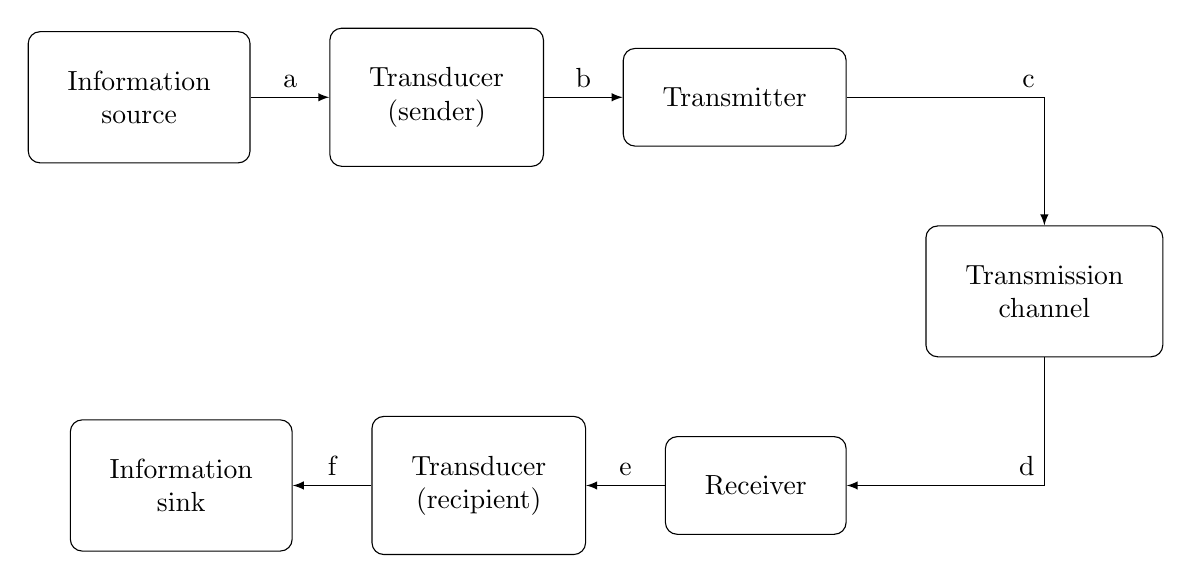
\begin{tikzpicture}
		\draw node[draw, block](Source){Information\\ source};
		\draw node[draw, block, right=of Source](STrans){Transducer\\ (sender)};
		\draw node[draw, block, right=of STrans](TX){Transmitter};
		\draw node[draw, block, below right=of TX](Ch){Transmission\\ channel};
		\draw node[draw, block, below left=of Ch](RX){Receiver};
		\draw node[draw, block, left=of RX](RTrans){Transducer\\ (recipient)};
		\draw node[draw, block, left=of RTrans](Sink){Information\\ sink};
		
		\draw[-latex] (Source) -- node[midway, align=center, above]{a} (STrans);
		\draw[-latex] (STrans) -- node[midway, align=center, above]{b} (TX);
		\draw[-latex] (TX) -| node[midway, align=center, above left]{c} (Ch);
		\draw[-latex] (Ch) |- node[midway, align=center, above left]{d} (RX);
		\draw[-latex] (RX) -- node[midway, align=center, above]{e} (RTrans);
		\draw[-latex] (RTrans) -- node[midway, align=center, above]{f} (Sink);
	\end{tikzpicture}
	\caption{Shannon-Weaver model of communication}
	\label{fig:ch01:shannon_weaver_model}
\end{figure}

\begin{description}
	\item[Information source] The information is created here.
	\item[Signal a] The original information is represented in physical form by a signal.
	\item[Transducer (sender)] The \index{Shannon-Weaver model!transducer} transducer converts the signal from one physical form to another.
	\item[Signal b] The signal is in a form which can be processed by the transmitter.
	\item[Transmitter] The information is modulated on a carrier, which can be transmitted through the transmission channel.
	\item[Signal c] The information is modulated on a carrier and can pass through the transmission channel.
	\item[Tansmission channel] The physical system through which the modulated information passes. \index{transmission channels} Transmission channels are noisy and add disturbances to the information.
	\item[Signal d] It is basically the Signal c. However, noise and disturbances have been added.
	\item[Receiver] The receiver extracts the information from the carrier. Information must be reconstructed from the noisy input signal.
	\item[Signal e] The output signal of the receiver.
	\item[Transducer (recipient)] The signal must be converted into a physical form which can be processed by the information sink.
	\item[Signal f] The signal carries the information in a form which can be used by the information sink.
	\item[Information sink] The endpoint of the information. It uses the information to gain knowledge.
\end{description}

\paragraph{Example: Cell phone}

\begin{enumerate}
	\item The information source is the brain.
	\item Electrical impulses and molecules are conveyed by the nerves to the vocal cords (transducer 1). Vocal cords convert the signals to sound.
	\item The sound is converted to an electrical signal by a microphone (transducer 2).
	\item The electrical pulses are modulated on a radio carrier (transmitter).
	\item Radio waves are transmitted over the air (transmission channel).
	\item A noisy signal is received. The receivers demodulates the information from the radio carrier.
	\item The analogue electrical signal is converted into sound by a speaker (transducer 3).
	\item The sound reaches the ear that converts them to electrical pulses (transducer 4).
	\item Electrical impulses and molecules are conveyed by the nerves to the brain (information sink).
\end{enumerate}


\subsection{Classification of Signals}

A \index{signal} signal conveys information in a form that can be processed by components of the communication systems.

\begin{figure}[H]
	\centering
	\begin{tikzpicture}
		\draw node[block](Main){\textbf{Signals carrying}\\ \textbf{information}};
		\draw node[block, below left=of Main](Analogue){Analogue};
		\draw node[block, below right=of Main](Digital){Digital};
		\draw node[block, below left=of Analogue](TimeCont){Time\\ continuous};
		\draw node[block, below right=of Analogue](TimeDis){Time\\ discrete};
		
		\draw [-latex] (Main) -- (Analogue);
		\draw [-latex] (Main) -- (Digital);
		\draw [-latex] (Analogue) -- (TimeCont);
		\draw [-latex] (Analogue) -- (TimeDis);
	\end{tikzpicture}
	\caption{Classification of signals carrying information}
	\label{fig:ch01:signals_classif}
\end{figure}

\paragraph{Analogue signals.}

\index{signal!analogue signal}
\index{signal!value-continuous}
Analogue signals are represented by values out of a continuous range (\emph{value-continuous}). The range can be limited. However, each real value in this range can be taken.

Examples:
\begin{itemize}
	\item Acoustic signals (speech, sound)
	\item Electric signals (voltage, current)
	\item Light signals (microscope, photograph)
\end{itemize}

\index{signal!time-continuous}
\index{signal!time-discrete}
Analogue signals can be time-continuous or time-discrete. \emph{Time-continuity} means that the signal is defined at any real point of time. A \emph{time-discrete} signal is only defined at certain time instances. The number of time instances can be unlimited. However, the signal is not defined between two time points.

\begin{figure}[H]
	\centering
	\begin{adjustbox}{scale=0.8}
		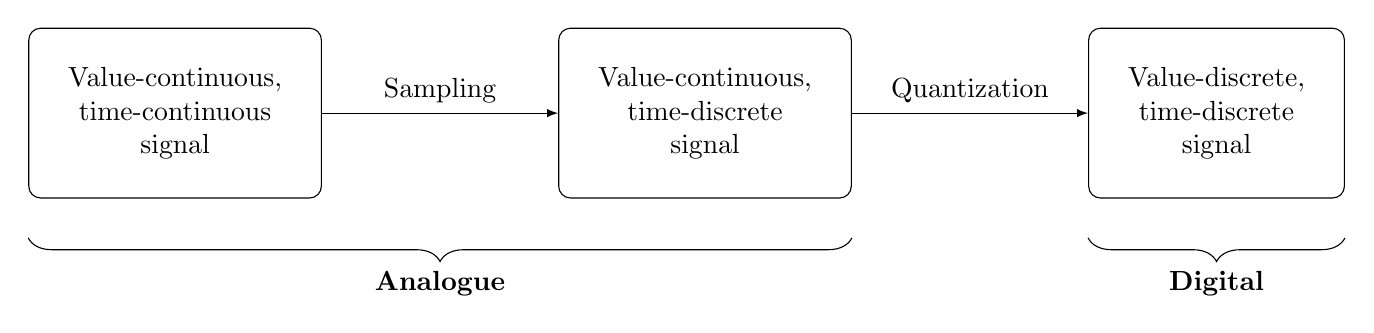
\begin{tikzpicture}
			\draw node[draw, block](Continuous){Value-continuous,\\ time-continuous\\ signal};
			\draw node[draw, block, right=3cm of Continuous](Sampled){Value-continuous,\\ time-discrete\\ signal};
			\draw node[draw, block, right=3cm of Sampled](Digital){Value-discrete,\\ time-discrete\\ signal};
			
			\draw [-latex] (Continuous) -- node[midway, align=center, above]{Sampling} (Sampled);
			\draw [-latex] (Sampled) -- node[midway, align=center, above]{Quantization} (Digital);
			
			\draw[decorate, decoration={brace, amplitude=3mm, mirror}] ([yshift=-5mm] Continuous.south west) -- ([yshift=-5mm] Sampled.south east) node[midway, below, yshift=-3mm]{\textbf{Analogue}};
			\draw[decorate, decoration={brace, amplitude=3mm, mirror}] ([yshift=-5mm] Digital.south west) -- ([yshift=-5mm] Digital.south east) node[midway, below, yshift=-3mm]{\textbf{Digital}};
		\end{tikzpicture}
	\end{adjustbox}
	\caption{Conversion from analogue to digital signals}
	\label{fig:ch01:signals_sampling}
\end{figure}

\begin{figure}[H]
	\centering
	%\includegraphics{../chapter01/Signal_Analogue.jpg}
	\begin{tikzpicture}
		\begin{axis}[
			height={0.25\textheight},
			width=0.6\linewidth,
			scale only axis,
			xlabel={$t$},
			ylabel={$x$},
			%grid style={line width=.6pt, color=lightgray},
			%grid=both,
			grid=none,
			axis lines=left,
			legend pos=north east,
			xmin=0,
			xmax=7,
			ymin=0,
			ymax=3,
			xtick={0, 1, ..., 6},
			ytick={0, 0.5, ..., 2.5}
		]
			\addplot[smooth, blue, thick] coordinates {(0, 1.1) (1, 1.8) (2, 2.1) (3, 1.0) (4, 0.8) (5, 1.7) (6, 2.4)};
		\end{axis}
	\end{tikzpicture}
	\caption[An analogue, value-continuous, time-continuous signal]{An analogue, value-continuous, time-continuous signal. Both time and value can be any real number.}
	\label{fig:ch01:Signal_Analogue}
\end{figure}

\begin{figure}[H]
	\centering
	%\includegraphics{../chapter01/Signal_TimeDiscr.jpg}
	\begin{tikzpicture}
		\begin{axis}[
			height={0.25\textheight},
			width=0.6\linewidth,
			scale only axis,
			xlabel={$t$},
			ylabel={$x$},
			%grid style={line width=.6pt, color=lightgray},
			%grid=both,
			grid=none,
			axis lines=left,
			legend pos=north east,
			xmin=0,
			xmax=7,
			ymin=0,
			ymax=3,
			xtick={0, 1, ..., 6},
			ytick={0, 0.5, ..., 2.5}
		]
			\addplot[smooth, blue, dashed] coordinates {(0, 1.1) (1, 1.8) (2, 2.1) (3, 1.0) (4, 0.8) (5, 1.7) (6, 2.4)};
			\addplot[red, thick] coordinates {(0, 0) (0, 1.1)};
			\addplot[red, thick] coordinates {(1, 0) (1, 1.8)};
			\addplot[red, thick] coordinates {(2, 0) (2, 2.1)};
			\addplot[red, thick] coordinates {(3, 0) (3, 1.0)};
			\addplot[red, thick] coordinates {(4, 0) (4, 0.8)};
			\addplot[red, thick] coordinates {(5, 0) (5, 1.7)};
			\addplot[red, thick] coordinates {(6, 0) (6, 2.4)};
			\addplot[only marks, red, thick, mark=o] coordinates {(0, 1.1) (1, 1.8) (2, 2.1) (3, 1.0) (4, 0.8) (5, 1.7) (6, 2.4)};
		\end{axis}
	\end{tikzpicture}
	\caption[An analogue, value-continuous, but time-discrete signal]{An analogue, value-continuous, but time-discrete signal. Only certain time points (in this case $t \in \mathbb{Z}$) are valid, but the values can be any real number. The red circles form the signal. The vertical lines illustrate that the signal in time-discrete. The blue, dashed signal is not present, but illustrates the original time-continuous signal from which the time-discrete signal has been obtained.}
	\label{fig:ch01:Signal_TimeDiscr}
\end{figure}

\paragraph{Digital signals.}

\index{signal!digital signal}
\index{signal!value-discrete}
Digital signals are both time-discrete and value-discrete. \emph{Value-discrete} means that they can take only one state out of a limited set of states.

\begin{figure}[H]
	\centering
	%\includegraphics{../chapter01/Signal_Digital.jpg}
	\begin{tikzpicture}
		\begin{axis}[
			height={0.25\textheight},
			width=0.6\linewidth,
			scale only axis,
			xlabel={$t$},
			ylabel={$x$},
			%grid style={line width=.6pt, color=lightgray},
			%grid=both,
			xmajorgrids=false,
			ymajorgrids=true,
			grid style={color=lightgray, dashed},
			axis lines=left,
			legend pos=north east,
			xmin=0,
			xmax=7,
			ymin=0,
			ymax=3,
			xtick={0, 1, ..., 6},
			ytick={0, 0.5, ..., 2.5}
		]
			\addplot[smooth, blue, dashed] coordinates {(0, 1.1) (1, 1.8) (2, 2.1) (3, 1.0) (4, 0.8) (5, 1.7) (6, 2.4)};
			\addplot[red, thick] coordinates {(0, 0) (0, 1.0)};
			\addplot[red, thick] coordinates {(1, 0) (1, 2.0)};
			\addplot[red, thick] coordinates {(2, 0) (2, 2.0)};
			\addplot[red, thick] coordinates {(3, 0) (3, 1.0)};
			\addplot[red, thick] coordinates {(4, 0) (4, 1.0)};
			\addplot[red, thick] coordinates {(5, 0) (5, 1.5)};
			\addplot[red, thick] coordinates {(6, 0) (6, 2.5)};
			\addplot[only marks, red, thick, mark=o] coordinates {(0, 1.0) (1, 2.0) (2, 2.0) (3, 1.0) (4, 1.0) (5, 1.5) (6, 2.5)};
		\end{axis}
	\end{tikzpicture}
	\caption[A digital, value-discrete, time-discrete signal]{A digital, value-discrete, time-discrete signal. Only certain time points and a limited set of values (in this case multiples of $0.5$) are valid.}
	\label{fig:ch01:Signal_Digital}
\end{figure}

Examples:
\begin{itemize}
	\item Text letters
	\item Morse code
	\item Coded data
\end{itemize}

\index{signal!binary signal}
A special kind of digital signal is the \textbf{binary signal}. It has two discrete states.

\begin{excursus}{How analogue are digital signals?}
	In fact, the physical form of a digital signal is again an analogue signal. If digital electronics are implemented, digital signals are transferred into a physical form. A binary signal can take the discrete states ``high'' and ``low''. Being on a wire, its states are represented by voltage levels, for example \SI{0}{V} and \SI{3.3}{V}. At this point, the engineer must carefully consider the effects which the signal is subject to. This topic is covered by the field of microwave engineering and \ac{EMC}.
	
	However, if processed by a digital system, the physical representation is of minor importance. The theoretical consideration of digital signals neglects the physical nature. Even more, it is irrelevant which physical form of the digital signal exists and whether it exits. Only the discrete, logical states are of interest.
\end{excursus}


\subsection{Transmission Channels}

\index{transmission channel}
Digital communication systems employ electromagnetic waves to convey information. Therefore, only transmission channels transporting electromagnetic waves are considered.

\begin{figure}[H]
	\centering
	\begin{tikzpicture}
	\draw node[block](Main){\textbf{Transmission}\\ \textbf{channels}};
	\draw node[block, below left=of Main](Wired){Wired\\ channels};
	\draw node[block, below right=of Main](Wireless){Wireless\\ channels};
	
	\draw [-latex] (Main) -- (Wired);
	\draw [-latex] (Main) -- (Wireless);
	\end{tikzpicture}
	\caption{Classification of transmission channels}
	\label{fig:ch01:trans_ch_classif}
\end{figure}

\paragraph{Wired Channels.}

The electromagnetic wave propagates along a transmission line.

Examples of transmission lines:
\begin{itemize}
	\item Cables
	\begin{itemize}
		\item Two wire, twisted-pair \index{twisted-pair cable}
		\item Coaxial cable \index{coaxial cable}
	\end{itemize}
	\item Waveguides \index{waveguide}
	\item Planar lines (on printed circuit boards or integrated circuits)
	\begin{itemize}
		\item Microstrip \index{microstrip}
		\item Coplanar waveguide \index{coplanar waveguide}
	\end{itemize}
	\item Glass fibre (light is an electromagnetic wave, too)
\end{itemize}

\paragraph{Wireless Channels.}

The electromagnetic wave is not bound to a transmission line. It propagates through the space. A medium is not necessary. Electromagnetic wave can also travel through vacuum.

\section{The Electromagnetic Spectrum}

The carrier of information in an electronic communication system are electromagnetic waves -- either bound to a transmission line or wireless. Electromagnetic waves are electric fields $\underline{E}$ and magnetic fields $\underline{H}$, which oscillate at high frequencies.

\begin{excursus}{Maxwell's equations and wave equations}
	The Maxwell's equations are a set of coupled partial differential equations. They are the foundation of classical electromagnetism and classical optics.
	
	\textbf{Gauss' law:}
	\begin{equation}
		\nabla \cdot \cmplxvect{E} = \frac{\rho}{\varepsilon_0}
	\end{equation}
	
	\textbf{Gauss' law of magnetism:}
	\begin{equation}
		\nabla \cdot \cmplxvect{B} = 0
	\end{equation}
	
	\textbf{Faraday's law (electromagnetic induction):}
	\begin{equation}
		\nabla \times \cmplxvect{E} = - \frac{\partial \cmplxvect{B}}{\partial t}
	\end{equation}
	
	\textbf{Ampere's circuital law with Maxwell's extension:}
	\begin{equation}
		\nabla \times \cmplxvect{B} = \mu_0 \left(\cmplxvect{J} + \varepsilon_0 \frac{\partial \cmplxvect{E}}{\partial t} \right)
	\end{equation}
	
	James Clerk Maxwell postulated electromagnetic waves in 1865 \cite{Maxwell1864}. By ``decoupling'' the Maxwell's equations, the wave equations can be isolated for both the electric field and the magnetic field. They describe the wave propagation in any media.
	\begin{subequations}
		\begin{align}
			\Delta \cmplxvect{E} - \underline{\gamma}^2 \cmplxvect{E} &= \vect{0} \\
			\Delta \cmplxvect{H} - \underline{\gamma}^2 \cmplxvect{H} &= \vect{0}
		\end{align}
	\end{subequations}
	where $\underline{\gamma}$ is the complex propagation constant, that devolves into the attenuation constant $\alpha$ and the phase constant $\beta$. $\alpha$ expresses the decrease of the field amplitudes while the wave travels through a lossy medium. $\beta$ determines the propagation speed and the wavelength $\lambda = 2 \pi / \beta$.
	\begin{equation}
		\underline{\gamma} = \alpha + \mathsf{j} \beta
	\end{equation}
\end{excursus}

\begin{figure}[H]
	\centering
	\includegraphics[width=0.8\linewidth]{svg/ch01_EM_Spectrum_Properties.pdf}
	\caption{Diagram of the electromagnetic spectrum. \licensequote{\cite{Inductiveload2007}}{''Inductiveload''}{\href{https://creativecommons.org/licenses/by-sa/3.0/deed.en}{CC-BY-SA 3.0}}}
\end{figure}

Electromagnetic waves have different properties and applications, depending on the frequency. The most interesting range for communication is from radio waves to visible light.
\begin{itemize}
	\item Infrared and visible light are used in glass fibre (optical) communication systems. Before the appearance of electronic communication, light was an important information carrier (lighthouses, optical telegraphs, etc.).
	\item Radio waves and microwaves can be generated by electronics and are radiated by antennas. They have advantages over light like a wider range or their ability to penetrate walls.
\end{itemize}

Instead of the frequency, the \index{wavelength} \textbf{wavelength} $\lambda$ can be given. It is inverse proportional to the frequency with the proportionality constant $c_0$, the speed of light. The wavelength is the distance in which one period of the oscillating electromagnetic wave fits. The higher the frequency, the short the distance which a wave travels until the next period starts.
\begin{equation}
	\lambda = \frac{c_0}{f} = \frac{2 \pi c_0}{\omega}
\end{equation}

\begin{figure}[H]
	\centering
	\includegraphics[width=0.5\linewidth]{svg/ch01_Electromagnetic-Spectrum.pdf}
	\caption{Zooming into the radio spectrum as apart of the electromagnetic spectrum. \licensequote{\cite{Penubag2012}}{"Penubag" and Victor Blacus}{\href{https://creativecommons.org/licenses/by-sa/3.0/deed.en}{CC-BY-SA 3.0}}}
\end{figure}

Radio waves are used as a information carrier since the beginning of the 20th century. They can be further divided in accordance with their properties. The radio spectrum is split into \index{band} \textbf{bands}.

\renewcommand{\arraystretch}{1.5}
\begin{table}[H]
	\centering
	\caption[ITU radio band plan]{\ac{ITU} radio band plan}
	\begin{tabular}{|l|l|l|l|}
		\hline
		Band & Frequency & Properties & Example Applications \\
		\hline
		\hline
		\acs{ELF} & \SIrange{3}{30}{Hz} & \multirow{3}{*}{\begin{minipage}{0.25\textwidth}can penetrate water,\\ follows earth curvature\end{minipage}} & \multirow{3}{*}{\begin{minipage}{0.25\textwidth}submarine communication\end{minipage}} \\
		\cline{1-2}
		\acs{SLF} & \SIrange{30}{300}{Hz} &  &  \\
		\cline{1-2}
		\acs{ULF} & \SIrange{300}{3000}{Hz} &  &  \\
		\cline{1-4}
		\acs{VLF} & \SIrange{3}{30}{kHz} & \multirow{3}{*}{\begin{minipage}{0.25\textwidth}follows earth curvature\end{minipage}} & \begin{minipage}{0.25\textwidth}time signals, geophysics\end{minipage} \\[1.5em]
		\cline{1-2}
		\cline{4-4}
		\acs{LF} & \SIrange{30}{300}{kHz} &  & \begin{minipage}{0.25\textwidth}time signals, maritime navigation, AM broadcasting\end{minipage} \\[1.5em]
		\cline{1-2}
		\cline{4-4}
		\acs{MF} & \SIrange{300}{3000}{kHz} &  & \begin{minipage}{0.25\textwidth}AM broadcasting, aviation navigation, avalanche beacon\end{minipage} \\[1.5em]
		\cline{1-4}
		\acs{HF} & \SIrange{3}{30}{MHz} & \begin{minipage}{0.25\textwidth}reflections at ionosphere\end{minipage} & \begin{minipage}{0.25\textwidth}AM broadcasting, amateur radio, \acs{RFID}, maritime communication, long-distance aviation communication\end{minipage} \\[1.5em]
		\cline{1-4}
		\acs{VHF} & \SIrange{30}{300}{MHz} & \begin{minipage}{0.25\textwidth}quasi-optical propagation,\\ reflections at ionosphere possible\end{minipage} & \begin{minipage}{0.25\textwidth}FM broadcasting, television broadcasting, maritime and aviation communication, land mobile communication, weather satellites\end{minipage} \\[1.5em]
		\cline{1-4}
		\acs{UHF} & \SIrange{300}{3000}{MHz} & \multirow{3}{*}{\begin{minipage}{0.25\textwidth}quasi-optical propagation,\\ higher frequencies generally mean higher attenuation and shorter ranges\end{minipage}} & \begin{minipage}{0.25\textwidth}television broadcasting, \acs{WLAN}, \acs{GPS}, communication satellites, cell phones\end{minipage} \\[1.5em]
		\cline{1-2}
		\cline{4-4}
		\acs{SHF} & \SIrange{3}{30}{GHz} &  & \begin{minipage}{0.25\textwidth}radio astronomy, communication satellites, radar, satellite television broadcasting\end{minipage} \\[1.5em]
		\cline{1-2}
		\cline{4-4}
		\acs{EHF} & \SIrange{30}{300}{GHz} &  & \begin{minipage}{0.25\textwidth}new \acs{WLAN} standard (IEEE\,802.11ad), radar, radio astronomy, imaging (millimeter wave scanners), remote sensing\end{minipage} \\[1.5em]
		\hline
	\end{tabular}
\end{table}

Especially, the bands LF to UHF have been traditionally used in wireless communication. Furthermore, their usage is not limited to wireless systems. For example, cable television uses parts of the VHF or UHF spectra. Cable internet shares the wire with TV broadcasting.

Because of the increasing number of services and growing demands regarding bandwidth and response time, modern communication system advance in the direction of microwaves. The microwave spectrum begins at \SI{3}{GHz}.
%There are dedicate band plans for microwave applications. Table \ref{tab:ch01:IEEE_radar_bands} IEEE radar bands.

%\begin{table}[H]
%	\centering
%	\caption{IEEE radar bands}
%	\label{tab:ch01:IEEE_radar_bands}
%	\begin{tabular}{|l|}
%		\hline
%		Abbreviation \\
%		\hline
%		\hline
%		HF \\
%		\hline
%	\end{tabular}
%\end{table}

The services using the electromagnetic spectrum receive a \index{frequency allocation} \textbf{frequency allocation}. Usually, a national telecommunication regulation authority is responsible for allocation frequencies to the services. They follow recommendations of the \ac{ITU}, a special agency of the \ac{UN}. In Germany, the regulation authority is the Federal Network Agency (Bundesnetzagentur).

\section{Computer Networks}


This course focuses on the technologies which convey information between endpoints, using electromagnetic waves. The information, being conveyed, are called \textbf{data}. The handling of the data is a subject of computer science, especially \emph{computer networks} \index{computer network}. Since data processing is a part of digital communication systems, too, this digression shall give an overview about the employed concepts.


\subsection{Protocols}

Modern communication systems convey information world-wide. These communication links are established over myriads of devices, which form a network. The biggest computer network is the internet.

In order to interact, the devices are required to follow certain rules, which are called \textbf{communication protocols} \index{communication protocol}. Protocols define
\begin{itemize}
	\item the structure and semantics of data,
	\item synchronization of communication, and
	\item possible error recovery methods.
\end{itemize}

Protocols are standardized and must be implemented in every device, which interacts with other devices. Important standardization organizations are amongst others:
\begin{itemize}
	\item The non-profit organization \textbf{\acf{IETF}} issues standards concerning the internet. The standards are called \emph{Request For Comment} (RFC) and are available for everyone for free. Example standards: \ac{IP}, \ac{HTTP}
	\item The \textbf{\acf{IEEE}} has standards committees which develop and publish standards. With respect to the internet, the IEEE\,802 LAN/MAN Standards Committee is the most important one. Example standards: IEEE\,802.11 (\ac{WLAN}, Wifi)
	\item The \textbf{\acf{ETSI}} is an independent, non-profit standardization organization. It is recognized by the European Council and officially responsible for standardization of information and communication technologies in Europe. Example standards: 3G (cell phone system), 4G (cell phone system), TETRA (professional mobile radio system)
\end{itemize}


\subsection{\acs{OSI} Model}

There are many task which a digital communication systems must accomplish.
\begin{itemize}
	\item An application processes user input and displays data to the user.
	\item The application data must be reliably transferred over a network with many nodes.
	\item The network is shared with other users and applications.
	\item The network consists of many links using different physical transmission channels, for example, wired and wireless.
\end{itemize}
For each task, there are communication protocols to solve it. Communication protocols are grouped by the task which they fulfil. There is an increasing level of abstraction from the physical link to the application data. The \index{OSI model} \textbf{\acs{OSI} Model} (Figure \ref{fig:ch01:osi_model}) defines a layer structure for classifying communication protocols, which regards the level of abstraction.

\begin{figure}[H]
	\centering
	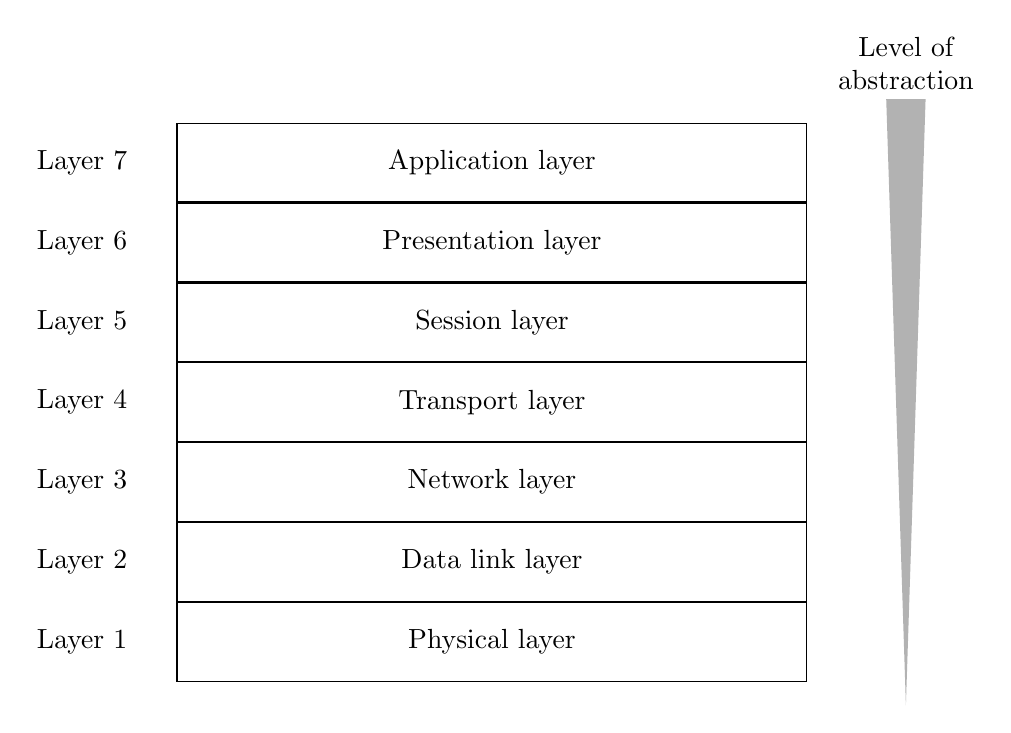
\begin{tikzpicture}[
		layer/.style={
			rectangle,
			minimum height=1cm,
			minimum width=8cm
		}
	]
		\draw node[draw, layer](L7){Application layer};
		\draw node[draw, layer, below=0 of L7](L6){Presentation layer};
		\draw node[draw, layer, below=0 of L6](L5){Session layer};
		\draw node[draw, layer, below=0 of L5](L4){Transport layer};
		\draw node[draw, layer, below=0 of L4](L3){Network layer};
		\draw node[draw, layer, below=0 of L3](L2){Data link layer};
		\draw node[draw, layer, below=0 of L2](L1){Physical layer};
		
		\node [anchor=east, align=right] at([xshift=-5mm] L7.west) {Layer 7};
		\node [anchor=east, align=right] at([xshift=-5mm] L6.west) {Layer 6};
		\node [anchor=east, align=right] at([xshift=-5mm] L5.west) {Layer 5};
		\node [anchor=east, align=right] at([xshift=-5mm] L4.west) {Layer 4};
		\node [anchor=east, align=right] at([xshift=-5mm] L3.west) {Layer 3};
		\node [anchor=east, align=right] at([xshift=-5mm] L2.west) {Layer 2};
		\node [anchor=east, align=right] at([xshift=-5mm] L1.west) {Layer 1};
		
		\filldraw[fill=gray!60, draw=none] ([xshift=10mm, yshift=3mm] L7.north east) -- node[midway, above, anchor=south, align=center]{Level of\\ abstraction} ([xshift=15mm, yshift=3mm] L7.north east) -- ([xshift=12.5mm, yshift=-3mm] L1.south east);
	\end{tikzpicture}
	\caption[OSI Model with seven layers]{\ac{OSI} Model with seven layers}
	\label{fig:ch01:osi_model}
\end{figure}

\begin{table}[H]
	\caption[Description of the layers of the OSI Model]{Description of the layers of the \ac{OSI} Model (Figure \ref{fig:ch01:osi_model}). The protocol data unit is the information }
	\begin{tabular}{|l|l|p{0.5\linewidth}|}
		\hline
		Layer & PDU & Function \\
		\hline
		\hline
		7: Application & Data & Processing user inputs, displaying data, providing services \\
		\hline
		6: Presentation & Data & Translation between network service and application (encryption, compression, etc.) \\
		\hline
		5: Session & Data & Managing sessions (retaining the communication state across multiple contacts) \\
		\hline
		4: Transport & Datagram, Segment & Reliable communication (segmentation, multiplexing, data loss detection) \\
		\hline
		3: Network & Packet & Data transfer across multiple nodes (addressing, routing, traffic control) \\
		\hline
		2: Data link & Frame & Transmission between two devices (medium access, flow control) \\
		\hline
		1: Physical & Symbol & Transmission over a physical medium \\
		\hline
	\end{tabular}
\end{table}

Each protocol has a standardized interface exposed to the upper layer, called \index{service access point} \textbf{\ac{SAP}}. They allow an upper layer protocol to execute functions of the lower layer protocol. These functions are, for example:
\begin{itemize}
	\item Sending or receiving data
	\item Control operations
	\item Network registration and de-registration
\end{itemize}

Protocol layers add own information to the data received from the upper layer. This additional information is required to provide the protocol's functionality. For example, the \acf{IP} needs to add the source and destination address, so that the packet can be routed to the correct endpoint. One can imagine this like data which is written on a letter, which is put into an envelope, which itself is put into another envelope, and so on.

\begin{figure}[H]
	\centering
	\includegraphics{../chapter01/Frame_Wrapping.jpg}
	\caption{Principle of adding more information in each protocol layer}
	\label{fig:ch01:frame_construction}
\end{figure}

Communication protocols may be exchanged in one layer without affecting the functionality of the other layers. For example, \ac{HTTP} operates on \acs{TCP}/\acs{IP}. But the \acf{IP} works on multiple physical links like Ethernet (IEEE\,802.3), Wifi (IEEE\,802.11) or 4G. The transmission media can even change along the communication path. Information travelling through the internet experience lots of \index{media change} \textbf{media changes}. For example, a datagram is firstly sent over a \ac{WLAN} link an relayed by the router on a cable to the internet service provider.


%\begin{figure}[H]
%	\centering
%	\caption{Media change on the internet. }
%	\label{fig:ch01:media_changes}
%\end{figure}

This course on digital communication systems mainly considers the physical layer (layer 1) and the data link layer (layer 2). This physical layer converts the information to physical signals which then leave the device to be transmitted over a physical transmission channel. Networks, which are enabled by protocols of layer 3 and above, are outside the scope of this course.


\subsection{Network Topologies}

In the context of networks,
\begin{itemize}
	\item the devices are called \index{node} \textbf{nodes} and
	\item the communication channels between the nodes are called \index{link} \textbf{links}.
\end{itemize}

Nodes of a network can be arranged in various ways. The structures being formed are \index{network topology} \textbf{network topologies}. Basic topologies are:
\begin{itemize}
	\item \textbf{Line} or chain -- The nodes are connected in series. A packet is passed on by each node until reaches its destination.
	\item \textbf{Ring} -- An extension of the line where the outer nodes are interconnected, too. A packet is passed by every node to its destination. The failure of a single node does not split the network into two segments, which increases the fault tolerance.
	\item \textbf{Bus} -- All nodes are connected to a central cable, the bus. Each node can receive the signals transmitted. As a drawback, only one device may occupy the bus simultaneously for transmission.
	\item \textbf{Star} -- A central node (a hub or switch) relays the packets to its destination.
	\item \textbf{Tree} -- Tree structure is a hybrid network of star networks interconnected by a bus. Because there a no loops in the network, the nodes can be graphically re-ordered to a tree graph.
	\item \textbf{Mesh} -- The nodes are interconnected directly. Nodes may have many direct connections to other nodes, while there is no hierarchy. There are many loops in the network. Usually, mesh networks are re-organized dynamically in mobile systems. A node discovers all nodes which it can reach and establishes a link. A special form is the \emph{Full Mesh}, where all nodes are interconnected with every other one.
\end{itemize}

\begin{figure}[H]
	\centering
	\includegraphics[width=0.7\linewidth]{svg/ch01_NetworkTopologies.pdf}
	\caption{Network topologies. \licensequote{\cite{Maksim2011}}{``Maksim'' and ``Malyszkz''}{Public Domain}}
\end{figure}

The network topology is a concern of the physical and data link layers of the \ac{OSI} model. It can be physical or logical.
\begin{itemize}
	\item The \index{network topology!physical topology} \textbf{physical topology} refers to the placement of the hardware. For example, in a cable network, the physical topology is defined by the cables which interconnect the devices. The topology is mainly implemented in the physical layer.
	\item The \index{network topology!logical topology} \textbf{logical topology} models the data flow in the network. For example, in a wireless network, each node can receive the signals of all other nodes in range. By addressing the devices and filtering out packets with wrong destination addresses, a logical network is created on top of the physical wireless interface. The topology is mainly implemented in the data link layer.
\end{itemize}

A network must fulfil requirements, which determine the network topology, in the end. The use case and constraints must be considered by the engineer. For example:
\begin{itemize}
	\item Lines and trees lack in reliability. The failure of one node divides the network into two segments and the remaining nodes cannot communicate with each other.
	\item The ring is an improvement of the line with respect to reliability. Lines and rings require that all nodes have equal power. Otherwise, the weakest node would be a bottleneck with respect to network bandwidth.
	\item Mesh and fully connected topologies are fault tolerant. The failure of one node does not corrupt the whole network. Furthermore, high data rates and lower latencies may be reached due to a higher number of links.
	\item Mesh and fully connected topologies increase the cost of the networks. Each link consumes energy, space and money.
	\item Buses and stars reduce the cost by maintaining a reasonable amount of reliability. The failure of one device has no major impact on the network, but a disturbance of the bus may. Buses can only be occupied by one node simultaneously. The results in lower data rate and higher latency compared to meshes.
\end{itemize}
An optimal topology may mix the basic forms.

\phantomsection
\addcontentsline{toc}{section}{References}
\printbibliography[heading=subbibliography]
\end{refsection}


\clearpage
% SPDX-License-Identifier: CC-BY-SA-4.0
%
% Copyright (c) 2020 Philipp Le
%
% Except where otherwise noted, this work is licensed under a
% Creative Commons Attribution-ShareAlike 4.0 License.
%
% Please find the full copy of the licence at:
% https://creativecommons.org/licenses/by-sa/4.0/legalcode

\phantomsection
\addcontentsline{toc}{section}{Exercise 1}
\section*{Exercise 1}

\begin{question}[subtitle={Shannon-Weaver Model}]
	Illustrate the process of sending an e-mail using the Shannon-Weaver model! Describe all nodes and edges shortly!
\end{question}

\begin{solution}
	Person A send an e-mail to person B:
	\begin{itemize}
		\item Information source: Brain of person A
		\item Signal: Impulses on nerve cells
		\item Transducer: Keyboard, converts keystrokes to electronic signals
		\item Signal: Electronic signals
		\item Modem: PC, Receives keystrokes and decodes them into the e-mail
		\item Signal: Data
		\item Transmission channel: Internet
		\item Signal: Data
		\item Modem: PC, decodes e-mail, generates text
		\item Signal: Electronic signals
		\item Transducer: Screen, displays text
		\item Signal: Impulses on nerve cells
		\item Information source: Brain of person B
	\end{itemize}
\end{solution}

\begin{question}[subtitle={Classes of Signals}]
	Assign the following signals to the categories: time-continuous vs. time-discrete, value-continuous vs. value-discrete!
	\begin{tasks}
		\task
		$\cos\left(2 \pi \cdot \SI{50}{Hz} \cdot t\right)$
		\task
		Letters: a, B, F, f
		\task
		\begin{equation*}
			f(x) = \begin{cases}
				-1 & \qquad \forall \; x \leq 0 \\
				1 & \qquad \forall \; x > 0
			\end{cases}
		\end{equation*}
	\end{tasks}
\end{question}

\begin{solution}
	\begin{tasks}
		\task
		time-continuous, value-continuous
		\task
		time-discrete, value-discrete
		\task
		time-continuous, value-discrete
	\end{tasks}
\end{solution}

\begin{question}[subtitle={Frequency Allocation}]
	An LTE (4G cell phone) signal can occupy a bandwidth of up to \SI{20}{MHz}. One of the bands allocated to LTE is, amongst others, the band 1 (uplink: \SIrange{1920}{1980}{MHz}, uplink: \SIrange{2110}{2170}{MHz}). The range of one LTE base station is a few kilometres.
	
	However, the HF band (\SIrange{3}{30}{MHz}) has the advantage that waves are reflected by the ionosphere and can propagate over longer distances or even across the whole world. Mostly, narrow-band services like AM broadcasting or amateur radio are allocated to the HF band.
	
	Why is it pointless to use the HF band for LTE?
\end{question}

\begin{solution}
	Reasons:
	\begin{enumerate}
		\item Band capacity:
		\begin{itemize}
			\item HF band is only \SI{27}{MHz} wide.
			\item In contrast, the UHF band is \SI{2700}{MHz} wide.
			\item One LTE base station would occupy the whole HF band.
			\item LTE base stations should only have a limited range. One base station can only service a limited number of users.
			\item Increasing the cell coverage will decrease the number of users and the data rate.
			\item \textbf{That's why high data rate services use higher frequencies.}
		\end{itemize}
		\item Antenna size
		\begin{itemize}
			\item The antenna size is proportional to the wave length. For example, a $\lambda/2$-dipole measures the half of the wave length.
			\item HF band wave length: \SI{10}{100}{m}
			\item UHF band wave length: \SI{0.1}{1}{m}
			\item UHF antennas are much smaller. They must fit into a cell phone.
			\item \textbf{The higher the frequencies, the more compact the antennas and devices.}
		\end{itemize}
	\end{enumerate}
\end{solution}

\begin{question}[subtitle={OSI Layers}]
	What is the difference between a \emph{digital communication system} and a \emph{service}? To which OSI layers are they associated?
\end{question}

\begin{solution}
	\begin{itemize}
		\item Digital communication system (in our understanding): collection of technologies for conveying information
		\item Implemented in lower layers (1 - 4), we consider with layers 1 and 2
		\item Services provide user applications (e.g. video-on-demand, social media, etc.). A service uses communication systems.
		\item Services are located in layer 5 - 7.
	\end{itemize}
\end{solution}

\begin{question}[subtitle={Networks}]
	\begin{tasks}
		\task
		What is the major difference between OSI layers 2 and 3?
		\task
		Give one example for each layer!
		\task
		What is routing?
	\end{tasks}
\end{question}

\begin{solution}
	\begin{tasks}
		\task
		\begin{itemize}
			\item Layer 2: Connection of two devices
			\item Layer 3: Data transfer across multiple nodes (creating a network)
		\end{itemize}
		\task
		\begin{itemize}
			\item Layer 2: IEEE\,802.11 (WiFi)
			\item Layer 3: Internet Protocol (IP)
		\end{itemize}
		\task
		\begin{itemize}
			\item Routing is used in layer 3
			\item A network consists of devices interconnected using layer 2 protocols.
			\item If one device sends a layer 3 packet, it is wrapped into a layer 2 frame and sent to the next node.
			\item The next node unpacks the layer 3 packet.
			\item The next node has to decide to which next node the layer 3 packet should be relayed.
			\item \textbf{This is routing.} Routing means findig the best way to the destination route.
			\item The node packs the layer 3 packet into a layer 2 frame and sends to it the node it has selected.
		\end{itemize}
	\end{tasks}
\end{solution}

\clearpage

\chapter{Time-Continuous Signals and Systems}

\begin{refsection}

All signals considered in this chapter are \index{signal!deterministic signal} \textbf{deterministic}, i.e., its values are predictable at any time. Especially, the values can be calculated by a mathematical equation. In contrast, \emph{random} signals are not predictable. Its values are subject to a random process, which must be modelled stochastically.

Furthermore, the signals considered here are time-continuous.

\index{signal!time-continuous}
\begin{figure}[H]
	\centering
	\begin{tikzpicture}
		\draw node[block](Signals){\textbf{Signal}\\ \textbf{(deterministic)}};
		\draw node[block, below left=of Signals](Periodic){Periodic};
		\draw node[block, below right=of Signals](NonPeriodic){Non-periodic};
		\draw node[block, below left=of Periodic](Mono){Mono-chromatic};
		\draw node[block, below right=of Periodic](Multi){Multi-frequent};
		
		\draw [-latex] (Signals) -- (Periodic);
		\draw [-latex] (Signals) -- (NonPeriodic);
		\draw [-latex] (Periodic) -- (Mono);
		\draw [-latex] (Periodic) -- (Multi);
	\end{tikzpicture}
	\caption{Classification of signals}
	\label{fig:ch02:timecont_signals_classif}
\end{figure}

\section{Mono-Chromatic Signals}

\subsection{Real-Valued Signals and Phasor}

\paragraph{Representation by A Real-Valued Function.}

The mono-chromatic signal $x_{mc}(t)$ is defined by:
\begin{equation}
	x_{mc}(t) = \hat{X} \cdot \cos\left(\omega_0 t - \varphi_0\right)
	\label{eq:ch02:mono_chrom_eq}
\end{equation}
where

\begin{tabular}{ll}
	$\hat{X}$ & is the \index{amplitude} \textbf{amplitude} of the signal, \\
	$\omega_0$ & is the \index{angular frequency} \textbf{angular frequency} of the signal, \\
	$\varphi_0$ & is the \index{phase} \textbf{phase} of the signal, \\
	$t \in \mathbb{R}$ & is the real-value time variable and continuously defined.
\end{tabular}

In fact, the sine function $\sin()$ is mono-chromatic, too. However, it can be derived from \eqref{eq:ch02:mono_chrom_eq} with $\varphi_0 = \SI{90}{\degree}$.

\begin{equation*}
	x_{sin}(t) = \hat{X} \cdot \sin\left(\omega_0 t\right) = \cos\left(\omega_0 t - \SI{90}{\degree}\right)
\end{equation*}

The angular frequency is connected to the \index{frequency} \textbf{frequency}.
\begin{equation}
	\omega_0 = 2 \pi f_0
\end{equation}

\begin{attention}
	You must not confuse the terms \emph{frequency} and \emph{angular frequency}!
\end{attention}

The inverse of the frequency is the \index{period} \textbf{period} $T_0$. It is the time interval at which the signal repeats.
\begin{equation}
	T_0 = \frac{1}{f_0} = \frac{2 \pi}{\omega_0}
\end{equation}

Be aware of the units. The period $T_0$ is defined in seconds \si{s}. The frequency $f_0$ is the inverse of seconds, which is Hertz \si{Hz}. The angular frequency $\omega_0$ is the inverse of seconds, too. However, it is never given in Hertz, only in \si{rad/s} or, more commonly, \si{1/s}.

\begin{table}[H]
	\centering
	\caption{Units}
	\begin{tabular}{|l|l|}
		\hline
		Period $T_0$ & \si{s} \\
		\hline
		Frequency $f_0$ & \si{Hz} \\
		\hline
		Angular frequency $\omega_0$ & \si{1/s} \; (never Hertz!) \\
		\hline
	\end{tabular}
\end{table}

The actual unit of the signal is derived from its amplitude $\hat{X}$ which can be any physical measure.

\paragraph{Representation by A Complex-Valued Phasor.}

A graphical view on the creation of a cosine signal is depicted in Figure \ref{fig:ch02:cos_creation}.

\begin{figure}[H]
	\centering
	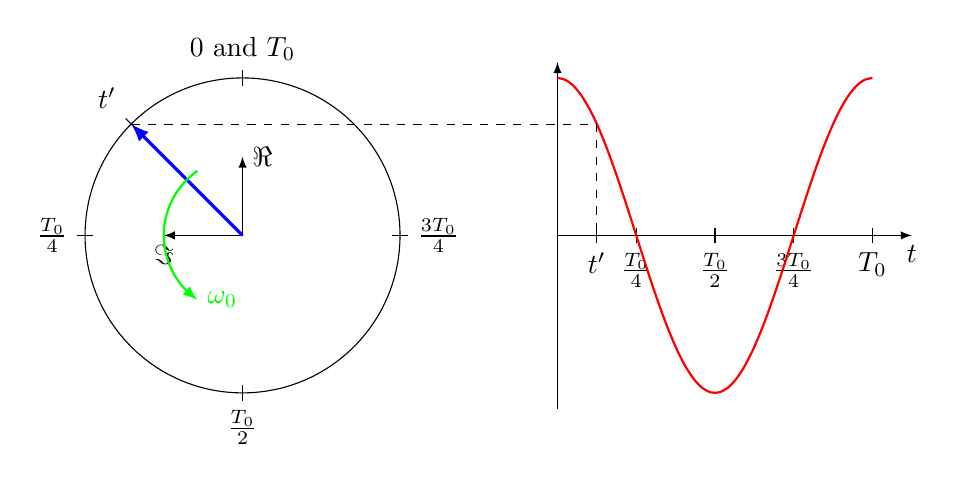
\begin{tikzpicture}
		\begin{scope}[shift={(0, 0)}]
			\draw[-latex] (0,0) -- (4.5,0) node[below, align=left]{$t$};
			\draw[-latex] (0,-2.2) -- (0,2.2);
			\draw (1,0.1) -- (1,-0.1) node[below, align=center]{$\frac{T_0}{4}$};
			\draw (2,0.1) -- (2,-0.1) node[below, align=center]{$\frac{T_0}{2}$};
			\draw (3,0.1) -- (3,-0.1) node[below, align=center]{$\frac{3 T_0}{4}$};
			\draw (4,0.1) -- (4,-0.1) node[below, align=center]{$T_0$};
			
			\draw (0.5,0.1) -- (0.5,-0.1) node[below, align=center]{$t'$};
			
			\draw[red, thick, smooth, domain=0:4, samples=40] plot (\x, {2*cos( 360 * \x / 4 )});
		\end{scope}
		\begin{scope}[shift={(-4, 0)}]
			\draw[draw] (0:2) arc(0:360:2);
			\draw[-latex] (0,0) -- (0,1) node[right, align=left]{$\Re$};
			\draw[-latex] (0,0) -- (-1,0) node[below, align=center]{$\Im$};
			
			\draw (180:1.9) -- (180:2.1) node[left, align=center]{$\frac{T_0}{4}$};
			\draw (270:1.9) -- (270:2.1) node[below, align=center]{$\frac{T_0}{2}$};
			\draw (0:1.9) -- (0:2.1) node[right, align=center]{$\frac{3 T_0}{4}$};
			\draw (90:1.9) -- (90:2.1) node[above, align=center]{$0$ and $T_0$};
			
			\draw (135:1.9) -- (135:2.1) node[above left, align=right]{$t'$};
			
			\draw[very thick, blue, -latex] (135:0) -- (135:2);
			
			
			\draw[thick, green, -latex] (125:1) arc(125:235:1) node[right, align=left]{$\omega_0$};
		\end{scope}
		
		\draw[dashed] (-5.414, 1.414) -- (0.5, 1.414) -- (0.5, 0);
	\end{tikzpicture}
	\caption[Generation of a sinusoidal shape]{Generation of a sinusoidal shape. Imagine, there is a pointer (blue) with one side fixed to a point. Now, it begins rotating counter-clockwise with an angular frequency of $\omega_0$ (green). The arrow of the pointer draws a circle (left side). Each angle of the pointer is related to a time instance. The blue pointer is the current position at time instance $t'$. Its vertical value is projected into the time plot, forming the cosine wave (red).}
	\label{fig:ch02:cos_creation}
\end{figure}

You may now some relations:
\begin{itemize}
	\item A full rotation of the pointer takes exactly one period $T_0$.
	\item The orange cosine curve can be horizontally shifted by redefining the original angle of the pointer at $T_0$. This offset angle is the phase $\varphi_0$.
	\item The length of the pointer and the radius of the circle is the amplitude $\hat{X}$.
\end{itemize}

A mono-chromatic signal can be described by its three parameters
\begin{itemize}
	\item Amplitude $\hat{X}$
	\item Phase $\varphi_0$
	\item Frequency $\omega_0$
\end{itemize}

When a signal passes through a \ac{LTI} system, the amplitude, the phase or both may change. However, the frequency never changes. Thus, the frequency $\omega_0$ is assumed to be constant and neglected. Consequently, the parameters
\begin{itemize}
	\item amplitude $\hat{X}$ and
	\item phase $\varphi_0$
\end{itemize}
remain. Both are absorbed by the complex-valued \index{phasor} \textbf{phasor} $\underline{X}$, which uniquely describes a mono-chromatic signal.
\begin{equation}
	\underline{X} = \hat{X} \cdot e^{-j \varphi_0} = \hat{X} \angle -\varphi_0
\end{equation}

\begin{excursus}{Complex numbers}
	$j$ is the \index{imaginary unit} \textbf{imaginary unit}. It satisfies the equation
	\begin{equation}
		j^2 = -1
	\end{equation}
	There is no real number $j \notin \mathbb{R}$ which satisfies the above solution. $j$ spans the set of complex numbers $\mathbb{C}$.
	
	In mathematics, the imaginary unit is noted as $i$. In engineering context, $j$ is used instead, because $i$ is the symbol of the electric current.
	
	A complex number $\underline{c} \in \mathbb{C}$ can be noted in \index{cartesian form} \textbf{cartesian form}:
	\begin{equation}
		\underline{c} = a + j b
	\end{equation}
	$a \in \mathbb{R}$ is the \index{real part} \textbf{real part} of $\underline{c}$. $b \in \mathbb{R}$ is the \index{imaginary part} \textbf{imaginary part} $\underline{c}$.
	\begin{subequations}
		\begin{align}
			a &= \Re\{\underline{c}\} \\
			b &= \Im\{\underline{c}\}
		\end{align}
	\end{subequations}
	Complex numbers $\underline{c}$ always carry an underline in this lecture to distinguish them from real numbers. However, this is not mandatory.

	Another notation is the \index{polar form} \textbf{polar form}:
	\begin{equation}
		\underline{c} = r \cdot e^{j \varphi}
	\end{equation}
	with
	\begin{subequations}
		\begin{align}
			r &= |\underline{c}| = \sqrt{\Re\{\underline{c}\}^2 + \Im\{\underline{c}\}^2} \\
			\varphi &= \mathrm{atan2} \left(\Im\{\underline{c}\}, \Re\{\underline{c}\}\right) \\
			e^{j \varphi} &= \cos \varphi + j \sin \varphi
		\end{align}
	\end{subequations}
	The polar form can be written in \index{angle notation} \textbf{angle notation}:
	\begin{equation}
		\underline{c} = r \angle \varphi
	\end{equation}
	$r \in \mathbb{R}$ and $\varphi \in \mathbb{R}$ are the \index{polar coordinates} \textbf{polar coordinates}.
\end{excursus}

The phasor $\underline{X} \in \mathbb{C}$ is a complex number, which is mostly represented in polar coordinates (see Figure \ref{fig:ch02:cmplxplane_phasor}).

\begin{figure}[H]
	\centering
	\begin{tikzpicture}
	\draw[->] (-3.2,0) -- (3.2,0) node[below, align=left]{$\Re$};
	\draw[->] (0,-3.2) -- (0,3.2) node[left, align=right]{$\Im$};
	\draw[->, thick] (0, 0) -- (-40:3) node[right, align=left]{Complex phasor $\underline{X}$\\ (position at $t = 0$)};
	\draw (0:1.5) arc(0:-40:1.5) node[midway, right, align=left]{Phase $\varphi_0$};
	
	\draw[->, dashed] (-50:1) arc(-50:30:1) node[right, align=left]{$\omega_0$};
	\end{tikzpicture}
	\caption{Phasor in the complex plane}
	\label{fig:ch02:cmplxplane_phasor}
\end{figure}

Figure \ref{fig:ch02:cmplxplane_phasor} depicts the phasor in the complex plane. Figure \ref{fig:ch02:cos_creation} shows a complex plane, too. Please note that both complex planes are rotated by \SI{90}{\degree} with respect to each other.

\begin{fact}
	The phasor of a signal is a signal parameter, constant and \underline{not} time-dependent.
\end{fact}

The current position of the pointer $\underline{x}(t)$ in the complex plane is obtained by rotating it. It makes a full rotation each $T_0$ periods. Therefore, it rotates at an angular frequency of $\omega_0$. The rotation is a multiplication by $e^{j \omega_0 t}$ in the complex plane. $\underline{x}(t) \in \mathbb{C}$ is a complex value, too.
\begin{equation}
	\underline{x_{mc}}(t) = \underline{X} \cdot e^{j \omega_0 t} = \hat{X} \cdot e^{-j \varphi_0} \cdot e^{j \omega_0 t}
\end{equation}

The real-valued function can be obtained by extracting the real part of the complex-valued current value.
\begin{equation}
	x_{mc}(t) = \Re\left\{\underline{x_{mc}}(t)\right\}
\end{equation}

\begin{proof}{}
	\begin{equation}
		\begin{split}
			x_{mc}(t) &= \Re\left\{\underline{x_{mc}}(t)\right\} \\
			 &= \Re\left\{\hat{X} \cdot e^{-j \varphi_0} \cdot e^{j \omega_0 t}\right\} \\
			 &= \hat{X} \cdot \Re\left\{e^{j \left(\omega_0 t - \varphi_0\right)}\right\} \\
			 &= \hat{X} \cdot \Re\left\{\cos \left(\omega_0 t - \varphi_0\right) + j \sin \left(\omega_0 t - \varphi_0\right)\right\} \\
			 &= \hat{X} \cdot \cos \left(\omega_0 t - \varphi_0\right) \\
		\end{split}
	\end{equation}
\end{proof}

\subsection{Complex-Valued Signals}

\begin{excursus}{Are there complex-valued, mono-chromatic signals?}
	Yes, there is.
	\begin{equation}
		\underline{x}_{mc,e}(t) = \hat{X} \cdot e^{j \left(\omega_0 t - \varphi_0\right)}
	\end{equation}
	is a complex-valued, mono-chromatic signal. We will come back to it later, but not in this chapter.
	
	\vspace{0.5em}
	Phasor representation:
	\begin{equation}
		\underline{x}_{mc,e}(t) = \underline{X} \cdot e^{- j \omega_0 t}
	\end{equation}
	With the phasor $\underline{X}$:
	\begin{equation}
		\underline{X} = \hat{X} \cdot e^{- j \varphi_0} =  \hat{X} \angle -\varphi_0
	\end{equation}
	If you use a phasor, it must be clear from the context, whether you refer to a real-valued or complex-valued, mono-chromatic signal.
\end{excursus}

\section{Periodic Signals and Fourier Series}

Periodic signals $x_p(t)$ comprises a class of signals which indefinitely repeat at constant time intervals $T_0$.
\begin{equation}
	x_p(t + n T_0) = x_p(t) \qquad \forall \; n \in \mathbb{Z}, \quad \mathbb{Z} = \left\{..., -2, -1, 0, 1, 2, ...\right\}
\end{equation}

Mono-chromatic signals are a special kind of periodic signals. Multi-frequent signals are composed a limited or unlimited number of mono-chromatic signals, which superimpose. Multi-frequent signals are periodic signals in general.

\begin{fact}
	Each periodic signal can be decomposed into a superposition of mono-chromatic signals.
\end{fact}

The inverse of the period $T_0$ is $f_0$, which is the \textbf{base frequency}. This is the frequency at the periodic pattern repeats. Again, frequency and angular frequency $\omega_0 = 2 \pi f_0$ must be distinguished.

The periodic signal can now be decomposed in cosine and sine functions with integer multiples of the base frequency $f_0$ or base angular frequency $\omega_0$, respectively. They are called \index{harmonics} \textbf{harmonics}.
\begin{equation}
	\begin{split}
		x_p(t) &= \sum\limits_{n=0}^{\infty} a_n \cos\left(n \omega_0 t\right) + \sum\limits_{m=0}^{\infty} b_m \sin\left(m \omega_0 t\right) \qquad \forall \; n, m \in \mathbb{N} = \left\{0, 1, 2, ...\right\} \\
		 &= a_0 + \sum\limits_{n=1}^{\infty} a_n \cos\left(n \omega_0 t\right) + \sum\limits_{m=1}^{\infty} b_m \sin\left(m \omega_0 t\right) \\
	\end{split}
	\label{eq:ch02:fourier_series}
\end{equation}

What happened to $n = 0$ and $m = 0$? $\cos(0) = 1$ and $\sin(0) = 0$. That's it.

Comparing to the mono-chromatic signals, what happened to the phase $\varphi_0$? The phase $\varphi_0$ is a characteristic of mono-chromatic signals. It is completely absorbed by the coefficients $a_n$ and $b_n$ of the cosine and sine functions.

\subsection{Orthogonality}
\index{orthogonality}
The cosine and sine functions are orthogonal to each other. In geometry, two vectors $\vect{A}$ and $\vect{B}$ are said to be orthogonal, if the angle between them is \SI{90}{\degree}. In this case, their inner product is zero.
\begin{equation}
	\langle \vect{A}, \vect{B} \rangle = 0
\end{equation}

More generally, two functions $f(x)$ and $g(x)$ are orthogonal if their \index{inner product} \textbf{inner product} $\langle f, g \rangle$ is zero. 
\begin{equation}
	0 \stackrel{!}{=} \langle f, g \rangle_w = \int\limits_{a}^{b} f(x) g(x) w(x) \, \mathrm{d} x
\end{equation}
$w(x)$ is a non-negative weight function, which is $w(x) = 1$ in simple cases like this one.

Now, you can prove that the cosine and sine functions are orthogonal to each other.
\begin{equation}
	\int\limits_{-\frac{T_0}{2}}^{\frac{T_0}{2}} \cos\left(n \omega_0 t\right) \sin\left(m \omega_0 t\right) \, \mathrm{d} t = 0 \qquad \forall \; n, m \in \mathbb{Z}
	\label{eq:ch02:orth_rel_cos_sin}
\end{equation}

Furthermore, the sine and cosine functions with \underline{different} indices are orthogonal to each other.
\begin{equation}
	\int\limits_{-\frac{T_0}{2}}^{\frac{T_0}{2}} \cos\left(n \omega_0 t\right) \cos\left(p \omega_0 t\right) \, \mathrm{d} t = \frac{\pi}{\omega_0} \cdot \delta_{np} \qquad \forall \; n, p \in \mathbb{N}
	\label{eq:ch02:orth_rel_cos}
\end{equation}
\begin{equation}
	\int\limits_{-\frac{T_0}{2}}^{\frac{T_0}{2}} \sin\left(m \omega_0 t\right) \sin\left(q \omega_0 t\right) \, \mathrm{d} t = \frac{\pi}{\omega_0} \cdot \delta_{mq} \qquad \forall \; m, q \in \mathbb{N}
	\label{eq:ch02:orth_rel_sin}
\end{equation}
with the Kronecker delta
\begin{equation}
	\delta_{uv} = \begin{cases}
		1 & \qquad \text{if } u = v, \\
		0 & \qquad \text{if } u \neq v
	\end{cases}
	\label{eq:ch02:kronecker_delta}
\end{equation}

The \index{orthogonality relations} \textbf{orthogonality relations} \eqref{eq:ch02:orth_rel_cos_sin}, \eqref{eq:ch02:orth_rel_cos} and \eqref{eq:ch02:orth_rel_sin} point out:
\begin{itemize}
	\item Cosine functions are orthogonal if their indices are different. I.e., $n \neq p$ in \eqref{eq:ch02:orth_rel_cos}.
	\item Sine functions are orthogonal if their indices are different. I.e., $m \neq q$ in \eqref{eq:ch02:orth_rel_sin}.
	\item Cosine and sine function are orthogonal independent of their indices.
	\item The indices are the integer multiples of the base frequency $\omega_0$ (harmonics).
\end{itemize}

\subsection{Extraction of The Coefficients}

The orthogonality relations are useful to extract the coefficients $a_n$ and $b_n$ in \eqref{eq:ch02:fourier_series}. Given is the input signal $\tilde{x}_p(t)$ whose coefficient shall be determined. Following assumptions can be derived from the properties of a periodic signal:
\begin{itemize}
	\item $\tilde{x}_p(t)$ is composed of mono-chromatic cosine and sine functions.
	\item All cosine and sine functions have integer multiples of the base frequency.
	\item Each cosine and sine function has a different weight -- the coefficient.
\end{itemize}

Using the orthogonality relations, the coefficients $\tilde{a}_n$ and $\tilde{b}_n$ can be obtained by:
\begin{subequations}
	\begin{align}
		\tilde{a}_n &= \frac{\omega_0}{\pi} \int\limits_{-\frac{T_0}{2}}^{\frac{T_0}{2}} \tilde{x}_p(t) \cdot \cos\left(n \omega_0 t\right) \, \mathrm{d} t \label{eq_ch02_fourier_series_coeff_an} \\
		\tilde{b}_m &= \frac{\omega_0}{\pi} \int\limits_{-\frac{T_0}{2}}^{\frac{T_0}{2}} \tilde{x}_p(t) \cdot \sin\left(n \omega_0 t\right) \, \mathrm{d} t \label{eq_ch02_fourier_series_coeff_bm}
	\end{align}
\end{subequations}

\begin{proof}{Parameter Extraction for $\tilde{a}_n$}
	Given is a periodic function $\tilde{x}_p(t)$, which can be decomposed into:
	\begin{equation}
		\tilde{x}_p(t) = \sum\limits_{p=0}^{\infty} \tilde{a}_p \cos\left(p \omega_0 t\right) + \sum\limits_{q=0}^{\infty} \tilde{b}_q \sin\left(q \omega_0 t\right)
		\label{eq_ch02_proof_per_sig_example}
	\end{equation}
	The coefficient $\tilde{a}_n$ is of interest.
	
	Inserting \eqref{eq_ch02_proof_per_sig_example} into \eqref{eq_ch02_fourier_series_coeff_an}, yields
	\begin{equation}
		\tilde{a}_n = \frac{\omega_0}{\pi} \int\limits_{-\frac{T_0}{2}}^{\frac{T_0}{2}} \left(\sum\limits_{p=0}^{\infty} \tilde{a}_p \cos\left(p \omega_0 t\right) + \sum\limits_{q=0}^{\infty} \tilde{b}_q \sin\left(q \omega_0 t\right)\right) \cdot \cos\left(n \omega_0 t\right) \, \mathrm{d} t
	\end{equation}
	Due to the orthogonality relations, \underline{all products containing a sine function} and \underline{all products containing a cosine function with the index $n \neq p$} become zero. Furthermore, following must be true: $n = p$
	
	\begin{equation}
		\tilde{a}_n = \tilde{a}_p \frac{\omega_0}{\pi} \int\limits_{-\frac{T_0}{2}}^{\frac{T_0}{2}} \cos\left(p \omega_0 t\right) \cdot \cos\left(n \omega_0 t\right) \, \mathrm{d} t \qquad \text{if } \; n = p
	\end{equation}
	
	Using \eqref{eq:ch02:orth_rel_cos}, the integral resolves to:
	\begin{equation}
		\tilde{a}_n = \tilde{a}_p \frac{\omega_0}{\pi} \frac{\pi}{\omega_0} \qquad \text{if } \; n = p
	\end{equation}
	
	In the end, it could be proven that $\tilde{a}_n = \tilde{a}_p$ for $n = p$.
	
	The proof is analogous for the coefficient $b_n$.
\end{proof}

$\cos\left(n \omega_0 t\right)$ can be seen as a ``test function'', which is used to extract the component with the index $n$. The proof points out:
\begin{itemize}
	\item All sine components are erased by $\cos\left(n \omega_0 t\right)$, due to the orthogonality relations.
	\item All cosine function with index $p \neq n$ are erased by $\cos\left(n \omega_0 t\right)$, due to the orthogonality relations.
\end{itemize}
For $b_m$, $\sin\left(m \omega_0 t\right)$ is analogous.

\begin{excursus}{Illustration of The ``Test Function''}
	For illustration of the ``test functions'', image you have a radio and want to hear a specific station. You tune to the frequency on which the station is broadcasting. All other signals are filtered out, you don't want to hear them. Actually, the radio does not employ orthogonality in this case. However, this illustration might help to understand the meaning of $\cos\left(n \omega_0 t\right)$ and $\sin\left(m \omega_0 t\right)$ \underline{in connection} with the orthogonality relations.
\end{excursus}

A special case is the coefficient $\tilde{a}_0$.
\begin{equation}
	\tilde{a}_0 = \frac{\omega_0}{\pi} \int\limits_{-\frac{T_0}{2}}^{\frac{T_0}{2}} \tilde{x}_p(t) \, \mathrm{d} t
\end{equation}
$\cos\left(n \omega_0 t\right)$ is $1$ for $n = 0$. $\tilde{a}_0$ is the \index{DC offset} \textbf{\ac{DC} offset} of the signal. The above formula is known as the calculation of the signal mean in electrical engineering.

\begin{definition}{Fourier series}
	The composition of a series of mono-chromatic signals as shown in \eqref{eq:ch02:fourier_series} is called \index{Fourier series} \textbf{Fourier series}.
	\begin{equation*}
		x_p(t) = \sum\limits_{n=1}^{\infty} a_n \cos\left(n \omega_0 t\right) + \sum\limits_{m=1}^{\infty} b_m \sin\left(m \omega_0 t\right)
	\end{equation*}
	
	The coefficients can be calculated using \eqref{eq_ch02_fourier_series_coeff_an} and \eqref{eq_ch02_fourier_series_coeff_bm}.
\end{definition}

\subsection{Complex-Valued Fourier Series}

A complex-valued, periodic signal $\underline{x_p}(t)$ can be decomposed into complex-valued mono-chromatic signals. The coefficients $\underline{c}_n$ are phasors.
\begin{equation}
	\underline{x_p}(t) = \sum\limits_{n = -\infty}^{\infty} \underline{c}_n \cdot e^{j n \omega_0 t} \qquad \forall \; n \in \mathbb{Z}
	\label{eq:ch02:fourier_series_cmplx}
\end{equation}

The coefficients $\underline{\tilde{c}}_n$ of an input signal $\underline{\tilde{x}_p}(t)$ can be determined by:
\begin{equation}
	\underline{\tilde{c}}_n = \frac{\omega_0}{2 \pi} \int\limits_{-\frac{T_0}{2}}^{\frac{T_0}{2}} \underline{\tilde{x}_p}(t) \cdot e^{-j n \omega_0 t} \, \mathrm{d} t
	\label{eq_ch02_fourier_series_coeff_cn}
\end{equation}

It is based on the orthogonality relation:
\begin{equation}
	\int\limits_{-\frac{T_0}{2}}^{\frac{T_0}{2}} e^{j n \omega_0 t} e^{-j p \omega_0 t} \, \mathrm{d} t = \frac{2 \pi}{\omega_0} \cdot \delta_{np} \qquad \forall \; n, p \in \mathbb{Z}
	\label{eq:ch02:orth_rel_exp}
\end{equation}

\begin{definition}{Complex-Valued Fourier series}
	A complex-valued, periodic signal $\underline{x_p}(t)$ can be decomposed into a series complex-valued mono-chromatic signals \eqref{eq:ch02:fourier_series_cmplx} -- the \index{Fourier series!complex-valued} \textbf{complex-valued Fourier series}.
	\begin{equation*}
		\underline{x_p}(t) = \sum\limits_{n = -\infty}^{\infty} \underline{c}_n \cdot e^{j n \omega_0 t} \qquad \forall \; n \in \mathbb{Z}
	\end{equation*}
	
	The coefficients can be calculated using \eqref{eq_ch02_fourier_series_coeff_cn}.
\end{definition}

\subsection{Amplitude and Phase Spectra}

Let's consider the complex-valued Fourier series $\underline{x_p}(t)$ \eqref{eq:ch02:fourier_series_cmplx}. The coefficients $\underline{c}_n$ are phasors. Its absolute value (amplitude) $|\underline{c}_n|$ and argument (phase) $\arg\left(\underline{c}_n\right)$ can now be plotted over the index $n$. The index $n \in \mathbb{Z}$ is discrete. Thus, the resulting plots are value-discrete in the dimension of $n$. In contrast, the amplitudes and phases are value-continuous.

\begin{definition}{Spectrum of a period signal}
	\begin{itemize}
		\item The plot of the amplitude $|\underline{c}_n|$ is called \index{amplitude spectrum} \textbf{amplitude spectrum}.
		\item The plot of the phase $\arg\left(\underline{c}_n\right)$ is called \index{phase spectrum} \textbf{phase spectrum}.
		\item When referring to the \index{spectrum} \textbf{spectrum}, generally both amplitude and phase, or their complex-valued representation of $\underline{c}_n$ is meant.
	\end{itemize}
\end{definition}

\begin{fact}
	The index $n \in \mathbb{Z}$ is discrete. The plots of the spectrum are value-discrete in the dimension of $n$.
\end{fact}

When considering a complex-valued signal $\underline{x_p}(t)$, both amplitude and phase can take any value, with following constraints:
\begin{itemize}
	\item The amplitude $|\underline{c}_n|$ is always a positive real number.
	\item The phase $\arg\left(\underline{c}_n\right)$ a real number from the interval $[-\pi, +\pi]$.
\end{itemize}

If the signal $\underline{x_p}(t) = x_p(t)$ is real-valued, i.e., $\Im\left\{\underline{c}_n(t)\right\} = 0$, the values of $\underline{c}_n$ are even more constrained by the \index{spectrum!symmetry rules} \textbf{symmetry rules}:
\begin{itemize}
	\item The coefficients $\underline{c}_n \in \mathbb{C}$ are still complex-valued phasors.
	\item But, the coefficients $\underline{c}_n$ show a special symmetry.
	\begin{itemize}
		\item The amplitude spectrum $|\underline{c}_n|$ is an \underline{even function}. It is symmetric with respect to the $y$-axis.
		\item The phase spectrum $\arg\left(\underline{c}_n\right)$ is an \underline{odd function}. It is symmetric with respect to the origin.
		\item As a consequence, the phase of $\arg\left(\underline{c}_0\right)$ at $n = 0$ must be either $0$ or $\pm \pi$. Note that, $+\pi$ is identical to $-\pi$ in the complex plane. The phase is the sign of the \ac{DC} bias: $\arg\left(\underline{c}_0\right) = 0$ means positive \ac{DC} bias and $\arg\left(\underline{c}_0\right) = \pi$ means negative \ac{DC} bias.
	\end{itemize}
\end{itemize}
These symmetry rules apply for \underline{all} real-valued signals $\underline{x_p}(t) = x_p(t) \in \mathbb{R}$. The symmetry rules ensure that the mono-chromatic components of the Fourier series \eqref{eq:ch02:fourier_series_cmplx} sum up to a real value at each time instance $t \in \mathbb{R}$.

The symmetry rules do \underline{not} apply for complex-valued signals $\underline{x_p}(t) \in \mathbb{C}$.

\begin{figure}[H]
	\centering
	\begin{tikzpicture}
		\begin{axis}[
			height={0.25\textheight},
			width=0.6\linewidth,
			scale only axis,
			xlabel={$n$},
			ylabel={$|\underline{c}_n|$},
			%grid style={line width=.6pt, color=lightgray},
			%grid=both,
			grid=none,
			axis lines=left,
			legend pos=north east,
			xmin=-4,
			xmax=4,
			ymin=0,
			ymax=3,
			xtick={-3, -2, ..., 3},
			ytick={0, 0.5, ..., 2.5},
			axis y line=middle,
			axis x line=middle,
			every axis x label/.style={
				at={(ticklabel* cs:1.05)},
				anchor=north,
			},
			every axis y label/.style={
				at={(ticklabel* cs:1.05)},
				anchor=east,
			}
		]
			\addplot[red, thick] coordinates {(-3, 0) (-3, 2.0)};
			\addplot[red, thick] coordinates {(-2, 0) (-2, 0.4)};
			\addplot[red, thick] coordinates {(-1, 0) (-1, 1.6)};
			\addplot[red, thick] coordinates {(0, 0) (0, 1.1)};
			\addplot[red, thick] coordinates {(1, 0) (1, 1.6)};
			\addplot[red, thick] coordinates {(2, 0) (2, 0.4)};
			\addplot[red, thick] coordinates {(3, 0) (3, 2.0)};
			\addplot[only marks, red, thick, mark=o] coordinates {(-3, 2.0) (-2, 0.4) (-1, 1.6) (0, 1.1) (1, 1.6) (2, 0.4) (3, 2.0)};
		\end{axis}
	\end{tikzpicture}
	\caption[Amplitude Spectrum of a multi-frequent signal]{Amplitude Spectrum of a multi-frequent signal. The absolute values (amplitudes) of the coefficients are plotted. The signal $\underline{c}_n$ is actually real-valued ($\Im\left\{\underline{c}_n(t)\right\} = 0$). This leads a symmetry with respect to the $y$-axis. The amplitude spectrum of a real-valued signal is an even function.}
	\label{fig:ch02:FSeries_Amplitude_Spectrum}
\end{figure}

\begin{figure}[H]
	\centering
	\begin{tikzpicture}
		\begin{axis}[
			height={0.25\textheight},
			width=0.6\linewidth,
			scale only axis,
			xlabel={$n$},
			ylabel={$\arg\left(\underline{c}_n\right)$},
			%grid style={line width=.6pt, color=lightgray},
			%grid=both,
			grid=none,
			axis lines=left,
			legend pos=north east,
			xmin=-4,
			xmax=4,
			ymin=-4,
			ymax=4,
			xtick={-3, -2, ..., 3},
			ytick={-3.14159, -1.5708, 1.5708, 3.14159},
			yticklabels={$-\pi\hspace{0.30cm}$, $-\frac{\pi}{2}$,
$\frac{\pi}{2}$, $\pi\hspace{0.10cm}$},
			axis y line=middle,
			axis x line=middle,
			every axis x label/.style={
				at={(ticklabel* cs:1.05)},
				anchor=north,
			},
			every axis y label/.style={
				at={(ticklabel* cs:1.05)},
				anchor=east,
			}
		]
			\addplot[red, thick] coordinates {(-3, 0) (-3, 3.14159)};
			\addplot[red, thick] coordinates {(-2, 0) (-2, -0.5)};
			\addplot[red, thick] coordinates {(-1, 0) (-1, 1.6)};
			%\addplot[red, thick] coordinates {(0, 0) (0, 0)};
			\addplot[red, thick] coordinates {(1, 0) (1, -1.6)};
			\addplot[red, thick] coordinates {(2, 0) (2, 0.5)};
			\addplot[red, thick] coordinates {(3, 0) (3, -3.14159)};
			\addplot[only marks, red, thick, mark=o] coordinates {(-3, 3.14159) (-2, -0.5) (-1, 1.6) (0, 0.0) (1, -1.6) (2, 0.5) (3, -3.14159)};
			\addplot[only marks, blue, mark=x] coordinates {(0, -3.14159) (0, 0.0) (0, 3.14159)};
		\end{axis}
	\end{tikzpicture}
	\caption[Phase Spectrum of a multi-frequent signal]{Phase Spectrum of a multi-frequent signal. The arguments (phases) of the coefficients are plotted. The signal $\underline{c}_n$ is actually real-valued ($\Im\left\{\underline{c}_n(t)\right\} = 0$). This leads a symmetry with respect to the origin. The phase spectrum of a real-valued signal is an odd function. The blue $x$ define the possible phase values of the coefficient $\underline{c}_0$ of the real-valued signal.}
	\label{fig:ch02:FSeries_Phase_Spectrum}
\end{figure}

\begin{excursus}{Spectra in the nature}
	The spectrum is no abstract, mathematical theory. You can see spectra with your eye:
	\begin{figure}[H]
		\centering
		\includegraphics[scale=1]{../chapter02/Rainbow.jpg}
		\caption[A rainbow showing the spectrum of the sunlight]{A rainbow showing the spectrum of the sunlight: The white sunlight is composed of mono-chromatic, electromagnetic waves of all frequencies which are optically visible for humans. When light passes through a dispersive medium (glass prism, raindrop, etc.), it is refracted. Each mono-chromatic component has a different refraction index. The light components are separated by its frequency and become individually visible. An example, is a rainbow as depicted above. \licensequote{\cite{Arz2007}}{``Arz''}{\href{https://creativecommons.org/licenses/by-sa/3.0/deed.en}{CC-BY-SA 3.0}}}
	\end{figure}
	The rainbow is a natural example of an visible spectrum of the sunlight.
\end{excursus}

\section{Non-Periodic Signals and The Continuous Fourier Transform}

\begin{figure}[H]
	\centering
	\begin{tikzpicture}
		\begin{axis}[
			height={0.25\textheight},
			width=0.6\linewidth,
			scale only axis,
			xlabel={$t$},
			ylabel={$x_{np}(t)$},
			%grid style={line width=.6pt, color=lightgray},
			%grid=both,
			grid=none,
			legend pos=north east,
			axis y line=middle,
			axis x line=middle,
			every axis x label/.style={
				at={(ticklabel* cs:1.05)},
				anchor=north,
			},
			every axis y label/.style={
				at={(ticklabel* cs:1.05)},
				anchor=east,
			},
			xmin=-3,
			xmax=3,
			ymin=0,
			ymax=2,
			xtick={-2, -0.5, ..., 2},
			ytick={0, 0.5, ..., 1.5}
		]
			\addplot[blue, thick] coordinates {(-2, 0) (-0.5, 0)};
			\addplot[blue, dashed] coordinates {(-0.5, 0) (-0.5, 1)};
			\addplot[blue, thick] coordinates {(-0.5, 1) (0.5, 1)};
			\addplot[blue, dashed] coordinates {(0.5, 1) (0.5, 0)};
			\addplot[blue, thick] coordinates {(0.5, 0) (2, 0)};
		\end{axis}
	\end{tikzpicture}
	\caption{The rectangular function $\mathrm{rect}$ as an example for a non-period signal}
	\label{fig:ch02:rect_function}
\end{figure}
\index{rectangular function}

\subsection{Derivation of The Continuous Fourier Transform}

Non-periodic signals have no repeating pattern. Consequently, there is no period $T_0$. Mathematically, the period is indefinite $T_0 \rightarrow \infty$.

A non-periodic signal $\underline{x_{np}}(t)$ cannot be simply decomposed by a Fourier series \eqref{eq:ch02:fourier_series_cmplx}.
\begin{equation}
	\begin{split}
		\underline{x_{np}}(t) &= \lim\limits_{T_0 \rightarrow \infty} \sum\limits_{n = -\infty}^{\infty} \underline{c}_n \cdot e^{j n \omega_0 t} \\
		 &= \lim\limits_{T_0 \rightarrow \infty} \sum\limits_{n = -\infty}^{\infty} \underline{c}_n \cdot e^{j \frac{2 \pi n}{T_0} t}
	\end{split}
	\label{eq:ch02:sig_np_fourier_series}
\end{equation}

The coefficient $\underline{c}_n$ is defined by \eqref{eq_ch02_fourier_series_coeff_cn}:
\begin{equation*}
	\begin{split}
		\underline{c}_n &= \frac{\omega_0}{2 \pi} \int\limits_{t = -\frac{T_0}{2}}^{\frac{T_0}{2}} \underline{x_{np}}(t) \cdot e^{-j n \omega_0 t} \, \mathrm{d} t \\
		 &= \frac{1}{T_0} \int\limits_{t = -\frac{T_0}{2}}^{\frac{T_0}{2}} \underline{x_{np}}(t) \cdot e^{-j n \omega_0 t} \, \mathrm{d} t
	\end{split}
	\label{eq:ch02:sig_np_cn}
\end{equation*}

In this case where $T_0 \rightarrow \infty$, $n \omega_0$ is substituted by the frequency variable $\omega$.
\begin{equation}
	\omega = n \omega_0
	\label{eq:ch02:omega_subst}
\end{equation}

Inserting \eqref{eq:ch02:sig_np_cn} into \eqref{eq:ch02:sig_np_fourier_series} while considering \eqref{eq:ch02:omega_subst}, yields:
\begin{equation}
	\underline{x_{np}}(t) = \lim\limits_{T_0 \rightarrow \infty} \sum\limits_{n = -\infty}^{\infty} \frac{1}{T_0} \left( \int\limits_{t' = -\frac{T_0}{2}}^{\frac{T_0}{2}} \underline{x_{np}}(t') \cdot e^{-j \omega t'} \, \mathrm{d} t' \right) \cdot e^{j \omega t}
\end{equation}
Remember, that $n$ is still in the sum, since it has been absorbed by $\omega = n \omega_0$.

The outer sum is a Rieman sum. $\frac{1}{T_0}$ is substituted by $\frac{\Delta \omega}{2 \pi}$. With $T_0 \rightarrow \infty$, it can be rewritten as an integral.
\begin{equation}
	\underline{x_{np}}(t) = \underbrace{\frac{1}{2 \pi} \int\limits_{\omega = -\infty}^{\infty} \underbrace{\left( \int\limits_{t' = -\infty}^{\infty} \underline{x_{np}}(t') \cdot e^{-j \omega t'} \, \mathrm{d} t' \right)}_{\text{Fourier transform}} \cdot e^{j \omega t} \, \mathrm{d} \omega}_{\text{Inverse Fourier transform}}
\end{equation}

The inner integral is the \textbf{continuous Fourier transform}, also called only \index{Fourier transform} \emph{Fourier transform}. 

\begin{definition}{Fourier Transform}
	The \index{continuous Fourier transform} \textbf{continuous Fourier transform} of the function $\underline{x}(t)$ is:
	\begin{equation}
		\underline{X}(j \omega) = \mathcal{F} \left\{\underline{x}(t)\right\} = \int\limits_{t = -\infty}^{\infty} \underline{x}(t) \cdot e^{-j \omega t} \, \mathrm{d} t
		\label{eq:ch02:def_fourier_transform}
	\end{equation}
	
	The \index{inverse Fourier transform} \index{inverse continuous Fourier transform} \textbf{inverse (continuous) Fourier transform} is:
	\begin{equation}
		\underline{x}(t) = \mathcal{F}^{-1} \left\{\underline{X}(j \omega)\right\} = \frac{1}{2 \pi} \int\limits_{\omega = -\infty}^{\infty} \underline{X}(j \omega) \cdot e^{+j \omega t} \, \mathrm{d} \omega
		\label{eq:ch02:def_inv_fourier_transform}
	\end{equation}
\end{definition}

The Fourier transform $\mathcal{F} \left\{\underline{x}(t)\right\}$ and its inverse $\mathcal{F}^{-1} \left\{\underline{X}(j \omega)\right\}$ both yield functions which depend on $t$ or $\omega$, respectively. This relation is sometimes emphasized by appending $(t)$ or $\left(j \omega\right)$.
\begin{subequations}
	\begin{align}
		\mathcal{F} \left\{\underline{x}(t)\right\} &= \mathcal{F} \left\{\underline{x}(t)\right\} \left(j \omega\right) \\
		\mathcal{F}^{-1} \left\{\underline{X}(j \omega)\right\} &= \mathcal{F}^{-1} \left\{\underline{X}(j \omega)\right\} (t)
	\end{align}
\end{subequations}

\subsection{Amplitude and Phase Spectra}

The value-continuous complex frequency variable $j \omega$ in the continuous Fourier transforms replaced the value-discrete index $n$ of the Fourier series. Due to their similarity, the constraints for all signals and the \index{spectrum!symmetry rules} \textbf{symmetry rules} for real-valued signals apply analogously.

\begin{itemize}
	\item The Fourier transform $\underline{X}(j \omega) \in \mathbb{C}$ is always complex-valued, for both real-valued $\underline{x}(t) = x(t) \in \mathbb{R}$ and complex-valued $\underline{x}(t) \in \mathbb{C}$ signals.
	\item The amplitude $|\underline{X}(j \omega)|$ is always a positive real number.
	\item The phase $\arg\left(\underline{X}(j \omega)\right)$ a real number from the interval $[-\pi, +\pi]$.
	\item For real-valued signals $\underline{x}(t) = x(t) \in \mathbb{R}$, but not for complex-valued $\underline{x}(t) \in \mathbb{C}$ signals, following additional constraints (symmetry rules) apply:
	\begin{itemize}
		\item The amplitude spectrum $|\underline{X}(j \omega)|$ is an \underline{even function}. It is symmetric with respect to the $y$-axis.
		\item The phase spectrum $\arg\left(\underline{X}(j \omega)\right)$ is an \underline{odd function}. It is symmetric with respect to the origin.
		\item As a consequence, the phase of $\arg\left(\underline{X}(0)\right)$ at $j \omega = 0$ must be either $0$ or $\pm \pi$. Note that, $+\pi$ is identical to $-\pi$ in the complex plane. The phase is the sign of the \ac{DC} bias: $\arg\left(\underline{X}(0)\right) = 0$ means positive \ac{DC} bias and $\arg\left(\underline{X}(0)\right) = \pi$ means negative \ac{DC} bias.
	\end{itemize}
\end{itemize}

Let's investigate the \index{rectangular function} rectangular function from Figure \ref{fig:ch02:rect_function}. It is defined as:
\begin{equation}
	\mathrm{rect}(t) = \begin{cases}
		0 & \qquad \text{if } \; |t| > \frac{1}{2}, \\
		1 & \qquad \text{if } \; |t| < \frac{1}{2}
	\end{cases}
	\label{eq:ch02:rect_function}
\end{equation}
The function is undefined for $t = \pm \frac{1}{2}$. The function is now transformed, i.e., $\underline{x}(t) = \mathrm{rect}(t)$.

\begin{equation}
	\underline{X}\left(j \omega\right) =  \int\limits_{t = -\infty}^{\infty} \mathrm{rect}(t) \cdot e^{-j \omega t} \, \mathrm{d} t = \mathrm{sinc}\left(\frac{\omega}{2 \pi}\right)
\end{equation}
where $\mathrm{sinc}(t)$ is the \emph{normalized} sinc function.

\begin{attention}
	Mathematics and engineering use a slightly different definition of the sinc function.
	
	In mathematics, it is \index{sinc function!unnormalized} \textbf{\textit{unnormalized} sinc function}:
	\begin{equation*}
		\mathrm{sinc}(t) = \frac{\sin\left(t\right)}{t}
	\end{equation*}
	
	In the context of signal processing and information theory, it is the \index{sinc function!normalized} \textbf{\textit{normalized} sinc function}:
	\begin{equation*}
		\mathrm{sinc}(t) = \frac{\sin\left(\pi t\right)}{\pi t}
	\end{equation*}
	
	In either case, the value at $t = 0$ is defined to:
	\begin{equation*}
		\mathrm{sinc}(t = 0) = \lim\limits_{t \rightarrow 0} \frac{\sin\left(t\right)}{t} = 1
	\end{equation*}
\end{attention}

The resulting spectra of $\underline{X}\left(j \omega\right)$ can now be drawn. The rectangular function is special. The imaginary part $\Im\left\{\underline{X}\left(j \omega\right)\right\} = 0$ is zero. Thus, the phase can only be $0$ or $\pm \pi$. However, this is a special property of all functions which are real-valued and even in the time domain like the sinc function.

\begin{figure}[H]
	\centering
	\begin{tikzpicture}
		\begin{axis}[
			height={0.25\textheight},
			width=0.6\linewidth,
			scale only axis,
			xlabel={$\omega$},
			ylabel={$|\underline{X}\left(j \omega\right)|$},
			%grid style={line width=.6pt, color=lightgray},
			%grid=both,
			grid=none,
			legend pos=north east,
			axis y line=middle,
			axis x line=middle,
			every axis x label/.style={
				at={(ticklabel* cs:1.05)},
				anchor=north,
			},
			every axis y label/.style={
				at={(ticklabel* cs:1.05)},
				anchor=east,
			},
			xmin=-52,
			xmax=52,
			ymin=0,
			ymax=1.2,
			xtick={-50, -40, ..., 50},
			ytick={0, 0.25, ..., 1.0}
		]
			\addplot[red, thick, smooth, domain=-50:50, samples=200] plot (\x,{abs(sinc((1/(2*pi))*\x))});
		\end{axis}
	\end{tikzpicture}
	\caption{Amplitude spectrum of the rectangular function}
	\label{fig:ch02:rect_function_ampl_spectrum}
\end{figure}

\begin{figure}[H]
	\centering
	\begin{tikzpicture}
		\begin{axis}[
			height={0.25\textheight},
			width=0.6\linewidth,
			scale only axis,
			xlabel={$\omega$},
			ylabel={$\arg\left(\underline{X}(j \omega)\right)$},
			%grid style={line width=.6pt, color=lightgray},
			%grid=both,
			grid=none,
			legend pos=north east,
			axis y line=middle,
			axis x line=middle,
			every axis x label/.style={
				at={(ticklabel* cs:1.05)},
				anchor=north,
			},
			every axis y label/.style={
				at={(ticklabel* cs:1.05)},
				anchor=east,
			},
			xmin=-52,
			xmax=52,
			ymin=-4,
			ymax=4,
			xtick={-50, -40, ..., 50},
			ytick={-3.14159, -1.5708, 1.5708, 3.14159},
			yticklabels={$-\pi\hspace{0.30cm}$, $-\frac{\pi}{2}$,
				$\frac{\pi}{2}$, $\pi\hspace{0.10cm}$},
		]
			\addplot[red, thick] coordinates {(-50, 0) (-39.48, 0)};
			\addplot[red, dashed] coordinates {(-39.48, 0)(-39.48, -3.14159)};
			\addplot[red, thick] coordinates {(-39.48, -3.14159) (-19.74, -3.14159)};
			\addplot[red, dashed] coordinates {(-19.74, -3.14159) (-19.74, 0)};
			\addplot[red, thick] coordinates {(-19.74, 0) (19.74, 0)};
			\addplot[red, dashed] coordinates {(19.74, 0) (19.74, 3.14159)};
			\addplot[red, thick] coordinates {(19.74, 3.14159) (39.48, 3.14159)};
			\addplot[red, dashed] coordinates {(39.48, 3.14159)(39.48, 0)};
			\addplot[red, thick] coordinates {(39.48, 0)(50, 0)};
		\end{axis}
	\end{tikzpicture}
	\caption[Phase spectrum of the rectangular function]{Phase spectrum of the rectangular function. Please note that $- \pi$ is equivalent to $+ \pi$.}
	\label{fig:ch02:rect_function_phase_spectrum}
\end{figure}

\subsection{Time Domain and Frequency Domain}

You have learnt two representations of a signal, so far.
\begin{itemize}
	\item \index{time domain} \textbf{Time domain} -- A signal is a function $\underline{x}(t)$ of the time.
	\item \index{frequency domain} \textbf{Frequency domain} -- A signal is a function $\underline{X}(j \omega)$ of the frequency.
\end{itemize}
Both $\underline{x}(t)$ and $\underline{X}(j \omega)$ refer to the same signal. 

The frequency domain is obtained from the time domain by a transform. For time-continuous signals, these transforms one of:
\begin{itemize}
	\item Fourier series
	\item continuous Fourier transform
\end{itemize}
The time domain is obtained by the respective inverse transform.

\begin{definition}{Transform operator}
	The operation of a transform between time and frequency domain is written as:
	\begin{equation}
		\underline{x}(t) \TransformHoriz \underline{X}(j \omega)
	\end{equation}
	for the transform from time to frequency domain, and vice versa:
	\begin{equation}
		\underline{X}(j \omega) \InversTransformHoriz \underline{x}(t)
	\end{equation}
\end{definition}

\textbf{But what is the purpose of the transforms?}

\begin{figure}[H]
	\centering
	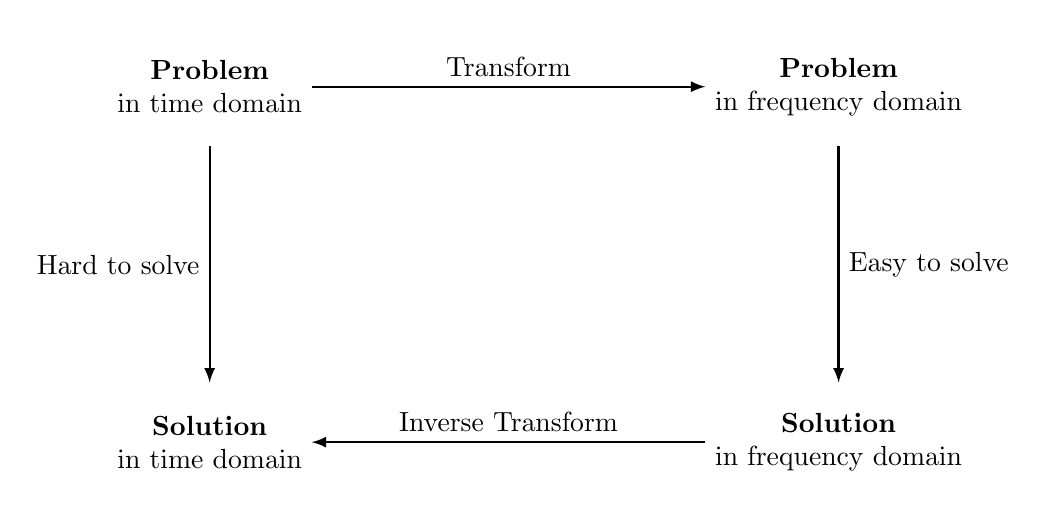
\begin{tikzpicture}
		\node[align=center, minimum width=2.5cm, minimum height=1.5cm] (ProbTD) {\textbf{Problem}\\ in time domain};
		\node[align=center, minimum width=2.5cm, minimum height=1.5cm, right=5cm of ProbTD] (ProbFD) {\textbf{Problem}\\ in frequency domain};
		\node[align=center, minimum width=2.5cm, minimum height=1.5cm, below=3cm of ProbTD] (SolTD) {\textbf{Solution}\\ in time domain};
		\node[align=center, minimum width=2.5cm, minimum height=1.5cm, below=3cm of ProbFD] (SolFD) {\textbf{Solution}\\ in frequency domain};
		
		\draw[-latex, thick] (ProbTD.south) -- node[midway, left, align=right]{Hard to solve} (SolTD.north);
		\draw[-latex, thick] (ProbTD.east) -- node[midway, above, align=center]{Transform} (ProbFD.west);
		\draw[-latex, thick] (ProbFD.south) -- node[midway, right, align=left]{Easy to solve} (SolFD.north);
		\draw[-latex, thick] (SolFD.west) -- node[midway, above, align=center]{Inverse Transform} (SolTD.east);
	\end{tikzpicture}
	\caption{Explanation of the purpose of transforms}
	\label{fig:ch02:benefit_of_transforms}
\end{figure}

\section{Properties of The Continuous Fourier Transform}

\subsection{Energy Signals and Power Signals}

Besides the classification of signals into periodic and non-periodic, signals can be divided into \index{energy signals} \textbf{energy signals} and \index{power signals} \textbf{power signals}.

\begin{definition}{Energy and Power Signals}
	\begin{itemize}
		\item \textbf{Energy signals} have a finite, positive signal energy $0 < E < \infty$, but their average power is zero $P = 0$.
		\item \textbf{Power signals} have a finite, positive average signal power $0 < P < \infty$, but their signal energy is indefinite $E = \infty$.
	\end{itemize}
\end{definition}

The \index{average signal power} \textbf{average signal power} $P$ is a measure for the amount of energy transferred per unit time and defined by:
\begin{equation}
	P = \lim\limits_{T \rightarrow \infty} \frac{1}{T} \int\limits_{-\frac{T}{2}}^{\frac{T}{2}} \left|x(t)\right|^2 \; \mathrm{d} t
\end{equation}
The signal power is connected to the \ac{RMS} value, which is often used in electrical engineering.
\begin{equation}
	\hat{x}_{RMS} = \lim\limits_{T \rightarrow \infty} \sqrt{ \frac{1}{T} \int\limits_{-\frac{T}{2}}^{\frac{T}{2}} \left|x(t)\right|^2 \; \mathrm{d} t}
\end{equation}

The \index{signal energy} \textbf{signal energy} $E$ is:
\begin{equation}
	E = \int\limits_{-\infty}^{\infty} \left|x(t)\right|^2 \; \mathrm{d} t
\end{equation}

The property of power signals, which have an indefinite signal energy, is a problem for the Fourier transform. The transform would yield an indefinite value. Thus:
\begin{fact}
	Every energy signal has a Fourier transform.
\end{fact}

Only some power signals have a Fourier transform. There are distributions which are power signals, but have a Fourier transform, too. Especially, all \emph{tempered distributions} have a Fourier transform.

\subsection{Basic Properties}

All properties of the Fourier transform can be proven using the definition of the Fourier transform \eqref{eq:ch02:def_fourier_transform}.

\subsubsection{Linearity}

Let
\begin{equation}
	\underline{h}(t) = \underline{a} \cdot \underline{f}(t) + \underline{b} \cdot \underline{g}(t)
\end{equation}
where
\begin{itemize}
	\item $\underline{a} \in \mathbb{C}$ and $\underline{b} \in \mathbb{C}$ are complex numbers and
	\item $\underline{f}(t)$ and $\underline{g}(t)$ are Fourier-transformable functions.
\end{itemize}

What is the Fourier transform of $\underline{h}(t)$?
\begin{equation}
	\underline{H}(j \omega) = \mathcal{F} \left\{\underline{h}(t)\right\} = \int\limits_{t = -\infty}^{\infty} \left(\underline{a} \cdot \underline{f}(t) + \underline{b} \cdot \underline{g}(t)\right) \cdot e^{-j \omega t} \, \mathrm{d} t
\end{equation}
The integral can be split into a sum of two integrals.
\begin{equation}
	\underline{H}(j \omega) = \int\limits_{t = -\infty}^{\infty} \underline{a} \cdot \underline{f}(t) \cdot e^{-j \omega t} \, \mathrm{d} t + \int\limits_{t = -\infty}^{\infty} \underline{b} \cdot \underline{g}(t) \cdot e^{-j \omega t} \, \mathrm{d} t
\end{equation}
The constants can be moved in front of the integrals.
\begin{equation}
	\underline{H}(j \omega) = \underline{a} \cdot \underbrace{\int\limits_{t = -\infty}^{\infty} \underline{f}(t) \cdot e^{-j \omega t} \, \mathrm{d} t}_{= \mathcal{F}\left\{\underline{f}(t)\right\}} + \underline{b} \cdot \underbrace{\int\limits_{t = -\infty}^{\infty} \underline{g}(t) \cdot e^{-j \omega t} \, \mathrm{d} t}_{= \mathcal{F}\left\{\underline{g}(t)\right\}}
\end{equation}

\begin{definition}{Linearity of the Fourier transform}
	\begin{equation}
		\mathcal{F}\left\{\underline{a} \cdot \underline{f}(t) + \underline{b} \cdot \underline{g}(t)\right\} = \underline{a} \cdot \mathcal{F}\left\{\underline{f}(t)\right\} + \underline{b} \cdot \mathcal{F}\left\{\underline{g}(t)\right\}
		\label{eq:ch02:op_lin}
	\end{equation}
	where
	\begin{itemize}
		\item $\underline{a} \in \mathbb{C}$ and $\underline{b} \in \mathbb{C}$ are complex numbers and
		\item $\underline{f}(t)$ and $\underline{g}(t)$ are Fourier-transformable functions.
	\end{itemize}
\end{definition}

\subsubsection{Differentiation and Integration}

\begin{definition}{Differentiation of the Fourier transform}
	\begin{equation}
		\mathcal{F}\left\{\frac{\mathrm{d}^n}{\mathrm{d} t^n} \underline{f}(t)\right\} = \left(j \omega\right)^n \underbrace{\underline{F} \left(j \omega\right)}_{= \mathcal{F}\left\{\underline{f}(t)\right\}}
		\label{eq:ch02:op_diff}
	\end{equation}
\end{definition}

\begin{definition}{Integration of the Fourier transform}
	\begin{equation}
		\mathcal{F}\left\{\int\limits_{t'= -\infty}^{t} \underline{f}(t') \, \mathrm{d} t' \right\} = \frac{1}{j \omega} \underbrace{\underline{F} \left(j \omega\right)}_{= \mathcal{F}\left\{\underline{f}(t)\right\}}
		\label{eq:ch02:op_int}
	\end{equation}
\end{definition}

\begin{excursus}{Network analysis of reactive electrical circuits}
	Linear, reactive electrical networks are analysed using the Fourier transform.
	
	For example, voltage and current have following relation in time domain at a capacity:
	\begin{equation}
		u(t) = \frac{1}{C} \int i(t) \, \mathrm{d} t
	\end{equation}
	The expression in complex-valued phasors (frequency domain) is:
	\begin{equation}
		\underline{U} = \underline{Z}_C \cdot \underline{I}
	\end{equation}
	Using the Fourier transform, the impedance $\underline{Z}_C$ can be determined to:
	\begin{equation}
		\underline{Z}_C = \frac{1}{j \omega C}
	\end{equation}
	
	The calculation is analogous for inductances. The volatge-current relation in the time domain is:
	\begin{equation}
		u(t) = L \cdot \frac{\mathrm{d}}{\mathrm{d} t} i(t)
	\end{equation}
	The complex-valued impedance $\underline{Z}_L$ (frequency domain) is:
	\begin{equation}
		\underline{Z}_L = j \omega L
	\end{equation}
\end{excursus}

\subsubsection{Multiplication}

\begin{definition}{Convolution theorem}
	A multiplication in the time-domain becomes a convolution in the frequency domain.
	\begin{equation}
		\mathcal{F}\left\{ \underline{f}(t) \cdot \underline{g}(t) \right\} = \frac{1}{2 \pi} \mathcal{F}\left\{\underline{f}(t)\right\} * \mathcal{F}\left\{\underline{g}(t)\right\}
		\label{eq:ch02:op_mult}
	\end{equation}
\end{definition}

\begin{excursus}{Convolution}
	The convolution is defined to:
	\begin{equation}
		f(t) * g(t) = \left(f * g\right) (t) = \int_{\tau = -\infty}^{\infty} f(\tau) g(t - \tau) \, \mathrm{d} \tau  = \int_{\tau = -\infty}^{t - \infty} f(\tau) g(\tau) \, \mathrm{d} \tau
		\label{eq:ch02:def_convolution}
	\end{equation}
\end{excursus}

\subsubsection{Time Shift}

%Let
%\begin{equation}
%	h(t) = \underline{f}(t - t_0)
%\end{equation}

\begin{definition}{Translation}
	\begin{equation}
		\mathcal{F}\left\{\underline{f}(t - t_0)\right\} = e^{-j t_0 \omega} \cdot \underbrace{\underline{F} \left(j \omega\right)}_{= \mathcal{F}\left\{\underline{f}(t)\right\}}
		\label{eq:ch02:op_time_shift}
	\end{equation}
	where
	\begin{itemize}
		\item $t_0 \in \mathbb{R}$ is a real number and
		\item $\underline{f}(t)$ is a Fourier-transformable function.
	\end{itemize}
\end{definition}

\subsection{Duality}

From \eqref{eq:ch02:def_fourier_transform}, we have:
\begin{equation*}
	\underline{X}(j \omega) = \int\limits_{t = -\infty}^{\infty} \underline{x}(t) \cdot e^{-j \omega t} \, \mathrm{d} t
\end{equation*}
Now, swap $t$ and $-\omega$.
\begin{equation}
	\underline{X}(j t) = - \int\limits_{\omega = \infty}^{-\infty} \underline{x}(-\omega) \cdot e^{j \omega t} \, \mathrm{d} \omega
\end{equation}
Note that:
\begin{itemize}
	\item The negative sign in front of the integral comes from $\mathrm{d} t \rightarrow - \mathrm{d} \omega$
	\item The integration limits $\pm \infty$ are reversed in their sign to $\mp \infty$.
\end{itemize}
Now, extend the right side with $\frac{1}{2 \pi} \cdot 2 \pi$. Let the negative sign be consumed by reversing the integration limits.
\begin{equation}
	\underline{X}(j t) = \frac{1}{2 \pi} \int\limits_{\omega = -\infty}^{\infty} 2 \pi \underline{x}(-\omega) \cdot e^{j \omega t} \, \mathrm{d} \omega
\end{equation}
This equation resembles \eqref{eq:ch02:def_inv_fourier_transform}.
\begin{equation}
	\underline{X}(j t) = \mathcal{F}^{-1} \left\{2 \pi \underline{x}(-\omega)\right\}
\end{equation}

\begin{definition}{Duality}
	Suppose $\underline{g}(t)$ has a Fourier transform $\underline{G}\left(j \omega\right)$, i.e., $\mathcal{F}\left\{\underline{g}(t)\right\} = \underline{G}\left(j \omega\right)$. The Fourier transform of $\underline{G}(t)$ is:
	\begin{equation}
		\mathcal{F}\left\{\underline{G}(j t)\right\} = 2 \pi \cdot \underline{g} \left(-\omega\right)
		\label{eq:ch02:op_duality}
	\end{equation}
	
	The variables $t$ and $\omega$ are swapped in both the original function and its Fourier transform.
\end{definition}

An example for the duality is the convolution in time-domain. Due to the duality, it becomes a multiplication in the frequency domain.
\begin{equation}
	\mathcal{F}\left\{ \underline{f}(t) * \underline{f}(t) \right\} = \mathcal{F}\left\{\underline{f}(t)\right\} \cdot \mathcal{F}\left\{\underline{g}(t)\right\}
	\label{eq:ch02:op_conv}
\end{equation}

\begin{figure}[H]
	\centering
	\begin{tikzpicture}
		\node[align=center, minimum width=2.5cm, minimum height=1.5cm] (TD1) {$\underline{f}(t) \cdot \underline{g}(t)$};
		\node[align=center, minimum width=2.5cm, minimum height=1.5cm, right=3.5cm of TD1] (TD2) {$\underline{f}(t) * \underline{f}(t)$};
		\node[align=center, minimum width=2.5cm, minimum height=1.5cm, below=2cm of TD1] (FD1) {$\frac{1}{2 \pi} \left(\underline{F}\left(j \omega\right) * \underline{G}\left(j \omega\right)\right)$};
		\node[align=center, minimum width=2.5cm, minimum height=1.5cm, below=2cm of TD2] (FD2) {$\underline{F}\left(j \omega\right) \cdot \underline{G}\left(j \omega\right)$};
		
		\node[align=right, anchor=east, left=3cm of TD1] (LabelTD) {\textbf{Time domain}};
		\node[align=right, anchor=east, below=2cm of LabelTD] (LabelFD) {\textbf{Frequency domain}};
		\node[align=right, above=1cm of TD1] (Func1) {\textbf{Function 1}};
		\node[align=right, above=1cm of TD2] (Func2) {\textbf{Function 2}};
		
		%\draw (TD1) node[midway, align=right, rotate=-90]{$\TransformHoriz$} (FD1);
		%\draw (TD2) node[midway, align=right, rotate=-90]{$\TransformHoriz$} (FD2);
		\draw[o-*, thick] (TD1.south) -- (FD1.north);
		\draw[o-*, thick] (TD2.south) -- (FD2.north);
		
		\draw[thick] (TD1.south east) -- (FD2.north west);
		\draw[thick] (TD2.south west) -- (FD1.north east);
	\end{tikzpicture}
	\caption{Duality}
\end{figure}

\paragraph{Consequences of The Duality.}

\begin{itemize}
	\item Uncertainty relationship:
	\begin{itemize}
		\item Signals which are \underline{narrow in time domain} are \underline{wide in frequency domain}.
		\item Signals which are \underline{wide in time domain} are \underline{narrow in frequency domain}.
	\end{itemize}
	\item The duality affects the units of the time variable $t$ and the frequency variable $\omega$.
	\begin{itemize}
		\item The units must be inverse.
		\item If $t$ is in seconds, $\omega$ must be \si{1/s}.
	\end{itemize}
\end{itemize}

\subsection{Dirac Delta Function} \label{sec:ch02_dirac_impulse}

An important distribution is the \index{Dirac delta function} \textbf{Dirac delta function} $\delta(t)$. The Dirac delta function is zero everywhere except at its origin, where it is an indefinitely narrow, indefinitely high pulse.
\begin{equation}
	\delta(t) = \begin{cases}
		+\infty & \qquad \text{if } t = 0, \\
		0 & \qquad \text{if } t \neq 0
	\end{cases}
	\label{eq:ch02:dirac_delta}
\end{equation}
It is constrained by
\begin{equation}
	\int\limits_{-\infty}^{\infty} \delta(t) \; \mathrm{d} t = 1
\end{equation}

\begin{attention}
	The Dirac delta function $\delta(t)$ must not be confused with the Kronecker delta \eqref{eq:ch02:kronecker_delta}. The Dirac delta function operates in continuous space $t \in \mathbb{R}$. The Kronecker delta $\delta_n$ (here one-dimensional) operates in discrete space $n \in \mathbb{Z}$.
\end{attention}

A special feature of the function is called \index{Dirac measure} \textbf{Dirac measure}.
\begin{equation}
	\int\limits_{-\infty}^{\infty} f(t) \delta(t) \; \mathrm{d} t = f(0)
	\label{eq:ch02:dirac_measure}
\end{equation}

Using the Dirac measure, the Fourier transform can be calculated:
\begin{equation}
	\mathcal{F} \left\{\delta(t)\right\} = \int\limits_{-\infty}^{\infty} \delta(t) \cdot e^{-j \omega t} \; \mathrm{d} t = 1
	\label{eq:ch02:ft_dirac}
\end{equation}
The Fourier transform of the Dirac delta function is the frequency-independent constant $1$.

\subsection{Fourier Transforms of Sinusoidal Functions}

\begin{equation}
	\mathcal{F} \left\{\cos\left(\omega_0 t\right)\right\} = \pi \left( \underbrace{\delta\left(\omega - \omega_0\right)}_{\text{Poistive frequency}} + \underbrace{\delta\left(\omega + \omega_0\right)}_{\text{Negative frequency}} \right)
\end{equation}

\begin{equation}
	\mathcal{F} \left\{\sin\left(\omega_0 t\right)\right\} = -j \pi \left( \underbrace{\delta\left(\omega - \omega_0\right)}_{\text{Poistive frequency}} - \underbrace{\delta\left(\omega + \omega_0\right)}_{\text{Negative frequency}} \right)
\end{equation}

\begin{itemize}
	\item The sinusoidal signals (cosine and sine) follow the symmetry rules.
	\begin{itemize}
		\item They have a part in both the positive and the negative frequency half-space (at $- \omega_0$ and $+ \omega_0$).
		\item The cosine function is even.
		\item The sine function is odd.
	\end{itemize}
	\item There are two Dirac delta functions at $- \omega_0$ and $+ \omega_0$.
	\begin{itemize}
		\item The Dirac delta function at $- \omega_0$ or $+ \omega_0$ is $\infty$. Sinusoidal functions are power signals. Remember, they have an infinite energy.
		\item However, the Dirac delta functions can be weighted by the signal amplitude. Linearity of the Fourier transform applies.
		\item Sinusoidal functions are mono-chromatic. So, it makes good sense, that they are only defined at $\pm \omega$.
	\end{itemize}
	\item The Fourier transforms of the cosine and the sine function are phase shifted by $\pi/2$ or \SI{90}{\degree}, respectively, in the complex plane.
	\begin{itemize}
		\item The Fourier transform of the sine function has a $-j$ whilst the cosine function has not.
		\begin{itemize}
			\item $\Im\left\{\mathcal{F} \left\{\cos\left(\omega_0 t\right)\right\}\right\} = 0$ (even function)
			\item $\Re\left\{\mathcal{F} \left\{\sin\left(\omega_0 t\right)\right\}\right\} = 0$ (odd function)
		\end{itemize}
		\item Now, you see the orthogonality of these functions geometrically. ;)
	\end{itemize}
\end{itemize}


\section{\acs{LTI} Systems}

\begin{definition}{System}
	A system is an entity or a process which responds to an input signal with an output signal.
	
	\begin{figure}[H]
		\centering
		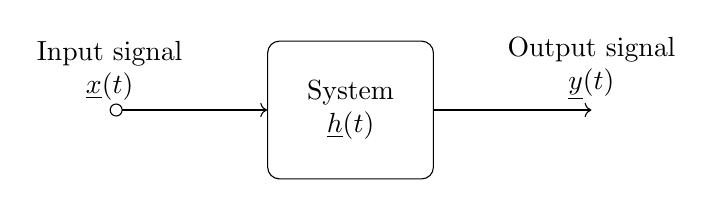
\begin{tikzpicture}
			\node[draw, block] (System) {System\\ $\underline{h}(t)$};
			\draw[<-o] (System.west) -- ++(-2cm, 0) node[above, align=center]{Input signal\\ $\underline{x}(t)$};
			\draw[->] (System.east) -- ++(2cm, 0) node[above, align=center]{Output signal\\ $\underline{y}(t)$};
		\end{tikzpicture}
		\caption{A system with input and output}
	\end{figure}
\end{definition}

\subsection{Classification of Systems}

\begin{description}
	\item[Deterministic or stochastic] A deterministic system is predictable at any time, whereas a stochastic system is based on a random process.
	\item[Causal or non-causal] A system is causal if its output signal $\underline{y}(t_0)$ at the time instance $t_0$ only relies on input signal values of the past, i.e., $\underline{x}(t)$ with $ t \leq t_0$. A is system is non-causal if its output signal also depends on future values of the input signal.
	\item[Linear or non-linear] A linear system fulfils the \textbf{superposition} principle: $y = S(a x_1 + b x_2) = a S(x_1) + b S(x_2)$.
	\item[Time-variant or time-invariant] In a time-invariant system, input signals can be arbitrarily shifted in time, and the system produces an output signal shifted in the same time, i.e., $y(t - \Delta t) = S(x(t - \Delta t))$. In contrast, a system which changes its behaviour over time is time-variant.
	\item[Time-discrete or time-continuous] This is analogous to time-discrete and time-continuous signals.
	\item[One-dimensional or multidimensional] A one-dimensional system has one pair of input and output signals. A multidimensional system processes a vector $\cmplxvect{x}(t)$ of input signals and produces a vector $\cmplxvect{y}(t)$ of output signals.
\end{description}

The focus of this lecture is on \acf{LTI} systems. Systems in this chapter are furthermore deterministic.

\subsection{Transfer Function}

Each deterministic system can be analytically described.

Let's consider an example electrical network with the input voltage $u_i(t)$ and the output voltage $u_o(t)$.
\begin{figure}[H]
	\centering
	\begin{circuitikz}
		\draw (0, 0) to[R, l=$R$, o-] ++(2,0) to[L, l=$L$] ++(2,0) to[short, *-o] ++(2,0);
		\draw (4, 0) to[C, l=$C$, -*] ++(0,-2);
		\draw (0, -2) to[short, o-o] ++(6,0);
		
		\draw (0, 0) to[open, v=$u_i(t)$] (0, -2);
		\draw (6, 0) to[open, v^=$u_o(t)$] (6, -2);
	\end{circuitikz}
	\caption{An example system: a electrical network (2nd order low pass)}
\end{figure}
Using Kirchhoff's circuit laws, the following relation can be determined.
\begin{equation}
	L C \frac{\mathrm{d}^2 u_o(t)}{\mathrm{d} t^2} + R C \frac{\mathrm{d} u_o(t)}{\mathrm{d} t} + u_o(t) = u_e(t)
\end{equation}

It is a second order differential equation. The order corresponds to the number of memories in the system.

Memorizable quantities are for example:
\begin{itemize}
	\item Energy (e.g. in the form of electrical charge, voltage or current)
	\item Information
\end{itemize}
Examples for memories are:
\begin{itemize}
	\item Capacitors (electrical energy)
	\item Inductances (magnetic energy)
	\item Spring (potential energy)
	\item Flip-flop (for digital information)
\end{itemize}

\textbf{How can the output signal of the network $u_o(t)$ determined in relation to a known input signal $u_i(t)$?}

In the time domain, it is hard to solve the differential equation. Remember the explanation of the benefits of transforms (Figure \ref{fig:ch02:benefit_of_transforms}).

Let's use the Fourier transform to formulate a simpler problem.
\begin{equation*}
	L C \frac{\mathrm{d}^2 u_o(t)}{\mathrm{d} t^2} + R C \frac{\mathrm{d} u_o(t)}{\mathrm{d} t} + u_o(t) = u_i(t)
\end{equation*}
is transformed to
\begin{equation}
	\begin{split}
		\left(j \omega\right)^2 L C \underline{U}_o\left(j \omega\right) + \left(j \omega\right) R C \underline{U}_o\left(j \omega\right) + \underline{U}_o\left(j \omega\right) &= \underline{U}_i\left(j \omega\right) \\
		\left(\left(j \omega\right)^2 L C + \left(j \omega\right) R C + 1\right) \underline{U}_o\left(j \omega\right) &= \underline{U}_i\left(j \omega\right) \\
		\left(- \omega^2 L C + j \omega R C + 1\right) \underline{U}_o\left(j \omega\right) &= \underline{U}_i\left(j \omega\right)
	\end{split}
\end{equation}

Now, we can formulate a simple relationship in the frequency domain between the input signal $\underline{U}_i\left(j \omega\right)$ and the output signal $\underline{U}_o\left(j \omega\right)$, which are both now in frequency domain.
\begin{equation}
	\underline{U}_o\left(j \omega\right) = \underline{H} \left(j \omega\right) \cdot \underline{U}_i\left(j \omega\right)
\end{equation}

$\underline{H} \left(j \omega\right)$ is the \index{transfer function} \textbf{transfer function} which fully describes a deterministic \ac{LTI} system.

In our electric network, the transfer function is:
\begin{equation}
	\underline{H} \left(j \omega\right) = \frac{1}{- \omega^2 L C + j \omega R C + 1}
\end{equation}

In general:
\begin{definition}{Transfer function}
	The \index{transfer function} \textbf{transfer function} of a system with the input $\underline{X}\left(j \omega\right) \InversTransformHoriz \underline{x}(t)$ and the output $\underline{Y}\left(j \omega\right) \InversTransformHoriz \underline{y}(t)$ is:
	\begin{equation}
		\underline{H} \left(j \omega\right) = \frac{\underline{Y}\left(j \omega\right)}{\underline{X}\left(j \omega\right)}
		\label{eq:ch02:tranfer_func}
	\end{equation}
\end{definition}

\begin{excursus}{I'm lost! I have a non-linear system.}
	Your are not! Under certain conditions, a non-linear system can be linearized.
	
	Using the \index{Taylor series} \textbf{Taylor series}, a non-linear function can be split into a series of polynomials.
	\begin{equation}
		f(t) = \sum_{n=0}^{\infty} \left. \frac{1}{n!} \frac{\mathrm{d}^n f(t)}{\mathrm{d} t^n} \right|_{t = t_0} \left(t - t_0\right)^n
	\end{equation}
	The Taylor series is developed around a specific \index{operating point} \textbf{operating point} $t_0$.
	
	Using only the polynomials of orders $n = 0$ and $n = 1$, we obtain a linear equation. This procedure is called \index{Taylor approximation} \textbf{Taylor approximation}.
	\begin{equation}
		f(t) \approx f(t_0) + \underbrace{\left. \frac{\mathrm{d} f(t)}{\mathrm{d} t} \right|_{t = t_0}}_{= f'(t_0)} \left(t - t_0\right) \qquad \forall \; |t - t_0| \rightarrow 0
	\end{equation}
	The Taylor approximation using just the polynomials up to $n = 1$ is called \index{linearization} \textbf{linearization}. The approximation is only valid around the operating point $t_0$, i.e., $t$ is constrained $|t - t_0| < \xi$. The approximation gets more imprecise for greater $\xi$.
	
	Linearization is a common method in electronic circuit analysis to model semiconductors, which are always non-linear. Semiconductors are based on an $e$-function.
\end{excursus}


\subsection{Impulse Response}

Let's transfer \eqref{eq:ch02:tranfer_func} back to the time domain.
\begin{equation}
	\underline{y}(t) = \underline{h}(t) * \underline{x}(t)
\end{equation}
The convolution (see \eqref{eq:ch02:def_convolution}) can be resolved to:
\begin{equation}
	\underline{y}(t) = \int_{\tau = -\infty}^{\infty} \underline{h}(\tau) \underline{x}(t - \tau) \, \mathrm{d} \tau = \int_{\tau = -\infty}^{\infty} \underline{h}(t - \tau) \underline{x}(\tau) \, \mathrm{d} \tau
\end{equation}

Now, the input signal is set to the Dirac delta function $\delta(t)$ (see \eqref{eq:ch02:dirac_delta}).
\begin{equation}
	\begin{split}
		\underline{y}_\delta(t) &= \underline{h}(t) * \underline{x}(t) \\
		 &= \int_{\tau = -\infty}^{\infty} \underline{h}(\tau) \delta(t - \tau) \, \mathrm{d} \tau \\
		 &= \underline{h}(t)
	\end{split}
\end{equation}

\begin{itemize}
	\item The convolution can be seen as the Dirac pulse shifted across the time axis and then multiplied by $\underline{h}(t)$ and integrated.
	\item Using the Dirac measure \eqref{eq:ch02:dirac_measure}, the integral becomes zero for all $\tau \neq t$.
	\item The integral becomes $\underline{h}(t)$ for all $\tau = t$.
\end{itemize}

\begin{definition}{Impulse response}
	The inverse Fourier transform of the transfer function $\underline{H} \left(j \omega\right)$ is the \index{impulse response} \textbf{impulse response} $\underline{h}(t)$.
	\begin{equation}
		\underline{h}(t) = \mathcal{F}^{-1}\left\{\underline{H} \left(j \omega\right)\right\}
	\end{equation}
\end{definition}

The name ``impulse response'' directly connected to the Dirac delta function. The Dirac delta function can be seen as an ideal impulse (indefinitely narrow width in time, indefinitely high in value). Giving this impulse as an input into a system yields the impulse response.

\begin{fact}
	The impulse response is the time-domain response of a system to an ideal impulse (Dirac delta function).
\end{fact}

So, theoretically, you can obtain the impulse response -- and thereby a complete definition of the system -- by feeding a Dirac delta function into its input. Of course, this is not possible because a Dirac delta function cannot be generated in nature. However, it can be approximated (e.g. ultra-narrow and high-voltage pulse), yielding the impulse response of the ``system under test'' with uncertainties.

\begin{proof}{}
	A proof in the frequency domain is simple.
	
	Assume that $\underline{x}(t) = \delta(t)$, then $\underline{X}\left(j \omega\right) = 1$ (see \eqref{eq:ch02:ft_dirac}). Using \eqref{eq:ch02:tranfer_func},
	\begin{equation}
		\underline{Y}_\delta\left(j \omega\right) = \underline{H}\left(j \omega\right) \cdot \underbrace{\underline{X}\left(j \omega\right)}_{= 1} = \underline{H}\left(j \omega\right)
	\end{equation}
	
	Transform back to the time domain:
	\begin{equation}
		\underline{y}_\delta(t) = \underline{h}(t)
	\end{equation}
\end{proof}

You have learnt that any deterministic \ac{LTI} system can be expressed by:
\begin{itemize}
	\item transfer function
	\item impulse response
\end{itemize}

\subsection{Causality}

As already described in the introduction to this subsection, a system is causal if it does not rely on future input values.

\begin{definition}{Causality of a system}
	The impulse response of a stable system is constrained by:
	\begin{equation}
		\underline{h}(t) = 0 \qquad \forall \; t < 0
	\end{equation}
\end{definition}

Let's take rectangle function \eqref{eq:ch02:rect_function} as an example for the transfer function of a system:
\begin{equation}
	\underline{H}\left(j \omega\right) = \mathrm{rect}(\omega) = \begin{cases}
		0 & \qquad \text{if } \; |\omega| > \frac{1}{2}, \\
		1 & \qquad \text{if } \; |\omega| < \frac{1}{2}
	\end{cases}
\end{equation}
The inverse Fourier transform is, due to the duality, a sinc-function in time-domain:
\begin{figure}[H]
	\centering
	\begin{tikzpicture}
	\begin{axis}[
		height={0.25\textheight},
		width=0.6\linewidth,
		scale only axis,
		xlabel={$t$},
		ylabel={$|\underline{h}(t)|$},
		%grid style={line width=.6pt, color=lightgray},
		%grid=both,
		grid=none,
		legend pos=north east,
		axis y line=middle,
		axis x line=middle,
		every axis x label/.style={
			at={(ticklabel* cs:1.05)},
			anchor=north,
		},
		every axis y label/.style={
			at={(ticklabel* cs:1.05)},
			anchor=east,
		},
		xmin=-52,
		xmax=52,
		ymin=0,
		ymax=1.2,
		xtick={-50, -40, ..., 50},
		ytick={0, 0.25, ..., 1.0}
	]
		\addplot[blue, thick, smooth, domain=-50:50, samples=200] plot (\x,{abs(sinc((1/(2*pi))*\x))});
		\addlegendentry{Non-causal system impulse response};
		\addplot[red, thick, smooth, domain=0:50, samples=200] plot (\x,{0.5*abs(sinc((1/(2*pi))*\x))});
		\addlegendentry{Causal system impulse response};
	\end{axis}
	\end{tikzpicture}
	\caption{Impulse response of a system with a rectangular function as its transfer function}
\end{figure}
The system's impulse response $\underline{h}(t)$ (blue curve) is also defined in $t < 0$. Therefore, it is non-causal.

If $\underline{h}(t)$ is constrained to be zero for all $t < 0$ (red curve). It would be causal. However, the transfer function $\underline{H}\left(j \omega\right)$ would be different.

\begin{fact}
	Non-causal systems need to reliably predict future values of the input signal. Therefore, it is not possible to implement them in real.
\end{fact}

\subsection{Zeroes and Poles}

\begin{excursus}{Relationship between Fourier transform and Laplace transform}
	The \index{Laplace transform} Laplace transform is another integral transform, which is closely related to the Fourier transform. The (two-sided) Laplace transform is defined by:
	\begin{equation}
		\underline{X}(\underline{s}) = \mathcal{L} \left\{\underline{x}(t)\right\} = \int\limits_{t = -\infty}^{\infty} \underline{x}(t) e^{- \underline{s} t} \, \mathrm{d} t
	\end{equation}
	$\underline{x}(t)$ is the original (time-domain) function. $X(\underline{s})$ is the Laplace transform in frequency domain. $\underline{s}$ is the complex frequency variable, corresponding to $j \omega$ in the Fourier transform. In fact, $\underline{s}$ can be decomposed to:
	\begin{equation}
		\underline{s} = \sigma + j \omega
	\end{equation}
	The frequency variable of the Laplace transform is two-dimensional, whereas the frequency variable of the Fourier transform is one-dimensional.
	
	\begin{figure}[H]
		\centering
		\begin{tikzpicture}
			\draw[->] (-2.2,0) -- (2.2,0) node[below, align=left]{$\Re\left\{\underline{s}\right\}$};
			\draw[->] (0,-2.2) -- (0,2.2) node[left, align=right]{$\Im\left\{\underline{s}\right\}$};
			\draw[thick, red] (0,-2) -- (0,2);
			\draw[dashed, red] (0,1) -- (1,1.2) node[right, align=left, color=red]{$j \omega$};
		\end{tikzpicture}
		\caption{Complex plane of the complex frequency variable $\underline{s}$}
	\end{figure}
	
	The Fourier transform is a special case of the Laplace transform, setting $\sigma = 0$. The complex frequency variable becomes $\underline{s} = j \omega$. In the complex plane, the frequency variable $j \omega$ is only the imaginary axis.
	
	\vspace{0.5em}
	
	\textbf{Why two transforms?} Actually, the Laplace transform fully describes the system, including transients. Fourier transform neglects the transients due to $\sigma = 0$ and expects a \textbf{steady-state}.
	\begin{itemize}
		\item The Laplace transform is used for a full analysis of the system, especially transient analysis. Therefore, it is used in control engineering to describe components of a control system and analyse its stability (zeros and poles).
		\item The Fourier transform is suitable for steady-state analysis of a system. That means, that any on/off switching process has happened far in the past $t \rightarrow -\infty$.
	\end{itemize}
	
	However, in the literature Fourier transform is inconsistently used to analyse the poles and zeros of a system. In fact, a Laplace transform is behind this. But, that is just a notation issue, because $\omega$ is used instead of $\underline{s}$.
	
	The Fourier transform is more common in the field of signal processing and information theory, because signals are mostly steady-state and transients are of minor interest. That's why we stick to it.
\end{excursus}

In system analysis, zeros and poles play an important role.
\begin{itemize}
	\item $\underline{s}_0$ is a zero of the system with the transfer function $\underline{H}(\underline{s})$, when $\underline{H}(\underline{s}_0) = 0$.
	\item $\underline{s}_\infty$ is a pole of the system with the transfer function $\underline{H}(\underline{s})$, when $\underline{H}(\underline{s}_\infty) \rightarrow \pm \infty$.
\end{itemize}

$\underline{H}(\underline{s})$ can be written as a fraction with polynomials in both the numerator and denominator.
\begin{equation}
	\underline{H}(\underline{s}) = \frac{(\underline{s} - \underline{s}_{0,0}) (\underline{s} - \underline{s}_{0,1}) \ldots  (\underline{s} - \underline{s}_{0,p})}{(\underline{s} - \underline{s}_{\infty,0}) (\underline{s} - \underline{s}_{\infty,1}) \ldots (\underline{s} - \underline{s}_{\infty,q})}
\end{equation}
\begin{itemize}
	\item Zeros $\underline{s}_0$ are all values for $\underline{s}$ that make the numerator zero.
	\item Poles $\underline{s}_\infty$ are all values for $\underline{s}$ that make the denominator zero.
	\item There can be multiple zeros and poles with the same value. Counting their number yields their order.
\end{itemize}

Let's investigate the following example:
\begin{equation}
	\underline{H}(\underline{s}) = \frac{\underline{s}^2 - 2 j \underline{s} - 1}{\underline{s}^2 - 4} = \frac{(\underline{s} - j)^2}{(\underline{s} + 2) (\underline{s} - 2)}
\end{equation}
The system has
\begin{itemize}
	\item a zero of 2nd order at $\underline{s}_{0,0} = j$,
	\item a pole of 1st order at $\underline{s}_{\infty,0} = 2$, and
	\item a pole of 1st order at $\underline{s}_{\infty,1} = -2$.
\end{itemize}
\begin{figure}[H]
	\centering
	\begin{tikzpicture}
		\begin{axis}[
			height={0.25\textheight},
			width=0.6\linewidth,
			scale only axis,
			xlabel={$\Re\left\{\underline{s}_\infty\right\} = \sigma$},
			ylabel={$\Im\left\{\underline{s}_\infty\right\} = \omega$},
			%grid style={line width=.6pt, color=lightgray},
			%grid=both,
			grid=none,
			legend pos=north east,
			axis y line=middle,
			axis x line=middle,
			every axis x label/.style={
				at={(ticklabel* cs:1.05)},
				anchor=north,
			},
			every axis y label/.style={
				at={(ticklabel* cs:1.05)},
				anchor=east,
			},
			xmin=-3,
			xmax=3,
			ymin=-3,
			ymax=3,
			xtick={-2, -1, ..., 2},
			ytick={-2, -1, ..., 2},
		]
			\addplot[red, only marks, mark=o] coordinates {(0, 1)};
			\addlegendentry{Zeros};
			\addplot[red, only marks, mark=x] coordinates {(2, 0) (-2, 0)};
			\addlegendentry{Poles};
		\end{axis}
	\end{tikzpicture}
	\caption{Zeros and poles of the example system}
\end{figure}

The zeros and poles are used to analyse the stability of a system.
\begin{itemize}
	\item The input signal $|\underline{x}(t)| < \infty \quad \forall \; t \in \mathbb{R}$ is bounded, i.e. not infinite.
	\item A stable system always emits a output signal $|\underline{x}(t)| < \infty \quad \forall \; t \in \mathbb{R}$ which is bounded, too.
	\item This is called \index{BIBO stability} \textbf{\ac{BIBO} stability}.
	\item To archive \ac{BIBO} stability, all poles must be on the left side of the complex plane including the imaginary axis: $\Re\left\{\underline{s}_\infty\right\} \stackrel{!}{\leq} 0$.
\end{itemize}

\subsection{Amplitude and Phase Response}

The complex transfer function of a system can be decomposed to polar coordinates:
\begin{equation}
	\underline{H}\left(j \omega\right) = A(\omega) \cdot e^{j \varphi(\omega)}
\end{equation}
Both $A(\omega)$ and $\varphi(\omega)$ are functions of the angular frequency $\omega$.

Each input signal $\underline{x}(t) \TransformHoriz \underline{X}\left(j \omega\right)$ is subject to
\begin{itemize}
	\item a change in amplitude, called \emph{gain} or \index{amplitude response} \textbf{amplitude response} $A(\omega)$: $|\underline{Y}\left(j \omega\right)| = A(\omega) \cdot |\underline{X}\left(j \omega\right)|$
	\item a shift in phase, called \emph{phase shift} or \index{phase response} \textbf{phase response} $\varphi(\omega)$: $\arg\left(\underline{Y}\left(j \omega\right)\right) = \varphi(\omega) + \arg\left(\underline{X}\left(j \omega\right)\right)$
\end{itemize}

For each mono-chromatic component of the signal at an angular frequency of $\omega$, the gain and phase shift can be illustrated:
\begin{figure}[H]
	\centering
	\begin{tikzpicture}
		\begin{axis}[
			height={0.25\textheight},
			width=0.6\linewidth,
			scale only axis,
			xlabel={$t$},
			ylabel={$x(t), y(t)$},
			%grid style={line width=.6pt, color=lightgray},
			%grid=both,
			grid=none,
			legend pos=north east,
			axis y line=middle,
			axis x line=middle,
			every axis x label/.style={
				at={(ticklabel* cs:1.05)},
				anchor=north,
			},
			every axis y label/.style={
				at={(ticklabel* cs:1.05)},
				anchor=east,
			},
			xmin=-3,
			xmax=3,
			ymin=-3,
			ymax=3,
			xtick={-2, -1, ..., 2},
			ytick={-2, -1, ..., 2},
		]
			\addplot[blue, domain=-2:2, samples=100] plot (\x, {2*sin(360*\x)});
			\addlegendentry{$x(t)$};
			\addplot[red, domain=-2:2, samples=100] plot (\x, {sin((360*\x - 45)});
			\addlegendentry{$y(t)$};
		\end{axis}
	\end{tikzpicture}
	\caption[Gain and phase shift of a mono-chromatic signal]{Gain and phase shift of a mono-chromatic signal. Here, the gain $A = 0.5$ and the phase shift is $\varphi = \frac{\pi}{4} = \SI{45}{\degree}$.}
	\label{fig:ch02:gain_phase_shift}
\end{figure}

\textit{Remarks:}
\begin{itemize}
	\item The system does never change the frequency of a mono-chromatic signal, because the system is linear.
	\item The envelope (shape of the signal) of a multi-frequent signals may however be altered. Each mono-chromatic component is subject to its own change by $\underline{H}\left(j \omega\right)$.
\end{itemize}

The values of both the amplitude response $A(\omega)$ and the phase response $\varphi(\omega)$ can be plotted over the angular frequency $\omega$.

Let's take an example:
\begin{equation}
	\underline{H}\left(j \omega\right) = \frac{3}{j \omega \tau + 1}
\end{equation}
with $\tau = \SI{0.05}{s}$.

\begin{figure}[H]
	\centering
	\begin{tikzpicture}
		\begin{axis}[
			height={0.25\textheight},
			width=0.8\linewidth,
			scale only axis,
			xlabel={$\omega \text{ in } \si{1/s}$},
			ylabel={$A(\omega) = \left|\underline{H}(j \omega)\right|$},
			%grid style={line width=.6pt, color=lightgray},
			%grid=both,
			grid=none,
			legend pos=north east,
			axis y line=middle,
			axis x line=middle,
			every axis x label/.style={
				at={(ticklabel* cs:1.05)},
				anchor=north,
			},
			every axis y label/.style={
				at={(ticklabel* cs:1.05)},
				anchor=east,
			},
			xmin=-55,
			xmax=55,
			ymin=0,
			ymax=3.2,
			xtick={-50, -40, ..., 50},
			ytick={0, 1, ..., 3},
		]
			\addplot[blue, thick, domain=-50:50, samples=100] plot (\x, {3 * sqrt( 1 / ((0.05 * \x)^2 + 1) )});
		\end{axis}
	\end{tikzpicture}
	\caption{Amplitude response}
\end{figure}

\begin{figure}[H]
	\centering
	\begin{tikzpicture}
		\begin{axis}[
			height={0.25\textheight},
			width=0.8\linewidth,
			scale only axis,
			xlabel={$\omega \text{ in } \si{1/s}$},
			ylabel={$\varphi(\omega) = \arg\left(\underline{H}(j \omega)\right)$},
			%grid style={line width=.6pt, color=lightgray},
			%grid=both,
			grid=none,
			legend pos=north east,
			axis y line=middle,
			axis x line=middle,
			every axis x label/.style={
				at={(ticklabel* cs:1.05)},
				anchor=north,
			},
			every axis y label/.style={
				at={(ticklabel* cs:1.05)},
				anchor=east,
			},
			xmin=-55,
			xmax=55,
			ymin=-4,
			ymax=4,
			xtick={-50, -40, ..., 50},
			ytick={-3.14159, -1.5708, 1.5708, 3.14159},
			yticklabels={$-\pi\hspace{0.30cm}$, $-\frac{\pi}{2}$,
				$\frac{\pi}{2}$, $\pi\hspace{0.10cm}$},
		]
			\addplot[blue, thick, domain=-50:50, samples=100] plot (\x, {(2*pi/360) * atan2((3*(0.05*\x)/((0.05*\x)^2+1)), (3/((0.05*\x)^2+1)))});
		\end{axis}
	\end{tikzpicture}
	\caption{Phase response}
\end{figure}


\subsection{Ideal Filters}

All ideal filters are non-causal and can therefore not be implemented in real.

\subsubsection{Ideal Low Pass Filter}

A \index{low pass filter} \textbf{\acf{LPF}}
\begin{itemize}
	\item lets pass all signals below a \index{low pass filter!cut-off frequency} \textbf{cut-off frequency} $\omega_o$ (all signals within the \index{low pass filter!pass band} \textbf{pass band} $|\omega| < \omega_o$),
	\item blocks all signals above the cut-off frequency $\omega_o$ (all signals within the \index{low pass filter!stopband} \textbf{stopband} $|\omega| > \omega_o$).
\end{itemize}

\begin{equation}
	\underline{H}_{LPF}\left(j \omega\right) = \mathrm{rect}\left(\frac{1}{2} \cdot \frac{\omega}{\omega_o}\right) = \begin{cases}
		0 & \qquad \text{if } \; |\omega| > \omega_o, \\
		1 & \qquad \text{if } \; |\omega| < \omega_o
	\end{cases}
\end{equation}

\begin{figure}[H]
	\centering
	\begin{tikzpicture}
		\begin{axis}[
			height={0.25\textheight},
			width=0.6\linewidth,
			scale only axis,
			xlabel={$\omega$},
			ylabel={$A_{LPF}(\omega) = \left|\underline{H}_{LPF}(j \omega)\right|$},
			%grid style={line width=.6pt, color=lightgray},
			%grid=both,
			grid=none,
			legend pos=north east,
			axis y line=middle,
			axis x line=middle,
			every axis x label/.style={
				at={(ticklabel* cs:1.05)},
				anchor=north,
			},
			every axis y label/.style={
				at={(ticklabel* cs:1.05)},
				anchor=east,
			},
			xmin=-52,
			xmax=52,
			ymin=0,
			ymax=1.5,
			xtick={-20, 0, 20},
			xticklabels={$-\omega_o$, 0, $\omega_o$},
			ytick={0, 0.5, 1},
		]
			\addplot[red, thick] coordinates {(-50, 0) (-20, 0)};
			\addplot[red, dashed] coordinates {(-20, 0)(-20, 1)};
			\addplot[red, thick] coordinates {(-20, 1) (20, 1)};
			\addplot[red, dashed] coordinates {(20, 1) (20, 0)};
			\addplot[red, thick] coordinates {(20, 0) (50, 0)};
		\end{axis}
	\end{tikzpicture}
	\caption[Amplitude response of an ideal \acl{LPF}]{Amplitude response of an ideal \ac{LPF}}
\end{figure}

\subsubsection{Ideal High Pass Filter}

A \index{high pass filter} \textbf{\acf{HPF}}
\begin{itemize}
	\item blocks all signals below a \index{high pass filter!cut-off frequency} \textbf{cut-off frequency} $\omega_o$ (all signals within the \index{high pass filter!stopband} \textbf{stopband} $|\omega| < \omega_o$),
	\item lets pass all signals above the cut-off frequency $\omega_o$ (all signals within the \index{high pass filter!pass band} \textbf{pass band} $|\omega| > \omega_o$).
\end{itemize}

\begin{equation}
	\underline{H}_{HPF}\left(j \omega\right) = 1 - \underline{H}_{LPF}\left(j \omega\right) = \begin{cases}
		1 & \qquad \text{if } \; |\omega| > \omega_o, \\
		0 & \qquad \text{if } \; |\omega| < \omega_o
	\end{cases}
\end{equation}

\begin{figure}[H]
	\centering
	\begin{tikzpicture}
		\begin{axis}[
			height={0.25\textheight},
			width=0.6\linewidth,
			scale only axis,
			xlabel={$\omega$},
			ylabel={$A_{HPF}(\omega) = \left|\underline{H}_{HPF}(j \omega)\right|$},
			%grid style={line width=.6pt, color=lightgray},
			%grid=both,
			grid=none,
			legend pos=north east,
			axis y line=middle,
			axis x line=middle,
			every axis x label/.style={
				at={(ticklabel* cs:1.05)},
				anchor=north,
			},
			every axis y label/.style={
				at={(ticklabel* cs:1.05)},
				anchor=east,
			},
			xmin=-52,
			xmax=52,
			ymin=0,
			ymax=1.5,
			xtick={-20, 0, 20},
			xticklabels={$-\omega_o$, 0, $\omega_o$},
			ytick={0, 0.5, 1},
		]
			\addplot[red, thick] coordinates {(-50, 1) (-20, 1)};
			\addplot[red, dashed] coordinates {(-20, 1)(-20, 0)};
			\addplot[red, thick] coordinates {(-20, 0) (20, 0)};
			\addplot[red, dashed] coordinates {(20, 0) (20, 1)};
			\addplot[red, thick] coordinates {(20, 1) (50, 1)};
		\end{axis}
	\end{tikzpicture}
	\caption[Amplitude response of an ideal \acl{HPF}]{Amplitude response of an ideal \ac{HPF}}
\end{figure}

\subsubsection{Ideal Band Pass Filter}

A \index{band pass filter} \textbf{\acf{BPF}}
\begin{itemize}
	\item lets pass all signals within a \index{band pass filter!pass band} \textbf{pass band} with the \index{band pass filter!bandwidth} \textbf{bandwidth} $\omega_b$ which is centred around the \index{band pass filter!centre frequency} \textbf{centre frequency} $\omega_c$: pass band $||\omega| - \omega_c| < \frac{\omega_b}{2}$
	\item blocks all signals outside the pass band: \index{band pass filter!stopband} \textbf{stopband} is everything outside the pass band
\end{itemize}

\begin{equation}
	\begin{split}
		\underline{H}_{BPF}\left(j \omega\right) &= \underbrace{\mathcal{F}\left\{\frac{1}{\pi} \cos\left(\omega_c t\right)\right\} * \left.\underline{H}_{LPF}\left(j \omega\right)\right|_{\omega_o = \frac{1}{2} \omega_b}}_{\text{``Two-sided frequency shift''}} \\
		 &= \left( \delta\left(\omega - \omega_c\right) + \delta\left(\omega + \omega_c\right) \right) * \mathrm{rect}\left(\frac{\omega}{\omega_b}\right) \\
		 &= \mathrm{rect}\left(\frac{\omega - \omega_0}{\omega_b}\right) + \mathrm{rect}\left(\frac{\omega + \omega_0}{\omega_b}\right) \\
		 &= \begin{cases}
			1 & \qquad \text{if } \; ||\omega| - \omega_c| < \frac{\omega_b}{2}, \\
			0 & \qquad \text{else}
		\end{cases}
	\end{split}
\end{equation}

The \ac{BPF} can be seen as a \ac{LPF} frequency-shifted in both positive and negative direction by the centre frequency $\omega_c$. This special ``two-sided frequency shift'' will later be called \emph{modulation}.

\begin{figure}[H]
	\centering
	\begin{tikzpicture}
		\begin{axis}[
			height={0.25\textheight},
			width=0.8\linewidth,
			scale only axis,
			xlabel={$\omega$},
			ylabel={$A_{BPF}(\omega) = \left|\underline{H}_{BPF}(j \omega)\right|$},
			%grid style={line width=.6pt, color=lightgray},
			%grid=both,
			grid=none,
			legend pos=north east,
			axis y line=middle,
			axis x line=middle,
			every axis x label/.style={
				at={(ticklabel* cs:1.05)},
				anchor=north,
			},
			every axis y label/.style={
				at={(ticklabel* cs:1.05)},
				anchor=east,
			},
			xmin=-52,
			xmax=52,
			ymin=0,
			ymax=1.5,
			xtick={-45, -32.5, -20, 0, 20, 32.5, 45},
			xticklabels={$-\omega_c - \frac{\omega_b}{2}$, $-\omega_c$, $-\omega_c + \frac{\omega_b}{2}$, 0, $\omega_c - \frac{\omega_b}{2}$, $\omega_c$, $\omega_c + \frac{\omega_b}{2}$},
			ytick={0, 0.5, 1},
		]
			\addplot[red, thick] coordinates {(-50, 0) (-45, 0)};
			\addplot[red, dashed] coordinates {(-45, 0)(-45, 1)};
			\addplot[red, thick] coordinates {(-45, 1) (-20, 1)};
			\addplot[red, dashed] coordinates {(-20, 1) (-20, 0)};
			\addplot[red, thick] coordinates {(-20, 0) (20, 0)};
			\addplot[red, dashed] coordinates {(20, 0) (20, 1)};
			\addplot[red, thick] coordinates {(20, 1) (45, 1)};
			\addplot[red, dashed] coordinates {(45, 1) (45, 0)};
			\addplot[red, thick] coordinates {(45, 0) (50, 0)};
		\end{axis}
	\end{tikzpicture}
	\caption[Amplitude response of an ideal \acl{BPF}]{Amplitude response of an ideal \ac{BPF}}
\end{figure}

\subsubsection{Ideal Band Elimination Filter}

A \index{band elimination filter} \textbf{\acf{BEF}}
\begin{itemize}
	\item blocks all signals within a \index{band eliminations filter!stopband} \textbf{stopband} with the \index{band elimination filter!bandwidth} \textbf{bandwidth} $\omega_b$ which is centred around the \index{band elimination filter!centre frequency} \textbf{centre frequency} $\omega_c$: stopband $||\omega| - \omega_c| < \frac{\omega_b}{2}$
	\item lets pass all signals outside the pass band: \index{band elimination filter!pass band} \textbf{pass band} is everything outside the stopband
\end{itemize}

\begin{equation}
	\underline{H}_{BEF}\left(j \omega\right) = 1 - \underline{H}_{BPF}\left(j \omega\right) = \begin{cases}
		0 & \qquad \text{if } \; ||\omega| - \omega_c| < \frac{\omega_b}{2}, \\
		1 & \qquad \text{else}
	\end{cases}
\end{equation}

\begin{figure}[H]
	\centering
	\begin{tikzpicture}
		\begin{axis}[
			height={0.25\textheight},
			width=0.8\linewidth,
			scale only axis,
			xlabel={$\omega$},
			ylabel={$A_{BEF}(\omega) = \left|\underline{H}_{BEF}(j \omega)\right|$},
			%grid style={line width=.6pt, color=lightgray},
			%grid=both,
			grid=none,
			legend pos=north east,
			axis y line=middle,
			axis x line=middle,
			every axis x label/.style={
				at={(ticklabel* cs:1.05)},
				anchor=north,
			},
			every axis y label/.style={
				at={(ticklabel* cs:1.05)},
				anchor=east,
			},
			xmin=-52,
			xmax=52,
			ymin=0,
			ymax=1.5,
			xtick={-45, -32.5, -20, 0, 20, 32.5, 45},
			xticklabels={$-\omega_c - \frac{\omega_b}{2}$, $-\omega_c$, $-\omega_c + \frac{\omega_b}{2}$, 0, $\omega_c - \frac{\omega_b}{2}$, $\omega_c$, $\omega_c + \frac{\omega_b}{2}$},
			ytick={0, 0.5, 1},
		]
			\addplot[red, thick] coordinates {(-50, 1) (-45, 1)};
			\addplot[red, dashed] coordinates {(-45, 1)(-45, 0)};
			\addplot[red, thick] coordinates {(-45, 0) (-20, 0)};
			\addplot[red, dashed] coordinates {(-20, 0) (-20, 1)};
			\addplot[red, thick] coordinates {(-20, 1) (20, 1)};
			\addplot[red, dashed] coordinates {(20, 1) (20, 0)};
			\addplot[red, thick] coordinates {(20, 0) (45, 0)};
			\addplot[red, dashed] coordinates {(45, 0) (45, 1)};
			\addplot[red, thick] coordinates {(45, 1) (50, 1)};
		\end{axis}
	\end{tikzpicture}
	\caption[Amplitude response of an ideal \acl{BEF}]{Amplitude response of an ideal \ac{BEF}}
\end{figure}

\subsection{Realizable Filters}

Realizable filters
\begin{itemize}
	\item are causal,
	\item have a real-valued slope between pass band and stopband instead of an ideal cut-off (step).
	\item Their phase response $\varphi(\omega)$ is not constantly zero.
\end{itemize}

The cut-off frequencies or bandwidth, respectively, is defined at those frequencies, where the output signal power has dropped to $0.5$ in relation to the peak value. For voltages, this means $\sqrt{2} = 0.707$ of the peak voltage\footnote{$\sqrt{2} = 0.707$ is the crest factor for sinusoidal voltage signals.}. In decibel, this is \SI{-3}{dB}.

\begin{itemize}
	\item The order of the filter is the number of their memory components (capacitors, inductances, memory cells). The order corresponds to the highest exponent of $j \omega$ (or $\underline{s}$) in the transfer function of the filter.
	\item A higher filter order yields a filter whose shape comes closer to the ideal filter (steeper slopes).
	\item The filters depicted below are of low order and therefore very ``poor'' in performance.
\end{itemize}

\subsubsection{Low Pass Filter}

\begin{minipage}{0.45\linewidth}
	\begin{figure}[H]
		\centering
		\begin{circuitikz}
			\draw (0, 0) to[R, l=$R$, o-] ++(2,0) to[short, *-o] ++(2,0);
			\draw (2, 0) to[C, l=$C$, -*] ++(0,-2);
			\draw (0, -2) to[short, o-o] ++(4,0);
			
			\draw (0, 0) to[open, v=$u_i(t)$] (0, -2);
			\draw (4, 0) to[open, v^=$u_o(t)$] (4, -2);
		\end{circuitikz}
		\caption{Real low pass filter as an electrical network}
	\end{figure}

	Transfer function of this example:
	\begin{equation}
		\underline{H}\left(j \omega\right) = \frac{1}{j \omega RC + 1}
	\end{equation}
\end{minipage}
\hfill
\begin{minipage}{0.45\linewidth}
	\begin{figure}[H]
		\centering
		\begin{tikzpicture}
		\begin{axis}[
			height={0.25\textheight},
			width=0.9\linewidth,
			scale only axis,
			xlabel={$\omega$},
			ylabel={$A_{LPF}(\omega) = \left|\underline{H}_{LPF}(j \omega)\right|$},
			%grid style={line width=.6pt, color=lightgray},
			%grid=both,
			grid=none,
			legend pos=north east,
			axis y line=middle,
			axis x line=middle,
			every axis x label/.style={
				at={(ticklabel* cs:1.05)},
				anchor=north,
			},
			every axis y label/.style={
				at={(ticklabel* cs:1.05)},
				anchor=east,
			},
			xmin=-32,
			xmax=32,
			ymin=0,
			ymax=1.2,
			xtick={-5, 0, 5},
			xticklabels={$-\omega_o$, 0, $\omega_o$},
			ytick={0, 0.5, 0.707, 1},
		]
			% RC = 0.2
			\addplot[blue, thick, domain=-30:30, samples=100] plot (\x, {sqrt( 1 / ((0.2 * \x)^2 + 1) )});
			
			\addplot[red, dashed] coordinates {(-5, 0) (-5, 0.707) (5, 0.707) (5, 0)};
		\end{axis}
		\end{tikzpicture}
		\caption[Amplitude response of a real \acl{LPF}]{Amplitude response of a real \ac{LPF}}
	\end{figure}
\end{minipage}

\subsubsection{High Pass Filter}

\begin{minipage}{0.45\linewidth}
	\begin{figure}[H]
		\centering
		\begin{circuitikz}
			\draw (0, 0) to[C, l=$C$, o-] ++(2,0) to[short, *-o] ++(2,0);
			\draw (2, 0) to[R, l=$R$, -*] ++(0,-2);
			\draw (0, -2) to[short, o-o] ++(4,0);
			
			\draw (0, 0) to[open, v=$u_i(t)$] (0, -2);
			\draw (4, 0) to[open, v^=$u_o(t)$] (4, -2);
		\end{circuitikz}
		\caption{Real high pass filter as an electrical network}
	\end{figure}

	Transfer function of this example:
	\begin{equation}
		\underline{H}\left(j \omega\right) = \frac{j \omega RC}{j \omega RC + 1}
	\end{equation}
	
	\textit{Remark:} The filter has one zero $\underline{s}_0 = 0 + j0$. The zero can be directly seen in the amplitude response: $A_{HPF}(\omega = 0) = 0$. The pole $\underline{s}_\infty = \frac{1}{RC} + j 0$ is not directly visible, because only the $j \omega$-axis of $\underline{s}$ is plotted. However, it indirectly determines the shape of the curve.
\end{minipage}
\hfill
\begin{minipage}{0.45\linewidth}
	\begin{figure}[H]
		\centering
		\begin{tikzpicture}
			\begin{axis}[
			height={0.25\textheight},
			width=0.9\linewidth,
			scale only axis,
			xlabel={$\omega$},
			ylabel={$A_{HPF}(\omega) = \left|\underline{H}_{HPF}(j \omega)\right|$},
			%grid style={line width=.6pt, color=lightgray},
			%grid=both,
			grid=none,
			legend pos=north east,
			axis y line=middle,
			axis x line=middle,
			every axis x label/.style={
				at={(ticklabel* cs:1.05)},
				anchor=north,
			},
			every axis y label/.style={
				at={(ticklabel* cs:1.05)},
				anchor=east,
			},
			xmin=-32,
			xmax=32,
			ymin=0,
			ymax=1.2,
			xtick={-5, 0, 5},
			xticklabels={$-\omega_o$, 0, $\omega_o$},
			ytick={0, 0.5, 0.707, 1},
			]
			% RC = 0.2
			\addplot[blue, thick, domain=-30:30, samples=100] plot (\x, {sqrt( (0.2 * \x)^2 / ((0.2 * \x)^2 + 1) )});
			
			\addplot[red, dashed] coordinates {(-5, 0) (-5, 0.707) (5, 0.707) (5, 0)};
		\end{axis}
		\end{tikzpicture}
			\caption[Amplitude response of a real \acl{HPF}]{Amplitude response of a real \ac{HPF}}
	\end{figure}
\end{minipage}

\subsubsection{Band Pass Filter}

\begin{minipage}{0.45\linewidth}
	\begin{figure}[H]
		\centering
		\begin{circuitikz}
			\draw (0, 0) to[C, l=$C$, o-] ++(2,0) to[L, l=$L$, -o] ++(2,0);
			\draw (0, -2) to[short, o-o] ++(4,0);
			
			\draw (0, 0) to[open, v=$u_i(t)$] (0, -2);
			\draw (4, 0) to[open, v^=$u_o(t)$] (4, -2);
		\end{circuitikz}
		\caption{Real band pass filter as an electrical network}
	\end{figure}
	\end{minipage}
\hfill
\begin{minipage}{0.45\linewidth}
	\begin{figure}[H]
		\centering
		\begin{tikzpicture}
				\begin{axis}[
				height={0.25\textheight},
				width=0.9\linewidth,
				scale only axis,
				xlabel={$\omega$},
				ylabel={$A_{BPF}(\omega) = \left|\underline{H}_{BPF}(j \omega)\right|$},
				%grid style={line width=.6pt, color=lightgray},
				%grid=both,
				grid=none,
				legend pos=north east,
				axis y line=middle,
				axis x line=middle,
				every axis x label/.style={
					at={(ticklabel* cs:1.05)},
					anchor=north,
				},
				every axis y label/.style={
					at={(ticklabel* cs:1.05)},
					anchor=west,
				},
				xmin=0,
				xmax=52,
				ymin=0,
				ymax=1.2,
				xtick={0, 20},
				xticklabels={0, $\omega_c$},
				ytick={0, 0.5, 0.707, 1},
			]
				\addplot[blue, thick, domain=0:50, samples=100] plot (\x, {sqrt( 1 / ((0.2 * (\x - 20))^2 + 1) ) });
				
				\addplot[red, dashed] coordinates {(15, 0) (15, 0.707) (25, 0.707) (25, 0)};
			\end{axis}
		\end{tikzpicture}
		\caption[Amplitude response of a real \acl{BPF}]{Amplitude response of a real \ac{BPF}. Negative $\omega$-axis omitted.}
	\end{figure}
\end{minipage}

\subsubsection{Band Elimination Filter}

\begin{minipage}{0.45\linewidth}
	\begin{figure}[H]
		\centering
		\begin{circuitikz}
			\draw (0, 0) to[short, o-o] ++(4,0);
			\draw (2, 0) to[C, l=$C$, *-] ++(0,-2) to[L, l=$L$, -*] ++(0,-2);
			\draw (0, -4) to[short, o-o] ++(4,0);
			
			\draw (0, 0) to[open, v=$u_i(t)$] (0, -4);
			\draw (4, 0) to[open, v^=$u_o(t)$] (4, -4);
		\end{circuitikz}
		\caption{Real band elimination filter as an electrical network}
	\end{figure}
\end{minipage}
\hfill
\begin{minipage}{0.45\linewidth}
	\begin{figure}[H]
		\centering
		\begin{tikzpicture}
			\begin{axis}[
				height={0.25\textheight},
				width=0.9\linewidth,
				scale only axis,
				xlabel={$\omega$},
				ylabel={$A_{BEF}(\omega) = \left|\underline{H}_{BEF}(j \omega)\right|$},
				%grid style={line width=.6pt, color=lightgray},
				%grid=both,
				grid=none,
				legend pos=north east,
				axis y line=middle,
				axis x line=middle,
				every axis x label/.style={
					at={(ticklabel* cs:1.05)},
					anchor=north,
				},
				every axis y label/.style={
					at={(ticklabel* cs:1.05)},
					anchor=west,
				},
				xmin=0,
				xmax=52,
				ymin=0,
				ymax=1.2,
				xtick={0, 20},
				xticklabels={0, $\omega_c$},
				ytick={0, 0.5, 0.707, 1},
			]
				\addplot[blue, thick, domain=0:50, samples=100] plot (\x, {sqrt( (0.2 * (\x - 20))^2 / ((0.2 * (\x - 20))^2 + 1) )});
				
				\addplot[red, dashed] coordinates {(15, 0) (15, 0.707) (25, 0.707) (25, 0)};
			\end{axis}
		\end{tikzpicture}
		\caption[Amplitude response of a real \acl{BEF}]{Amplitude response of a real \ac{BEF}. Negative $\omega$-axis omitted.}
	\end{figure}
\end{minipage}

\printbibliography[heading=subbibliography]
\end{refsection}

\clearpage
\phantomsection
\addcontentsline{toc}{section}{Exercise 2}
\section*{Exercise 2}

\begin{question}[subtitle={Mono-chromatic Signals}]
	A mono-chromatic signal $u(t)$ is given:
	\begin{equation*}
		u(t) = \SI{2}{V} \cdot \cos\left(2 \pi \cdot \SI{1}{MHz} \cdot t + \frac{\pi}{2} \right)
	\end{equation*}
	\begin{tasks}
		\task
		How much is the frequency and angular frequency? How much is the amplitude? How much is the phase?
		\task
		Give the phasor of the signal!
		\task
		An DC bias is added to the signal $u(t)$.
		\begin{equation*}
			u_2(t) = \SI{1}{V} + \SI{2}{V} \cdot \cos\left(2 \pi \cdot \SI{1}{MHz} \cdot t + \frac{\pi}{2} \right)
		\end{equation*}
		Is the resulting signal $u_2(t)$ still mono-chromatic?
	\end{tasks}
\end{question}

\begin{solution}
	\begin{tasks}
		\task
		\begin{itemize}
			\item Frequency: \SI{1}{MHz}
			\item Angular frequency: $2 \pi \cdot \SI{1}{MHz} = \SI{6283185.3}{s^{-1}}$
			\item Phase: $\SI{-\pi/2}{rad}$ or \SI{-90}{\degree}
			\item Amplitude: \SI{2}{V}
		\end{itemize}
		\task
		$\underline{U} = \SI{2}{V} \cdot e^{+j \frac{\pi}{2}}$ or $\underline{U} = \SI{2}{V} \angle +\frac{\pi}{2}$
		\task
		No, the DC bias adds a mono-chromatic component with a frequency of $f = 0$. $u_2(t)$ is a Fourier series.
	\end{tasks}
\end{solution}

\begin{question}[subtitle={Fourier Series}]
	The following periodic signal is given.
	\begin{figure}[H]
		\centering
		\begin{tikzpicture}
			\begin{axis}[
				height={0.25\textheight},
				width=0.8\linewidth,
				scale only axis,
				xlabel={$t \text{ in } \si{s}$},
				ylabel={$x(t) \text{ in } \si{V}$},
				%grid style={line width=.6pt, color=lightgray},
				%grid=both,
				grid=none,
				legend pos=north east,
				axis y line=middle,
				axis x line=middle,
				every axis x label/.style={
					at={(ticklabel* cs:1.05)},
					anchor=north,
				},
				every axis y label/.style={
					at={(ticklabel* cs:1.05)},
					anchor=east,
				},
				xmin=-3.5,
				xmax=3.5,
				ymin=-0.5,
				ymax=1.1,
				xtick={-3.0, -2.5, ..., 3.0},
				%ytick={0, 0.5, ..., 1.5},
				%xticklabels={0, 1, $t_0$, 3, 4, ..., 10}
			]
				\addplot[blue, thick] coordinates {(-3.0,-0.2) (-2.5,-0.2)};
				\addplot[blue, thick] coordinates {(-2.5,0.8) (-1.5,0.8)};
				\addplot[blue, thick] coordinates {(-1.5,-0.2) (-0.5,-0.2)};
				\addplot[blue, thick] coordinates {(-0.5,0.8) (0.5,0.8)};
				\addplot[blue, thick] coordinates {(0.5,-0.2) (1.5,-0.2)};
				\addplot[blue, thick] coordinates {(1.5,0.8) (2.5,0.8)};
				\addplot[blue, thick] coordinates {(2.5,-0.2) (3.0,-0.2)};
				
				\addplot[blue, thick, dashed] coordinates {(-2.5,-0.2) (-2.5,0.8)};
				\addplot[blue, thick, dashed] coordinates {(-1.5,0.8) (-1.5,-0.2)};
				\addplot[blue, thick, dashed] coordinates {(-0.5,-0.2) (-0.5,0.8)};
				\addplot[blue, thick, dashed] coordinates {(0.5,0.8) (0.5,-0.2)};
				\addplot[blue, thick, dashed] coordinates {(1.5,-0.2) (1.5,0.8)};
				\addplot[blue, thick, dashed] coordinates {(2.5,0.8) (2.5,-0.2)};
			\end{axis}
		\end{tikzpicture}
	\end{figure}
	
	\begin{tasks}
		\task
		Find a functional expression for the above signal!
		\task
		What is the base frequency?
		\task
		Find the real-valued Fourier series coefficients $a_n$ and $b_m$!
		\task
		Find the complex-valued Fourier series coefficients $\underline{c}_n$!
		\task
		Plot the amplitude and phase spectra for $-5 \leq n \leq 5$!
	\end{tasks}
\end{question}

\begin{solution}
	\begin{tasks}
		\task
		\begin{equation*}
			x(t) = \begin{cases}
				\SI{-0.2}{V}, &\quad \text{ if} \; \left(\SI{-0.5}{s} + n \cdot \SI{2}{s}\right) \leq t < \left(\SI{0.5}{s} + n \cdot \SI{2}{s}\right)  \\
				\SI{-0.2}{V}, &\quad \text{ if} \; \left(\SI{0.5}{s} + n \cdot \SI{2}{s}\right) \leq t < \left(\SI{1.5}{s} + n \cdot \SI{2}{s}\right) \\
			\end{cases} \qquad \forall \; n \in \mathbb{Z}
		\end{equation*}
		
		\task
		\begin{itemize}
			\item Period: $T_0 = \SI{2}{s}$
			\item Base frequency: $f_0 = \SI{0,5}{Hz}$
			\item Base angular frequency: $\omega_0 = \SI{3.14}{s^{-1}}$
		\end{itemize}
	
		%TODO
	\end{tasks}
\end{solution}

\begin{question}[subtitle={Using the Fourier Transform}]
	Derive the Fourier transform, without using the duality, of
	\begin{tasks}
		\task
		the time shift
		\begin{equation*}
			\mathcal{F}\left\{\underline{f}(t - t_0)\right\}
		\end{equation*}
		
		\task
		the frequency shift
		\begin{equation*}
			\mathcal{F}\left\{e^{j \omega_0 t} \underline{f}(t)\right\}
		\end{equation*}
		
		%\task
		%Derive the Fourier transform of the frequency shift using the time shift and duality!
	\end{tasks}
\end{question}

\begin{solution}
	\begin{tasks}
		\task
		Let
		\begin{equation*}
			\underline{h}(t) = \underline{f}(t - t_0)
		\end{equation*}
		The Fourier transform:
		\begin{equation*}
			\mathcal{F}\left\{\underline{h}(t)\right\} = \int\limits_{t = -\infty}^{\infty} \underline{f}(t - t_0) \cdot e^{-j \omega t} \, \mathrm{d} t
		\end{equation*}
		Substitute $t' = (t - t_0)$ in the integral.
		\begin{equation*}
			\mathcal{F}\left\{\underline{h}(t)\right\} = \int\limits_{t' = -\infty}^{\infty} \underline{f}(t') \cdot e^{-j \omega (t' + t_0)} \, \mathrm{d} t'
		\end{equation*}
		$e^{-j \omega t_0}$ is a constant.
		\begin{equation*}
			\mathcal{F}\left\{\underline{h}(t)\right\} = e^{-j \omega t_0} \underbrace{\int\limits_{t' = -\infty}^{\infty} \underline{f}(t') \cdot e^{-j \omega t'} \, \mathrm{d} t'}_{= \mathcal{F}\left\{\underline{f}(t)\right\} }
		\end{equation*}
		
		\task
		Let
		\begin{equation*}
			\underline{h}(t) = e^{j \omega_0 t} \underline{f}(t)
		\end{equation*}
		The Fourier transform:
		\begin{equation*}
			\mathcal{F}\left\{\underline{h}(t)\right\} = \int\limits_{t = -\infty}^{\infty} e^{j \omega_0 t} \underline{f}(t) \cdot e^{-j \omega t} \, \mathrm{d} t
		\end{equation*}
		Factor out $j t$ in the $e$-function.
		\begin{equation*}
			\mathcal{F}\left\{\underline{h}(t)\right\} = \int\limits_{t = -\infty}^{\infty} \underline{f}(t) \cdot e^{-j (\omega - \omega_0) t} \, \mathrm{d} t
		\end{equation*}
		Substitute $\omega' = \omega - \omega_0$ in the integral.
		\begin{equation*}
			\mathcal{F}\left\{\underline{h}(t)\right\} = \underbrace{\int\limits_{t = -\infty}^{\infty} \underline{f}(t) \cdot e^{-j \omega' t} \, \mathrm{d} t}_{= \mathcal{F}\left\{\underline{f}(t)\right\}}
		\end{equation*}
		\begin{equation*}
			\mathcal{F}\left\{\underline{h}(t)\right\} = \underline{F}\left(j \omega' \right) = \underline{F}\left(j \left(\omega - \omega_0\right) \right)
		\end{equation*}
		
%		\task
%		Let
%		\begin{equation*}
%			\underline{g}(t) = \underline{f}(t - t_0)
%		\end{equation*}
%		We know from a) that
%		\begin{equation*}
%			\underline{G}\left(\omega \right) = \mathcal{F}\left\{\underline{g}(t)\right\} = e^{-j \omega t_0} \cdot \underline{F}\left(\omega \right)
%		\end{equation*}
%		Now, swap $\omega$ and $t$, swap $t_0$ and $\frac{\omega_0}{2 \pi}$, and assume both $\underline{G}$ and $\underline{F}$ are time-domain functions from now on. $\underline{F}$ now represents the original time-domain function which is shifted in frequency.
%		\begin{equation*}
%			\underline{G}\left(t\right) = e^{- j \frac{\omega_0}{2 \pi} t} \cdot \underline{F}\left(t \right)
%		\end{equation*}
%		We already know $\underline{g}$. Assume that both $\underline{g}$ and $\underline{f}$ are frequency-domain functions now. Therefore, swap $\omega$ and $t$, ans swap $t_0$ and $\frac{2 \pi}{\omega_0}$, too.
%		\begin{equation*}
%			\mathcal{F}\left\{\underline{G}(t)\right\} = 2 \pi \cdot \underline{g}\left(- \omega\right) = \underline{f}\left(- \omega + \omega_0\right) = \underline{f}\left(\omega - \omega_0\right)
%		\end{equation*}
%		
%		We obtain the same result as in b). The duality works. \acs{QED}
	\end{tasks}
\end{solution}

\begin{question}[subtitle={Fourier Transform of Signals}]
	The following signal is given!
	\begin{equation*}
		\underline{x}(t) = j \cos\left(\omega_0 t\right) - \sin\left(\omega_0 t\right)
	\end{equation*}
	
	\begin{tasks}
		\task
		What is the Fourier transform of the signal?
		\task
		Plot the amplitude and phase spectra!
		\task
		Why does the spectrum not fulfil the symmetry rules?
	\end{tasks}
\end{question}

\begin{solution}
	\begin{tasks}
		\task
		\begin{equation*}
			\underline{X}\left(j \omega\right) = j 2 \pi \delta\left(\omega - \omega_0\right)
		\end{equation*}
		
		\task
		\begin{minipage}{0.45\linewidth}
			\begin{figure}[H]
				\centering
				\begin{tikzpicture}
					\begin{axis}[
						height={0.25\textheight},
						width=0.9\linewidth,
						scale only axis,
						xlabel={$\omega \text{ in } \si{Hz}$},
						ylabel={$\left|\underline{X}\left(j \omega\right)\right| \text{ in } \si{V/Hz}$},
						%grid style={line width=.6pt, color=lightgray},
						%grid=both,
						grid=none,
						legend pos=north east,
						axis y line=middle,
						axis x line=middle,
						every axis x label/.style={
							at={(ticklabel* cs:1.05)},
							anchor=north,
						},
						every axis y label/.style={
							at={(ticklabel* cs:1.05)},
							anchor=east,
						},
						xmin=-2.5,
						xmax=2.5,
						ymin=0,
						ymax=6.5,
						xtick={-1, 0, 1},
						xticklabels={$-\omega_0$, 0, $\omega_0$},
						ytick={0, 6.28},
						yticklabels={0, 6.28},
					]
						\addplot[blue, thick] coordinates {(1,0) (1,6.28)};
						\addplot[blue, thick, only marks, mark=o] coordinates {(1,6.28)};
					\end{axis}
				\end{tikzpicture}
			\end{figure}
		\end{minipage}
		\hfill
		\begin{minipage}{0.45\linewidth}
			\begin{figure}[H]
				\centering
				\begin{tikzpicture}
					\begin{axis}[
						height={0.25\textheight},
						width=0.9\linewidth,
						scale only axis,
						xlabel={$\omega \text{ in } \si{Hz}$},
						ylabel={$\arg\left(\underline{X}\left(j \omega\right)\right) \text{ in } \si{\degree}$},
						%grid style={line width=.6pt, color=lightgray},
						%grid=both,
						grid=none,
						legend pos=north east,
						axis y line=middle,
						axis x line=middle,
						every axis x label/.style={
							at={(ticklabel* cs:1.05)},
							anchor=north,
						},
						every axis y label/.style={
							at={(ticklabel* cs:1.05)},
							anchor=east,
						},
						xmin=-2.5,
						xmax=2.5,
						ymin=-3.5,
						ymax=3.5,
						xtick={-1, 0, 1},
						xticklabels={$-\omega_0$, 0, $\omega_0$},
						ytick={-3.14, -1.57, 0, 1.57, 3.14},
						yticklabels={$-\pi$, $-\frac{\pi}{2}$, 0, $\frac{\pi}{2}$, $\pi$},
					]
						\addplot[blue, thick] coordinates {(1,0) (1,1.57)};
						\addplot[blue, thick, only marks, mark=o] coordinates {(1,1.57)};
					\end{axis}
				\end{tikzpicture}
			\end{figure}
		\end{minipage}
		
		\task
		The signal is complex-valued. The symmetry rules only apply for real-valued signals.
	\end{tasks}
\end{solution}

\begin{question}[subtitle={System Analysis}]
	The following circuit is given.
	\begin{figure}[H]
		\centering
		\begin{circuitikz}
			\draw (0, 0) to[L, l=$L$, o-] ++(2,0) to[short, *-o] ++(2,0);
			\draw (2, 0) to[C, l=$C$, -*] ++(0,-2);
			\draw (0, -2) to[short, o-o] ++(4,0);
			
			\draw (0, 0) to[open, v=$u_i(t)$] (0, -2);
			\draw (4, 0) to[open, v^=$u_o(t)$] (4, -2);
		\end{circuitikz}
	\end{figure}
	\begin{tasks}
		\task
		Find a differential equation which connects $u_i(t)$ and $u_o(t)$!
		\task
		Determine the transfer function $\underline{H} \left(j \omega\right)$!
		%\task
		%Calculate the impulse response!
		\task
		Is the system causal? Why?
		\task
		What filter characteristic does the circuit have? Which order does the system have?
	\end{tasks}
\end{question}

\begin{solution}
	%TODO
\end{solution}

\begin{question}[subtitle={Amplitude and Phase Response}]
	\begin{figure}[H]
		\centering
		\begin{circuitikz}
			\draw (0, 0) to[C, l=$C$, o-] ++(2,0) to[short, *-o] ++(2,0);
			\draw (2, 0) to[R, l=$R$, -*] ++(0,-2);
			\draw (0, -2) to[short, o-o] ++(4,0);
			
			\draw (0, 0) to[open, v=$u_i(t)$] (0, -2);
			\draw (4, 0) to[open, v^=$u_o(t)$] (4, -2);
		\end{circuitikz}
	\end{figure}
	
	The high-pass filter has the following transfer function:
	\begin{equation}
		\underline{H}\left(j \omega\right) = \frac{j \omega RC}{j \omega RC + 1}
	\end{equation}
	with
	\begin{itemize}
		\item $R = \SI{100}{\ohm}$
		\item $C = \SI{470}{nF}$
	\end{itemize}
	
	\begin{tasks}
		\task
		Which order does the system have?
		\task
		What are the poles and zeroes of the system? Is the system stable?
		\task
		Determine and plot the amplitude response $\left|\underline{H}\left(j \omega\right)\right|$!
		\task
		Determine and plot the phase response $\arg\left(\underline{H}\left(j \omega\right)\right)$!
		\task
		The following signal is applied to the input of the system $u_i(t)$.
		\begin{equation}
			u_i(t) = \SI{2}{V} \cdot \cos\left(2 \pi \cdot \SI{2.5}{kHz} \cdot t\right)
		\end{equation}
		Calculate the output signal $u_o(t)$ as either a time domain function or a phasor!
	\end{tasks}
\end{question}

\begin{solution}
	\begin{tasks}
		\task
		1st order
		\begin{itemize}
			\item Only one capacity as a memorizing component
			\item Highest exponent is $1$.
		\end{itemize}
	
		\task
		Replace $j \omega$ by $\underline{s}$.
		\begin{itemize}
			\item Zero: $\underline{s}_0 = 0$ (Numerator of $\underline{H}\left(j \omega\right)$ must be zero)
			\item Pole: Denominator of $\underline{H}\left(j \omega\right)$ must be zero
			\begin{equation*}
				\begin{split}
					\underline{s}_{\infty} &= -\frac{1}{RC} \\
					 &= -\frac{1}{\SI{100}{\ohm} \cdot \SI{470}{nF}} \\
					 &= \SI{-21276.6}{s^{-1}}
				\end{split}
			\end{equation*}
		\end{itemize}
		The system is stable because the real part of its pole is negative.
		
		\task
		\begin{equation*}
			\begin{split}
				\underline{H}\left(j \omega\right) &= \frac{j \omega RC}{j \omega RC + 1} \\
				 &= \frac{j \omega RC \left(j \omega RC - 1\right)}{\left(j \omega RC + 1\right)\left(j \omega RC - 1\right)} \\
				 &= \frac{-\left(\omega RC\right)^2 - j \omega RC}{- \left(j \omega RC\right)^2 - 1} \\
				 &= \frac{\left(\omega RC\right)^2 + j \omega RC}{\left(j \omega RC\right)^2 + 1} \\
				\Re\left\{\underline{H}\left(j \omega\right)\right\} &= \frac{\left(\omega RC\right)^2}{\left(j \omega RC\right)^2 + 1} \\
				\Im\left\{\underline{H}\left(j \omega\right)\right\} &= \frac{\omega RC}{\left(j \omega RC\right)^2 + 1}
			\end{split}
		\end{equation*}
		\begin{equation*}
			\begin{split}
				\left|\underline{H}\left(j \omega\right)\right| &= \sqrt{\frac{\left(\omega RC\right)^4 + \left(\omega RC\right)^2}{\left(\left(j \omega RC\right)^2 + 1\right)^2}} \\
				 &= \sqrt{\frac{\left(\omega RC\right)^2 \left(\left(j \omega RC\right)^2 + 1\right)}{\left(\left(j \omega RC\right)^2 + 1\right)^2}} \\
				 &= \sqrt{\frac{\left(\omega RC\right)^2}{\left(j \omega RC\right)^2 + 1}}
			\end{split}
		\end{equation*}
		
		\task
		\begin{equation*}
			\begin{split}
				\arg\left(\underline{H}\left(j \omega\right)\right) &= \mathrm{atan2}\left(\Im\left\{\underline{H}\left(j \omega\right)\right\}, \Re\left\{\underline{H}\left(j \omega\right)\right\}\right) \\
				 &= \begin{cases}
				 	\arctan\left(\frac{\Im\left\{\underline{H}\left(j \omega\right)\right\}}{\Re\left\{\underline{H}\left(j \omega\right)\right\}}\right) &\quad \text{ if } \Re\left\{\underline{H}\left(j \omega\right)\right\} > 0, \\
				 	\arctan\left(\frac{\Im\left\{\underline{H}\left(j \omega\right)\right\}}{\Re\left\{\underline{H}\left(j \omega\right)\right\}}\right) + \pi &\quad \text{ if } \Re\left\{\underline{H}\left(j \omega\right)\right\} < 0 \text{ and } \Im\left\{\underline{H}\left(j \omega\right)\right\} \geq 0, \\
				 	\arctan\left(\frac{\Im\left\{\underline{H}\left(j \omega\right)\right\}}{\Re\left\{\underline{H}\left(j \omega\right)\right\}}\right) - \pi &\quad \text{ if } \Re\left\{\underline{H}\left(j \omega\right)\right\} < 0 \text{ and } \Im\left\{\underline{H}\left(j \omega\right)\right\} < 0, \\
				 	+\frac{\pi}{2} &\quad \text{ if } \Re\left\{\underline{H}\left(j \omega\right)\right\} = 0 \text{ and } \Im\left\{\underline{H}\left(j \omega\right)\right\} > 0, \\
				 	-\frac{\pi}{2} &\quad \text{ if } \Re\left\{\underline{H}\left(j \omega\right)\right\} = 0 \text{ and } \Im\left\{\underline{H}\left(j \omega\right)\right\} < 0, \\
				 	\text{undefined} &\quad \text{ if } \Re\left\{\underline{H}\left(j \omega\right)\right\} = 0 \text{ and } \Im\left\{\underline{H}\left(j \omega\right)\right\} = 0. \\
				 \end{cases} \\
				 &= \arctan\left(\frac{\Im\left\{\underline{H}\left(j \omega\right)\right\}}{\Re\left\{\underline{H}\left(j \omega\right)\right\}}\right)
			\end{split}
		\end{equation*}
		
		\task
		\begin{equation*}
			\underline{U}_i\left(j \omega\right) = \mathcal{F}\left\{u_i(t)\right\} = \SI{2}{V} \pi \left(\delta\left(\omega - 2 \pi \cdot \SI{2.5}{kHz}\right) + \delta\left(\omega + 2 \pi \cdot \SI{2.5}{kHz}\right)\right)
		\end{equation*}
		\begin{equation*}
			\begin{split}
				\underline{U}_i\left(j \omega\right) &= \underline{H}\left(j \omega\right) \underline{U}_i\left(j \omega\right) \\
				 &= \SI{2}{V} \pi \left(\underline{H}\left(j \left(2 \pi \cdot \SI{2.5}{kHz}\right)\right) \delta\left(\omega - 2 \pi \cdot \SI{2.5}{kHz}\right) \right. + \\ &\qquad \left. \underline{H}\left(-j \left(2 \pi \cdot \SI{2.5}{kHz}\right)\right) \delta\left(\omega + 2 \pi \cdot \SI{2.5}{kHz}\right)\right) \\
				 &= \SI{2}{V} \pi \left(0.594 \cdot e^{j \SI{53.6}{\degree}} \cdot \delta\left(\omega - 2 \pi \cdot \SI{2.5}{kHz}\right) \right. + \\ &\qquad \left. 0.594 \cdot e^{-j \SI{53.6}{\degree}} \cdot \delta\left(\omega + 2 \pi \cdot \SI{2.5}{kHz}\right)\right) \\
				 &= \SI{1.19}{V} \pi \left(e^{j \SI{53.6}{\degree}} \cdot \delta\left(\omega - 2 \pi \cdot \SI{2.5}{kHz}\right) + e^{-j \SI{53.6}{\degree}} \cdot \delta\left(\omega + 2 \pi \cdot \SI{2.5}{kHz}\right)\right)
			\end{split}
		\end{equation*}
		Using the time-shift theorem:
		\begin{equation*}
			u_o(t) = \mathcal{F}^{-1}\left\{\underline{U}_i\left(j \omega\right)\right\} = \SI{1.19}{V} \cdot \cos\left(2 \pi \cdot \SI{2.5}{kHz} \cdot t - \SI{53.6}{\degree}\right)
		\end{equation*}
		The signal has been attenuated and phase-shifted.
		
		%TODO
	\end{tasks}
\end{solution}

\clearpage

\chapter{Stochastic and Deterministic Processes}

\begin{refsection}

\section{Stochastic Processes}

\begin{itemize}
	\item Stochastic processes $\rightarrow$ random signal
	\item No deterministic description
	\item Description of random parameters (probability, ...)
\end{itemize}

\subsection{Statistic Mean}

Given is family of curves $\vect{x}(t) = \left\{x_1(t), x_2(t), \dots, x_n(t)\right\}$:

\begin{figure}[H]
	\centering
	\begin{tikzpicture}
		\begin{axis}[
			height={0.25\textheight},
			width=0.6\linewidth,
			scale only axis,
			xlabel={$t$},
			ylabel={$x(t)$},
			%grid style={line width=.6pt, color=lightgray},
			%grid=both,
			grid=none,
			legend pos=north east,
			axis y line=middle,
			axis x line=middle,
			every axis x label/.style={
				at={(ticklabel* cs:1.05)},
				anchor=north,
			},
			every axis y label/.style={
				at={(ticklabel* cs:1.05)},
				anchor=east,
			},
			xmin=0,
			xmax=11,
			ymin=0,
			ymax=1.7,
			xtick={0, 1, ..., 10},
			ytick={0, 0.5, ..., 1.5},
			xticklabels={0, 1, $t_0$, 3, 4, ..., 10}
		]
			\addplot[black, dashed, smooth, domain=1:10, samples=200] plot (\x,{1.5*abs(sinc((1/(2*pi))*\x))});
			\pgfmathsetseed{100}
			\addplot[red, smooth, domain=1:10, samples=50] plot (\x,{1.5*abs(sinc((1/(2*pi))*\x)) + 0.1*rand});
			\addlegendentry{$x_1$};
			\pgfmathsetseed{200}
			\addplot[blue, smooth, domain=1:10, samples=50] plot (\x,{1.5*abs(sinc((1/(2*pi))*\x)) + 0.1*rand});
			\addlegendentry{$x_2$};
			\pgfmathsetseed{300}
			\addplot[green, smooth, domain=1:10, samples=50] plot (\x,{1.5*abs(sinc((1/(2*pi))*\x)) + 0.1*rand});
			\addlegendentry{$x_3$};
			\addplot[black, very thick, dashed] coordinates {(2,0) (2,2.2)};
		\end{axis}
	\end{tikzpicture}
	\caption{Family of random signals}
\end{figure}

\begin{itemize}
	\item The curves are produced by a random process $\vect{x}(t)$. The random process is time-dependent.
	\item All curves consist of random values, which are gathered around a mean value $\E\left\{\vect{x}(t)\right\}$.
	\item The random process can emit any value $x$. However, each value $x$ has a certain probability $p(x, t)$. Again, the probability is time-dependent like the stochastic process.
\end{itemize}

Let's assume that the values are normally distributed. The \index{probability density function} \textbf{\ac{PDF}} $p(x, t)$ of a \index{normal distribution} \textbf{normal distribution} is:
\begin{equation}
	p(x, t) = \frac{1}{\sigma(t) \sqrt{2 \pi}} e^{-\frac{1}{2} \left(\frac{x - \mu(t)}{\sigma(t)}\right)^2}
\end{equation}
$p(x, t)$ is the probability that the stochastic process emits the value $x$ at time instance $t$. Both the mean of the normal distribution $\mu(t)$ and the standard deviation of the normal distribution $\sigma(t)$ are time-dependent.

\begin{attention}
	Do not confuse the mean of the normal distribution $\mu$ and the mean of a series of samples $\E\left\{\cdot\right\}$ (expectation value)!
\end{attention}

\begin{figure}[H]
	\centering
	\begin{tikzpicture}
		\begin{axis}[
			height={0.25\textheight},
			width=0.8\linewidth,
			scale only axis,
			xlabel={$x$},
			ylabel={$p(x, t_0)$},
			%grid style={line width=.6pt, color=lightgray},
			%grid=both,
			grid=none,
			legend pos=north east,
			axis y line=middle,
			axis x line=middle,
			every axis x label/.style={
				at={(ticklabel* cs:1.05)},
				anchor=north,
			},
			every axis y label/.style={
				at={(ticklabel* cs:1.05)},
				anchor=east,
			},
			xmin=-1.2,
			xmax=4.2,
			ymin=0,
			ymax=1.2,
			xtick={-1, 0, 1, 1.47, 2, 3, 4},
			ytick={0, 0.5, ..., 2.0},
			xticklabels={-1, 0, 1, $\E\left\{\vect{x}(t_0)\right\}$, 2, 3, 4}
		]
			% µ = 1.47, simga = 0.5
			\addplot[red, thick, smooth, domain=, samples=200] plot (\x, {(1/(0.5*sqrt(2*pi)))*exp(-0.5*((\x-1.47)/0.5)^2)});
			
			\addplot[black, very thick, dashed] coordinates {(1.47,0) (1.47,1)};
		\end{axis}
	\end{tikzpicture}
	\caption{Probability for an output value of a stochastic process at time $t_0$ with $\mu(t_0) = 1.47$ and $\sigma(t_0) = 0.5$}
\end{figure}

Given that
\begin{itemize}
	\item We know neither the mean of the normal distribution $\mu(t)$ nor the standard deviation of the normal distribution $\sigma(t)$.
	\item We only have $n$ samples of the curves $x_i(t_0)$ ($i \in \mathbb{N}, 0 \leq i \leq n$) at the time instance $t_0$.
	\item We do know that the random distribution of our samples $x_i(t_0)$ follows the \ac{PDF} $p(x, t_0)$.
\end{itemize}

\paragraph{How do we get the mean of out samples $\E\left\{X(t_0)\right\}$? (Finite case)}

The mean of the samples is the \index{expectation value} \textbf{expectation value} $\E\left\{\vect{x}(t_0)\right\}$. \nomenclature[Se]{$\E\left\{\cdot\right\}$}{Expectation value}

To get an approximation, we can calculate the \index{arithmetic mean} \textbf{arithmetic mean} of out $n$ samples:
\begin{equation}
	\E\left\{\vect{x}(t_0)\right\} \approx \frac{1}{n} \sum\limits_{i = 0}^{n} x_i(t_0)
	\label{eq:ch03:arith_mean}
\end{equation}
The approximation converges to the real $\E\left\{\vect{x}(t_0)\right\}$ for $n \rightarrow \infty$, because the random distribution of our samples $x_i(t_0)$ follows the \ac{PDF} $p(x, t_0)$.

\paragraph{What about an arbitrary \ac{PDF}? (Continuous case)}

\begin{itemize}
	\item We cannot collect an indefinite number of samples.
	\item However, if the \ac{PDF} is known, we can calculate the mean of our samples.
\end{itemize}

Extending, the arithmetic mean \eqref{eq:ch03:arith_mean}, with $n \rightarrow \infty$ and using all $x$ but weighted by their \ac{PDF} $p(x, t_0)$, we can determine the expectation value.
\begin{definition}{Stochastic mean}
	The \index{stochastic mean} \textbf{stochastic mean} of a \ac{PDF} is:
	\begin{equation}
		\E\left\{\vect{x}(t_0)\right\} = \int\limits_{-\infty}^{\infty} x \cdot p(x, t_0) \; \mathrm{d} x
	\end{equation}%
	\nomenclature[Se]{$\E\left\{\vect{x}\right\}$}{Stochastic mean}
\end{definition}

\begin{fact}
	In general, stochastic means are time-dependent.
\end{fact}

\paragraph{Other measures?}

The \index{quadratic stochastic mean} \textbf{quadratic stochastic mean}:
\begin{equation}
	\E\left\{\vect{x}^2(t_0)\right\} = \int\limits_{-\infty}^{\infty} x^2 \cdot p(x, t_0) \; \mathrm{d} x
\end{equation}

\subsection{Temporal Mean}

Given is a random time-domain signal $x_i(t)$ (where $i \in \mathbb{N}$ an arbitrary integer index):

\begin{figure}[H]
	\centering
	\begin{tikzpicture}
		\begin{axis}[
			height={0.25\textheight},
			width=0.6\linewidth,
			scale only axis,
			xlabel={$t$},
			ylabel={$x_i(t)$},
			%grid style={line width=.6pt, color=lightgray},
			%grid=both,
			grid=none,
			legend pos=north east,
			axis y line=middle,
			axis x line=middle,
			every axis x label/.style={
				at={(ticklabel* cs:1.05)},
				anchor=north,
			},
			every axis y label/.style={
				at={(ticklabel* cs:1.05)},
				anchor=east,
			},
			xmin=-5.5,
			xmax=5.5,
			ymin=0,
			ymax=3.2,
			xtick={-5, -4, ..., 5},
			ytick={0, 1, ..., 3},
			xticklabels={-5, -4, -3, -2, $-\frac{T}{2}$, 0, $\frac{T}{2}$, 2, 3, 4, 5}
		]
			\pgfmathsetseed{100}
			\addplot[red, smooth, domain=-5:5, samples=50] plot (\x,{1.5 + 0.8*rand});
			\addplot[black, thick, dashed] coordinates {(-1,0) (-1,3.2)};
			\addplot[black, thick, dashed] coordinates {(1,0) (1,3.2)};
			\addplot[black, dashed] coordinates {(-5,1.5) (5,1.5)};
		\end{axis}
	\end{tikzpicture}
	\caption{Random time-domain signal}
\end{figure}

\textit{Remark:} The signal can be a sample of a family of signals, but it is not required to be.

The temporal mean is calculated as the arithmetic mean with following differences to \eqref{eq:ch03:arith_mean}:
\begin{itemize}
	\item The mean is calculation over the time, not over a number of samples.
	\item For a time-continuous signal, the sum extends to an integral.
	\item The arithmetic mean is calculated over the time interval $[-\frac{T}{2}, \frac{T}{2}]$. Let's make the interval indefinite.
\end{itemize}

\begin{definition}{Temporal mean}
	The \index{temporal mean} \textbf{temporal mean} of time-domain signal $x_i(t)$ is:
	\begin{equation}
		\overline{x_i} = \E\left\{x_i(t)\right\} = \lim\limits_{T \rightarrow \infty} \frac{1}{T} \int\limits_{-\frac{T}{2}}^{\frac{T}{2}} x_i{t} \; \mathrm{d} t
	\end{equation}%
	\nomenclature[Sx]{$\overline{x}$, $\E\left\{x_i(t)\right\}$}{Temporal mean}
\end{definition}

The temporal mean is not time-dependent.

\begin{fact}
	In general, temporal means are sample-dependent.
\end{fact}

Actually $x_i(t)$ would not need the index $i$ if there is only one sample. Nevertheless, it was kept here, to emphasize the dependency on the sample, in contrast to the dependency on the time of the stochastic mean.

\paragraph{Other measures?}

The \index{quadratic temporal mean} \textbf{quadratic temporal mean}:
\begin{equation}
	\overline{x^2_i} = \E\left\{x^2_i(t)\right\} = \lim\limits_{T \rightarrow \infty} \frac{1}{T} \int\limits_{-\frac{T}{2}}^{\frac{T}{2}} |x_i{t}|^2 \; \mathrm{d} t
\end{equation}

\subsection{Ergodic Processes}

\begin{definition}{Ergodic process}
	\index{ergodic process} A process is \textbf{ergodic} if:
	\begin{enumerate}
		\item The stochastic means are equal at all times.
		\begin{equation}
			\E\left\{\vect{x}(t_0)\right\} = \E\left\{\vect{x}(t_1)\right\} = \dots = \E\left\{\vect{x}\right\}
		\end{equation}
		\item The temporal means of all samples are equal.
		\begin{equation}
			\overline{x_1} = \overline{x_2} = \dots = \overline{x}
		\end{equation}
		\item The stochastic mean equals the temporal mean.
		\begin{equation}
			\E\left\{\vect{x}\right\} = \overline{x} = \mu_x
		\end{equation}
	\end{enumerate}
\end{definition}

As a consequence:
\begin{itemize}
	\item One single, sufficiently long, random sample of the process is enough to deduct the statistical properties of an ergodic process.
	\item The ergodic process is in steady state, i.e., it does not erratically change its behaviour and properties.
\end{itemize}

\begin{figure}[H]
	\centering
		\begin{tikzpicture}
			\begin{axis}[
			height={0.25\textheight},
			width=0.6\linewidth,
			scale only axis,
			xlabel={$t$},
			ylabel={$x_i(t)$},
			%grid style={line width=.6pt, color=lightgray},
			%grid=both,
			grid=none,
			legend pos=north east,
			axis y line=middle,
			axis x line=middle,
			every axis x label/.style={
				at={(ticklabel* cs:1.05)},
				anchor=north,
			},
			every axis y label/.style={
				at={(ticklabel* cs:1.05)},
				anchor=east,
			},
			xmin=-5.5,
			xmax=5.5,
			ymin=0,
			ymax=3.2,
			xtick={-5, -4, ..., 5},
			ytick={0, 1, ..., 3},
			xticklabels={-5, -4, -3, -2, $-\frac{T}{2}$, 0, $\frac{T}{2}$, 2, 3, 4, 5}
			]
			\pgfmathsetseed{100}
			\addplot[red, smooth, domain=-5:5, samples=50] plot (\x,{1.5 + 0.8*rand});
			\addlegendentry{$x_1$};
			\pgfmathsetseed{200}
			\addplot[blue, smooth, domain=-5:5, samples=50] plot (\x,{1.5 + 0.8*rand});
			\addlegendentry{$x_2$};
			\pgfmathsetseed{300}
			\addplot[green, smooth, domain=-5:5, samples=50] plot (\x,{1.5 + 0.8*rand});
			\addlegendentry{$x_3$};
			\addplot[black, dashed] coordinates {(-5,1.5) (5,1.5)};
			\addlegendentry{$\mu_x$};
		\end{axis}
		\end{tikzpicture}
	\caption{Three samples of the same ergodic process}
\end{figure}

\subsection{Cross-Correlation}

\section{Spectral Density}

\subsection{Autocorrelation}

\subsection{Energy and Power Spectral Density}

\subsection{Decibel}

\section{Noise}

\subsection{Types of Noise}

\subsection{Thermal Noise}

\subsection{White Noise}

\subsection{Noise Floor and Noise Figure}

\phantomsection
\addcontentsline{toc}{section}{References}
\printbibliography[heading=subbibliography]
\end{refsection}


\clearpage
% SPDX-License-Identifier: CC-BY-SA-4.0
%
% Copyright (c) 2020 Philipp Le
%
% Except where otherwise noted, this work is licensed under a
% Creative Commons Attribution-ShareAlike 4.0 License.
%
% Please find the full copy of the licence at:
% https://creativecommons.org/licenses/by-sa/4.0/legalcode

\phantomsection
\addcontentsline{toc}{section}{Exercise 3}
\section*{Exercise 3}

%%%%%%%%%%%%%%%%%%%%%%%%%%%%%%%%%%%%%%%%%%%%%%%%%%%%%%%%%%%%%%%%%%%%%%%%%%%%%%%
\begin{question}[subtitle={Stochastic Process}]
	A normally distributed random process produces the sequences $x_1(t)$, $x_2(t)$ and $x_3(t)$.
	\begin{table}[H]
		\centering
		\begin{tabular}{|l|r|r|r|r|r|r|r|r|r|r|}
			\hline
			$t$ & 0 & 1 & 2 & 3 & 4 & 5 & 6 & 7 & 8 & 9 \\
			\hline
			\hline
			$x_1(t)$ & 4.99 & 4.37 & 8.57 & 4.01 & 3.77 & 3.35 & 3.87 & 8.39 & 6.89 & 1.96 \\
			\hline
			$x_2(t)$ & 3.95 & 5.35 & 2.94 & 6.38 & 4.78 & 7.62 & 5.25 & 6.81 & 5.65 & 5.29 \\
			\hline
			$x_3(t)$ & 7.01 & 4.40 & 4.26 & 6.54 & 4.53 & 6.85 & 4.46 & 5.81 & 6.49 & 4.11 \\
			\hline
		\end{tabular}
	\end{table}
	\begin{tasks}
		\task
		Calculate the stochastic mean for each time instance!
		
		\task
		Calculate the temporal mean for each sequence!
		
		\task
		The process is ergodic with $\mu_x = 5.00$. However, why is the condition $\E\left\{\vect{x}\right\} = \overline{x} = \mu_x$ not fulfilled?
	\end{tasks}
\end{question}

\begin{solution}
	\begin{tasks}
		\task
		\begin{table}[H]
			\centering
			\begin{tabular}{|l|r|r|r|r|r|r|r|r|r|r|}
				\hline
				$t$ & 0 & 1 & 2 & 3 & 4 & 5 & 6 & 7 & 8 & 9 \\
				\hline
				\hline
				$\E\left\{\vect{x}(t)\right\}$ & 5.32 & 4.71 & 5.26 & 5.64 & 4.36 & 5.94 & 4.53 & 7.00 & 6.34 & 3.79 \\
				\hline
			\end{tabular}
		\end{table}
	
		\task
		\begin{itemize}
			\item $\overline{x_1} = 5.01$
			\item $\overline{x_1} = 5.40$
			\item $\overline{x_1} = 5.45$
		\end{itemize}
	
		\task
		\begin{itemize}
			\item There are only $N = 3$ sequences drawn from the random process. $\E\left\{\vect{x}\right\}$ will converge to $5.00$ for $N \rightarrow \infty$. $N = 3$ is too short.
			\item Each sequence is only $L = 10$ samples long. $\overline{x}$ will converge to $5.00$ for $L \rightarrow \infty$. $L = 10$ is too short.
		\end{itemize}
	\end{tasks}
\end{solution}

%%%%%%%%%%%%%%%%%%%%%%%%%%%%%%%%%%%%%%%%%%%%%%%%%%%%%%%%%%%%%%%%%%%%%%%%%%%%%%%
\begin{question}[subtitle={Cross-Correlation and Autocorrelation}]
	Two signals are given $f_1(t)$ and $f_2(t)$. The signals are value- and time-continuous. Ten samples are given. Both signals are zero for $t < -5$ and $t > 5$.
	\begin{table}[H]
		\centering
		\begin{tabular}{|l|r|r|r|r|r|r|r|r|r|r|r|}
			\hline
			$t$ & -5 & -4 & -3 & -2 & -1 & 0 & 1 & 2 & 3 & 4 & 5 \\
			\hline
			\hline
			$f_1(t)$ & 0 & 1 & 2 & 3 & 4 & 5 & 4 & 3 & 2 & 1 & 0 \\
			$f_2(t)$ & -1.34 & 0.30 & 14.54 & -1.54 & -3.03 & -1.72 & 14.16 & 2.70 & 1.17 & -2.44 & -4.66 \\
			\hline
		\end{tabular}
	\end{table}
	\begin{tasks}
		\task
		Calculate the cross-correlation
		\begin{equation*}
			\mathrm{R}_{f_1 f_2}(\tau) \approx \left(f_1 \star f_2\right)(\tau) = \sum\limits_{t=-5}^{5} f_1(t) f_2(t + \tau)
		\end{equation*}
		for $\tau = 0$, $\tau = 1$ and $\tau = 2$.
		
		\task
		Signal $f_2(t)$ contains signal $f_1(t)$ which is superimposed by noise. Using the values calculated in a), how much is the time $\Delta t$ lag between $f_1(t)$ and $f_2(t)$?
		
		\task
		Calculate the autocorrelation
		\begin{equation*}
			\mathrm{R}_{f_1 f_1}(\tau) \approx \left(f_1 \star f_1\right)(\tau) = \sum\limits_{t=-5}^{5} f_1(t) f_1(t + \tau)
		\end{equation*}
		for $\tau = -2$, $\tau = -1$, $\tau = 0$, $\tau = 1$ and $\tau = 2$.
		
		\task
		How much is the signal energy $E$ of $f_1(t)$?
		\begin{equation*}
			E \approx \frac{1}{T} \sum\limits_{t=-5}^{5} \left|f_1(t)\right|^2
		\end{equation*}
		with $T = 11$?
	\end{tasks}

	\textit{Remark:} Only samples of the functions with a spacing of $1$ are given. Therefore, the indefinite integrals of both cross-correlation and autocorrelation can be approximated using the sums.
\end{question}

\begin{solution}
	\begin{tasks}
		\task
		Full cross-correlation between $-10 \geq t \geq 10$. The cross-correlation is zero everywhere outside of the interval.
		\begin{table}[H]
			\centering
			\begin{tabular}{|l|r|r|r|r|r|r|r|r|r|}
				\hline
				$\tau$ & -10 & -9 & -8 & -7 & -6 & -5 & -4 & -3 & -2 \\
				\hline
				$\mathrm{R}_{f_1 f_2}(\tau)$ & $0.0$ & $-1.34$ & $-2.38$ & $11.12$ & $23.08$ & $32.01$ & $41.9$ & $65.35$ & $62.42$ \\
				\hline
				\hline
				$\tau$ & -1 & 0 & 1 & 2 & 3 & 4 & 5 & 6 & 7 \\
				\hline
				$\mathrm{R}_{f_1 f_2}(\tau)$ & $63.74$ & $68.68$ & $71.06$ & $45.42$ & $28.92$ & $8.54$ & $-9.99$ & $-20.92$ & $-17.69$ \\
				\hline
				\hline
				$\tau$ & 8 & 9 & 10 & & & & & & \\
				\hline
				$\mathrm{R}_{f_1 f_2}(\tau)$ & $-11.76$ & $-4.66$ & $0.0$ & & & & & & \\
				\hline
			\end{tabular}
		\end{table}
		\begin{itemize}
			\item $\left(f_1 \star f_2\right)(0) = 68.68$
			\item $\left(f_1 \star f_2\right)(1) = 71.06$
			\item $\left(f_1 \star f_2\right)(2) = 45.42$
		\end{itemize}
	
		\task
		\begin{itemize}
			\item The maximum value is at $\tau = 1$.
			\item $f_2(t)$ is delayed (negatively advanced) by $\Delta t = -1$ in relation to $f_1(t)$.
		\end{itemize}
	
		\task
		Full autocorrelation between $-10 \geq t \geq 10$. The autocorrelation is zero everywhere outside of the interval.
		\begin{table}[H]
			\centering
			\begin{tabular}{|l|r|r|r|r|r|r|r|r|r|r|r|}
				\hline
				$\tau$ & -10 & -9 & -8 & -7 & -6 & -5 & -4 & -3 & -2 & -1 & 0 \\
				\hline
				$\mathrm{R}_{f_1 f_1}(\tau)$ & 0 &  0 &  1 &  4 & 10 & 20 & 3. & 52 & 68 & 80 & 85 \\
				\hline
				\hline
				$\tau$ & 1 & 2 & 3 & 4 & 5 & 6 & 7 & 8 & 9 & 10 & \\
				\hline
				$\mathrm{R}_{f_1 f_1}(\tau)$ & 80 & 68 & 52 & 35 & 20 & 10 &  4 &  1 &  0 &  0 & \\
				\hline
			\end{tabular}
		\end{table}
		Only three values must be calculated:
		\begin{itemize}
			\item $\mathrm{R}_{f_1 f_1}(\tau)(-2) = 68$
			\item $\mathrm{R}_{f_1 f_1}(\tau)(-1) = 80$
			\item $\mathrm{R}_{f_1 f_1}(\tau)(0) = 85$
		\end{itemize}
		The other two values can be deducted from the symmetry rules:
		\begin{itemize}
			\item $\mathrm{R}_{f_1 f_1}(\tau)(1) = \mathrm{R}_{f_1 f_1}(\tau)(-1) = 80$
			\item $\mathrm{R}_{f_1 f_1}(\tau)(2) = \mathrm{R}_{f_1 f_1}(\tau)(-2) = 68$
		\end{itemize}
	
		\task
		\begin{itemize}
			\item It is not necessary to solve the sum again.
			\item The sum is $\mathrm{R}_{f_1 f_1}(\tau)(0)$.
			\item The energy is
			\begin{equation*}
				E = \frac{1}{11} \mathrm{R}_{f_1 f_1}(\tau)(0) = 7.23
			\end{equation*}
		\end{itemize}
	\end{tasks}
\end{solution}


%%%%%%%%%%%%%%%%%%%%%%%%%%%%%%%%%%%%%%%%%%%%%%%%%%%%%%%%%%%%%%%%%%%%%%%%%%%%%%%
\begin{question}[subtitle={Power Spectral Density}]
	Are the following statements about the power spectral density (PSD) true or false? If false, correct the statement!
	\begin{tasks}
		\task
		The PSD is measure for the fraction of power which is located at a certain frequency.
		
		\task
		The unit of the PSD is the same as the signal.
		
		\task
		The PSD is even, if the signal is purely real-valued.
		
		\task
		The PSD is odd, if the signal is complex-valued.
		
		\task
		The PSD is always real-valued.
		
		\task
		The PSD can be used to determine the output signal of an LTI system in amplitude and phase.
		
	\end{tasks}
\end{question}

\begin{solution}
	\begin{tasks}
		\task
		True. The signal power can be obtained by integration of the PSD over all frequencies.
		\begin{equation*}
			P = \int\limits_{-\infty}^{\infty} \mathrm{S}_{xx}(\omega) \; \mathrm{d} \omega
		\end{equation*}
		
		\task
		False.
		\begin{equation*}
			\left(\text{Unit of PSD}\right) = \frac{\left(\text{Unit of signal}\right)^2}{\left(\text{Unit of frequency}\right)}
		\end{equation*}
		
		For example \si{W/Hz}. Never \si{W} only, because it is the density of the power across the frequency.
		
		\task
		True
		
		\task
		False. There are no symmetry rules for the PSD, if the signal is complex-valued.
		
		\task
		True.
		\begin{itemize}
			\item The autocorrelation function is always Hermitian.
			\item The Fourier transform of a Hermitian function is always real-valued.
			\item Therefore, the PSD is real-valued.
		\end{itemize}
		
		\task
		False.
		\begin{itemize}
			\item Only the amplitude can be calculated.
			\item The phase information of the system is lost by squaring the absolute value of the transfer funtion.
			\item Furthermore, the PSD does not contain phase information of the signal.
		\end{itemize}
	\begin{equation*}
		\mathrm{S}_{yy}(\omega) = \left|\underline{H}\left(j \omega\right)\right|^2 \cdot \mathrm{S}_{xx}(\omega)
	\end{equation*}
	\end{tasks}
\end{solution}


%%%%%%%%%%%%%%%%%%%%%%%%%%%%%%%%%%%%%%%%%%%%%%%%%%%%%%%%%%%%%%%%%%%%%%%%%%%%%%%
\begin{question}[subtitle={Decibel}]
	\begin{tasks}
		\task
		Convert to logarithmic scale or vice versa!
		\begin{enumerate}
			\item \SI{2}{mW}, $P_0 = \SI{1}{mW}$
			\item \SI{2}{V}, $U_0 = \SI{1}{V}$
			\item \num{400000}
			\item \SI{5}{GHz}, $f_0 = \SI{1}{Hz}$
			\item \SI{8}{fW/MHz}, $P_0 = \SI{1}{mW}$
			\item \SI{5}{dB\micro\volt}
			\item \SI{-10}{dBm}
		\end{enumerate}
	
		\task
		Convert to logarithmic scale or vice versa!
		\begin{enumerate}
			\item $1$
			\item $2$
			\item $4$
			\item $0.5$
			\item $0.25$
			\item $10$
			\item $100$
			\item $0.1$
			\item $0.01$
			\item $500$
			\item $0.04$
		\end{enumerate}
	
		\task
		A signal is transmitted with a power of \SI{13}{dBm}. The signal is attenuated by \SI{86}{dB} on its way to the receiver. Assume that a ohmic resistance of \SI{50}{\ohm} is connected to the antenna. What voltage can be measured at this resistance? Give your result in linear and logarithmic scale!
	\end{tasks}
\end{question}

\begin{solution}
	\begin{tasks}
		\task
		\begin{enumerate}
			\item $\SI{10}{dBm} \cdot \log_{10} \left(\frac{\SI{2}{mW}}{\SI{1}{mW}}\right) = \SI{3}{dBm}$
			\item $\SI{20}{dBV} \cdot \log_{10} \left(\frac{\SI{2}{V}}{\SI{1}{V}}\right) = \SI{6}{dBV}$ (20 instead of 10 for voltages and currents)
			\item $\SI{10}{dB} \cdot \log_{10} \left(400000\right) = \SI{53}{dB}$
			\item $\SI{10}{dBHz} \cdot \log_{10} \left(\frac{\SI{5}{GHz}}{\SI{1}{Hz}}\right) = \SI{97}{dbHz}$
			\item $\SI{10}{dBm/Hz} \cdot \log_{10} \left(\frac{\SI{8}{fW/MHz}}{\SI{1}{mW/Hz}}\right) = \SI{10}{dBm/Hz} \cdot \log_{10} \left(\frac{10^{-6} \cdot \SI{8}{fW/Hz}}{\SI{1}{mW/Hz}}\right) = \SI{-171}{dBm/Hz}$
			\item $\SI{1}{\micro\volt} \cdot 10^{\SI{5}{dB\micro\volt} / 20} = \SI{1.8}{\micro\volt}$
			\item $\SI{1}{mW} \cdot 10^{\SI{-10}{dBm} / 10} = \SI{100}{\micro.W}$
		\end{enumerate}
	
		\task
		\begin{enumerate}
			\item $\SI{0}{dB}$
			\item $\SI{3}{dB}$
			\item $\SI{6}{dB}$, Hint: $4 = 2 \cdot 2 \equiv \SI{3}{dB} + \SI{3}{dB} = \SI{6}{dB}$
			\item $\SI{-3}{dB}$
			\item $\SI{-6}{dB}$, Hint: $0.25 = 0.5 \cdot 0.5 \equiv \SI{-3}{dB} + \SI{-3}{dB} = \SI{-6}{dB}$
			\item $\SI{10}{dB}$
			\item $\SI{20}{dB}$
			\item $\SI{-10}{dB}$
			\item $\SI{-20}{dB}$
			\item $\SI{27}{dB}$, Hint: $50 = 10 \cdot 10 \cdot 10 \cdot 0.5 \equiv \SI{10}{dB} + \SI{10}{dB} + \SI{10}{dB} - \SI{3}{dB} = \SI{27}{dB}$
			\item $\SI{-14}{dB}$, Hint: $0.04 = 0.1 \cdot 0.1 \cdot 2 \cdot 2 \equiv \SI{-10}{dB} + \SI{-10}{dB} + \SI{3}{dB} + \SI{3}{dB} = \SI{-14}{dB}$
		\end{enumerate}
		Remember these rules as an RF engineer! You will need them often. ;)
		
		\task
		Power at the receiver antenna:
		\begin{equation*}
			\SI{13}{dBm} \underbrace{- \SI{86}{dB}}_{\text{Atennuation}} = \SI{-73}{dBm}
		\end{equation*}
		
		\begin{itemize}
			\item 1st way: Convert to linear scale, then back to logarithmic scale
			\begin{equation*}
				\begin{split}
					\SI{-73}{dBm} &\equiv \SI{50.1}{pW} \\
					U = \sqrt{P \cdot R} &= \sqrt{\SI{50.1}{pW} \cdot \SI{50}{\ohm}} = \SI{50}{\micro\volt} \\
					\SI{50}{\micro\volt} &\equiv \underbrace{\SI{20}{dB\micro\volt}}_{\text{Attention!}} \cdot \log_{10}\left(\frac{\SI{50}{\micro\volt}}{\SI{1}{\micro\volt}}\right) = \SI{34}{dB\micro\volt}
				\end{split}
			\end{equation*}
			\item 2nd way: Convert everything to logarithmic scale. The multiplication of power and resistance must happen with ``pure'' SI units.
			\begin{equation*}
			\begin{split}
				\SI{50}{\ohm} &\equiv \SI{10}{dB\ohm} \cdot \log_{10} \left(\frac{\SI{50}{\ohm}}{\SI{1}{\ohm}}\right) = \SI{17}{dB\ohm} \\
				\SI{-73}{dBm} \underbrace{- \SI{30}{dB}}_{\text{\si{mW} to \si{W}}} &= \SI{-103}{dBW} \quad \text{SI unit!} \\
				\SI{-103}{dBW} + \SI{17}{dB\ohm} &= \SI{-86}{dBV} \quad \text{SI unit!} \\
				\SI{-86}{dBV} \underbrace{+ \SI{120}{dB}}_{\text{\si{V} to \si{\micro\volt}}} &= \SI{34}{dB\micro\volt} \\
				\SI{34}{dB\micro\volt} &\equiv \SI{1}{\micro\volt} \cdot 10^{\frac{34}{20}} = \SI{50}{\micro\volt}
			\end{split}
			\end{equation*}
		\end{itemize}
	
		\textit{Remarks:} Conversion of different SI prefixes:
		\begin{itemize}
			\item From \si{mW} to \si{W}:
			\begin{equation*}
				\begin{split}
					\SI{1}{mW} &= \SI{0.001}{W} \\
					\SI{10}{dB} \cdot \log_{10}\left(\frac{\SI{0.001}{W}}{\SI{1}{mW}}\right) &= \SI{-30}{dB}
				\end{split}
			\end{equation*}
			\item From \si{V} to \si{\micro\volt}:
			\begin{equation*}
				\begin{split}
					\SI{1}{V} &= \SI{1000000}{\micro\volt} \\
					\SI{20}{dB} \cdot \log_{10}\left(\frac{\SI{1000000}{\micro\volt}}{\SI{1}{V}}\right) &= \SI{120}{dB}
				\end{split}
			\end{equation*}
		\end{itemize}
	\end{tasks}
\end{solution}

%%%%%%%%%%%%%%%%%%%%%%%%%%%%%%%%%%%%%%%%%%%%%%%%%%%%%%%%%%%%%%%%%%%%%%%%%%%%%%%
\begin{question}[subtitle={Noise}]
	The following system is given:
	\begin{figure}[H]
		\centering
		\begin{adjustbox}{scale=0.7}
			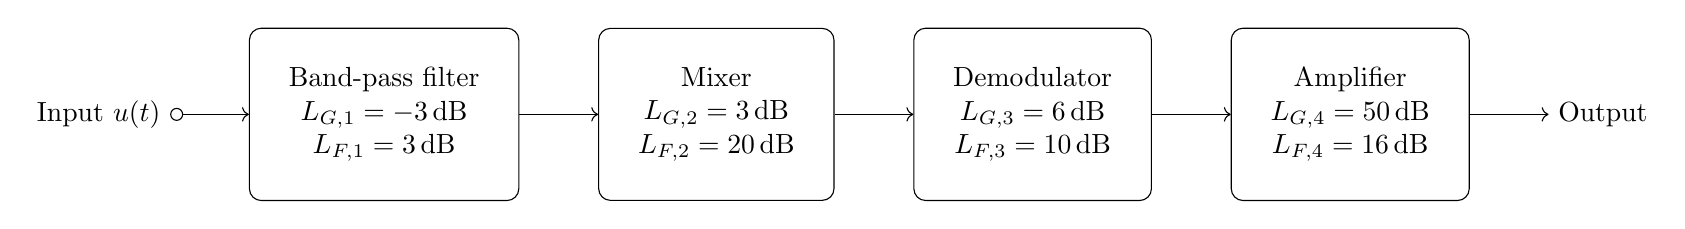
\begin{tikzpicture}
				\node[draw, block] (BPF){Band-pass filter\\ $L_{G,1} = \SI{-3}{dB}$\\ $L_{F,1} = \SI{3}{dB}$};
				\node[draw, block, right=of BPF] (Mix){Mixer\\ $L_{G,2} = \SI{3}{dB}$\\ $L_{F,2} = \SI{20}{dB}$};
				\node[draw, block, right=of Mix] (Demod){Demodulator\\ $L_{G,3} = \SI{6}{dB}$\\ $L_{F,3} = \SI{10}{dB}$};
				\node[draw, block, right=of Demod] (Amp){Amplifier\\ $L_{G,4} = \SI{50}{dB}$\\ $L_{F,4} = \SI{16}{dB}$};
				
				\draw[o->] ([xshift=-1cm]BPF.west) node[left,align=right]{Input $u(t)$} -- (BPF.west);
				\draw[->] (BPF.east) -- (Mix.west);
				\draw[->] (Mix.east) -- (Demod.west);
				\draw[->] (Demod.east) -- (Amp.west);
				\draw[->] (Amp.east) -- ([xshift=1cm]Amp.east) node[right,align=left]{Output};
			\end{tikzpicture}
		\end{adjustbox}
	\end{figure}
	\begin{itemize}
		\item The band-pass filter has an input impedance of $\SI{50}{\ohm}$.
		\item The band-pass filter has a bandwidth of $\SI{2}{MHz}$.
		\item All system components are at room temperature: \SI{25}{\degreeCelsius}.
	\end{itemize}
	The input signal is:
	\begin{equation*}
		u(t) = \SI{70.71}{\micro\volt} \cdot \cos\left(\omega_0 t\right)
	\end{equation*}
	
	Give all results in the logarithmic scale!
	\begin{tasks}
		\task
		What is the signal power, the thermal noise power and the SNR at the input?
		
		\task
		What is the overall noise figure and overall gain of the chain? What is the signal power, the thermal noise power and the SNR at the output of the chain?
		
		\task
		Now a low noise amplifier is placed in front of the mixer. The gain of the last amplifier is reduced, so that the overall gain does not change.
		\begin{figure}[H]
			\centering
			\begin{adjustbox}{scale=0.5}
				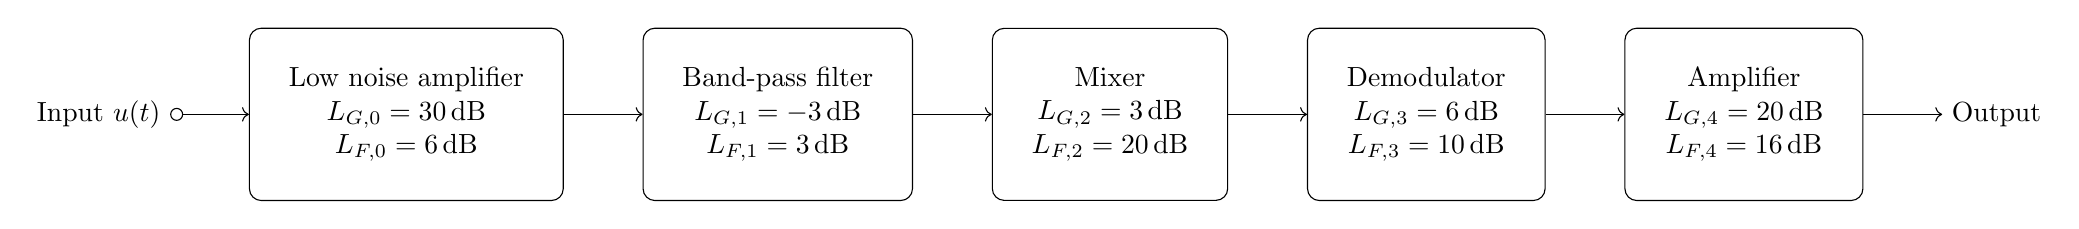
\begin{tikzpicture}
					\node[draw, block] (Amp){Low noise amplifier\\ $L_{G,0} = \SI{30}{dB}$\\ $L_{F,0} = \SI{6}{dB}$};
					\node[draw, block, right=of Amp] (BPF){Band-pass filter\\ $L_{G,1} = \SI{-3}{dB}$\\ $L_{F,1} = \SI{3}{dB}$};
					\node[draw, block, right=of BPF] (Mix){Mixer\\ $L_{G,2} = \SI{3}{dB}$\\ $L_{F,2} = \SI{20}{dB}$};
					\node[draw, block, right=of Mix] (Demod){Demodulator\\ $L_{G,3} = \SI{6}{dB}$\\ $L_{F,3} = \SI{10}{dB}$};
					\node[draw, block, right=of Demod] (Amp2){Amplifier\\ $L_{G,4} = \SI{20}{dB}$\\ $L_{F,4} = \SI{16}{dB}$};
					
					\draw[o->] ([xshift=-1cm]Amp.west) node[left,align=right]{Input $u(t)$} -- (Amp.west);
					\draw[->] (Amp.east) -- (BPF.west);
					\draw[->] (BPF.east) -- (Mix.west);
					\draw[->] (Mix.east) -- (Demod.west);
					\draw[->] (Demod.east) -- (Amp2.west);
					\draw[->] (Amp2.east) -- ([xshift=1cm]Amp2.east) node[right,align=left]{Output};
				\end{tikzpicture}
			\end{adjustbox}
		\end{figure}
		For this new constellation: What is the overall noise figure and overall gain of the chain? What is the signal power, the thermal noise power and the SNR at the output of the chain?
	\end{tasks}
\end{question}

\begin{solution}
	\begin{tasks}
		\task
		\begin{itemize}
			\item The RMS value of the signals is: $\frac{\SI{70.71}{\micro\volt}}{\sqrt{2}} = \SI{50}{\micro\volt}$
			\item At $\SI{50}{\ohm}$, this yields a power of: $P = \frac{U^2}{R} = \SI{50}{pW} \equiv L_{P,S} = \SI{-73}{dBm}$
			\item The noise floor at room temperature is: $k_B T \equiv \SI{-174}{dBm/Hz}$
			\item The filter's bandwidth is: $\SI{63}{dBHz}$
			\item The noise power is: $k_B T \Delta f \equiv L_{P,N} = \SI{-174}{dBm/Hz} + \SI{63}{dBHz} = \SI{-111}{dBm}$
			\item The SNR is: $L_{\mathrm{SNR}} = L_{P,S} - L_{P,N} = \SI{-73}{dBm} - (\SI{-111}{dBm}) = \SI{38}{dBm}$
		\end{itemize}
	
		\task
		Convert to linear scale:
		\begin{itemize}
			\item $G_1 = 0.5$
			\item $F_1 = 2$
			\item $G_2 = 2$
			\item $F_2 = 100$
			\item $G_3 = 4$
			\item $F_3 = 10$
			\item $G_4 = 100000$
			\item $F_4 = 40$
		\end{itemize}
	
		Using the Friis formula:
		\begin{equation*}
			\begin{split}
				F_{\text{total}} &= F_1 + \frac{F_2 - 1}{G_1} + \frac{F_3 - 1}{G_1 G_2} + \frac{F_4 - 1}{G_1 G_2 G_3} \\
				 &= 218 \\
				L_{F,\text{total}} &= \SI{23.4}{dB}
			\end{split}
		\end{equation*}
		Overall gain:
		\begin{equation*}
			L_{G,\text{total}} = \SI{-3}{dB} + \SI{3}{dB} + \SI{6}{dB} + \SI{50}{dB} = \SI{56}{dB}
		\end{equation*}
		\begin{itemize}
			\item Output signal power: $\SI{-73}{dBm} + L_{G,\text{total}} = \SI{-17}{dBm}$
			\item Output noise power: $\SI{-111}{dBm} + L_{G,\text{total}} + L_{F,\text{total}} = \SI{-31.6}{dBm}$
			\item Output SNR: $\SI{38}{dBm} - L_{F,\text{total}} = \SI{14.6}{dB}$
		\end{itemize}
	
		\task
		Convert to linear scale:
		\begin{itemize}
			\item $G_0 = 1000$
			\item $F_0 = 4$
			\item $G_1 = 0.5$
			\item $F_1 = 2$
			\item $G_2 = 2$
			\item $F_2 = 100$
			\item $G_3 = 4$
			\item $F_3 = 10$
			\item $G_4 = 10$
			\item $F_4 = 40$
		\end{itemize}
	
		Using the Friis formula:
		\begin{equation*}
			\begin{split}
				F_{\text{total}} &= F_0 + \frac{F_1 - 1}{G_0} + \frac{F_2 - 1}{G_0 G_1} + \frac{F_3 - 1}{G_0 G_1 G_2} + \frac{F_4 - 1}{G_0 G_1 G_2 G_3} \\
				 &= 4.22 \\
				L_{F,\text{total}} &= \SI{6.3}{dB}
			\end{split}
		\end{equation*}
		Overall gain:
		\begin{equation*}
			L_{G,\text{total}} = \SI{50}{dB} + \SI{-3}{dB} + \SI{3}{dB} + \SI{6}{dB} = \SI{56}{dB}
		\end{equation*}
		\begin{itemize}
			\item Output signal power: $\SI{-73}{dBm} + L_{G,\text{total}} = \SI{-17}{dBm}$
			\item Output noise power: $\SI{-111}{dBm} + L_{G,\text{total}} + L_{F,\text{total}} = \SI{-48.7}{dBm}$
			\item Output SNR: $\SI{38}{dBm} - L_{F,\text{total}} = \SI{31.7}{dB}$
		\end{itemize}
	
		\textbf{Conclusion:}
		\begin{itemize}
			\item Placing the low noise amplifier in front of the chain, gives a much better ($\SI{16.1}{dB}$) SNR. The gain is equal.
			\item The overall noise figure is dominated by the first component in the chain.
			\item In this constellation, first component is a low noise amplifier with high gain and low noise figure.
			\item The high gain scales down the noise contribution of the components following in the chain.
			\item Therefore, it is always feasible to place a low noise amplifier (high gain, low noise) to the front of the chain.
		\end{itemize}
	\end{tasks}
\end{solution}

\begin{question}[subtitle={Python Programming: Cross-correlation}]
Solve all tasks in Python!

Three signal samples are provided along with this exercise. Which one correlates most with the Gauss pulse given in the Python template file?

Make plots and decide from them!
\end{question}

\begin{solution}
\end{solution}



%%%%%%%%%%%%%%%%%%%%%%%%%%%%%%%%%%%%%%%%%%%%%%%%%%%%%%%%%%%%%%%%%%%%%%%%%%%%%%%
%\begin{question}[subtitle={Decibel}]
%	\begin{tasks}
%	\end{tasks}
%\end{question}
%
%\begin{solution}
%	\begin{tasks}
%	\end{tasks}
%\end{solution}

\clearpage

\chapter{Sampling and Time-Discrete Signals and Systems}

\begin{refsection}

\section{Time-Discrete Signals}

\subsection{Ideal Sampling}

\begin{figure}[H]
	\centering
	\begin{tikzpicture}
		\begin{axis}[
			height={0.25\textheight},
			width=0.6\linewidth,
			scale only axis,
			xlabel={$t$},
			ylabel={$x$},
			%grid style={line width=.6pt, color=lightgray},
			%grid=both,
			grid=none,
			legend pos=north west,
			axis y line=middle,
			axis x line=middle,
			every axis x label/.style={
				at={(ticklabel* cs:1.05)},
				anchor=north,
			},
			every axis y label/.style={
				at={(ticklabel* cs:1.05)},
				anchor=east,
			},
			%xmin=0,
			%xmax=7,
			%ymin=0,
			%ymax=3,
			%xtick={0, 1, ..., 6},
			%ytick={0, 0.5, ..., 2.5},
			xmin=0,
			xmax=6.5,
			xtick={0, 1, ..., 6},
			xticklabels={$0$, $T_S$, $2 T_S$, $3 T_S$, $4 T_S$, $5 T_S$, $6 T_S$},
		]
			\addplot[smooth, blue, dashed] coordinates {(0, 1.1) (1, 1.8) (2, 2.1) (3, 1.0) (4, 0.8) (5, 1.7) (6, 2.4)};
			\addlegendentry{$\underline{x}{t}$};
			\addplot[red, thick] coordinates {(0, 0) (0, 1.1)};
			\addplot[red, thick] coordinates {(1, 0) (1, 1.8)};
			\addplot[red, thick] coordinates {(2, 0) (2, 2.1)};
			\addplot[red, thick] coordinates {(3, 0) (3, 1.0)};
			\addplot[red, thick] coordinates {(4, 0) (4, 0.8)};
			\addplot[red, thick] coordinates {(5, 0) (5, 1.7)};
			\addplot[red, thick] coordinates {(6, 0) (6, 2.4)};
			\addplot[only marks, red, thick, mark=o] coordinates {(0, 1.1) (1, 1.8) (2, 2.1) (3, 1.0) (4, 0.8) (5, 1.7) (6, 2.4)};
			\addlegendentry{$\underline{x}_S{t}$};
		\end{axis}
	\end{tikzpicture}
	\caption{Sampling of a time-continuous signal}
	\label{fig:ch04:sampling_of_signal}
\end{figure}

Sampling:
\begin{itemize}
	\item Sampling is converting a time-continuous signal $\underline{x}(t)$ to a time-discrete signal $\underline{x}[n]$.
	\item Samples are periodically taken out of the original signal.
\end{itemize}

Nomenclature:
\begin{itemize}
	\item The original time-continuous signal is $\underline{x}(t)$. The continuous time variable $t \in \mathbb{R}$ is a continuous real number.
	\item The sampled signal is $\underline{x}[n]$. The discrete time variable $n \in \mathbb{Z}$ is a (discrete) integer number.
	\item Round parenthesis is used for time-continuous signals. Square parenthesis is used for time-discrete signals.
\end{itemize}

Sampling parameters:
\begin{itemize}
	\item The time instances, at which the samples are taken out, are equidistant.
	\item The period between the samples is the \index{sampling period} \textbf{sampling period} $T_S$.
	\item The inverse of the sampling period is the \index{sampling rate} \textbf{sampling rate} $f_S$.
	\begin{equation}
		f_S = \frac{1}{T_S}
	\end{equation}
	\item The \index{sampling angular frequency} \textbf{sampling angular frequency} $\omega_S$.
	\begin{equation}
		\omega_S = \frac{2 \pi}{T_S}
	\end{equation}
\end{itemize}

Ideal sampling:
\begin{itemize}
	\item The samples are ideally equidistant. The sampling period $T_S$ is constant and is \underline{not} subject to fluctuations.
	\item The sample has the value of the original signal $\underline{x}(t)$ at \underline{exactly} the time instance where has been taken.
\end{itemize}
Some corollaries can be deducted from these two points:
\begin{itemize}
	\item The sampled signal $\underline{x}_S(n T_S)$ at the discrete time $n$ is the value of the original signal at time $t = n T_S$.
	\begin{equation}
		\underline{x}[n] = \underline{x}\left(n T_S\right)
	\end{equation}
	\item The sampled signal $\underline{x}_S(t)$ consists of a chain of equidistant, indefinitely narrow pulses.
	\begin{itemize}
		\item The pulses are equidistant with $T_S$.
		\item The pulses have the value of $\underline{x}\left(n T_S\right)$ as their amplitudes.
		\item The value of the sampled signal is zero in between the pulses.
		\begin{equation}
			\underline{x}_S(t) = \begin{cases}
				\underline{x}\left(n T_S\right) & \quad \forall \; t = n T_S, n \in \mathbb{Z}, \\
				0 & \quad \forall \; n T_S < t < \left(n+1\right) T_S, n \in \mathbb{Z}.
			\end{cases}
		\end{equation}
	\end{itemize}
\end{itemize}

\subsubsection{Dirac comb}

We know already indefinitely narrow pulses. They are Dirac delta functions $\delta\left(t - n T_S\right)$.

Taking out \underline{exactly one} sample out of $\underline{x}(t)$ is a multiplication of $\underline{x}(t)$ with $\delta\left(t - n T_S\right)$.
\begin{equation}
	\underline{x}_{S,n}(t) = \underline{x}(t) \delta\left(t - n T_S\right)
	\label{eq:ch4:one_sample_1}
\end{equation}
The Dirac delta function is zero expect at $t = n T_S$. So, \eqref{eq:ch4:one_sample_1} can be further reduced.
\begin{equation}
	\underline{x}_{S,n}(t) = \underline{x}(n T_S) \delta\left(t - n T_S\right)
	\label{eq:ch4:one_sample_2}
\end{equation}

\begin{figure}[H]
	\centering
	\begin{tikzpicture}
		\begin{axis}[
			height={0.25\textheight},
			width=0.6\linewidth,
			scale only axis,
			xlabel={$t$},
			ylabel={$x$},
			%grid style={line width=.6pt, color=lightgray},
			%grid=both,
			grid=none,
			legend pos=north west,
			axis y line=middle,
			axis x line=middle,
			every axis x label/.style={
				at={(ticklabel* cs:1.05)},
				anchor=north,
			},
			every axis y label/.style={
				at={(ticklabel* cs:1.05)},
				anchor=east,
			},
			%xmin=0,
			%xmax=7,
			%ymin=0,
			%ymax=3,
			%xtick={0, 1, ..., 6},
			%ytick={0, 0.5, ..., 2.5},
			xmin=0,
			xmax=6.5,
			xtick={0, 1, ..., 6},
			xticklabels={$0$, $T_S$, $2 T_S$, $3 T_S$, $4 T_S$, $5 T_S$, $6 T_S$},
		]
			\addplot[smooth, blue, dashed] coordinates {(0, 1.1) (1, 1.8) (2, 2.1) (3, 1.0) (4, 0.8) (5, 1.7) (6, 2.4)};
			\addlegendentry{$\underline{x}{t}$};
			\addplot[red, thick] coordinates {(2, 0) (2, 2.1)};
			\addplot[only marks, red, thick, mark=o] coordinates {(2, 2.1)};
			\addlegendentry{$\underline{x}_{S,n}{t}$};
		\end{axis}
	\end{tikzpicture}
	\caption[Taking out exactly one sample out of $\underline{x}(t)$]{Taking out exactly one sample out of $\underline{x}(t)$ -- in this example $n = 2$.}
\end{figure}

To obtain the sampled signal, the sampling process $\underline{x}_{S,n}(t)$ \eqref{eq:ch4:one_sample_1} needs to be repeated for each $n \in \mathbb{Z}$. All individual sample processes $\underline{x}_{S,n}(t)$ are then superimposed to form the complete sampled signal $\underline{x}_S(t)$.
\begin{equation}
	\begin{split}
		\underline{x}_S(t) &= \sum\limits_{n = -\infty}^{\infty} \underline{x}_{S,n}(t) \\
		 &= \sum\limits_{n = -\infty}^{\infty} \underline{x}\left(t\right) \delta\left(t - n T_S\right) \\
		 &= \underline{x}\left(t\right) \cdot \underbrace{\sum\limits_{n = -\infty}^{\infty} \delta\left(t - n T_S\right)}_{= \Sha_{T_S}(t)}
	\end{split}
\end{equation}

The sum of Dirac delta functions
\begin{itemize}
	\item forms a series of equidistant pulses repeating at a period of $T_S$,
	\item is called \index{Dirac comb} \textbf{Dirac comb} $\Sha_{T_S}(t)$ or \index{impulse train} \textbf{impulse train}.
\end{itemize}

\begin{definition}{Dirac comb}
	The \index{Dirac comb} \textbf{Dirac comb} $\Sha_{T}(t)$ or \index{impulse train} \textbf{impulse train} is:
	\begin{equation}
		\Sha_{T}(t) = \sum\limits_{n = -\infty}^{\infty} \delta\left(t - n T\right)
		\label{eq:ch04:dirac_comb}
	\end{equation}
	$T$ is the period of the equidistant Dirac pulses.
	
	It is a periodic signal and can be decomposed using the Fourier analysis:
	\begin{equation}
		\Sha_{T}(t) = \frac{1}{T} \sum\limits_{n = -\infty}^{\infty} e^{j n \frac{2 \pi}{T} t}
		\label{eq:ch04:dirac_comb_fourier_series}
	\end{equation}
	
	\begin{figure}[H]
		\centering
		\begin{tikzpicture}
			\begin{axis}[
				height={0.15\textheight},
				width=0.9\linewidth,
				scale only axis,
				xlabel={$t$},
				ylabel={$\Sha_{T_S}(t)$},
				%grid style={line width=.6pt, color=lightgray},
				%grid=both,
				grid=none,
				legend pos=north east,
				axis y line=middle,
				axis x line=middle,
				every axis x label/.style={
					at={(ticklabel* cs:1.05)},
					anchor=north,
				},
				every axis y label/.style={
					at={(ticklabel* cs:1.05)},
					anchor=east,
				},
				xmin=-5.5,
				xmax=5.5,
				ymin=0,
				ymax=1.2,
				xtick={-5, -4, ..., 5},
				xticklabels={$-5 T_S$, $-4 T_S$, $-3 T_S$, $-2 T_S$, $- T_S$, $0$, $T_S$, $2 T_S$, $3 T_S$, $4 T_S$, $5 T_S$},
				ytick={0},
			]
				\pgfplotsinvokeforeach{-5, -4, ..., 5}{
					\draw[-latex, blue, very thick] (axis cs:#1,0) -- (axis cs:#1,1);
					%\addplot[blue, very thick] coordinates {(#1, 0) (#1, 1)};
					%\addplot[only marks, blue, thick, mark=triangle] coordinates {(#1, 1)};
				}
			\end{axis}
		\end{tikzpicture}
		\caption{Dirac comb}
	\end{figure}
\end{definition}

\subsubsection{Ideal Sampler}

A \index{sampler} \textbf{sampler} is a system which
\begin{itemize}
	\item applies the Dirac comb $\Sha_{T_S}(t)$
	\item to a time-continuous signal $\underline{x}(t)$ (multiplication) and
	\item outputs a series of equidistant pulses $\underline{x}_S(t)$.
\end{itemize}

\begin{definition}{Ideally sampled signal}
	An ideally \index{sampled signal} sampled signal is:
	\begin{equation}
		\begin{split}
			\underline{x}_S(t) &= \underline{x}(t) \cdot \Sha_{T_S}(t) \\
			 &= \sum\limits_{n = -\infty}^{\infty} \underline{x}\left(t\right) \delta\left(t - n T_S\right) \\
			 &= \sum\limits_{n = -\infty}^{\infty} \underline{x}\left(n T_S\right) \delta\left(t - n T_S\right)
		\end{split}
		\label{eq:ch04:ideal_sampling}
	\end{equation}
\end{definition}

The sampled signal $\underline{x}_S(t)$ is a chain of pulses (red signal in Figure \ref{fig:ch04:sampling_of_signal}). The chain of pulses can then be reinterpreted as a time-discrete signal $\underline{x}[n]$. The value of $\underline{x}[n]$ is:
\begin{equation}
	\underline{x}[n] = \underline{x}_S\left(n T_S\right) = \underline{x}\left(n T_S\right) \qquad \forall \; n \in \mathbb{Z}
	\label{eq:ch04:sample_value}
\end{equation}

\begin{figure}[H]
	\centering
	\begin{adjustbox}{scale=0.8}
		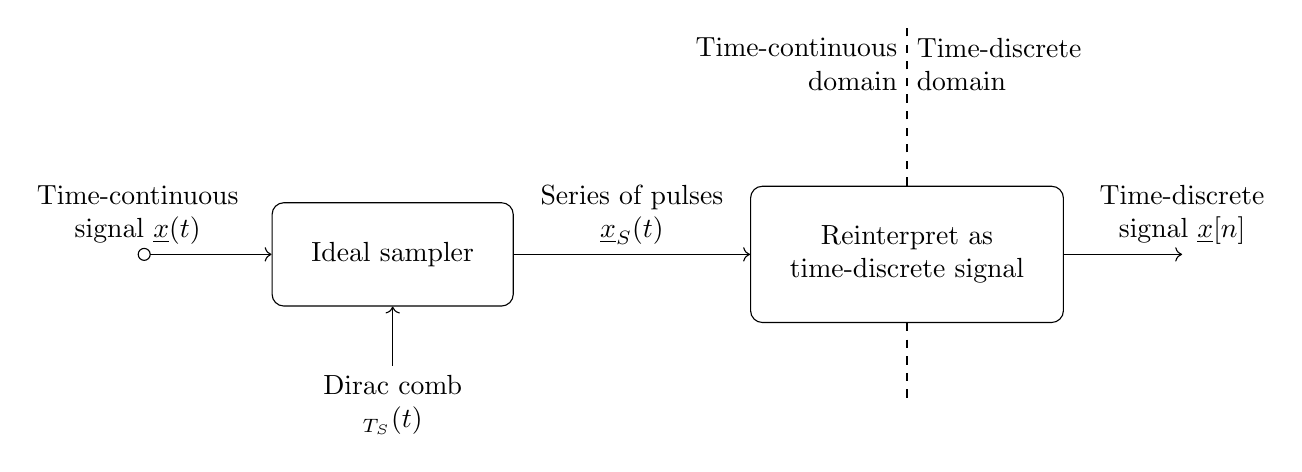
\begin{tikzpicture}
			\node[draw, block] (Sampler) {Ideal sampler};
			\node[draw, block, right=3cm of Sampler] (ReInterp) {Reinterpret as\\ time-discrete signal};
			
			\draw[<-o] (Sampler.west) -- ++(-1.7cm, 0) node[above, align=center]{Time-continuous\\ signal $\underline{x}(t)$};
			\draw[->] (Sampler.east) -- (ReInterp.west) node[midway, above, align=center]{Series of pulses\\ $\underline{x}_S(t)$};
			\draw[<-] (Sampler.south) -- ++(0, -0.75cm) node[below, align=center]{Dirac comb\\ $\Sha_{T_S}(t)$};
			\draw[->] (ReInterp.east) -- ++(1.5cm, 0) node[above, align=center]{Time-discrete\\ signal $\underline{x}[n]$};
			
			\draw[dashed] (ReInterp.north) -- ++(0, 2cm) node[below left, align=right]{Time-continuous\\ domain} node[below right, align=left]{Time-discrete\\ domain};
			\draw[dashed] (ReInterp.south) -- ++(0, -1cm);
		\end{tikzpicture}
	\end{adjustbox}
	\caption{An abstract view on sampling}
\end{figure}

\subsubsection{Irreversibility of Sampling}

\begin{fact}
	The act of sampling is irreversible.
\end{fact}
	
There is a way to obtain the sampled signal:
\begin{equation*}
	\underline{x}_S(t) = \mathrm{Sampling} \left(\underline{x}(t)\right)
\end{equation*}
But there is generally no way back to reconstruct the original signal. $\mathrm{Sampling}^{-1} \left(\underline{x}_S(t)\right)$ does not exist.
\begin{equation*}
	\underline{x}(t) \neq \underbrace{\mathrm{Sampling}^{-1}}_{\text{Does not exist}} \left(\underline{x}_S(t)\right)
\end{equation*}

Sampling is always lossy in general.

\subsection{Sampling Theorem, Aliasing and Reconstruction}

\subsubsection{Frequency Domain Representation}

\begin{excursus}{Fourier transform of the Dirac comb}
	The Fourier transform of the Dirac comb is again a Dirac comb:
	\begin{equation}
		\begin{split}
			\Sha_{T}(t) \TransformHoriz \mathcal{F}\left\{\Sha_{T}(t)\right\} &= \frac{2 \pi}{T} \Sha_{\frac{2 \pi}{T}}(\omega) \\
			 &= \frac{2 \pi}{T} \sum\limits_{k = -\infty}^{\infty} \delta\left(\omega - k \frac{2 \pi}{T}\right) \\
			 &= \sum\limits_{k = -\infty}^{\infty} e^{- j \omega k T}
		\end{split}
		\label{eq:ch04:dirac_comb_fourier_tranform}
	\end{equation}
\end{excursus}

\eqref{eq:ch04:ideal_sampling} pointed out, that the sampled signal $\underline{x}_S(t)$ is the multiplication of the original time-domain signal $\underline{x}(t)$ and the Dirac comb $\Sha_{T_S}(t)$ with a periodicity of the sampling period $T_S$.
\begin{equation}
	\begin{split}
		\underline{x}_S(t) &= \underline{x}(t) \cdot \Sha_{T_S}(t) \\
		 &= \underline{x}(t) \cdot \frac{1}{T_S} \sum\limits_{n = -\infty}^{\infty} e^{j n \frac{2 \pi}{T_S} t} \\
		 &= \frac{1}{T_S} \sum\limits_{n = -\infty}^{\infty} \underbrace{\underline{x}(t) e^{j n \frac{2 \pi}{T_S} t}}_{\text{Frequency shift by } n \frac{2 \pi}{T_S}} \\
	\end{split}
\end{equation}

The ideally sampled signal $\underline{x}_S(t)$ can be expressed as a sum of \emph{frequency shifts} of the original signal $\underline{x}(t)$. Its Fourier transform is:
\begin{equation}
	\begin{split}
		\underline{X}_S\left(j \omega\right) &= \mathcal{F}\left\{\frac{1}{T_S} \sum\limits_{k = -\infty}^{\infty} \underline{x}(t) e^{j k \frac{2 \pi}{T_S} t}\right\} \\
		 & \qquad \text{Using the linearity of the Fourier transform:} \\
		 &= \frac{1}{T_S} \sum\limits_{k = -\infty}^{\infty} \mathcal{F}\left\{\underline{x}(t) e^{j k \frac{2 \pi}{T_S} t}\right\} \\
		 & \qquad \text{Using the frequency shift theorem of the Fourier transform:} \\
		 &= \frac{1}{T_S} \sum\limits_{k = -\infty}^{\infty} \underline{X}\left(j \left(\omega - k \frac{2 \pi}{T_S} \right)\right)
	\end{split}
\end{equation}

\begin{proof}{}
	An alternative way is using the Fourier transform of this multiplication in the time-domain is a convolution in the frequency domain:
	\begin{equation}
		\begin{split}
			\underline{X}_S\left(j \omega\right) &= \mathcal{F}\left\{\underline{x}(t) \cdot \Sha_{T_S}(t)\right\} \\
			 &= \frac{1}{2 \pi} \underline{X}\left(j \omega\right) * \left(\frac{2 \pi}{T_S} \Sha_{\frac{2 \pi}{T_S}}(\omega)\right) \\
			 &= \frac{1}{T_S} \int\limits_{-\infty}^{\infty} \underline{X}\left(j \left(\omega - \zeta\right)\right) \Sha_{\frac{2 \pi}{T_S}}\left(\zeta\right) \, \mathrm{d} \zeta \\
			 &= \frac{1}{T_S} \int\limits_{-\infty}^{\infty} \underline{X}\left(j \left(\omega - \zeta\right)\right) \sum\limits_{k = -\infty}^{\infty} \delta\left(\zeta - k \frac{2 \pi}{T_S}\right) \, \mathrm{d} \zeta \\
			 &= \frac{1}{T_S} \sum\limits_{k = -\infty}^{\infty} \int\limits_{-\infty}^{\infty} \underline{X}\left(j \left(\omega - \zeta\right)\right) \delta\left(\zeta - k \frac{2 \pi}{T_S}\right) \, \mathrm{d} \zeta \\
			 & \qquad \text{Using the Dirac measure:} \\
			 &= \frac{1}{T_S} \sum\limits_{k = -\infty}^{\infty} \underline{X}\left(j \left(\omega - k \frac{2 \pi}{T_S}\right)\right) \\
		\end{split}
	\end{equation}
\end{proof}

\textbf{Conclusion:} The spectrum of the sampled signal $\underline{X}_S\left(j \omega\right)$
\begin{itemize}
	\item consists of superimposed, frequency-shifted copies of the spectra of the original signal $\underline{X}\left(j\omega\right)$ and
	\item the periodicity of the superimposed, frequency-shifted copies is the sampling angular frequency $\omega_S = \frac{2 \pi}{T_S}$ or sampling frequency $f_S$, respectively,
	\item each frequency-shifted copy starts at $k \omega_S - \frac{\omega_S}{2}$ and ends at $k \omega_S + \frac{\omega_S}{2}$.
\end{itemize}

\begin{figure}[H]
	\subfloat[Original signal $\underline{X}\left(j\omega\right)$] {
		\centering
		\begin{tikzpicture}
				\begin{axis}[
				height={0.15\textheight},
				width=0.9\linewidth,
				scale only axis,
				xlabel={$\omega$},
				ylabel={$|\underline{X}\left(j\omega\right)|$},
				%grid style={line width=.6pt, color=lightgray},
				%grid=both,
				grid=none,
				legend pos=north east,
				axis y line=middle,
				axis x line=middle,
				every axis x label/.style={
					at={(ticklabel* cs:1.05)},
					anchor=north,
				},
				every axis y label/.style={
					at={(ticklabel* cs:1.05)},
					anchor=east,
				},
				xmin=-3.5,
				xmax=3.5,
				ymin=0,
				ymax=1.2,
				xtick={-1, -0.5, 0, 0.5, 1},
				xticklabels={$- \omega_S$, $- \frac{\omega_S}{2}$, $0$, $\frac{\omega_S}{2}$, $\omega_S$},
				ytick={0},
			]
				\draw[green, thick] (axis cs:-0.4,0) -- (axis cs:0,0.7);
				\draw[red, thick] (axis cs:0,0.7) -- (axis cs:0.4,0);
			\end{axis}
		\end{tikzpicture}
	}

	\subfloat[Spectrum of the Dirac comb $\frac{2 \pi}{T} \Sha_{\frac{2 \pi}{T}}(\omega)$] {
		\centering
		\begin{tikzpicture}
			\begin{axis}[
				height={0.15\textheight},
				width=0.9\linewidth,
				scale only axis,
				xlabel={$t$},
				ylabel={$|\frac{2 \pi}{T} \Sha_{\frac{2 \pi}{T}}(\omega)|$},
				%grid style={line width=.6pt, color=lightgray},
				%grid=both,
				grid=none,
				legend pos=north east,
				axis y line=middle,
				axis x line=middle,
				every axis x label/.style={
					at={(ticklabel* cs:1.05)},
					anchor=north,
				},
				every axis y label/.style={
					at={(ticklabel* cs:1.05)},
					anchor=east,
				},
				xmin=-3.5,
				xmax=3.5,
				ymin=0,
				ymax=1.2,
				xtick={-3, -2, ..., 3},
				xticklabels={$-3 \omega_S$, $-2 \omega_S$, $- \omega_S$, $0$, $\omega_S$, $2 \omega_S$, $3 \omega_S$},
				ytick={0},
			]
				\pgfplotsinvokeforeach{-3, -2, ..., 3}{
					\draw[-latex, blue, very thick] (axis cs:#1,0) -- (axis cs:#1,1);
				}
			\end{axis}
		\end{tikzpicture}
	}

	\subfloat[Sampled signal $\underline{X}_S\left(j\omega\right)$] {
	\centering
	\begin{tikzpicture}
		\begin{axis}[
			height={0.15\textheight},
			width=0.9\linewidth,
			scale only axis,
			xlabel={$\omega$},
			ylabel={$|\underline{X}_S\left(j\omega\right)|$},
			%grid style={line width=.6pt, color=lightgray},
			%grid=both,
			grid=none,
			legend pos=north east,
			axis y line=middle,
			axis x line=middle,
			every axis x label/.style={
				at={(ticklabel* cs:1.05)},
				anchor=north,
			},
			every axis y label/.style={
				at={(ticklabel* cs:1.05)},
				anchor=east,
			},
			xmin=-3.5,
			xmax=3.5,
			ymin=0,
			ymax=1.2,
			xtick={-3, -2, -1, -0.5, 0, 0.5, 1, 2, 3},
			xticklabels={$-3 \omega_S$, $-2 \omega_S$, $- \omega_S$, $- \frac{\omega_S}{2}$, $0$, $\frac{\omega_S}{2}$, $\omega_S$, $2 \omega_S$, $3 \omega_S$},
			ytick={0},
		]
			\pgfplotsinvokeforeach{-3, -2, ..., 3}{
				\draw[-latex, blue, dashed, very thick] (axis cs:#1,0) -- (axis cs:#1,1);
				\draw[green, thick] (axis cs:{#1-0.4},0) -- (axis cs:#1,0.7);
				\draw[red, thick] (axis cs:#1,0.7) -- (axis cs:{#1+0.4},0);
			}
		\end{axis}
	\end{tikzpicture}
	}

	\caption{Spectrum of the sampled signal}
\end{figure}

\begin{attention}
	The spectrum of the original signal $\underline{X}\left(j\omega\right)$ has both negative and positive frequencies. Remember that the symmetry rules apply \underline{only} for real-valued time-domain signals.
\end{attention}

\subsubsection{Aliasing}

The original signal in the previous example was limited to $- \frac{\omega_S}{2} \leq \omega \leq \frac{\omega_S}{2}$. The spectrum sampled signal consists of the frequency-shifted copies of the original signal's spectrum. Although they are superimposed, they do not overlap.

A problem arises when the original signal is \underline{not} limited to $- \frac{\omega_S}{2} \leq \omega \leq \frac{\omega_S}{2}$. The original signal's spectrum will overlap.

\begin{figure}[H]
	\subfloat[Original signal $\underline{X}\left(j\omega\right)$ violating the band-limitation $- \frac{\omega_S}{2} \leq \omega \leq \frac{\omega_S}{2}$. The original signal's spectrum will overlap.
	] {
		\centering
		\begin{tikzpicture}
			\begin{axis}[
				height={0.15\textheight},
				width=0.9\linewidth,
				scale only axis,
				xlabel={$\omega$},
				ylabel={$|\underline{X}\left(j\omega\right)|$},
				%grid style={line width=.6pt, color=lightgray},
				%grid=both,
				grid=none,
				legend pos=north east,
				axis y line=middle,
				axis x line=middle,
				every axis x label/.style={
					at={(ticklabel* cs:1.05)},
					anchor=north,
				},
				every axis y label/.style={
					at={(ticklabel* cs:1.05)},
					anchor=east,
				},
				xmin=-3.5,
				xmax=3.5,
				ymin=0,
				ymax=1.2,
				xtick={-3, -2, -1, -0.5, 0, 0.5, 1, 2, 3},
				xticklabels={$-3 \omega_S$, $-2 \omega_S$, $- \omega_S$, $- \frac{\omega_S}{2}$, $0$, $\frac{\omega_S}{2}$, $\omega_S$, $2 \omega_S$, $3 \omega_S$},
				ytick={0},
			]
				\draw[green, thick] (axis cs:-0.7,0) -- (axis cs:0,0.7);
				\draw[red, thick] (axis cs:0,0.7) -- (axis cs:0.8,0);
				\draw[olive, thick] (axis cs:2.1,0) -- (axis cs:2.1,0.5) -- (axis cs:2.3,0.5) -- (axis cs:2.3,0);
			\end{axis}
		\end{tikzpicture}
	}
	
	\subfloat[Spectrum of the Dirac comb $\frac{2 \pi}{T} \Sha_{\frac{2 \pi}{T}}(\omega)$] {
		\centering
		\begin{tikzpicture}
		\begin{axis}[
		height={0.15\textheight},
		width=0.9\linewidth,
		scale only axis,
		xlabel={$t$},
		ylabel={$|\frac{2 \pi}{T} \Sha_{\frac{2 \pi}{T}}(\omega)|$},
		%grid style={line width=.6pt, color=lightgray},
		%grid=both,
		grid=none,
		legend pos=north east,
		axis y line=middle,
		axis x line=middle,
		every axis x label/.style={
			at={(ticklabel* cs:1.05)},
			anchor=north,
		},
		every axis y label/.style={
			at={(ticklabel* cs:1.05)},
			anchor=east,
		},
		xmin=-3.5,
		xmax=3.5,
		ymin=0,
		ymax=1.2,
		xtick={-3, -2, ..., 3},
		xticklabels={$-3 \omega_S$, $-2 \omega_S$, $- \omega_S$, $0$, $\omega_S$, $2 \omega_S$, $3 \omega_S$},
		ytick={0},
		]
		\pgfplotsinvokeforeach{-3, -2, ..., 3}{
			\draw[-latex, blue, very thick] (axis cs:#1,0) -- (axis cs:#1,1);
		}
		\end{axis}
		\end{tikzpicture}
	}
	
	\subfloat[Sampled signal $\underline{X}_S\left(j\omega\right)$ showing aliasing] {
		\centering
		\begin{tikzpicture}
		\begin{axis}[
		height={0.15\textheight},
		width=0.9\linewidth,
		scale only axis,
		xlabel={$\omega$},
		ylabel={$|\underline{X}_S\left(j\omega\right)|$},
		%grid style={line width=.6pt, color=lightgray},
		%grid=both,
		grid=none,
		legend pos=north east,
		axis y line=middle,
		axis x line=middle,
		every axis x label/.style={
			at={(ticklabel* cs:1.05)},
			anchor=north,
		},
		every axis y label/.style={
			at={(ticklabel* cs:1.05)},
			anchor=east,
		},
		xmin=-3.5,
		xmax=3.5,
		ymin=0,
		ymax=1.2,
		xtick={-3, -2, -1, -0.5, 0, 0.5, 1, 2, 3},
		xticklabels={$-3 \omega_S$, $-2 \omega_S$, $- \omega_S$, $- \frac{\omega_S}{2}$, $0$, $\frac{\omega_S}{2}$, $\omega_S$, $2 \omega_S$, $3 \omega_S$},
		ytick={0},
		]
		\pgfplotsinvokeforeach{-3, -2, ..., 3}{
			\draw[-latex, blue, dashed, very thick] (axis cs:#1,0) -- (axis cs:#1,1);
			\draw[green, thick] (axis cs:{#1-0.7},0) -- (axis cs:#1,0.7);
			\draw[red, thick] (axis cs:#1,0.7) -- (axis cs:{#1+0.8},0);
			\draw[olive, thick] (axis cs:{#1+0.1},0) -- (axis cs:{#1+0.1},0.5) -- (axis cs:{#1+0.3},0.5) -- (axis cs:{#1+0.3},0);
		}
		\end{axis}
		\end{tikzpicture}
	}
	
	\caption{Aliasing}
\end{figure}

The sampled signal $\underline{X}_S\left(j\omega\right)$ contains overlapping, frequency-shifted copies of the original signal's spectrum. This is not feasible for most applications.

\begin{definition}{Anti-aliasing filter}
	A signal $\underline{x}(t)$ must be band-limited by an \index{anti-aliasing filter} \textbf{anti-aliasing filter} to avoid aliasing. The anti-aliasing filter is a \ac{LPF} with the cut-off frequency $\omega_o = \frac{\omega_S}{2}$.
	
	\begin{figure}[H]
		\centering
		\begin{adjustbox}{scale=0.7}
			\begin{circuitikz}
				\node[draw, block] (Sampler) {Ideal sampler};
				\node[draw, block, right=3cm of Sampler] (ReInterp) {Reinterpret as\\ time-discrete signal};
				
				\draw[<-o] (Sampler.west) to[lowpass] ++(-2.5cm, 0) -- ++(-0.7cm,0) node[above, align=center]{Time-continuous\\ signal $\underline{x}(t)$};
				\draw[->] (Sampler.east) -- (ReInterp.west) node[midway, above, align=center]{Series of pulses\\ $\underline{x}_S(t)$};
				\draw[<-] (Sampler.south) -- ++(0, -0.75cm) node[below, align=center]{Dirac comb\\ $\Sha_{T_S}(t)$};
				\draw[->] (ReInterp.east) -- ++(1.5cm, 0) node[above, align=center]{Time-discrete\\ signal $\underline{x}[n]$};
				
				\draw[dashed] (ReInterp.north) -- ++(0, 2cm) node[below left, align=right]{Time-continuous\\ domain} node[below right, align=left]{Time-discrete\\ domain};
				\draw[dashed] (ReInterp.south) -- ++(0, -1cm);
			\end{circuitikz}
		\end{adjustbox}
		\caption{An abstract view on sampling, including the anti-aliasing filter}
	\end{figure}
\end{definition}

The anti-aliasing filter's cut-off frequency must be half of the sampling frequency, because its bandwidth $\omega_S$ or $f_S$, respectively, must be distributed equally over the negative and positive part of the frequency axis.

\subsubsection{Reconstruction}

\textit{Remark:} Due to aliasing, there is no inverse function $\mathrm{Sampling}^{-1} \left(\underline{x}_S(t)\right)$ reversing the sampling process.

However, the original signal $\underline{x}(t)$ can be reconstructed if it was band-limited to the sampling (angular) frequency $\omega_S$ or $f_S$, respectively, before sampling.

\begin{definition}{Shannon-Nyquist sampling theorem}
	According to the \index{Shannon-Nyquist sampling theorem} \textbf{Shannon-Nyquist sampling theorem}, the original signal $\underline{x}(t)$ can be reconstructed if the sample rate $T_S$ is at least twice the inverse of signal's highest (angular) frequency $\omega_B$ or $f_B$, respectively.
	\begin{equation}
		T_S \geq \frac{1}{2 f_B} = \frac{\pi}{\omega_B}
	\end{equation}
\end{definition}

The \index{reconstruction} \textbf{reconstruction} of a sampled signal is done by:
\begin{itemize}
	\item Reinterpreting the time-discrete signal $\underline{x}[n]$ again as a time-continuous, sampled signal $\underline{x}_S(t)$.
	\item Removing the copies of the original signal in the frequency domain, using a \ac{LPF} (\index{reconstruction filter} \textbf{reconstruction filter}) with the cut-off frequency $\omega_o = \frac{\omega_S}{2}$.
\end{itemize}

\begin{figure}[H]
	\centering
	\begin{adjustbox}{scale=0.7}
		\begin{circuitikz}
			\node[draw, block, right=3cm of Sampler] (ReInterp) {Reinterpret as\\ time-continuous signal};
			
			\draw[<-o] (ReInterp.west) -- ++(-1.5cm, 0) node[above, align=center]{Time-discrete\\ signal $\underline{x}[n]$};
			\draw (ReInterp.east) -- ++(3cm,0) node[midway, above, align=center]{Series of pulses\\ $\underline{x}_S(t)$}
				to[lowpass] ++(2.5cm,0 ) -- ++(0.7cm, 0) node[above, align=center]{Reconstructed\\ time-continuous\\ signal $\underline{\tilde{x}}(t)$};
			
			\draw[dashed] (ReInterp.north) -- ++(0, 2cm) node[below left, align=right]{Time-discrete\\ domain} node[below right, align=left]{Time-continuous\\ domain};
			\draw[dashed] (ReInterp.south) -- ++(0, -1cm);
		\end{circuitikz}
	\end{adjustbox}
	\caption{An abstract view on reconstruction}
\end{figure}

The reconstructed signal $\underline{\tilde{x}}(t)$ equals the original signal $\underline{x}(t)$ only if the Shannon-Nyquist theorem is fulfilled.
\begin{equation}
	\underline{\tilde{x}}(t) = \underline{x}(t) \qquad \text{if $\underline{x}(t)$ band-limtied to $-\frac{\omega_S}{2} \leq \omega \leq \frac{\omega_S}{2}$}
\end{equation}

\begin{figure}[H]
	
	\subfloat[Sampled signal $\underline{X}_S\left(j\omega\right)$] {
		\centering
		\begin{tikzpicture}
			\begin{axis}[
				height={0.15\textheight},
				width=0.9\linewidth,
				scale only axis,
				xlabel={$\omega$},
				ylabel={$|\underline{X}_S\left(j\omega\right)|$},
				%grid style={line width=.6pt, color=lightgray},
				%grid=both,
				grid=none,
				legend pos=north east,
				axis y line=middle,
				axis x line=middle,
				every axis x label/.style={
					at={(ticklabel* cs:1.05)},
					anchor=north,
				},
				every axis y label/.style={
					at={(ticklabel* cs:1.05)},
					anchor=east,
				},
				xmin=-3.5,
				xmax=3.5,
				ymin=0,
				ymax=1.2,
				xtick={-3, -2, -1, -0.5, 0, 0.5, 1, 2, 3},
				xticklabels={$-3 \omega_S$, $-2 \omega_S$, $- \omega_S$, $- \frac{\omega_S}{2}$, $0$, $\frac{\omega_S}{2}$, $\omega_S$, $2 \omega_S$, $3 \omega_S$},
				ytick={0},
			]
				\pgfplotsinvokeforeach{-3, -2, ..., 3}{
					\draw[-latex, blue, dashed, very thick] (axis cs:#1,0) -- (axis cs:#1,1);
					\draw[green, thick] (axis cs:{#1-0.4},0) -- (axis cs:#1,0.7);
					\draw[red, thick] (axis cs:#1,0.7) -- (axis cs:{#1+0.4},0);
				}
			
				\draw[black, thick, dashed] (axis cs:-0.5,0) -- (axis cs:-0.5,0.9) -- (axis cs:0.5,0.9) -- (axis cs:0.5,0);
				\draw (axis cs:0.3,0.9) -- (axis cs:0.4,1.0) node[above right, align=left]{Reconstruction filter};
			\end{axis}
		\end{tikzpicture}
	}

	\subfloat[Reconstructed signal $\underline{\tilde{X}}\left(j\omega\right)$] {
		\centering
		\begin{tikzpicture}
			\begin{axis}[
				height={0.15\textheight},
				width=0.9\linewidth,
				scale only axis,
				xlabel={$\omega$},
				ylabel={$|\underline{\tilde{X}}\left(j\omega\right)|$},
				%grid style={line width=.6pt, color=lightgray},
				%grid=both,
				grid=none,
				legend pos=north east,
				axis y line=middle,
				axis x line=middle,
				every axis x label/.style={
					at={(ticklabel* cs:1.05)},
					anchor=north,
				},
				every axis y label/.style={
					at={(ticklabel* cs:1.05)},
					anchor=east,
				},
				xmin=-3.5,
				xmax=3.5,
				ymin=0,
				ymax=1.2,
				xtick={-1, -0.5, 0, 0.5, 1},
				xticklabels={$- \omega_S$, $- \frac{\omega_S}{2}$, $0$, $\frac{\omega_S}{2}$, $\omega_S$},
				ytick={0},
			]
				\draw[green, thick] (axis cs:-0.4,0) -- (axis cs:0,0.7);
				\draw[red, thick] (axis cs:0,0.7) -- (axis cs:0.4,0);
			\end{axis}
		\end{tikzpicture}
	}
	
	\caption{Reconstruction of a sampled signal}
\end{figure}

\subsection{Discrete-Time Fourier Transform}

% TODO
Using \eqref{eq:ch04:ideal_sampling} and \eqref{eq:ch04:sample_value}, a expression depending on the time-discrete signal $\underline{x}[n]$ can be formulated:
\begin{equation}
	\underline{x}_S(t) = \sum\limits_{n = -\infty}^{\infty} \underline{x}[n] \cdot \delta(t - n T_S)
\end{equation}

The Fourier transform of the sampled signal $\underline{x}_S(t)$ is:
\begin{equation}
	\begin{split}
		\underline{X}_S \left(j \omega\right) &= \mathcal{F} \left\{\underline{x}_S(t)\right\} \\
		 &= \mathcal{F} \left\{\sum\limits_{n = -\infty}^{\infty} \underline{x}[n] \cdot \delta(t - n T_S)\right\} \\
		 &= \int\limits_{t = -\infty}^{\infty} \sum\limits_{n = -\infty}^{\infty} \underline{x}[n] \cdot \delta(t - n T_S) \cdot e^{-j \omega t} \, \mathrm{d} t \\
		 &= \sum\limits_{n = -\infty}^{\infty} \underline{x}[n] \int\limits_{t = -\infty}^{\infty} \cdot \delta(t - n T_S) \cdot e^{-j \omega t} \, \mathrm{d} t \\
		 &\qquad \text{Using the Dirac measure:} \\
		 &= \sum\limits_{n = -\infty}^{\infty} \underline{x}[n] \cdot e^{-j \omega n T_S}
	\end{split}
\end{equation}

Redefining $\phi = T_S \omega$:
\begin{equation}
	\underline{X}_S \left(j \omega\right) = \underline{X}_{2 \pi} \left(e^{j \phi}\right) = \sum\limits_{n = -\infty}^{\infty} \underline{x}[n] \cdot e^{-j \phi n}
\end{equation}

$\underline{X}_{2 \pi} \left(e^{j \phi}\right)$ is the discrete-time Fourier transform of the time-discrete, sampled signal $\underline{x}[n]$.
\begin{itemize}
	\item The spectrum of the sampled signal $\underline{x}[n]$ is $\omega_S$-periodic.
	\item The real-valued frequency-continuous variable $\omega$ is replaced by the complex-valued frequency-continuous variable $e^{j \phi}$ representing the periodicity of the spectrum.
	\item $\phi = T_S \omega$
	\item The $\omega_S$-periodicity is equivalent to to a full $2\pi$-rotation on the unit circle $e^{j \phi}$ in the complex plane.
\end{itemize}

\begin{definition}{Discrete-time Fourier transform}
	The \index{discrete-time Fourier transform} \textbf{\acf{DTFT}} of a time-discrete signal $\underline{x}[n]$ with the sampling period $T_S$ is:
	\begin{itemize}
		\item Using the $T$-periodicity:
		\begin{equation}
			\underline{X}_{\frac{1}{T}} \left(e^{j T \omega}\right) = \sum\limits_{n = -\infty}^{\infty} \underline{x}[n] \cdot e^{-j T \omega n}
		\end{equation}
		\item Using the $2 \pi$-periodicity:
		\begin{equation}
			\underline{X}_{2 \pi} \left(e^{j \phi}\right) = \sum\limits_{n = -\infty}^{\infty} \underline{x}[n] \cdot e^{-j \phi n}
		\end{equation}
	\end{itemize}
	Both expressions are equivalent. $\phi = T_S \omega$
	
	The \index{discrete-time Fourier transform!inverse} \textbf{inverse discrete-time Fourier transform} of a time-discrete signal $\underline{x}[n]$ with the sampling period $T_S$ is:
	\begin{itemize}
		\item Using the $T$-periodicity: \todo{$T$ ???}
		\begin{equation}
			\underline{x}[n] = \frac{T}{2 \pi} \int\limits_{- \frac{\pi}{T}}^{+ \frac{\pi}{T}} \underline{X}_{\frac{1}{T}}(e^{j T \omega}) \cdot e^{+ j \omega T n} \, \mathrm{d} \omega
		\end{equation}
		\item Using the $2 \pi$-periodicity:
		\begin{equation}
			\underline{x}[n] = \frac{1}{2 \pi} \int\limits_{- \pi}^{+ \pi} \underline{X}_{2\pi}(e^{j \phi}) \cdot e^{+ j \phi n} \, \mathrm{d} \phi
		\end{equation}
	\end{itemize}
	Both expressions are equivalent.
\end{definition}

\begin{excursus}{z-Transform}
	Analogous to the Fourier and Laplace transform, the \acf{DTFT} is a special case of the z-transform. The \index{z-transform} \textbf{z-transform} is:
	\begin{equation}
		\underline{X}\left(\underline{z}\right) = \mathcal{Z}\left\{\underline{x}[n]\right\} = \sum\limits_{n = -\infty}^{\infty} \underline{x}[n] \cdot \underline{z}^{-n}
	\end{equation}
	$\underline{z}$ is the complex frequency variable, which can be decomposed into:
	\begin{equation}
		\underline{z} = A e^{j \phi}
	\end{equation}
	where $A$ represents the gain and $e^{j \phi}$ the frequency.
	\begin{figure}[H]
		\centering
		\begin{tikzpicture}
			\draw[->] (-2.2,0) -- (2.2,0) node[below, align=left]{$\Re\left\{\underline{z}\right\}$};
			\draw[->] (0,-2.2) -- (0,2.2) node[left, align=right]{$\Im\left\{\underline{z}\right\}$};
			%\draw (0:1) arc(0:360:1);
			\draw (1,0.2) -- (1,-0.2) node[below]{$1$};
			\draw (-1,0.2) -- (-1,-0.2) node[below]{$-1$};
			\draw (0.2,1) -- (-0.2,1) node[left]{$1$};
			\draw (0.2,-1) -- (-0.2,-1) node[left]{$-1$};
			
			\draw[thick, red] (0:1) arc(0:360:1);
			\draw[dashed, red] (60:1) -- (45:1.5) node[right, align=left, color=red]{$e^{j \phi}$};
		\end{tikzpicture}
		\caption{Complex plane of the complex frequency variable $\underline{z}$}
		\label{fig:ch04:ztrafo_z_cmplx_plane}
	\end{figure}
	
	In the \acf{DTFT}, $A = 1$ as a special case. The remainig $e^{j \phi}$ describes the unit circle in the complex plane. Like the Fourier transform, it assumes a steady-state, whereas the z-transform delivers a complete description of a time-discrete system. The z-transform is preferred for transient analysis of a time-discrete system. Its zeros $\underline{z}_0$ and poles $\underline{z}_\infty$ determine the stability of the system.
	
	\vspace{0.5em}
	
	Figure \ref{fig:ch04:ztrafo_z_cmplx_plane} makes evident the $2 \pi$-periodicity of both the \ac{DTFT} and z-transform. The frequency $e^{j \phi}$ repeats every $2 \pi$.
\end{excursus}

\subsection{Discrete Fourier Transform}

\section{Analogies Of Time-Continuous and Time-Discrete Signals and Systems}

\subsection{Transforms}

\begin{table}[H]
	\centering
	\begin{tabular}{|p{0.3\linewidth}||p{0.3\linewidth}|p{0.3\linewidth}|}
		\hline
		{} & \textbf{Frequency-Continuous Domain} & \textbf{Frequency-Discrete Domain} \\
		\hline
		\hline
		\textbf{Time-Continuous Domain} & Fourier transform & Fourier series \\
		\hline
		\textbf{Time-Discrete Domain} & Discrete-Time Fourier transform & Discrete Fourier transform \\
		\hline
	\end{tabular}
\end{table}

\subsubsection{Obtaining a frequency-continuous domain:}

\begin{minipage}{0.45\linewidth}
	\textbf{From the time-continuous domain (analog signal):}
	
	\vspace{0.5em}
	
	Fourier transform:
	\begin{equation*}
		\underline{X}(j \omega) = \int\limits_{t = -\infty}^{\infty} \underline{x}(t) \cdot e^{-j \omega t} \, \mathrm{d} t
	\end{equation*}
	
	Inverse Fourier transform:
	\begin{equation*}
		\underline{x}(t) = \frac{1}{2 \pi} \int\limits_{\omega = -\infty}^{\infty} \underline{X}(j \omega) \cdot e^{+ j \omega t} \, \mathrm{d} \omega
	\end{equation*}
	
	\begin{itemize}
		\item Continuous time: $t \in \mathbb{R}$
		\item Continuous frequency: $\omega \in \mathbb{R}$
	\end{itemize}
\end{minipage}
\hfill
\begin{minipage}{0.45\linewidth}
	\textbf{From the time-discrete domain (digital signal):}
	
	\vspace{0.5em}
	
	Discrete-time Fourier transform:
	\begin{equation*}
		\underline{X}_{2\pi}(e^{j \phi}) = \sum\limits_{n = -\infty}^{\infty} \underline{x}[n] \cdot e^{- j \phi n}
	\end{equation*}
	
	Inverse discrete-time Fourier transform:
	\begin{equation*}
		\underline{x}[n] = \frac{1}{2 \pi} \int\limits_{- \pi}^{+ \pi} \underline{X}_{2\pi}(e^{j \phi}) \cdot e^{+ j \phi n} \, \mathrm{d} \phi
	\end{equation*}
	
	\begin{itemize}
		\item Discrete time: $n \in \mathbb{Z}$
		\item Continuous frequency: $\phi \in \mathbb{R}$
	\end{itemize}
\end{minipage}

\subsubsection{Obtaining a frequency-discrete domain:}

\begin{minipage}{0.45\linewidth}
	\textbf{From the time-continuous domain (analog signal):}
	
	\vspace{0.5em}
	
	Fourier analysis:
	\begin{equation*}
		\underline{X}[k] = \frac{\omega_0}{2 \pi} \int\limits_{-\frac{T_0}{2}}^{\frac{T_0}{2}} \underline{x}(t) \cdot e^{-j k \omega_0 t} \, \mathrm{d} t
	\end{equation*}
	
	Fourier series:
	\begin{equation*}
		\underline{x}(t) = \sum\limits_{k = -\infty}^{\infty} \underline{X}[k] \cdot e^{+ j k \omega_0 t}
	\end{equation*}
	
	\begin{itemize}
		\item Continuous time: $t \in \mathbb{R}$
		\item Discrete frequency: $k \in \mathbb{Z}$
	\end{itemize}
\end{minipage}
\hfill
\begin{minipage}{0.45\linewidth}
	\textbf{From the time-discrete domain (digital signal):}
	
	\vspace{0.5em}
	
	Discrete Fourier transform:
	\begin{equation*}
		\underline{X}[k] = \sum\limits_{n = 0}^{N - 1} \underline{x}[n] \cdot e^{- j \frac{2 \pi}{N} k n}
	\end{equation*}
	
	Inverse discrete Fourier transform:
	\begin{equation*}
		\underline{x}[n] = \frac{1}{N} \sum\limits_{k = 0}^{N - 1} \underline{X}[k]  \cdot e^{+ j \frac{2 \pi}{N} k n}
	\end{equation*}
	
	\begin{itemize}
		\item Discrete time: $n \in \mathbb{Z}$
		\item Discrete frequency: $k \in \mathbb{Z}$
	\end{itemize}
\end{minipage}

\subsection{Systems}

\subsection{Cross-Correlation and Autocorrelation}

\subsection{Spectral Density}

\subsection{Noise}

\section{Digital Signals and Systems}

\subsection{Quantization}

\subsection{Quantization Error}

\subsection{Window Filters}

\subsection{Time Recovery}

\subsection{Practical Issues}

\phantomsection
\addcontentsline{toc}{section}{References}
\printbibliography[heading=subbibliography]
\end{refsection}


\clearpage
% SPDX-License-Identifier: CC-BY-SA-4.0
%
% Copyright (c) 2020 Philipp Le
%
% Except where otherwise noted, this work is licensed under a
% Creative Commons Attribution-ShareAlike 4.0 License.
%
% Please find the full copy of the licence at:
% https://creativecommons.org/licenses/by-sa/4.0/legalcode

\phantomsection
\addcontentsline{toc}{section}{Exercise 4}
\section*{Exercise 4}

%%%%%%%%%%%%%%%%%%%%%%%%%%%%%%%%%%%%%%%%%%%%%%%%%%%%%%%%%%%%%%%%%%%%%%%%%%%%%%%
\begin{question}[subtitle={Sampling Periodic Signals}]
	\begin{equation*}
		u(t) = \SI{2}{V} \cos\left(2\pi \cdot \SI{2}{MHz} \cdot t + \SI{60}{\degree}\right)
	\end{equation*}
	The signal is sampled with a sampling period of $T_S = \SI{125}{\nano\second}$. The first sample taken is $u(t = 0)$.
	
	\begin{tasks}
		\task
		Plot the function from $t = 0$ to $t = \SI{1}{\micro\second}$!
		
		\task
		Calculate the samples $n = 0 \dots 8$!
		
		\task
		What is the DTFT of the signal?
		
		Hints:
		\begin{equation*}
			\begin{split}
				x[n] = e^{-j a n} &= \underline{X}_{\frac{2\pi}{T_S}}\left(e^{-j T_S \omega}\right) = 2 \pi \cdot \delta \left(\omega + a\right) \\
				\cos\left(b\right) &= \frac{1}{2} \left(e^{j b} + e^{-j b}\right)
			\end{split}
		\end{equation*}
		
		\task
		Can the DFT directly applied to the signal? If yes, determine the smallest $N$ and give the values of all $\underline{U}[k]$!
		
		\task
		What is the longest possible sampling period? What must be considered at this sampling period?
		
		\task
		Now, the sampling period is changed to $T_S = \SI{0.5}{\micro\second}$. There is no anti-aliasing filter. The reconstruction filter is an ideal low-pass filter with a cut-off frequency of \SI{50}{kHz}. Give the reconstructed output function in the time domain! Give an explanation in the frequency domain!
	\end{tasks}
\end{question}

\begin{solution}
	\begin{tasks}
	\end{tasks}
\end{solution}

%%%%%%%%%%%%%%%%%%%%%%%%%%%%%%%%%%%%%%%%%%%%%%%%%%%%%%%%%%%%%%%%%%%%%%%%%%%%%%%
\begin{question}[subtitle={Sampling Non-Periodic Signals}]
	The signal $x[n]$ is given in the time domain.
	\begin{table}[H]
		\centering
		\begin{tabular}{|l|r|r|r|r|r|r|r|r|}
			\hline
			$n$ & 0 & 1 & 2 & 3 & 4 & 5 & 6 & 7 \\
			\hline
			\hline
			$x[n]$ & 0.5 & 1 & 0 & 0.5 & -0.5 & -1 & -0.5 & -0.75 \\
			\hline
		\end{tabular}
	\end{table}
	
	\begin{tasks}
		\task
		The signal is windowed with $N = 4$ starting at $x[n = 0]$. A hamming window with $M = 2$ is applied. Calculate the values of $\underline{x}_W[n]$!
		
		Hamming window:
		\begin{equation*}
			w[n] = \begin{cases}0.54 - 0.46 \cos\left(\frac{2 \pi n}{M}\right), &\quad 0 \leq n \leq M,\\ 0, &\quad \text{otherwise}.\end{cases}
		\end{equation*}
		
		\task
		Calculate the discrete Fourier transform of the windowed signal!
		
		\task
		The signal has been sampled with $T_S = \SI{1}{ms}$. What frequency values do the $k$ represent?
	\end{tasks}
\end{question}

\begin{solution}
	\begin{tasks}
		\task
		At first the signal is truncated. Only the first $4$ samples are considered.
		
		The window function is:
		\begin{equation*}
			w[n] = \begin{cases}0.54 - 0.46 \cos\left(\frac{2 \pi n}{M}\right), &\quad 0 \leq n \leq M,\\ 0, &\quad \text{otherwise}.\end{cases}
		\end{equation*}
		
		The signal is then multiplied with the window:
		\begin{equation*}
			x_w[n] = x[n] \cdot w[n]
		\end{equation*}
		
		\begin{table}[H]
			\centering
			\begin{tabular}{|l|r|r|r|r|}
				\hline
				$n$ & 0 & 1 & 2 & 3 \\
				\hline
				\hline
				$w[n]$ & 0.08 & 1.0 & 0.08 & 0 \\
				\hline
				$x_w[n]$ & 0.02 & 1.0 & -0.04 & 0 \\
				\hline
			\end{tabular}
		\end{table}
		
		\task
		The signal is periodically repeated.
		
		The DFT is calculated over $N = 4$.
		\begin{equation*}
			\underline{X}_w[k] = \mathcal{F}_{\text{DFT}}\left\{\underline{x}[n]\right\} = \sum\limits_{n \in N} \underline{x}[n] \cdot e^{-j 2\pi \frac{k}{N} n}
		\end{equation*}
		
		\begin{table}[H]
			\centering
			\begin{tabular}{|l|r|r|r|r|}
				\hline
				$k$ & 0 & 1 & 2 & 3 \\
				\hline
				$k$ (alternate) & 0 & 1 & -2 & -1 \\
				\hline
				\hline
				$\underline{X}_w[k]$ & $0.98$ & $(0.06-1j)$ & $-1.02$ & $(0.06+1j)$
 \\
				\hline
				$|\underline{X}_w[k]|$ & $0.98$ & $1.00$ & $1.02$ & $1.00$
 \\
				\hline
				$\arg\left(\underline{X}_w[k]\right)$ & $0$ & $-1.51 \approx -\pi$ & $3.14 \approx 2\pi$ & $1.51 \approx \pi$ \\
				\hline
			\end{tabular}
		\end{table}
	
		\task
		\begin{equation*}
			\begin{split}
				\phi[k] &= 2 \pi \frac{k}{N} \\
				\omega[k] &= \frac{\phi[k]}{T_S} \\
				f[k] &= \frac{\omega[k]}{2 \pi} \\
			\end{split}
		\end{equation*}
		
		\begin{table}[H]
			\centering
			\begin{tabular}{|l|r|r|r|r|}
				\hline
				$k$ & 0 & 1 & 2 & 3 \\
				\hline
				$k$ (alternate) & 0 & 1 & -2 & -1 \\
				\hline
				\hline
				$\phi[k]$ & $0$ & $1.57 \approx \pi$ & $3.14 \approx 2 \pi \equiv -2\pi$ & $4.71 \approx 3 \pi \equiv -\pi$ \\
				\hline
				$\omega[k]$ & $\SI{0}{s^{-1}}$ & $\SI{1570.8}{s^{-1}}$ & $\SI{3141.6}{s^{-1}}$ & $\SI{4712.4}{s^{-1}}$
\\
				\hline
				\hline
				$f[k]$ & $\SI{0}{Hz}$ & $\SI{250}{Hz}$ & $\SI{500}{Hz} \equiv \SI{-500}{Hz}$ & $\SI{750}{Hz} \equiv \SI{-250}{Hz}$ \\
				\hline
			\end{tabular}
		\end{table}
	\end{tasks}
\end{solution}

%%%%%%%%%%%%%%%%%%%%%%%%%%%%%%%%%%%%%%%%%%%%%%%%%%%%%%%%%%%%%%%%%%%%%%%%%%%%%%%
\begin{question}[subtitle={Quantization}]
	The signal of task 1b) is now quantized. The quantizer has $8$ discrete values. These values are equally distributed between \SI{-2}{V} and \SI{2}{V}. Prior to sampling, the original time-continuous signal passed through an ideal low-pass filter with a cut-off frequency of \SI{4}{MHz}.
	
	\begin{tasks}
		\task
		Define a mapping from the value-continuous samples to the value-discrete samples!
		
		\task
		The value-discrete samples are now pulse-code modulated. How many bits are required?
		
		\task
		Determine the quantization error for each value-discrete sample! How much is the signal-to-noise ratio?
		
		\task
		3 bits are a very poor resolution. How many bits are appropriate for the quantizer to obtain the best signal-to-noise ratio? Effects of the window filter are neglected. Assume that the signal has passed through a processing chain with a total gain of \SI{25}{dB} and noise figure of \SI{12}{dB} prior to quantization. The input of the quantizer has an impedance of \SI{50}{\ohm}. % 14 bits
	\end{tasks}
\end{question}

\begin{solution}
	\begin{tasks}
	\end{tasks}
\end{solution}

%%%%%%%%%%%%%%%%%%%%%%%%%%%%%%%%%%%%%%%%%%%%%%%%%%%%%%%%%%%%%%%%%%%%%%%%%%%%%%%
%\begin{question}[subtitle={Decibel}]
%	\begin{tasks}
%	\end{tasks}
%\end{question}
%
%\begin{solution}
%	\begin{tasks}
%	\end{tasks}
%\end{solution}

\clearpage

% SPDX-License-Identifier: CC-BY-SA-4.0
%
% Copyright (c) 2020 Philipp Le
%
% Except where otherwise noted, this work is licensed under a
% Creative Commons Attribution-ShareAlike 4.0 License.
%
% Please find the full copy of the licence at:
% https://creativecommons.org/licenses/by-sa/4.0/legalcode

\chapter{Modulation}

\begin{refsection}
	
The task of a communication system is transmitting information.

Example: Voice transmission
\begin{itemize}
	\item Voice has a spectrum from about \SI{20}{Hz} to \SI{20}{kHz}
	\item It is not feasible to transmit the spectrum directly as electromagnetic waves.
	\item The electromagnetic spectrum must be shared with myriads of other users.
	\item So, the voice is shifted to a higher frequency, for example, \SI{144.3}{MHz}.
	\item The voice is \emph{modulated} on this \emph{carrier} of \SI{144.3}{MHz}.
	\item The voice is then located from about \SI{144.28}{MHz} to \SI{144.32}{MHz}.
\end{itemize}

\begin{definition}{Modulation}
	\index{modulation} \textbf{Modulation} is the process of altering a signal -- the \index{carrier} \textbf{carrier} -- so that it contains the information of the \index{baseband} \textbf{baseband} signal.
\end{definition}

In the previous example, the voice was the baseband signal. This can be transferred to any kind of information. In this chapter, we will discuss techniques to modulate data on carriers which can be transmitted over wired and wireless channels.

\section{Modulation in The Time and Frequency Domain}

Generally, the carrier is a \emph{monochromatic} signal, i.e., it is a sinusoidal function. A sinusoidal function has three parameters: (angular) frequency $\omega_C$, phase $\varphi_C$ and amplitude $\hat{X}_C$.
\begin{equation}
	x_C(t) = \hat{X}_C \cos\left(\omega_C t + \varphi_C\right)
\end{equation}
The frequency is fixed to the carrier frequency. The other two parameters can be altered and the information can be modulated into them.

There are two classes of modulation:
\begin{itemize}
	\item \textbf{Amplitude modulation} The amplitude of the carrier is altered.
	\begin{equation}
		x_{S,AM}(t) = f_{\hat{X}(t)} \cos\left(\omega_C t + \varphi_C\right)
	\end{equation}
	\item \textbf{Phase modulation} The phase of the carrier is altered.
	\begin{equation}
		x_{S,PM}(t) = \hat{X}_C \cos\left(\omega_C t + f_{\varphi}(t)\right)
	\end{equation}
\end{itemize}

\subsection{Amplitude Modulation}

\subsection{Phase Modulation}

\subsection{Technical Realization}

\todo{Non-linear component}

\todo{IP3}

\section{Digital Modulation Techniques}

\subsection{Phase Shift Keying}

\subsection{Coherent and Non-Coherent Demodulation}

\subsection{Constellation Diagrams}

\todo{What is a symbol?}

\todo{Data to symbol mapping}

\todo{QAM}

\subsection{IQ Modulator}

\todo{signal chain: S/P -> constellation diagram -> iFFT -> IQ}

\subsection{Synchronization 2: Carrier Recovery}

\todo{Frequency and phase offset}


\phantomsection
\addcontentsline{toc}{section}{References}
\printbibliography[heading=subbibliography]
\end{refsection}


\clearpage
% SPDX-License-Identifier: CC-BY-SA-4.0
%
% Copyright (c) 2020 Philipp Le
%
% Except where otherwise noted, this work is licensed under a
% Creative Commons Attribution-ShareAlike 4.0 License.
%
% Please find the full copy of the licence at:
% https://creativecommons.org/licenses/by-sa/4.0/legalcode

\phantomsection
\addcontentsline{toc}{section}{Exercise 5}
\section*{Exercise 5}

%%%%%%%%%%%%%%%%%%%%%%%%%%%%%%%%%%%%%%%%%%%%%%%%%%%%%%%%%%%%%%%%%%%%%%%%%%%%%%%
\begin{question}[subtitle={Mixers}]
	\begin{tasks}
		\task
		Is the mixer a linear device like filters and amplifiers?
		\task
		What is the difference between unbalanced and balanced mixers?
		\task
		Why do mixers need a non-linear component?
	\end{tasks}
\end{question}

\begin{solution}
	\begin{tasks}
		\task
		No, it is non-linear. Its non-linear component is responsible for the mixing.
		
		A linear device would fulfil:
		\begin{equation*}
			M\left(a x + b y\right) = a M(x) + b M(y)
		\end{equation*}
		where $M(x)$ is the characteristic curve of the device. Especially the frequencies would be retained. A mixer changes the frequencies.
		
		\task
		\begin{itemize}
			\item At least one input of a balanced mixer is balanced (differential). It is capable of suppressing the carrier.
			\item An unbalanced mixer has only unbalanced (single-ended) inputs. The carrier is not suppressed.
		\end{itemize}
	
		\task
		The non-linear component is responsible for the mixing process.
		
		The characteristic curve of the non-linearity can be decomposed using a Taylor series:
		\begin{equation*}
			\begin{split}
				x_{o} &= M(x_{i} + x_{LO} + a) = \sum\limits_{n=0}^{\infty} \frac{1}{n!} \left.\frac{\mathrm{d}^n M(x)}{\mathrm{d} x^n}\right|_{x=a} \left(x_{i} + x_{LO} + a - a\right)^n \\
				 &= M(a) + \underbrace{M^{(1)}(a) \left(x_{i} + x_{LO}\right)}_{\text{Linear term}} + \underbrace{\frac{M^{(2)}(a)}{2} \left(x_{i} + x_{LO}\right)^2}_{\text{Quadratic term}} + \underbrace{\frac{M^{(3)}(a)}{6} \left(x_{i} + x_{LO}\right)^3}_{\text{Qubic term}} + \dots
				\end{split}
		\end{equation*}
		
		The quadratic term is the important part in the mixing process.
		\begin{equation*}
			\left(x_{i} + x_{LO}\right)^2 = x_{i}^2 + 2 \underbrace{x_{i} x_{LO}}_{\text{Mixing}} + x_{LO}^2
		\end{equation*}
		
		The multiplication in the time-domain becomes a convolution in the frequency-domain, which represents the mixing process.
	\end{tasks}
\end{solution}

%%%%%%%%%%%%%%%%%%%%%%%%%%%%%%%%%%%%%%%%%%%%%%%%%%%%%%%%%%%%%%%%%%%%%%%%%%%%%%%
\begin{question}[subtitle={Mirror frequencies}]
	This is simplified block diagram of a receiver with two analogue mixing stages (super-heterodyne).
	\begin{figure}[H]
		\centering
		\begin{adjustbox}{scale=0.8}
			\begin{circuitikz}
				\node[mixer](Mixer1){};
				\node[oscillator, below=1cm of Mixer1](LO){};
				\node[mixer, right=1.5cm of Mixer1](Mixer2){};
				\node[oscillator, below=1cm of Mixer2](BFO){};
				\node[adcshape, right=2cm of Mixer2](ADC){};
				\node[block, draw, right=1cm of ADC](Baseband){Digital signal\\ processing};
				
				\draw (LO.south) node[below,align=center,yshift=-5mm]{LO};
				\draw (BFO.south) node[below,align=center,yshift=-5mm]{Fixed\\ \SI{480}{MHz}};
				\draw (Mixer1.north) node[above,align=center,yshift=3mm]{1st Mixer};
				\draw (Mixer2.north) node[above,align=center,yshift=3mm]{2nd Mixer};
				
				\draw (Mixer1.west) -- ++(-1cm,0) node[rxantenna,xscale=-1]{};
				
				\draw[-latex] (LO.north) -- (Mixer1.south);
				\draw[-latex] (BFO.north) -- (Mixer2.south);
				\draw[-latex] (Mixer1.east) to[bandpass] (Mixer2.west);
				\draw[-latex] (Mixer2.east) to[lowpass] (ADC.west);
				\draw[-latex] (ADC.east) -- (Baseband.west);
			\end{circuitikz}
		\end{adjustbox}
	\end{figure}
	A signal of \SI{868}{MHz} should be received. The baseband is not zero-IF. The signal shall be mixed down to \SI{1}{MHz} centre frequency, so that the signal can be processed digitally.

	\begin{tasks}
		\task
		How much is the minimum ADC sampling rate?
		\task
		To which frequencies can the LO be tuned to?
		\task
		The electromagnetic spectrum is shared with lots of other users. Which important piece is missing in the receiver signal chain?
		%\task
		%An IQ demodulator is used instead of the single mixer. Sketch the spectrum of the complex-valued baseband signal for both possible LO frequencies!
	\end{tasks}
\end{question}

\begin{solution}
	\begin{tasks}
		\task
		According to the Shannon-Nyquist theorem, minimum \SI{2}{MHz}.
		
		\begin{remark}
			A signal is practically never mixed to exactly \SI{0}{Hz}. All ADC have a DC bias. The sampled signal is superimposed by a DC voltage at \SI{0}{Hz} in the time-domain. This adds an error. Therefore, the signal shifted some \si{kHz} away from DC.
		\end{remark}
		
		\task
		Either
		\begin{itemize}
			\item $\SI{868}{MHz} - \SI{480}{MHz} = \SI{388}{MHz}$ or
			\item $\SI{868}{MHz} + \SI{480}{MHz} = \SI{1348}{MHz}$
		\end{itemize}
		will work.
		
		\begin{remark}
			The super-heterodyne receiver has two mixer stages. The first mixer defines the RF frequency which should be received. The first intermediate frequency is fixed. The filter has a high frequency, so that neighbouring users are eliminated and cannot disturb the wanted signal.
		\end{remark}
		
		\task
		The receiver receives on mirror frequencies.
		\begin{itemize}
			\item $\SI{480}{MHz} - \SI{388}{MHz} = \SI{92}{MHz}$ (for $f_{LO} = \SI{388}{MHz}$) or
			\item $\SI{1348}{MHz} + \SI{480}{MHz} = \SI{1828}{MHz}$ (for $f_{LO} = \SI{1348}{MHz}$)
		\end{itemize}
		will be received, too. The signals that these RF frequencies will superimpose the signal mixed down from the desired signal at \SI{868}{MHz}.
		
		The input of the first mixer must be filtered by either
		\begin{itemize}
			\item a lowpass (only for $f_{LO} = \SI{1348}{MHz}$ to block the mirror frequency at \SI{1828}{MHz}),
			\item a highpass (only for $f_{LO} = \SI{388}{MHz}$ to block the mirror frequency at \SI{92}{MHz}) or
			\item a bandpass (works for both LO configurations).
		\end{itemize}
	\end{tasks}
\end{solution}

%%%%%%%%%%%%%%%%%%%%%%%%%%%%%%%%%%%%%%%%%%%%%%%%%%%%%%%%%%%%%%%%%%%%%%%%%%%%%%%
\begin{question}[subtitle={Constellation diagrams}]
	Draw a constellation diagram of:
	\begin{tasks}
		\task
		ASK (with 2 steps)
		\task
		BPSK
		\task
		QPSK
		\task
		16-QAM
	\end{tasks}
\end{question}

\begin{solution}
	\begin{tasks}
		\task
		\begin{figure}[H]
			\centering
			\begin{tikzpicture}
				\draw[->] (-2.2,0) -- (2.2,0) node[below right, align=left]{$\Re\left\{\underline{X}_{ASK}(t)\right\}$};
				\draw[->] (0,-2.2) -- (0,2.2) node[left, align=right]{$\Im\left\{\underline{X}_{ASK}(t)\right\}$};
				
				\draw[black,thick,fill=gray!60] (0:0.5) ++(0,-0.2) arc(-90:270:0.2) node[below,align=center]{0};
				\draw[black,thick,fill=gray!60] (0:1.5) ++(0,-0.2) arc(-90:270:0.2) node[below,align=center]{1};
			\end{tikzpicture}
		\end{figure}
		
		\task
		\begin{figure}[H]
			\centering
			\begin{tikzpicture}
				\draw[->] (-2.2,0) -- (2.2,0) node[below right, align=left]{$\Re\left\{\underline{X}_{BPSK}(t)\right\}$};
				\draw[->] (0,-2.2) -- (0,2.2) node[left, align=right]{$\Im\left\{\underline{X}_{BPSK}(t)\right\}$};
				
				\draw[black,thick,fill=gray!60] (0:1) ++(0,-0.2) arc(-90:270:0.2) node[below,align=center]{0};
				\draw[black,thick,fill=gray!60] (180:1) ++(0,-0.2) arc(-90:270:0.2) node[below,align=center]{1};
			\end{tikzpicture}
		\end{figure}
		
		\task
		\begin{figure}[H]
			\centering
			\begin{tikzpicture}
				\draw[->] (-2.2,0) -- (2.2,0) node[below right, align=left]{$\Re\left\{\underline{X}_{QPSK}(t)\right\}$};
				\draw[->] (0,-2.2) -- (0,2.2) node[left, align=right]{$\Im\left\{\underline{X}_{QPSK}(t)\right\}$};
				
				\draw[black,thick,fill=gray!60] (0:1) ++(0,-0.2) arc(-90:270:0.2) node[below,align=center]{0};
				\draw[black,thick,fill=gray!60] (90:1) ++(-0.2,0) arc(-180:180:0.2) node[left,align=right]{1};
				\draw[black,thick,fill=gray!60] (180:1) ++(0,-0.2) arc(-90:270:0.2) node[below,align=center]{2};
				\draw[black,thick,fill=gray!60] (270:1) ++(-0.2,0) arc(-180:180:0.2) node[left,align=right]{3};
			\end{tikzpicture}
		\end{figure}
		
		\task
		\begin{figure}[H]
			\centering
			\begin{adjustbox}{scale=1}
				\begin{tikzpicture}[scale=1]
				\draw[-latex] (-2.9,0) -- (2.9,0) node[below right, align=left]{$\Re\left\{\underline{X}_{QAM}(t)\right\}$};
				\draw[-latex] (0,-2.9) -- (0,2.9) node[left, align=right]{$\Im\left\{\underline{X}_{QAM}(t)\right\}$};
				
				\draw[black,thick,fill=gray!60] (2.25,2.25) ++(0,-0.2) arc(-90:270:0.2) node[below,align=center]{0};
				\draw[black,thick,fill=gray!60] (2.25,0.75) ++(0,-0.2) arc(-90:270:0.2) node[below,align=center]{1};
				\draw[black,thick,fill=gray!60] (0.75,2.25) ++(0,-0.2) arc(-90:270:0.2) node[below,align=center]{2};
				\draw[black,thick,fill=gray!60] (0.75,0.75) ++(0,-0.2) arc(-90:270:0.2) node[below,align=center]{3};
				
				\draw[black,thick,fill=gray!60] (2.25,-2.25) ++(0,-0.2) arc(-90:270:0.2) node[below,align=center]{4};
				\draw[black,thick,fill=gray!60] (2.25,-0.75) ++(0,-0.2) arc(-90:270:0.2) node[below,align=center]{5};
				\draw[black,thick,fill=gray!60] (0.75,-2.25) ++(0,-0.2) arc(-90:270:0.2) node[below,align=center]{6};
				\draw[black,thick,fill=gray!60] (0.75,-0.75) ++(0,-0.2) arc(-90:270:0.2) node[below,align=center]{7};
				
				\draw[black,thick,fill=gray!60] (-2.25,2.25) ++(0,-0.2) arc(-90:270:0.2) node[below,align=center]{8};
				\draw[black,thick,fill=gray!60] (-2.25,0.75) ++(0,-0.2) arc(-90:270:0.2) node[below,align=center]{9};
				\draw[black,thick,fill=gray!60] (-0.75,2.25) ++(0,-0.2) arc(-90:270:0.2) node[below,align=center]{10};
				\draw[black,thick,fill=gray!60] (-0.75,0.75) ++(0,-0.2) arc(-90:270:0.2) node[below,align=center]{11};
				
				\draw[black,thick,fill=gray!60] (-2.25,-2.25) ++(0,-0.2) arc(-90:270:0.2) node[below,align=center]{12};
				\draw[black,thick,fill=gray!60] (-2.25,-0.75) ++(0,-0.2) arc(-90:270:0.2) node[below,align=center]{13};
				\draw[black,thick,fill=gray!60] (-0.75,-2.25) ++(0,-0.2) arc(-90:270:0.2) node[below,align=center]{14};
				\draw[black,thick,fill=gray!60] (-0.75,-0.75) ++(0,-0.2) arc(-90:270:0.2) node[below,align=center]{15};
				\end{tikzpicture}
			\end{adjustbox}
		\end{figure}
	\end{tasks}
\end{solution}

%%%%%%%%%%%%%%%%%%%%%%%%%%%%%%%%%%%%%%%%%%%%%%%%%%%%%%%%%%%%%%%%%%%%%%%%%%%%%%%
\begin{question}[subtitle={Constellation diagrams}]
	A QPSK modulator has the following mapping and symbol constellation:
	\begin{table}[H]
		\centering
		\begin{tabular}{|l|l|l|}
			\hline
			Data & Symbol & Phasor \\
			\hline
			\hline
			$(00)_2$ & 0 & $\SI{2}{mV} \cdot e^{j 0}$ \\
			\hline
			$(01)_2$ & 1 & $\SI{2}{mV} \cdot e^{j \frac{\pi}{2}}$ \\
			\hline
			$(10)_2$ & 2 & $\SI{2}{mV} \cdot e^{j \pi}$ \\
			\hline
			$(11)_2$ & 3 & $\SI{2}{mV} \cdot e^{j \frac{3 \pi}{2}}$ \\
			\hline
		\end{tabular}
	\end{table}
	The carrier is:
	\begin{equation*}
		x_C(t) = \SI{2}{mV} \cdot \cos\left(2\pi \cdot \SI{50}{MHz} \cdot t\right)
	\end{equation*}
	The symbol rate is $\SI{25}{MHz}$. After the DAC, an low-pass filter with $\SI{25}{MHz}$ cut-off frequency is applied.
	
	\begin{tasks}
		\task
		How much is the transmission bandwidth (narrowband case)?
		\task
		How many bits can be encoded per QPSK symbol? How many symbols are required to encode one byte (8 bits)?
		\task
		Draw the constellation diagram!
		\task
		The data byte $(2D)_{16}$ shall be transmitted. Give the sequence of phasors representing the data byte!
		\task
		Explain the problem with inter-symbol interference! Describe a solution!
		\task
		Plot the I and Q baseband signals! Plot the RF signal after IQ modulation! The baseband filter shall be neglected; consider ideal symbols.
		\task
		The following phasors are received at the receiver:
		\begin{equation*}
			\left[\SI{1.5}{mV} \cdot e^{j \SI{120}{\degree}}, \SI{1.5}{mV} \cdot e^{j \SI{300}{\degree}}, \SI{1.5}{mV} \cdot e^{j \SI{30}{\degree}}, \SI{1.5}{mV} \cdot e^{j \SI{210}{\degree}}\right]
		\end{equation*}
		What would the decoded data be? What is the matter?
	\end{tasks}
\end{question}

\begin{solution}
	\begin{tasks}
		\task
		Due to the applied lowpass filter, the bandwidth of the signal after the DAC is $\SI{25}{MHz}$. The transmission bandwidth of the QPSK is that of the PM. Here the narrowband PM is considered, so that the transmission bandwidth is $\SI{25}{MHz}$.
		
		\task
		One symbol has $K_m = 4$ states. It can encode \SI{2}{bit}.
		\begin{equation*}
			B = \log_2 K_m = 2
		\end{equation*}
		
		Consequently, if the data is \SI{8}{bit}, 4 symbols are required.
		
		\task
		\begin{figure}[H]
			\centering
			\begin{tikzpicture}
				\draw[->] (-2.2,0) -- (2.2,0) node[below right, align=left]{$\Re\left\{\underline{X}_{QPSK}(t)\right\}$};
				\draw[->] (0,-2.2) -- (0,2.2) node[above left, align=right]{$\Im\left\{\underline{X}_{QPSK}(t)\right\}$};
				
				\draw (2,-0.1) node[below]{$\SI{4}{V}$} -- (2,0.1);
				\draw (-2,-0.1) node[below]{$-\SI{4}{V}$} -- (-2,0.1);
				\draw (-0.1,2) node[left]{$\SI{4}{V}$} -- (0.1,2);
				\draw (-0.1,-2) node[left]{$-\SI{4}{V}$} -- (0.1,-2);
				
				\draw[black,thick,fill=gray!60] (0:1) ++(0,-0.2) arc(-90:270:0.2) node[below,align=center]{0};
				\draw[black,thick,fill=gray!60] (90:1) ++(-0.2,0) arc(-180:180:0.2) node[left,align=right]{1};
				\draw[black,thick,fill=gray!60] (180:1) ++(0,-0.2) arc(-90:270:0.2) node[below,align=center]{2};
				\draw[black,thick,fill=gray!60] (270:1) ++(-0.2,0) arc(-180:180:0.2) node[left,align=right]{3};
			\end{tikzpicture}
		\end{figure}
		
		\task
		The hexadecimal value $(2D)_{16} = (00101101)_{2}$ in binary notation.
		
		Using the encoding:
		\begin{table}[H]
			\centering
			\begin{tabular}{|l|l|l|}
				\hline
				Data part & Symbol & Phasor \\
				\hline
				\hline
				$(00)_2$ & 0 & $\SI{2}{mV} \cdot e^{j 0}$ \\
				\hline
				$(10)_2$ & 2 & $\SI{2}{mV} \cdot e^{j \pi}$ \\
				\hline
				$(11)_2$ & 3 & $\SI{2}{mV} \cdot e^{j \frac{3 \pi}{2}}$ \\
				\hline
				$(01)_2$ & 1 & $\SI{2}{mV} \cdot e^{j \frac{\pi}{2}}$ \\
				\hline
			\end{tabular}
		\end{table}
	
		The series of phasors is:
		\begin{equation*}
			\left[\SI{2}{mV} \cdot e^{j \SI{0}{\degree}}, \SI{2}{mV} \cdot e^{j \SI{180}{\degree}}, \SI{2}{mV} \cdot e^{j \SI{270}{\degree}}, \SI{2}{mV} \cdot e^{j \SI{90}{\degree}}\right]
		\end{equation*}
		or in radians
		\begin{equation*}
			\left[\SI{2}{mV} \cdot e^{j \SI{0}{\degree}}, \SI{2}{mV} \cdot e^{j \pi}, \SI{2}{mV} \cdot e^{j \frac{3 \pi}{2}}, \SI{2}{mV} \cdot e^{j \frac{\pi}{2}}\right]
		\end{equation*}
		
		\task
		\begin{itemize}
%			\item The baseband signal is band-limited by an ideal low-pass filter.
%			\item An ideal low-pass filter has a rectangular shape in the frequency-domain.
%			\item The inverse Fourier transform of the rectangular shape is a sinc-function in the time-domain.
%			\item The ideal low-pass filter's impulse response is a sinc-function.
%			\item The series of symbols is now convoluted with the sinc-function (impulse response of the filter).
%			\item The ideal symbols, which are a rectangular function, are flattened. Their edges are rounded and spread across the time axis.
			\item The baseband signal is band-limited by an low-pass filter.
			\item Let's consider an ideal filter:
			\begin{itemize}
				\item An ideal low-pass filter has a rectangular shape in the frequency-domain.
				\item The inverse Fourier transform of the rectangular shape is a sinc-function in the time-domain.
				\item The ideal low-pass filter's impulse response is a sinc-function.
			\end{itemize}
			\item \begin{remark}The impulse response of a real low-pass filter is of course not exactly the sinc-function, but some kind of exponential function.\end{remark}
			\item The series of symbols is now convoluted with the impulse response of the filter.
			\item The ideal symbols, which are a rectangular function, are flattened. Their edges are rounded and spread across the time axis.
		\end{itemize}
		The flattened symbols will interfere with their neighbouring symbols. The decoding may fail. The data error probability is increased.
		
		\begin{figure}[H]
			\centering
			\begin{tikzpicture}
				\begin{axis}[
					height={0.15\textheight},
					width=0.7\linewidth,
					scale only axis,
					xlabel={$t$},
					ylabel={$x_{sym}(t)$},
					%grid style={line width=.6pt, color=lightgray},
					%grid=both,
					grid=none,
					legend pos=outer north east,
					axis y line=middle,
					axis x line=middle,
					every axis x label/.style={
						at={(ticklabel* cs:1.05)},
						anchor=north,
					},
					every axis y label/.style={
						at={(ticklabel* cs:1.05)},
						anchor=east,
					},
					xmin=-0.5,
					xmax=8.5,
					ymin=0,
					ymax=1.7,
					%xtick={0,0.125,...,1},
					%xticklabels={$- \omega_S$, $- \frac{\omega_S}{2}$, $0$, $\frac{\omega_S}{2}$, $\omega_S$},
					%ytick={0},
				]
					\addplot[blue,smooth] coordinates {(-1.5,0) (0,0.5) (0.5,0.85) (1,1) (1.5,0.85) (2,0.5) (3.5,0)};
					\addplot[red,smooth] coordinates {(0.5,0) (2,0.5) (2.5,0.85) (3,1) (3.5,0.85) (4,0.5) (5.5,0)};
					\addplot[green,smooth] coordinates {(2.5,0) (4,0.5) (4.5,0.85) (5,1) (5.5,0.85) (6,0.5) (7.5,0)};
					\addplot[olive,smooth] coordinates {(4.5,0) (6,0.5) (6.5,0.85) (7,1) (7.5,0.85) (8,0.5) (9.5,0)};
					
					\draw[dashed] (axis cs:2,0) -- (axis cs:2,1.2);
					\draw[dashed] (axis cs:4,0) -- (axis cs:4,1.2);
					\draw[latex-latex] (axis cs:2,1.1) -- node[midway,above,align=center]{Symbol period $T_{sym}$} (axis cs:4,1.1);
				\end{axis}
			\end{tikzpicture}
		\end{figure}
	
		A guard interval must be inserted after each symbol to reduce the inter-symbol interference.
		\begin{itemize}
			\item The guard interval must be long enough so that the contribution of one signal to its neighbours is so weak, that the symbol detection works with a low data error probability.
			\item The guard interval will reduce the effective symbol rate whilst keeping the transmission bandwidth of the signal constant.
			\item Keeping the effective symbol rate by reducing the symbol width $T_w$ (to make space for the guard interval) is also possible. But this comes a t the drawback of increasing the transmission bandwidth, which would be $1/T_w$. This is not always possible because the bandwidth is restricted by technical norms or laws.
		\end{itemize}
		
		\task
		I component:
		\begin{figure}[H]
			\centering
			\begin{tikzpicture}
				\begin{axis}[
					height={0.1\textheight},
					width=0.6\linewidth,
					scale only axis,
					xlabel={$t$ in \si{ns}},
					ylabel={$\Re\left\{\underline{x}_B(t)\right\}$},
					%grid style={line width=.6pt, color=lightgray},
					%grid=both,
					grid=none,
					legend pos=outer north east,
					axis y line=middle,
					axis x line=middle,
					every axis x label/.style={
						at={(ticklabel* cs:1.05)},
						anchor=north,
					},
					every axis y label/.style={
						at={(ticklabel* cs:1.05)},
						anchor=east,
					},
					xmin=-0.5,
					xmax=8.5,
					ymin=-1.2,
					ymax=1.2,
					xtick={0,2,4,6,8},
					xticklabels={0, 40, 80, 120, 160},
					%ytick={0},
				]
					\addplot[red] coordinates {(0,1) (2,1)};
					\addplot[red] coordinates {(2,0) (6,0)};
					\addplot[red] coordinates {(6,-1) (8,-1)};
					
					\draw[dashed] (axis cs:2,-1.6) -- (axis cs:2,1.2);
					\draw[dashed] (axis cs:4,-1.6) -- (axis cs:4,1.2);
					\draw[dashed] (axis cs:6,-1.6) -- (axis cs:6,1.2);
					\draw[dashed] (axis cs:8,-1.6) -- (axis cs:8,1.2);
					
					\draw (1,-1.5) node{0};
					\draw (3,-1.5) node{2};
					\draw (5,-1.5) node{3};
					\draw (7,-1.5) node{1};
				\end{axis}
			\end{tikzpicture}
		\end{figure}
	
		Q component:
		\begin{figure}[H]
			\centering
			\begin{tikzpicture}
				\begin{axis}[
					height={0.1\textheight},
					width=0.6\linewidth,
					scale only axis,
					xlabel={$t$ in \si{ns}},
					ylabel={$\Im\left\{\underline{x}_B(t)\right\}$},
					%grid style={line width=.6pt, color=lightgray},
					%grid=both,
					grid=none,
					legend pos=outer north east,
					axis y line=middle,
					axis x line=middle,
					every axis x label/.style={
						at={(ticklabel* cs:1.05)},
						anchor=north,
					},
					every axis y label/.style={
						at={(ticklabel* cs:1.05)},
						anchor=east,
					},
					xmin=-0.5,
					xmax=8.5,
					ymin=-1.2,
					ymax=1.2,
					xtick={0,2,4,6,8},
					xticklabels={0, 40, 80, 120, 160},
					%ytick={0},
				]
					\addplot[red] coordinates {(0,0) (2,0)};
					\addplot[red] coordinates {(2,-1) (4,-1)};
					\addplot[red] coordinates {(4,1) (6,1)};
					\addplot[red] coordinates {(6,0) (8,0)};
					
					\draw[dashed] (axis cs:2,-1.6) -- (axis cs:2,1.2);
					\draw[dashed] (axis cs:4,-1.6) -- (axis cs:4,1.2);
					\draw[dashed] (axis cs:6,-1.6) -- (axis cs:6,1.2);
					\draw[dashed] (axis cs:8,-1.6) -- (axis cs:8,1.2);
					
					\draw (1,-1.5) node{0};
					\draw (3,-1.5) node{2};
					\draw (5,-1.5) node{3};
					\draw (7,-1.5) node{1};
				\end{axis}
			\end{tikzpicture}
		\end{figure}
	
		RF signal after IQ modulation:
		\begin{figure}[H]
			\centering
			\begin{tikzpicture}
				\begin{axis}[
					height={0.1\textheight},
					width=0.6\linewidth,
					scale only axis,
					xlabel={$t$ in \si{ns}},
					ylabel={$u_{RF}(t)$ in \si{mV}},
					%grid style={line width=.6pt, color=lightgray},
					%grid=both,
					grid=none,
					legend pos=outer north east,
					axis y line=middle,
					axis x line=middle,
					every axis x label/.style={
						at={(ticklabel* cs:1.05)},
						anchor=north,
					},
					every axis y label/.style={
						at={(ticklabel* cs:1.05)},
						anchor=east,
					},
					xmin=-0.5,
					xmax=8.5,
					ymin=-2.2,
					ymax=2.2,
					xtick={0,2,4,6,8},
					xticklabels={0, 40, 80, 120, 160},
					%ytick={0},
				]
					
					\addplot[red, smooth, domain=0:2, samples=50] plot(\x, {2*cos(deg(2*pi*1*\x))});
					\addplot[red, smooth, domain=2:4, samples=50] plot(\x, {2*cos(deg(2*pi*1*\x)+180)});
					\addplot[red, smooth, domain=4:6, samples=50] plot(\x, {2*cos(deg(2*pi*1*\x)+270)});
					\addplot[red, smooth, domain=6:8, samples=50] plot(\x, {2*cos(deg(2*pi*1*\x)+90)});
					
					\draw[dashed] (axis cs:2,-1.6) -- (axis cs:2,1.2);
					\draw[dashed] (axis cs:4,-1.6) -- (axis cs:4,1.2);
					\draw[dashed] (axis cs:6,-1.6) -- (axis cs:6,1.2);
					\draw[dashed] (axis cs:8,-1.6) -- (axis cs:8,1.2);
					
					\draw (1,-1.5) node{0};
					\draw (3,-1.5) node{2};
					\draw (5,-1.5) node{3};
					\draw (7,-1.5) node{1};
				\end{axis}
			\end{tikzpicture}
		\end{figure}
		
		\task
		Given that the decoder decides to assign the received phasor to the closest symbol, the data would be: $(01)_2 (11)_2 (00)_2 (10)_2$ or as a byte $(10001101)_2$ (the firstly received symbol is aligned to the right).
	\end{tasks}
\end{solution}

%%%%%%%%%%%%%%%%%%%%%%%%%%%%%%%%%%%%%%%%%%%%%%%%%%%%%%%%%%%%%%%%%%%%%%%%%%%%%%%
%\begin{question}[subtitle={Decibel}]
%	\begin{tasks}
%	\end{tasks}
%\end{question}
%
%\begin{solution}
%	\begin{tasks}
%	\end{tasks}
%\end{solution}

\clearpage

% SPDX-License-Identifier: CC-BY-SA-4.0
%
% Copyright (c) 2020 Philipp Le
%
% Except where otherwise noted, this work is licensed under a
% Creative Commons Attribution-ShareAlike 4.0 License.
%
% Please find the full copy of the licence at:
% https://creativecommons.org/licenses/by-sa/4.0/legalcode

\chapter{Digital Signal Processing and Spread Spectrum}

\begin{refsection}
	
At this point we have learnt about:
\begin{itemize}
	\item Mixing \ac{RF} signals down to the baseband using IQ demodulators. And vice verse, mixing baseband signals up to \ac{RF} using IQ modulators.
	\item Digitizing these analogue baseband signals.
\end{itemize}

The digitized baseband signal is now processed digitally.
\begin{itemize}
	\item There are no analogue baseband processing hardware components like in a traditional radio.
	\item The baseband processing is digital after the \ac{ADC}. The time-discrete and value-discrete baseband is processed by:
	\begin{itemize}
		\item Software: A \ac{CPU} executes a software processing the digital baseband signal.
		\item Digital hardware: Digital hardware components (like \ac{PLD}/\ac{FPGA}, \ac{ASIC}) process the digital baseband in logic gates.
		\item Hybrid: A part of signal processing is done in digital hardware. Another part is done in software.
	\end{itemize}
\end{itemize}

\textbf{Benefits and drawbacks of digital hardware}:
\begin{itemize}
	\item The signal processing is parallel. The logic gates operate parallelly.
	\item Large amount of data can be processed (e.g. high- sampling rate).
	\item The logic gates are programmed (\ac{PLD}, \ac{FPGA}) or statically configured during manufacturing (\ac{ASIC}). Especially, \acp{ASIC} cannot be reconfigured later. An update is not possible.
	\item Digital hardware is suitable of accomplishing the tasks of lower protocol layers, especially layer 1 (physical layer). The hardware design becomes difficult for higher protocol layers, requiring sequential processing.
\end{itemize}

\textbf{Benefits and drawbacks of software}:
\begin{itemize}
	\item A software is a set of instructions, sequentially executed by a \ac{CPU}.
	\item Some extent of parallelism can be achieved by multitasking and multiprocessing.
	\item The lack of parallelism limits the capability of processing large amounts of data.
	\item Specialized \acp{DSP} offer instructions to speed up some processing tasks requiring intensive, parallel calculations (vector instructions).
	\item Software is flexible. Software can be easily updated. So the program can be adapted to fit new applications.
	\item Usually, a software includes higher protocol layers, which tend to require sequential processing.
\end{itemize}

\begin{fact}
	Implementing large amounts of the signal processing digitally in software is called \acf{SDR}.
\end{fact}

\textbf{Hybrid technologies:}
\begin{itemize}
	\item A good trade-off is to split the signal processing between digital hardware and software.
	\item Hardware manufactures may implement general signal processing tasks (filtering, resampling, etc.) in hardware and offer an interface to the software.
	\item The signal processing is fast, while the software can be updated and re-configure the hardware if required.
	\item Hybrid technologies are not as flexible as \ac{SDR}, require less \ac{CPU} processing power, which makes them cheaper and reduces the power consumption.
	\item The digital communication system is flexible and can be easily adapted to meet new requirements and fit new applications, without the need to change the hardware. Hardware changes would require costs for development, production and installation.
	\item Software updates can be easily deployed. This significantly reduces the maintenance costs.
\end{itemize}

\begin{fact}
	Power consumption is an important property. In many \ac{IOT} applications, the devices must have a battery lifetime of several years. Maintenance tasks (and therefore costs) like changing the battery would make those applications infeasible.
\end{fact}

\section{Digital Systems}

So far, we have learnt about analogue systems:
\begin{itemize}
	\item Filters
	\item Mixers
	\item Samplers
	\item Amplifiers
\end{itemize}

All analogue systems can be transferred to the time-discrete domain and be implemented there. The z-transform is used to describe and analyse digital systems.
\begin{figure}[H]
	\centering
	\begin{tikzpicture}
		\node[draw, block] (System) {System\\ $\underline{h}[n]$};
		\draw[<-o] (System.west) -- ++(-2cm, 0) node[above, align=center]{Input signal\\ $\underline{x}[n]$};
		\draw[->] (System.east) -- ++(2cm, 0) node[above, align=center]{Output signal\\ $\underline{y}[n]$};
	\end{tikzpicture}
	\caption{A digital system with input and output}
\end{figure}

The \index{transfer function!time-discrete systems} \textbf{transfer function} $\underline{H}(\underline{z})$ of the system is:
\begin{equation}
	\underline{H}(\underline{z}) = \frac{\underline{Y}(\underline{z})}{\underline{X}(\underline{z})} = \frac{\mathcal{Z}\left\{\underline{x}[n]\right\}}{\mathcal{Z}\left\{\underline{y}[n]\right\}}
\end{equation}

Its time-domain representation is the \index{impulse response!time-discrete systems} \textbf{impulse response} $\underline{h}[n]$.
\begin{subequations}
	\begin{align}
		\underline{H}(\underline{z}) &= \mathcal{Z}\left\{\underline{h}[n]\right\} \\
		\underline{h}[n] &= \mathcal{Z}^{-1}\left\{\underline{H}(\underline{z})\right\}
	\end{align}
\end{subequations}

The impulse response is directly obtained as the system's output when an ideal impulse (Kronecker delta\footnote{The Kronecker delta is the time-discrete variant of the Dirac delta function}) is applied to the system's input.
\begin{equation}
	\begin{split}
		\underline{y}[n] = \underline{h}[n] &= \underline{h}[n] * \underbrace{\delta[n]}_{= 1 \text{ for } n=0, \; 0 \text{ else}.} \\
		\underline{Y}(\underline{z}) = \underline{H}(\underline{z}) &= \underline{H}(\underline{z}) \cdot \underbrace{\mathcal{Z}^{-1}\left\{\delta[n]\right\}}_{=1} \\
	\end{split}
\end{equation}

\begin{remark}
	The z-transform applies to both value-discrete and value-continuous signals, as long as they are time-discrete. However, in this chapter we are are already in the digital domain, i.e., time-discrete and value-discrete.
\end{remark}

\begin{remark}
	While being in the analogue domain, the signals were always assumed to be real-valued in the time-domain. The reason was that they must be able to exists as a physical signal. Now, the time-domain signals may be complex-valued. In the digital domain, the signals are just numbers. Refer to the IQ modulation and modulation of complex baseband signals (Chapter 5) for details.
\end{remark}

\begin{remark}
	Digital signals are always band-limited.
	\begin{itemize}
		\item Please remember that signals can only be processed up to a certain bandwidth with is related to the sampling rate (Shannon-Nyquist sampling theorem, repeating replica of the spectrum).
		\item Higher bandwidth baseband signals require a higher sampling rate and more processing power.
	\end{itemize}
\end{remark}

\section{Digital Filters}

Like analogue filters, digital filters eliminate undesired bands and only let desired ones pass. There are:
\begin{itemize}
	\item \acf{LPF},
	\item \acf{HPF},
	\item \acf{BPF}, and
	\item \acf{BSF}.
\end{itemize}

\begin{remark}
	This section considers the general theory of filters. The very interesting topic of the filter design is unfortunately beyond the scope of this lecture. There are dedicate lectures on this topic. In addition, you will find plenty of literature and other resources. For practical application, you will find filter design software\footnote{For example, the ``numpy'' and ``scipy'' Python packages provide nice filter design and analysing tools for both scientific and engineering use. It's free software.}.
\end{remark}

\subsection{Infinite Impulse Response Filters}

Chapter 2 showed the ideal filter shapes in the frequency domain. These shapes can be resembled in digital filters.

However, the filter is implemented in the time-domain.

\begin{figure}[H]
	\centering
	\begin{circuitikz}
		\foreach \x in {0,1,2}{
			\draw (4,{-3*\x}) node[adder](AddA\x){};
			\draw (1,{-3*\x}) to[twoport,t=$z^{-1}$,>,*-] ++(0,-3);
			\draw (1,{-3*\x}) to[amp,l=$\underline{b}_\x$,>,-] (AddA\x.west);
			\draw (AddA\x.west) node[inputarrow]{};
		}
	
		\draw (6,0) node[adder](AddB0){};
		\draw (9,0) to[twoport,t=$z^{-1}$,>,*-] ++(0,-3);
		\draw (AddB0.east) -- (9,0);
		\foreach \x in {1,2}{
			\draw (6,{-3*\x}) node[adder](AddB\x){};
			\draw (9,{-3*\x}) to[twoport,t=$z^{-1}$,>,*-] ++(0,-3);
			\draw (9,{-3*\x}) to[amp,l=$\underline{a}_\x$,>,-] (AddB\x.east);
			\draw (AddB\x.east) node[inputarrow,rotate=180]{};
		}
	
		\draw[-latex] (AddA1.north) -- (AddA0.south);
		\draw[-latex] (AddA2.north) -- (AddA1.south);
		\draw (1,-9) to[amp,l=$\underline{b}_3$] ++(3,0) -| (AddA2.south);
		\draw (AddA2.south) node[inputarrow,rotate=90]{};
		
		\draw[-latex] (AddB1.north) -- (AddB0.south);
		\draw[-latex] (AddB2.north) -- (AddB1.south);
		\draw (9,-9) to[amp,l=$\underline{a}_3$] ++(-3,0) -| (AddB2.south);
		\draw (AddB2.south) node[inputarrow,rotate=90]{};
		
		\draw[-latex] (AddA0.east) -- (AddB0.west);
		
		\draw (2.5,-10.5) node[below,align=center]{\textbf{Feed-forward}};
		\draw (7.5,-10.5) node[below,align=center]{\textbf{Feed-back}};
		
		\draw[o-] (0,0) node[left, align=right]{Input signal\\ $\underline{x}[n]$} -- (1,0);
		\draw[-latex] (9,0) -- (10,0) node[right, align=left]{Output signal\\ $\underline{y}[n]$};
		
		\draw[dashed] (5,-2.4) -- (5,-3.6) -- (0,-3.6) -- node[midway,left,align=right]{Filter tap} (0,-2.4) -- cycle;
	\end{circuitikz}
	\caption{Block diagram of an example \acs{IIR} filter}
	\label{fig:ch06:iir_filt}
\end{figure}%
\nomenclature[Bd]{\begin{circuitikz}[baseline={(current bounding box.center)}]\draw (0,0) to[twoport,t=$z^{-1}$,>] (2,0);\end{circuitikz}}{Delay element}%
\nomenclature[Ba]{\begin{circuitikz}[baseline={(current bounding box.center)}]\node[adder](){};\end{circuitikz}}{Adder}

Figure \ref{fig:ch06:iir_filt} shows an example filter. The block diagram has following digital components:
\begin{itemize}
	\item \begin{circuitikz}[baseline={(current bounding box.center)}]\draw (0,0) to[twoport,t=$z^{-1}$,>] (2,0);\end{circuitikz} The delay element inserts a delay of one sample. -- It stores one sample. When the next sample is clocked in after the sampling period $T_S$, the delay outputs its memorized value and stores the new input value. Clocking period is the smapling period $T_S$.
	\item \begin{circuitikz}[baseline={(current bounding box.center)}]\node[adder](){};\end{circuitikz} The adder adds all its input values. The output is the sum of all inputs.
	\item \begin{circuitikz}[baseline={(current bounding box.center)}]\draw (0,0) to[amp,l=$\underline{c}$,>] (2,0);\end{circuitikz} The input is multiplied by the constant \index{filter coefficient} \textbf{filter coefficient} $\underline{c}$.
	\item \begin{circuitikz}[baseline={(current bounding box.center)}]\node[adder](Add){}; \draw ([xshift=-2cm] Add.west) to[amp,l=$\underline{c}$,>] (Add.west);\end{circuitikz} The input is multiplied by the constant filter coefficient $\underline{c}$ and then adds it to another value. This \index{multiply-accumulate instruction} \textbf{multiply-accumulate instruction} is sometimes available on specialized \ac{DSP} to speed up their execution. On all other \acp{CPU}, this instruction must be implemented as a dedicate multiplication and dedicate summation.
\end{itemize}

The basic form of a digital filter depicted in Figure \ref{fig:ch06:iir_filt} is an \index{infinite impulse response filter} \textbf{\acf{IIR} filter}.
\begin{itemize}
	\item The \ac{IIR} filter consists of a feed-forward branch and a feed-back branch.
	\item Each branch consists of a series of delay elements. The number of delay elements per branch defines the \textbf{filter order}.
	\item The line between the delay elements is tapped. The \index{filter tap} \textbf{filter tap} takes the delayed value, multiplies it with a constant and then accumulates it to the output of all other filter taps.
\end{itemize}

The time-domain representation of an \ac{IIR} filter is:
\begin{equation}
	\underline{y}[n] = \underbrace{\sum\limits_{i=0}^{P} \underline{b}_i \underline{x}[n-i]}_{\text{Feed-forward branch}} - \underbrace{\sum\limits_{l=1}^{Q} \underline{a}_l \underline{y}[n-l]}_{\text{Feed-back branch}}
\end{equation}
where
\begin{itemize}
	\item $P$ is the number of feed-forward filter taps,
	\item $Q$ is the number of feed-back filter taps,
	\item $\underline{x}[n-i]$ are the time-delayed input samples (from past inputs), and
	\item $\underline{y}[n-l]$ are the time-delayed output samples (from past outputs).
\end{itemize}

The equivalent frequency-domain representation is:
\begin{equation}
	\underline{H}(\underline{z}) = \frac{\sum\limits_{i=0}^{P} \underline{b}_i \underline{z}^{-i}}{1 + \sum\limits_{l=0}^{Q} \underline{a}_l \underline{z}^{-l}}
\end{equation}
Or informally:
\begin{equation}
	\underline{H}(\underline{z}) = \frac{\text{Sum of feed-forward taps}}{1 + \text{Sum of feed-back taps}}
\end{equation}

\begin{remark}
	Remember that $\underline{z} = A e^{j \phi}$. $A = 1$ for the \ac{DTFT}. However when analysing digital systems, $A$ can differ from 1. So we need to use the general z-transform.
\end{remark}

\begin{definition}{\ac{IIR} filters}
	The feed-back branch re-inserts the output samples, so that they again contribute to new output values.	A corollary is that the impulse response (the output when a single Kronecker delta impulse is applied to the input) is indefinitely long in the time-domain. The filters have an \textbf{\acf{IIR}}.
\end{definition}

\subsubsection{Stability of IIR Filters}

When it comes to stability, the feed-back branch is an issue.
\begin{itemize}
	\item It creates a loop from the output samples and re-inserts them time-delayed.
	\item With a bad selection of filter coefficients $\underline{a}_l$, the output builds up and converges to infinity. The filter is unstable.
\end{itemize}
A stable filter has always a value-limited impulse response (\ac{BIBO} stable).

\textbf{But how can we determine, of filter is \ac{BIBO} stable?}
\begin{itemize}
	\item The poles $\underline{z}_{\infty}$ and zeros $\underline{z}_{0}$ need to be obtained from the transfer function $\underline{H}(\underline{z})$.
	\item This can be achieved using a polynomial decomposition.
	\begin{equation}
		\underline{H}(\underline{z}) = \frac{\sum\limits_{i=0}^{P} \underline{b}_i \underline{z}^{-i}}{1 + \sum\limits_{l=0}^{Q} \underline{a}_l \underline{z}^{-l}} = \frac{\left(\underline{z}-\underline{z}_{0,0}\right)\left(\underline{z}-\underline{z}_{0,1}\right)\dots\left(\underline{z}-\underline{z}_{0,Q}\right)}{\left(\underline{z}-\underline{z}_{\infty,0}\right)\left(\underline{z}-\underline{z}_{\infty,1}\right)\dots\left(\underline{z}-\underline{z}_{\infty,P}\right)}
	\end{equation}
	\item The conditions for \ac{BIBO} stability is that all poles are located \underline{within the unit circle}.
	\begin{equation}
		\left|\underline{z}_{\infty,l}\right| < 1 \qquad \forall \; 0 \leq l \leq P
	\end{equation}
\end{itemize}

\begin{fact}
	\acs{IIR} filter must be always checked for stability.
\end{fact}

\todo{examples}

\subsection{Finite Impulse Response Filters}

A digital filter without the feed-back path will not have any problems with stability.
\begin{itemize}
	\item Removing the feed-back path from Figure \ref{fig:ch06:iir_filt} reduces the filter transfer function to:
	\begin{equation}
		\underline{H}(\underline{z}) = \sum\limits_{i=0}^{P} \underline{b}_i \underline{z}^{-i}
	\end{equation}
	\item The number of feed-back filter taps is $Q = 0$.
	\item All poles of the filter are $\underline{z}_{\infty,l} = 0 \quad \forall \; 0 \leq l \leq P$. \textbf{The filter will always be \ac{BIBO} stable.}
\end{itemize}

\begin{figure}[H]
	\centering
	\begin{circuitikz}
		\foreach \x in {1,2,3}{
			\draw ({1+(3*\x)},0) node[adder](Add\x){};
			\draw ({1+(3*(\x-1))},3) to[twoport,t=$z^{-1}$,>,*-] ++(3,0)
				to[amp,l=$\underline{b}_\x$,>,-] (Add\x.north);
			\draw (Add\x.north) node[inputarrow,rotate=-90]{};
			\draw (Add\x.west) node[inputarrow,rotate=0]{};
		}
		
		\draw (Add1.east) to[short] (Add2.west);
		\draw (Add2.east) to[short] (Add3.west);
		
		\draw (1,3) to[amp,l=$\underline{b}_0$,>,-] ++(0,-3)
			to[short] (Add1.west);
		
		\draw[o-] (0,3) node[left, align=right]{Input signal\\ $\underline{x}[n]$} -- (1,3);
		\draw[-latex] (Add3.east) -- ++(1,0) node[right, align=left]{Output signal\\ $\underline{y}[n]$};
		
		\draw[dashed] (4.6,-1) -- (3.4,-1) -- (3.4,4) -- node[midway,above,align=center]{Filter tap} (4.6,4) -- cycle;
	\end{circuitikz}
	\caption{Block diagram of an example \acs{FIR} filter}
	\label{fig:ch06:fir_filt}
\end{figure}

There is another simple explanation for the \ac{BIBO} stability.
\begin{itemize}
	\item Only the feed-forward filter taps determine the output signal.
	\item When a Kronecker delta pulse is given to the filter input, how will the output (impulse response) look like?
	\item The impulse response will consist of $P$ time-delayed replica of the Kronecker delta pulse scaled by the filter coefficients.
	\item The impulse response can be directly derived from the filter coefficients.
	\begin{equation}
		\begin{split}
			\underline{y}[n] &= \underline{h}[n] * \delta[n] \\
			 &= \sum\limits_{l=0}^{P} \underline{h}[l] \delta[n - l] \\
			 &= \underline{h}[n] \\
			\underline{h}[n] &= \begin{cases}
			 	\underline{b}_n &\quad \text{if } 0 \leq n \leq P, \\
			 	0 &\quad \text{else}.
			 \end{cases}
		\end{split}
		\label{eq:ch06:fir_ir}
	\end{equation}
	\item The impulse response has a finite length in the time-domain.
\end{itemize}

This leads to the definition of \ac{FIR} filters:

\begin{definition}{\ac{FIR} filters}
	Digital filters without a feed-back branch will always have a finite-length impulse response. They are called \index{finite impulse response filter} \textbf{\acf{FIR} filters}. \ac{FIR} filters are always \ac{BIBO} stable.
\end{definition}

As a drawback, \ac{FIR} filters require higher orders than an equivalent \ac{IIR} filter. This increases the complexity of its implementation.

\begin{example}{Gliding average filter}
	The formula of the average of a series of $N$ values is:
	\begin{equation}
		\overline{x} = \frac{1}{N} \sum\limits_{i=1}^{N} x_i
	\end{equation}
	
	This averaging can be implemented as a \ac{FIR} filter with $P = N$ filter taps. Each filter coefficient is:
	\begin{equation}
		b_i = \begin{cases}
			\frac{1}{N} &\quad \text{if } 0 \leq i \leq N, \\
			0 &\quad \text{else}.
		\end{cases}
	\end{equation}
	The impulse response can be derived from the filter coefficients using \eqref{eq:ch06:fir_ir}.
	
	The output of the filter is
	\begin{equation}
		\begin{split}
			y[n] &= h[n] * x[n] \\
			 &= \sum\limits_{l=0}^{P} h[l] x[n - l] \\
			 &= \frac{1}{N} \sum\limits_{l=0}^{P} x[n - l] \\
			 &\qquad \text{with } P = N \\
			 &= \frac{1}{N} \sum\limits_{l=0}^{N} x[n - l]
		\end{split}
	\end{equation}
	where $x[n]$ is the \ac{FIR} filter input. The formula resembles the average of $x[n]$ considering the $N$ most recent samples -- the gliding average.
	
	\vspace{0.5em}
	
	\textbf{The gliding average filter belongs to the class of \ac{LPF}.}
\end{example}

\subsubsection{Causality of IIR and FIR Filters}

Both \ac{IIR} and \ac{FIR} are causal. Their impulse response is $\underline{h}[n] = 0 \quad \forall \; n < 0$.

\section{Digital Mixer}

A digital mixer implements a frequency shift in the digital domain. It has the same purpose as the analogue mixer. However, there are some differences:
\begin{itemize}
	\item There are usually an \ac{I} and \ac{Q} component in the digital domain. \textbf{The digital signal is complex-valued.}
	\item The signal can be frequency-shifted as a whole, because both input and output are complex-valued.
\end{itemize}

\begin{remark}
	A signal is practically never mixed to exactly \SI{0}{Hz}. All ADC have a DC bias. The sampled signal is superimposed by a DC voltage at \SI{0}{Hz} in the time-domain. This adds an error. Therefore, the signal shifted some \si{kHz} away from DC. It can be digitally shifted to \SI{0}{Hz}, without adding any errors.
\end{remark}

In the frequency-domain\footnote{The \ac{DTFT} is used because of the time-discrete signals.}, the frequency shift by $\omega_0$ is:
\begin{equation}
	\underline{Y}_{\frac{2\pi}{T_S}}\left(e^{j \omega T_S}\right) = \underline{X}_{\frac{2\pi}{T_S}}\left(e^{j\left(\omega - \omega_0\right)T_S}\right)
\end{equation}
The input signal $\underline{X}_{\frac{2\pi}{T_S}}\left(e^{j \omega T_S}\right)$ is shifted as a whole block. $\underline{Y}_{\frac{2\pi}{T_S}}\left(e^{j \omega T_S}\right)$ is the mixer output signal.

In the time-domain, the frequency shift is:
\begin{equation}
	\begin{split}
		\underline{y}[n] &= \mathcal{F}_{\mathrm{DTFT}}^{-1}\left\{\underline{X}_{\frac{2\pi}{T_S}}\left(e^{j\left(\omega - \omega_0\right)T_S}\right)\right\} \\
		 &= \underbrace{\underline{x}[n]}_{\text{Mixer input}} \cdot \underbrace{e^{j \omega_c T_S n}}_{\text{\acs{LO} signal}} \\
		 &= \left(\Re\left\{\underline{x}[n]\right\} + j \cdot \Im\left\{\underline{x}[n]\right\}\right) \left(\cos\left(\omega_c T_S n\right) + j \cdot \sin\left(\omega_c T_S n\right)\right) \\
		 &= \left( \Re\left\{\underline{x}[n]\right\} \cdot \cos\left(\omega_c T_S n\right) - \Im\left\{\underline{x}[n]\right\} \cdot \sin\left(\omega_c T_S n\right) \right) \\ &\quad + j \left( \Im\left\{\underline{x}[n]\right\} \cdot \cos\left(\omega_c T_S n\right) + \Re\left\{\underline{x}[n]\right\} \cdot \sin\left(\omega_c T_S n\right) \right)
	\end{split}
	\label{eq:ch06:digi_mix}
\end{equation}

Note the following:
\begin{itemize}
	\item The mixer input is complex-valued in the time-domain.
	\item The \ac{LO} signal is complex-valued in the time-domain.
	\item The mixer output is complex-valued in the time-domain.
\end{itemize}

The \ac{LO} generates both a cos-signal and a \SI{90}{\degree}-phase-shifted sin-signal. The mixer signal is time-discrete. The digital oscillator is a \index{numerically-controlled oscillator} \textbf{\acf{NCO}} which emits the \ac{LO} real and imaginary values at the sample period $T_S$. The frequency can be configured.

\begin{figure}[H]
	\centering
	\begin{adjustbox}{scale=0.8}
		\begin{tikzpicture}
			\node[mixer](MixIcos) {};
			\node[mixer](MixIsin) at([shift={(3cm, -1cm)}]MixIcos) {};
			\node[mixer](MixQcos) at([shift={(0cm, -2cm)}]MixIcos) {};
			\node[mixer](MixQsin) at([shift={(3cm, -3cm)}]MixIcos) {};
			\node[adder](AddI) at([shift={(7cm, 0cm)}]MixIcos) {};
			\node[adder](AddQ) at([shift={(6cm, 0cm)}]MixQcos) {};
			\node[block,draw,minimum width=4cm](NCO) at([shift={(0cm, -6cm)}]MixIcos) {\acs{NCO}};
			
			\draw ([xshift=-1.5cm]NCO.north) node[above left,align=right]{$\cos\left(\omega_c T_S n\right)$} -- ([shift={(-1.5cm, -1cm)}]MixIcos.south) -- ([shift={(0.147cm, 0.147cm)}]MixIcos.south west) node[inputarrow,rotate=45]{};
			\draw ([shift={(-1.5cm, -1cm)}]MixQcos.south) to[short,*-] ([shift={(0.147cm, 0.147cm)}]MixQcos.south west) node[inputarrow,rotate=45]{};
			\draw ([xshift=1.5cm]NCO.north) node[above right,align=left]{$\sin\left(\omega_c T_S n\right)$} -- ([shift={(-1.5cm, -1cm)}]MixIsin.south) -- ([shift={(0.147cm, 0.147cm)}]MixIsin.south west) node[inputarrow,rotate=45]{};
			\draw ([shift={(-1.5cm, -1cm)}]MixQsin.south) to[short,*-] ([shift={(0.147cm, 0.147cm)}]MixQsin.south west) node[inputarrow,rotate=45]{};
			
			\draw ([shift={(-3cm, 0cm)}]MixIcos.west) node[left,align=right]{Input \ac{I} $\Re\left\{\underline{x}[n]\right\}$\\ (real part)} to[short,o-] (MixIcos.west) node[inputarrow]{};
			\draw ([shift={(-3cm, 0cm)}]MixQcos.west) node[left,align=right]{Input \ac{Q} $\Im\left\{\underline{x}[n]\right\}$\\ (imaginary part)} to[short,o-] (MixQcos.west) node[inputarrow]{};
			\draw ([shift={(-2cm, 0cm)}]MixIcos.west) to[short,*-] ++(0cm,-0.5cm) |- (MixIsin.west) node[inputarrow]{};
			\draw ([shift={(-2cm, 0cm)}]MixQcos.west) to[short,*-] ++(0cm,-0.5cm) |- (MixQsin.west) node[inputarrow]{};
			
			\draw (MixIcos.east) to[short] (AddI.west) node[inputarrow]{};
			\draw (MixQcos.east) to[short] (AddQ.west) node[inputarrow]{};
			\draw (MixQsin.east) to[amp,>,l_=$-1$] ++(2cm,0) -| (AddI.south) node[inputarrow,rotate=90]{};
			\draw (MixIsin.east) to[short] ++(1cm,0) -| (AddQ.north) node[inputarrow,rotate=-90]{};
			
			\draw (AddI.east) to[short] ++(1cm,0) node[inputarrow]{} node[right,align=left,xshift=5mm]{Output \ac{I} $\Re\left\{\underline{y}[n]\right\}$\\ (real part)};
			\draw (AddQ.east) to[short] ++(2cm,0) node[inputarrow]{} node[right,align=left,xshift=5mm]{Output \ac{Q} $\Im\left\{\underline{y}[n]\right\}$\\ (real part)};
		\end{tikzpicture}
	\end{adjustbox}
	\caption[Block diagram of a digital mixer]{Block diagram of a digital mixer, implementing \eqref{eq:ch06:digi_mix}}
\end{figure}

\begin{figure}[H]
	\centering
	
	\subfloat[Mixer input $\underline{X}_{\frac{2\pi}{T_S}}\left(e^{j \omega T_S}\right)$] {
		\centering
		\begin{tikzpicture}
			\begin{axis}[
				height={0.10\textheight},
				width=0.9\linewidth,
				scale only axis,
				xlabel={$\omega$},
				ylabel={$|\underline{X}_{\frac{2\pi}{T_S}}\left(e^{j \omega T_S}\right)|$},
				%grid style={line width=.6pt, color=lightgray},
				%grid=both,
				grid=none,
				legend pos=north east,
				axis y line=middle,
				axis x line=middle,
				every axis x label/.style={
					at={(ticklabel* cs:1.05)},
					anchor=north,
				},
				every axis y label/.style={
					at={(ticklabel* cs:1.05)},
					anchor=east,
				},
				xmin=-2.5,
				xmax=2.8,
				ymin=0,
				ymax=1.2,
				xtick={-2, -1, -0.5, 0, 0.5, 1, 2},
				xticklabels={$-2 \omega_S$, $- \omega_S$, $- \frac{\omega_S}{2}$, $0$, $\frac{\omega_S}{2}$, $\omega_S$, $2 \omega_S$},
				ytick={0},
			]
				\draw[dashed] (axis cs:-0.5,0) -- (axis cs:-0.5,1) -- (axis cs:0.5,1) --(axis cs:0.5,0);
			
				\draw[green, thick] (axis cs:{0-0.2},0) -- (axis cs:0,0.7);
				\draw[red, thick] (axis cs:0,0.7) -- (axis cs:{0+0.4},0);
				
				\pgfplotsinvokeforeach{-2, -1, 1, 2}{
					\draw[green, thick, dashed] (axis cs:{#1-0.2},0) -- (axis cs:#1,0.7);
					\draw[red, thick, dashed] (axis cs:#1,0.7) -- (axis cs:{#1+0.4},0);
				}
			\end{axis}
		\end{tikzpicture}
	}

	\subfloat[Mixer output $\underline{Y}_{\frac{2\pi}{T_S}}\left(e^{j \omega T_S}\right)$] {
		\centering
		\begin{tikzpicture}
			\begin{axis}[
				height={0.13\textheight},
				width=0.9\linewidth,
				scale only axis,
				xlabel={$\omega$},
				ylabel={$|\underline{Y}_{\frac{2\pi}{T_S}}\left(e^{j \omega T_S}\right)|$},
				%grid style={line width=.6pt, color=lightgray},
				%grid=both,
				grid=none,
				legend pos=north east,
				axis y line=middle,
				axis x line=middle,
				every axis x label/.style={
					at={(ticklabel* cs:1.05)},
					anchor=north,
				},
				every axis y label/.style={
					at={(ticklabel* cs:1.05)},
					anchor=east,
				},
				xmin=-2.5,
				xmax=2.8,
				ymin=-0.4,
				ymax=1.2,
				xtick={-2, -1, -0.5, 0, 0.5, 1, 2},
				xticklabels={$-2 \omega_S$, $- \omega_S$, $- \frac{\omega_S}{2}$, $0$, $\frac{\omega_S}{2}$, $\omega_S$, $2 \omega_S$},
				ytick={0},
			]
				\draw[dashed] (axis cs:-0.5,0) -- (axis cs:-0.5,1) -- (axis cs:0.5,1) --(axis cs:0.5,0);
			
				\draw[latex-latex] (axis cs:0,-0.1) -- node[midway,below,align=center]{$\omega_0$} (axis cs:0.25,-0.1);
				\draw[dotted] (axis cs:0.25,-0.2) -- (axis cs:0.25,0.8);
			
				\draw[green, thick, dashed] (axis cs:{-0.75-0.2},0) -- (axis cs:-0.75,0.7);
				\draw[red, thick, dashed] (axis cs:-0.75,0.7) -- (axis cs:{-0.75+0.25},0.262);
				\draw[red, thick] (axis cs:{-0.75+0.25},0.262) -- (axis cs:{-0.75+0.4},0);
			
				\draw[green, thick] (axis cs:{0.25-0.2},0) -- (axis cs:0.25,0.7);
				\draw[red, thick] (axis cs:0.25,0.7) -- (axis cs:{0.25+0.25},0.262);
				\draw[red, thick, dashed] (axis cs:{0.25+0.25},0.262) -- (axis cs:{0.25+0.4},0);
				
				\pgfplotsinvokeforeach{-1.75, 1.25, 2.25}{
					\draw[green, thick, dashed] (axis cs:{#1-0.2},0) -- (axis cs:#1,0.7);
					\draw[red, thick, dashed] (axis cs:#1,0.7) -- (axis cs:{#1+0.4},0);
				}
			\end{axis}
		\end{tikzpicture}
	}

	\caption[Digital mixing in the frequency-domain]{Digital mixing in the frequency-domain. It must be noted that the spectra of sampled signals are periodic. But only the interval between $[- \frac{\omega_S}{2}, \frac{\omega_S}{2}]$ is visible. Therefore, it might appear that frequencies are moved from one end of the interval to the other end.}
\end{figure}

\section{Resampling}

\index{resampling} \textbf{Resampling} refers to the change of the sampling rate in a \index{multi-rate system} \textbf{multi-rate system}.

\begin{figure}[H]
	\centering
	\begin{tikzpicture}
		\node[block,draw,align=center](High){High sampling rate};
		\node[block,draw,align=center,right=3cm of High](Low){Low sampling rate};
		
		\draw[-latex] ([xshift=5mm] High.north east) -- node[midway,above,align=center]{Down-sampling\\ (Decimation)} ([xshift=-5mm] Low.north west);
		\draw[-latex] ([xshift=-5mm] Low.south west) -- node[midway,below,align=center]{Up-sampling\\ (Interpolation)} ([xshift=5mm] High.south east);
	\end{tikzpicture}
	\caption{Relation between down-sampling (decimation) and up-sampling (interpolation).}
\end{figure}

\begin{figure}[H]
	\centering
	\begin{circuitikz}
		\node[block,draw,minimum height=3cm](Data){Data\\ Processing};
		
		\draw ([shift={(-4cm,1cm)}] Data.west) node[left,align=right]{Input} to[adc,>,o-] ++(2cm,0) to[twoport,t=$\downarrow N$,>] ([yshift=1cm] Data.west) node[inputarrow]{};
		\draw ([yshift=-1cm] Data.west) to[twoport,t=$\uparrow M$,>] ++(-2cm,0) to[dac,>] ++(-2cm,0) node[inputarrow,rotate=180]{} node[left,align=right]{Output};
	\end{circuitikz}
	\caption{A muli-rate system with a down-sampler (decimation factor $N$) and up-sampler (interpolation factor $M$)}
\end{figure}%
\nomenclature[Bd]{\begin{circuitikz}[baseline={(current bounding box.center)}]\draw (0,0) to[twoport,t=$\downarrow N$,>] (2,0);\end{circuitikz}}{Down-sampler (decimation factor $N$)}%
\nomenclature[Bu]{\begin{circuitikz}[baseline={(current bounding box.center)}]\draw (0,0) to[twoport,t=$\uparrow M$,>] (2,0);\end{circuitikz}}{Up-sampler (interpolation factor $M$)}%

\textbf{Why resampling?}
\begin{itemize}
	\item Signals at lower sampling rates require less computation time and memory (software), or lower hardware complexity (less logic gates). The power consumption is reduced.
	\item The \ac{ADC} can be operated at maximum sampling rate. The signal is oversampled. Down-sampling provides processing gain and enhances the receiver performance.
\end{itemize}

\subsection{Down-sampling}

\begin{definition}{Down-sampling}
	\index{down-sampling} \textbf{Down-sampling} is the process of reducing the sampling rate.
	
	\begin{figure}[H]
		\centering
		\begin{circuitikz}
			\draw (0,0) node[left,align=right]{Input $\underline{x}_i[n]$\\ Sample rate: $f_{S,i}$} to[lowpass,>,o-] ++(2,0) to[twoport,t=$\downarrow N$,>] ++(2,0) node[inputarrow,rotate=0]{} node[right,align=left]{Output $\underline{x}_o[n]$\\ Sample rate: $f_{S,o}$};
		\end{circuitikz}
		\caption{A down-sampler with a decimation factor of $N$}
	\end{figure}

	The ratio between input and output sampling rate is the \index{decimation factor} \textbf{decimation factor} $N$.
	\begin{equation}
		N = \frac{f_{S,i}}{f_{S,o}} = \frac{\omega_{S,i}}{\omega_{S,o}} = \frac{T_{S,o}}{T_{S,i}} \qquad, N \in \mathbb{N}
	\end{equation}
	The decimation factor $N$ must be a positive integer.
	
	\vspace{0.5em}
	
	\index{decimation} \textbf{Decimation} can be used synonymous for down-sampling.
\end{definition}

Down-sampling is in fact the sampling of an already sampled time-discrete signal with a lower sampling rate. The term \emph{resampling} is derived from this.
\begin{itemize}
	\item Prior to down-sampling, an \index{anti-aliasing filter} \textbf{anti-aliasing filter} is required.
	\item The actual down-sampling is:
	\begin{itemize}
		\item Take every $n$-th sample out of the input signal.
		\item Discard all samples in between.
	\end{itemize}
\end{itemize}

\begin{figure}[H]
	\centering
	
	\subfloat[Input signal]{
		\centering
		\begin{tikzpicture}
			\begin{axis}[
				height={0.15\textheight},
				width=0.35\linewidth,
				scale only axis,
				xlabel={$n$},
				ylabel={$x_i[n]$},
				%grid style={line width=.6pt, color=lightgray},
				%grid=both,
				grid=none,
				legend pos=north east,
				axis y line=middle,
				axis x line=middle,
				every axis x label/.style={
					at={(ticklabel* cs:1.05)},
					anchor=north,
				},
				every axis y label/.style={
					at={(ticklabel* cs:1.05)},
					anchor=east,
				},
				xmin=0,
				xmax=16.8,
				ymin=-1.2,
				ymax=1.2,
				xtick={0,4,...,16},
				ytick={0},
			]
				\pgfplotsinvokeforeach{0,0.125,...,2}{
					\addplot[red, thick] coordinates {({#1*8},0) ({#1*8}, {cos(deg(2*pi*1*#1))})};
					\addplot[red, only marks, mark=o] coordinates {({#1*8}, {cos(deg(2*pi*1*#1))})};
				}
			\end{axis}
		\end{tikzpicture}
	}
	\hfill
	\subfloat[Decimated output signal]{
		\centering
		\begin{tikzpicture}
			\begin{axis}[
				height={0.15\textheight},
				width=0.35\linewidth,
				scale only axis,
				xlabel={$n$},
				ylabel={$x_o[n]$},
				%grid style={line width=.6pt, color=lightgray},
				%grid=both,
				grid=none,
				legend pos=north east,
				axis y line=middle,
				axis x line=middle,
				every axis x label/.style={
					at={(ticklabel* cs:1.05)},
					anchor=north,
				},
				every axis y label/.style={
					at={(ticklabel* cs:1.05)},
					anchor=east,
				},
				xmin=0,
				xmax=4.2,
				ymin=-1.2,
				ymax=1.2,
				xtick={0,1,...,4},
				ytick={0},
			]
				\pgfplotsinvokeforeach{0,0.5,...,2}{
					\addplot[red, thick] coordinates {({#1*2},0) ({#1*2}, {cos(deg(2*pi*1*#1))})};
					\addplot[red, only marks, mark=o] coordinates {({#1*2}, {cos(deg(2*pi*1*#1))})};
				}
			\end{axis}
		\end{tikzpicture}
	}

	\caption[Down-sampling by $N = 4$]{Down-sampling by $N = 4$. Every $N$-th sample is taken, all other ones in between are discarded.}
\end{figure}

\subsubsection{Aliasing in Down-Sampling}

Down-sampling means that a time-discrete signal is sampled again with a lower sampling rate.

This has effects on the spectrum of the output signal:
\begin{itemize}
	\item The spectrum of the input signal is band-limited by $\omega_i \in [-\frac{\pi}{T_{S,i}}, \frac{\pi}{T_{S,i}}]$.
	\item The spectrum of the input signal repeats at $\frac{2\pi}{T_{S,i}}$.
	\item The spectrum of the output signal is band-limited by $\omega_o \in [-\frac{\pi}{T_{S,o}}, \frac{\pi}{T_{So}}] = [-\frac{\pi}{N T_{S,i}}, \frac{\pi}{N T_{S,i}}]$.
	\item The spectrum of the output signal repeats at $\frac{2\pi}{T_{S,o}} = \frac{2\pi}{N T_{S,i}}$.
	\item The ``repetition frequency'' of the output signal spectrum is divided by $N$.
\end{itemize}

\begin{fact}
	The \index{Shannon-Nyquist sampling theorem} \emph{Shannon-Nyquist sampling theorem} applies to the down-sampling, too. The input signal must be band-limited to $[-\frac{\pi}{T_{S,o}}, \frac{\pi}{T_{So}}]$. Otherwise, the output signal will show \index{aliasing} \emph{aliasing}.
\end{fact}

Therefore, a low-pass filter is applied as an \emph{anti-aliasing filter}. The anti-aliasing filter is implemented as an \ac{IIR} or \ac{FIR} filter.

\begin{figure}[H]
	\centering
	
	\subfloat[Spectrum of the input signal] {
		\centering
		\begin{tikzpicture}
			\begin{axis}[
				height={0.15\textheight},
				width=0.9\linewidth,
				scale only axis,
				xlabel={$\omega$},
				ylabel={$|\underline{X}_i\left(j\omega\right)|$},
				%grid style={line width=.6pt, color=lightgray},
				%grid=both,
				grid=none,
				legend pos=north east,
				axis y line=middle,
				axis x line=middle,
				every axis x label/.style={
					at={(ticklabel* cs:1.05)},
					anchor=north,
				},
				every axis y label/.style={
					at={(ticklabel* cs:1.05)},
					anchor=east,
				},
				xmin=-2.5,
				xmax=2.5,
				ymin=0,
				ymax=1.2,
				xtick={-2, -1, -0.5, 0, 0.5, 1, 2},
				xticklabels={$-2 \omega_{S,i}$, $- \omega_{S,i}$, $- \frac{\omega_{S,i}}{2}$, $0$, $\frac{\omega_{S,i}}{2}$, $\omega_{S,i}$, $2 \omega_{S,i}$},
				ytick={0},
			]
				\draw[latex-latex] (axis cs:0,0.8) -- node[midway,above,align=center]{$\omega_{S,i}$-periodic} (axis cs:1,0.8);
			
				\pgfplotsinvokeforeach{-2, -1, ..., 2}{
					\draw[green, thick] (axis cs:{#1-0.25},0) -- (axis cs:#1,0.7);
					\draw[red, thick] (axis cs:#1,0.7) -- (axis cs:{#1+0.25},0);
				}
			\end{axis}
		\end{tikzpicture}
	}

	\subfloat[Spectrum of the decimated output signal (decimation by 2). Note that the sampling rate (and therefore the periodicity of the spectrum) changed.] {
		\centering
		\begin{tikzpicture}
			\begin{axis}[
				height={0.15\textheight},
				width=0.9\linewidth,
				scale only axis,
				xlabel={$\omega$},
				ylabel={$|\underline{X}_o\left(j\omega\right)|$},
				%grid style={line width=.6pt, color=lightgray},
				%grid=both,
				grid=none,
				legend pos=north east,
				axis y line=middle,
				axis x line=middle,
				every axis x label/.style={
					at={(ticklabel* cs:1.05)},
					anchor=north,
				},
				every axis y label/.style={
					at={(ticklabel* cs:1.05)},
					anchor=east,
				},
				xmin=-2.5,
				xmax=2.5,
				ymin=0,
				ymax=1.2,
				xtick={-2, -1.5, -1, -0.5, 0, 0.5, 1, 1.5, 2},
				xticklabels={$-4 \omega_{S,o}$, $-3 \omega_{S,o}$, $-2 \omega_{S,o}$, $- \omega_{S,o}$, $0$, $\omega_{S,o}$, $2 \omega_{S,o}$, $3 \omega_{S,o}$, $4 \omega_{S,o}$},
				ytick={0},
			]
				\draw[latex-latex] (axis cs:0.5,0.8) -- node[midway,above,align=center]{$\omega_{S,o}$-periodic\\ (i.e. $\omega_{S,i}/N$-periodic)} (axis cs:1,0.8);
			
				\pgfplotsinvokeforeach{-2, -1.5, ..., 2}{
					\draw[green, thick] (axis cs:{#1-0.25},0) -- (axis cs:#1,0.7);
					\draw[red, thick] (axis cs:#1,0.7) -- (axis cs:{#1+0.25},0);
				}
			\end{axis}
		\end{tikzpicture}
	}

	\caption[Effects of the down-sampling on the spectrum]{Effects of the down-sampling on the spectrum. If the input signal occupied a little more bandwidth and thereby violated the Shannon-Nyquist sampling theorem, the output signal would show aliasing.}
\end{figure}

\begin{fact}
	Changing the sampling rate changes to periodicity of the spectrum of the sampled signal.
\end{fact}

\subsubsection{Processing Gain}

Digitizing an analogue signal and then down-sampling it seems pointless. Why is the \ac{ADC} not configured to the desired sampling rate?

An advantage of the down-sampling is its \index{processing gain!down-sampling} \textbf{processing gain}.

Let's consider a signal with the power $P_i$ (linear scale, \si{mW}) or $L_{P,i}$ (logarithmic scale, \si{dBm}), respectively. The signal sampled and quantized with $B$ bits. The \ac{SQNR} is:
\begin{equation}
	L_{\mathrm{SQNR},i} = \SI{1.761}{dB} + B \cdot \SI{6.02}{dB}
\end{equation}

The quantization noise power is in the logarithmic scale (\si{dBm}):
\begin{equation}
	L_{P,N,i} = L_{P,i} - L_{\mathrm{SQNR},i}
\end{equation}
or in the linear scale (\si{mW}):
\begin{equation}
	\begin{split}
		P_{N,i} &= \frac{P_i}{\mathrm{SQNR}_i} \\
		 &= P_i \cdot 10^{\frac{\SI{1.761}{dB} + B \cdot \SI{6.02}{dB}}{\SI{10}{dB}}}
	\end{split}
\end{equation}

The quantization noise power is distributed equally over the frequency axis between $[-\frac{1}{2 T_{S,i}}, \frac{1}{2 T_{S,i}}]$, which is the band limit for the sampled input signal. The \index{noise bandwidth} \textbf{noise bandwidth} is therefore $\Delta f_{S,i} = \frac{1}{T_{S,i}}$. The quantization noise floor $S_{N,i}$, which is a \ac{PSD} (\si{mW/Hz}), is:
\begin{equation}
	\begin{split}
		S_{N,i} = \frac{P_{N,i}}{\Delta f_{S,i}} \\
		 &= \frac{P_{N,i}}{\frac{1}{T_{S,i}}} \\
		 &= P_{N,i} T_{S,i}
	\end{split}
\end{equation}

\begin{attention}
	Please note the difference between noise power and noise floor (frequency distribution of the power).
\end{attention}

\begin{itemize}
	\item The quantization noise floor depends only on the number of bits of the quantizer $B$.
	\item Prior to the down-sampling, a low-pass filter is applied.
	\item The noise bandwidth is reduced to the filter bandwidth $\Delta f_{S,o} = \frac{1}{T_{S,o}} = \frac{1}{N T_{S,i}}$, which is determined by the Shannon-Nyquist sampling theorem.
\end{itemize}

The quantization noise floor remains constant while the noise bandwidth is divided by $N$. That is, the quantization noise floor in the down-sampler input equals the quantization noise floor in the down-sampler output.
\begin{equation}
	S_{N,o} = S_{N,i}
\end{equation}
The noise power in the output will be:
\begin{equation}
	\begin{split}
		P_{N,o} &= S_{N,o} \cdot \Delta f_{S,o} \\
		 &= S_{N,i} \cdot \frac{1}{T_{S,o}} \\
		 &= P_{N,i} T_{S,i} \cdot \frac{1}{N T_{S,i}} \\
		 &= \frac{P_{N,i}}{N}
	\end{split}
\end{equation}
In the logarithmic scale:
\begin{equation}
	L_{P,N,o} = L_{P,N,i} - \SI{10}{dB} \cdot \log_{10} \left(N\right)
\end{equation}

\begin{fact}
	The down-sampling (decimation) divides the quantization noise power by $N$.
\end{fact}

Now, the \ac{SNR} of the output signal is:
\begin{equation}
	\begin{split}
		\mathrm{SNR}_o &= \frac{P_i}{P_{N,o}}
	\end{split}
\end{equation}
The power of the input signal $P_i$ is not affected and remains the same.

In the logarithmic scale:
\begin{equation}
	\begin{split}
		L_{\mathrm{SNR},o} &= L_{P,i} - L_{P,N,o} \\
		 &= \underbrace{L_{P,i} - L_{P,N,i}}_{= L_{\mathrm{SQNR},i}} + \SI{10}{dB} \cdot \log_{10} \left(N\right) \\
		 &= L_{\mathrm{SQNR},i} + \SI{10}{dB} \cdot \log_{10} \left(N\right)
	\end{split}
\end{equation}

\begin{definition}{Processing gain of down-sampling}
	The \emph{down-sampling} by $N$ (or \emph{decimation} by $N$) reduces the quantization noise power by factor $N$. The \ac{SNR} is improved (increased) by factor $N$.
	
	\vspace{0.5em}
	
	In measures of decibel, the \ac{SNR} is improved by $+ \SI{10}{dB} \cdot \log_{10} \left(N\right)$.
	
	\vspace{0.5em}
	
	The \ac{SNR} improvement is achieved in the digital signal processing. It is therefore called \index{processing gain} \textbf{processing gain}.
\end{definition}

Increasing the \ac{SNR} is equivalent with increasing the number of bits:
\begin{equation}
	\begin{split}
		L_{\mathrm{SNR},o} &= \SI{1.761}{dB} + \tilde{B} \cdot \SI{6.02}{dB} \\
		\tilde{B} &= \frac{L_{\mathrm{SNR},o} - \SI{1.761}{dB}}{\SI{6.02}{dB}} \\
		\tilde{B} &= \frac{L_{\mathrm{SQNR},i} + \SI{10}{dB} \cdot \log_{10} \left(N\right) - \SI{1.761}{dB}}{\SI{6.02}{dB}} \\
		\tilde{B} &= \frac{\SI{1.761}{dB} + B \cdot \SI{6.02}{dB} + \SI{10}{dB} \cdot \log_{10} \left(N\right) - \SI{1.761}{dB}}{\SI{6.02}{dB}} \\
		\tilde{B} &= \frac{B \cdot \SI{6.02}{dB} + \SI{10}{dB} \cdot \log_{10} \left(N\right)}{\SI{6.02}{dB}}
	\end{split}
\end{equation}
$\tilde{B}$ is the \index{effective number of bits!down-sampling} \textbf{\acf{ENOB}}, which would have been necessary if the analogue signal was directly sampled of the decimated sampling frequency $\frac{1}{T_{S,o}} = \frac{1}{N T_{S,i}}$.

The processing gain adds $\Delta B$ bits in significance of the quantized values.
\begin{equation}
	\Delta B = \tilde{B} - B = \frac{\SI{10}{dB} \cdot \log_{10} \left(N\right)}{\SI{6.02}{dB}}
\end{equation}
\begin{remark}
	When such a system is implemented in real, the designer must be careful and really add the bits in the implementation. For example, if the input signal is stored at the \ac{ADC} bit size of \SI{8}{bit} and the processing gain adds \SI{3}{bit}, the output must be stored in the next word size that the machine supports, e.g. \SI{16}{bit}. When it is stored as a \SI{8}{bit} value again, the processing gain is immediately lost due to truncation.
\end{remark}

The real number of bits of the \ac{ADC} is not changed. The new number of bits is solely the corollary of the processing.

\begin{conclusion}
	The processing gain, which is a result of the decimation, improves the \ac{SNR} and increases the \ac{ENOB}.
	
	\vspace{0.5em}
	
	Sampling the analogue signal at a much higher frequency than required by the Shannon-Nyquist theorem is called \index{oversampling} \textbf{oversampling}. Oversampling may be used to increase the \ac{ENOB} of the \ac{ADC} and improve the receiver sensitivity.
\end{conclusion}

\subsection{Up-sampling}

\begin{definition}{Up-sampling}
	Increasing the sampling rate of a time-discrete signal is called \index{up-sampling} \textbf{up-sampling} or \index{interpolation} \textbf{interpolation}.
	
	\begin{figure}[H]
		\centering
		\begin{circuitikz}
			\draw (0,0) node[left,align=right]{Input $\underline{x}_i[n]$\\ Sample rate: $T_{S,i}$} to[twoport,t=$\uparrow M$,>,o-] ++(2,0) to[lowpass,>] ++(2,0) node[inputarrow,rotate=0]{} node[right,align=left]{Output $\underline{x}_o[n]$\\ Sample rate: $T_{S,o}$};
		\end{circuitikz}
		\caption{A up-sampler with a decimation factor of $M$}
	\end{figure}
	
	The ratio between output and input sampling rate is the \index{interpolation factor} \textbf{interpolation factor} $M$.
	\begin{equation}
		M = \frac{T_{S,o}}{T_{S,i}} = \frac{\omega_{S,o}}{\omega_{S,i}} = \frac{T_{S,i}}{T_{S,o}} \qquad, M \in \mathbb{N}
	\end{equation}
	The decimation factor $M$ must be a positive integer.
\end{definition}

\emph{Up-sampling} is implemented in the following steps:
\begin{enumerate}
	\item For an \emph{interpolation factor} of $M$, $M - 1$ zeros are inserted after each sample in the input signal $\underline{x}_i[n]$.
	\item The signal with the inserted zeros is low-pass filtered by an \ac{IIR} or \ac{FIR} filter (\index{interpolation filter} \textbf{interpolation filter}).
\end{enumerate}

The values in between the input samples are interpolated by the low-pass filter.

\begin{figure}[H]
	\centering
	
	\subfloat[Input signal]{
		\centering
		\begin{tikzpicture}
			\begin{axis}[
				height={0.15\textheight},
				width=0.35\linewidth,
				scale only axis,
				xlabel={$n$},
				ylabel={$x_i[n]$},
				%grid style={line width=.6pt, color=lightgray},
				%grid=both,
				grid=none,
				legend pos=north east,
				axis y line=middle,
				axis x line=middle,
				every axis x label/.style={
					at={(ticklabel* cs:1.05)},
					anchor=north,
				},
				every axis y label/.style={
					at={(ticklabel* cs:1.05)},
					anchor=east,
				},
				xmin=0,
				xmax=4.2,
				ymin=-1.2,
				ymax=1.2,
				xtick={0,1,...,4},
				ytick={0},
			]
				\pgfplotsinvokeforeach{0,0.5,...,2}{
					\addplot[red, thick] coordinates {({#1*2},0) ({#1*2}, {cos(deg(2*pi*1*#1))})};
					\addplot[red, only marks, mark=o] coordinates {({#1*2}, {cos(deg(2*pi*1*#1))})};
				}
			\end{axis}
		\end{tikzpicture}
	}
	\hfill
	\subfloat[Zero-filled input signal]{
		\centering
		\begin{tikzpicture}
			\begin{axis}[
				height={0.15\textheight},
				width=0.35\linewidth,
				scale only axis,
				xlabel={$n$},
				ylabel={$x_{i,zeros}[n]$},
				%grid style={line width=.6pt, color=lightgray},
				%grid=both,
				grid=none,
				legend pos=north east,
				axis y line=middle,
				axis x line=middle,
				every axis x label/.style={
					at={(ticklabel* cs:1.05)},
					anchor=north,
				},
				every axis y label/.style={
					at={(ticklabel* cs:1.05)},
					anchor=east,
				},
				xmin=0,
				xmax=4.2,
				ymin=-1.2,
				ymax=1.2,
				xtick={0,4,...,16},
				ytick={0},
			]
				\pgfplotsinvokeforeach{0,0.5,...,2}{
					\addplot[red, thick] coordinates {({#1*2},0) ({#1*2}, {cos(deg(2*pi*1*#1))})};
					\addplot[red, only marks, mark=o] coordinates {({#1*2}, {cos(deg(2*pi*1*#1))})};
				}
			
				\pgfplotsinvokeforeach{0,1,...,3}{
					\addplot[red, only marks, mark=o] coordinates {({#1 + 0.25}, 0) ({#1 + 0.5}, 0) ({#1 + 0.75}, 0)};
				}
			\end{axis}
		\end{tikzpicture}
	}

	\subfloat[Interpolated output signal]{
		\centering
		\begin{tikzpicture}
			\begin{axis}[
				height={0.15\textheight},
				width=0.35\linewidth,
				scale only axis,
				xlabel={$n$},
				ylabel={$x_o[n]$},
				%grid style={line width=.6pt, color=lightgray},
				%grid=both,
				grid=none,
				legend pos=north east,
				axis y line=middle,
				axis x line=middle,
				every axis x label/.style={
					at={(ticklabel* cs:1.05)},
					anchor=north,
				},
				every axis y label/.style={
					at={(ticklabel* cs:1.05)},
					anchor=east,
				},
				xmin=0,
				xmax=16.8,
				ymin=-1.2,
				ymax=1.2,
				xtick={0,4,...,16},
				ytick={0},
			]
				\pgfplotsinvokeforeach{0,0.125,...,2}{
					\addplot[red, thick] coordinates {({#1*8},0) ({#1*8}, {cos(deg(2*pi*1*#1))})};
					\addplot[red, only marks, mark=o] coordinates {({#1*8}, {cos(deg(2*pi*1*#1))})};
				}
			\end{axis}
		\end{tikzpicture}
	}
	
	\caption[Up-sampling by $M = 4$]{Up-sampling by $M = 4$. $M-1$ zeros are inserted in between the input samples. Then an interpolation filter interpolates the samples in between.}
\end{figure}

The bandwidth of the interpolation filter shall be less or equal to the input signal bandwidth. \textbf{So the maximum bandwidth of the \emph{interpolation filter} is $\omega_{S,i} = \omega_{S,o}/M$.}

\begin{itemize}
	\item The insertion of the zeros leaves the input signal spectrum intact, but changes the sampling rate.
	\item The interpolation filter eliminates the $M-1$ ``in-between replica'' of the input signal spectrum.
\end{itemize}

\begin{figure}[H]
	\centering
	
	\subfloat[Spectrum of the input signal]{
		\centering
		\begin{tikzpicture}
			\begin{axis}[
				height={0.15\textheight},
				width=0.9\linewidth,
				scale only axis,
				xlabel={$\omega$},
				ylabel={$|\underline{X}_i\left(j\omega\right)|$},
				%grid style={line width=.6pt, color=lightgray},
				%grid=both,
				grid=none,
				legend pos=north east,
				axis y line=middle,
				axis x line=middle,
				every axis x label/.style={
					at={(ticklabel* cs:1.05)},
					anchor=north,
				},
				every axis y label/.style={
					at={(ticklabel* cs:1.05)},
					anchor=east,
				},
				xmin=-2.5,
				xmax=2.5,
				ymin=0,
				ymax=1.2,
				xtick={-2, -1.5, -1, -0.5, 0, 0.5, 1, 1.5, 2},
				xticklabels={$-4 \omega_{S,i}$, $-3 \omega_{S,i}$, $-2 \omega_{S,i}$, $- \omega_{S,i}$, $0$, $\omega_{S,i}$, $2 \omega_{S,i}$, $3 \omega_{S,i}$, $4 \omega_{S,i}$},
				ytick={0},
			]
				\draw[latex-latex] (axis cs:0.5,0.8) -- node[midway,above,align=center]{$\omega_{S,i}$-periodic} (axis cs:1,0.8);
				
				\pgfplotsinvokeforeach{-2, -1.5, ..., 2}{
					\draw[green, thick] (axis cs:{#1-0.25},0) -- (axis cs:#1,0.7);
					\draw[red, thick] (axis cs:#1,0.7) -- (axis cs:{#1+0.25},0);
				}
			\end{axis}
		\end{tikzpicture}
	}

	\subfloat[Spectrum of the zero-filled input signal (interpolation factor of 2). Note that the rate frequency (and therefore the periodicity of the spectrum) changed. However, the frequency distribution of the signal remains the same as in the input signal.]{
		\centering
		\begin{tikzpicture}
			\begin{axis}[
				height={0.15\textheight},
				width=0.9\linewidth,
				scale only axis,
				xlabel={$\omega$},
				ylabel={$|\underline{X}_{i,zeros}\left(j\omega\right)|$},
				%grid style={line width=.6pt, color=lightgray},
				%grid=both,
				grid=none,
				legend pos=north east,
				axis y line=middle,
				axis x line=middle,
				every axis x label/.style={
					at={(ticklabel* cs:1.05)},
					anchor=north,
				},
				every axis y label/.style={
					at={(ticklabel* cs:1.05)},
					anchor=east,
				},
				xmin=-2.5,
				xmax=2.5,
				ymin=0,
				ymax=1.2,
				xtick={-2, -1, -0.5, 0, 0.5, 1, 2},
				xticklabels={$-2 \omega_{S,o}$, $- \omega_{S,o}$, $- \frac{\omega_{S,o}}{2}$, $0$, $\frac{\omega_{S,o}}{2}$, $\omega_{S,o}$, $2 \omega_{S,o}$},
				ytick={0},
			]
				\draw[latex-latex] (axis cs:0,0.8) -- node[midway,above,align=center]{$\omega_{S,o}$-periodic\\ (i.e. $M \omega_{S,i}$-periodic)} (axis cs:1,0.8);
				
				\draw[dashed, blue] (axis cs:-0.25,0) -- (axis cs:-0.25,0.7) node[above left,align=right,xshift=3mm]{\small\bfseries Interpolation filter} -- (axis cs:0.25,0.7) -- (axis cs:0.25,0);
				
				\pgfplotsinvokeforeach{-2, -1.5, ..., 2}{
					\draw[green, thick] (axis cs:{#1-0.25},0) -- (axis cs:#1,0.7);
					\draw[red, thick] (axis cs:#1,0.7) -- (axis cs:{#1+0.25},0);
				}
			\end{axis}
		\end{tikzpicture}
	}
	
	\subfloat[Spectrum of the interpolated (low-pass filtered) output signal. Neither the sampling rate nor the periodicity of the spectrum have changed.]{
		\centering
		\begin{tikzpicture}
			\begin{axis}[
				height={0.15\textheight},
				width=0.9\linewidth,
				scale only axis,
				xlabel={$\omega$},
				ylabel={$|\underline{X}_o\left(j\omega\right)|$},
				%grid style={line width=.6pt, color=lightgray},
				%grid=both,
				grid=none,
				legend pos=north east,
				axis y line=middle,
				axis x line=middle,
				every axis x label/.style={
					at={(ticklabel* cs:1.05)},
					anchor=north,
				},
				every axis y label/.style={
					at={(ticklabel* cs:1.05)},
					anchor=east,
				},
				xmin=-2.5,
				xmax=2.5,
				ymin=0,
				ymax=1.2,
				xtick={-2, -1, -0.5, 0, 0.5, 1, 2},
				xticklabels={$-2 \omega_{S,o}$, $- \omega_{S,o}$, $- \frac{\omega_{S,o}}{2}$, $0$, $\frac{\omega_{S,o}}{2}$, $\omega_{S,o}$, $2 \omega_{S,o}$},
				ytick={0},
			]
				\draw[latex-latex] (axis cs:0,0.8) -- node[midway,above,align=center]{$\omega_{S,o}$-periodic} (axis cs:1,0.8);
				
				\pgfplotsinvokeforeach{-2, -1, ..., 2}{
					\draw[green, thick] (axis cs:{#1-0.25},0) -- (axis cs:#1,0.7);
					\draw[red, thick] (axis cs:#1,0.7) -- (axis cs:{#1+0.25},0);
				}
			\end{axis}
		\end{tikzpicture}
	}
	
	\caption{Effects of the up-sampling on the spectrum}
\end{figure}

% TODO This is perhaps something for the future.
%
%\begin{excursus}{\acs{CIC} filter}
%	The \index{cascaded integrator-comb} \textbf{\acf{CIC}} filter an optimized \ac{FIR} filter.
%	
%	\begin{figure}[H]
%		\begin{circuitikz}
%			
%		\end{circuitikz}
%	\end{figure}
%\end{excursus}
%
%\todo{CIC filter}

\section{Fast Fourier Transform}

In Chapter 4, we have learnt about the \ac{DFT} and how it can be used in digital systems by periodic continuation and windowing. 
\begin{itemize}
	\item And indeed, the \ac{DFT} is used to analyse signals.
	\item An application of the \ac{DFT} in the digital signal processing is the implementation of more sophisticated filters. Whilst \ac{IIR} and \ac{FIR} are time-domain filters (doing a convolution in the time-domain), a filter can be implemented in the frequency domain by multiplying the \ac{DFT} of the signal with its filter shape and then transform it back to the time-domain.
\end{itemize}

The formula of the \ac{DFT} is:
\begin{equation}
	\underline{X}[k] = \sum\limits_{n = 0}^{N - 1} \underline{x}[n] \cdot e^{- j \frac{2 \pi}{N} k n}
	\label{eq:ch06:dft}
\end{equation}

Its calculation is rather cumbersome.
\begin{itemize}
	\item There are $N$ samples in the time-domain and $N$ samples in the frequency domain. 
	\item $\mathcal{O}\left(N^2\right)$ computations are required\footnote{The Landau notation $\mathcal{O}\left(\cdot\right)$ is used in computer science to describe the complexity of an algorithm. It is not the exact number of required calculation. It is a measure how much the number of calculations grow when the dimension of input data is enlarged.}.
	\item $N = 8$ requires \num{64} computation. The double $N=16$ requires four times more computations (\num{256}). There is a polynomial growth. $N = 1024$ would require \num{1048576} computations.
\end{itemize}

\begin{fact}
	Calculating the \ac{DFT} using \eqref{eq:ch06:dft} is cumbersome and not feasible.
\end{fact}

The \ac{DFT} is required very often in digital communication system. An efficient algorithm is necessary. The \index{fast Fourier transform} \textbf{\acf{FFT}} solves the problem.
\begin{itemize}
	\item It is an efficient algorithm, whose number of required calculation grow by $\mathcal{O}\left(N \log N\right)$.
	\item For example, if $N=8$ requires \num{24} calculations, $N=16$ would require \num{64} calculations and $N = 1024$ only \num{10240} calculations.
	\item This is far better than the $\mathcal{O}\left(N^2\right)$ calculation.
\end{itemize}

The most popular implementation of the \ac{FFT} is the \index{Cooley-Tukey fast Fourier transform algorithm} \textbf{Cooley-Tukey \ac{FFT} algorithm}.
\begin{itemize}
	\item It is a \emph{divide-and-conquer algorithm}.
%	\item The $N$-dimensional vector $\cmplxvect{x}$ represents the time-domain signal ($\underline{x}_n = \underline{x}[n]$).
%	\begin{equation}
%		\cmplxvect{x} = \left[\underline{x}[0], \underline{x}[1], \dots, \underline{x}[N]\right]^{\mathrm{T}}
%	\end{equation}
%	\item The $N$-dimensional vector $\cmplxvect{X}$ represents the frequency-domain signal ($\underline{X}_k = \underline{X}[k]$).
%	\begin{equation}
%		\cmplxvect{X} = \left[\underline{X}[0], \underline{X}[1], \dots, \underline{X}[N]\right]^{\mathrm{T}}
%	\end{equation}
	\item $\underline{x}[n]$ is the time-domain signal of length $N$.
	\item $\underline{X}[k]$ is the frequency-domain signal of length $N$.
	\item They are connected by the \ac{DFT}.
	\begin{equation}
		\underline{X}[k] = \mathcal{F}_{\mathrm{DFT}}\left\{\underline{x}[n]\right\}
	\end{equation}
\end{itemize}

The \ac{DFT} formula \eqref{eq:ch06:dft} can be separated by even-numbered indices and odd-numbered indices:
\begin{equation}
	\underline{X}[k] = \sum\limits_{m = 0}^{\frac{N}{2} - 1} \underline{x}[2m] \cdot e^{- j \frac{2 \pi}{N} k \left(2m\right)} + \sum\limits_{m = 0}^{\frac{N}{2} - 1} \underline{x}[2m+1] \cdot e^{- j \frac{2 \pi}{N} k \left(2m+1\right)}
\end{equation}
$e^{- j \frac{2 \pi}{N} k}$ can be factored out of the second sum:
\begin{equation}
	\underline{X}[k] = \underbrace{\sum\limits_{m = 0}^{\frac{N}{2} - 1} \underline{x}[2m] \cdot e^{- j \frac{2 \pi}{N/2} k m}}_{= \underline{E}[k]} + \underbrace{e^{- j \frac{2 \pi}{N} k}}_{= \underline{w}_N^k} \cdot \underbrace{\sum\limits_{m = 0}^{\frac{N}{2} - 1} \underline{x}[2m+1] \cdot e^{- j \frac{2 \pi}{N/2} k m}}_{= \underline{O}[k]}
	\label{eq:ch06:fft_algo}
\end{equation}
where
\begin{itemize}
	\item $\underline{E}[k]$ is the \ac{DFT} of the sampled with even-numbered indices,
	\item $\underline{O}[k]$ is the \ac{DFT} of the sampled with odd-numbered indices and
	\item $\underline{w}_N^k$ is the $k$-th power of the $N$-th \index{primitive root of unity} \emph{primitive root of unity} with
	\begin{equation}
		\underline{w}_N = e^{- j \frac{2 \pi}{N}}
	\end{equation}
\end{itemize}

Both $\underline{E}[k]$ and $\underline{O}[k]$ are of length $N/2$.
\begin{itemize}
	\item They are \acp{DFT}, too.
	\item They can be themselves be calculated by \eqref{eq:ch06:fft_algo} with a different length $\tilde{N} = N/2$.
	\item Thereby, the algorithm becomes recursive.
	\item The length division in $N/2$ is responsible for the efficient $\mathcal{O}\left(N \log N\right)$ complexity.
\end{itemize}

\begin{fact}
	$N$ must be a power of $2$ for the Cooley-Tukey \acs{FFT} algorithm.
\end{fact}

\begin{figure}[H]
	\centering
	\includegraphics[width=0.8\linewidth]{svg/ch06_FFT_Butterfly.pdf}
	\caption[The FFT butterfly graph]{The \acs{FFT} butterfly graph. The \acs{DFT} is divided into two \ac{DFT} of $N/2$ length. The results are combined by summation. Because of the their shape, the summations are called ``butterfly'' operations. The result of the odd \ac{DFT} is multiplied by the primitive roots of unity before. The \acp{DFT} themselves can be calucated using the same algorithm. \licensequote{\cite{Virens2010}}{''Virens''}{\href{https://creativecommons.org/licenses/by/3.0/deed.en}{CC-BY 3.0}}}
\end{figure}

The algorithm can be further optimized using the periodicity of the \emph{primitive root of unity}
\begin{equation}
	\underline{w}_N^{k+\frac{N}{2}} = e^{- j \frac{2 \pi}{N} \left(k+\frac{N}{2}\right)} = e^{- j \pi} e^{- j \frac{2 \pi}{N} k} = -\underline{w}_N^k
\end{equation}
The optimization is:
\begin{equation}
	\begin{split}
		\underline{X}[k] &= \underline{E}[k] + \underline{w}_N^k \underline{O}[k] \\
		\underline{X}[k + N/2] &= \underline{E}[k] - \underline{w}_N^k \underline{O}[k] \\
		\underline{X}[k] &= \begin{cases}
			\underline{E}[k] + \underline{w}_N^k \underline{O}[k] &\quad \text{if } 0 \leq k < N/2 \\
			\underline{E}[k-N/2] - \underline{w}_N^{k-N/2} \underline{O}[k-N/2] &\quad \text{if } N/2 \leq k < N \\
		\end{cases}
	\end{split}
\end{equation}
$\underline{E}[k]$ and $\underline{O}[k]$ need to be calculated one and can be re-used for both $\underline{X}[k]$ and $\underline{X}[k + N/2]$.

\begin{algorithm}[H]
	\caption{The Cooley-Tukey \acs{FFT} algorithm in pseudocode}
	
	\DontPrintSemicolon
	
	\SetKwProg{Fn}{Function}{}{}
	\SetKwFunction{FFT}{FFT}
	\Fn(){\FFT{$x_t$, $N$}}{
		\KwData{$x_t[n]$: Vector of time-domain samples}
		\KwData{$N$: Dimenstion of vector $x_t$}
		\KwResult{Vector of $N$ frequency-domain samples}
		
		\BlankLine
		
		\eIf{$N = 1$}{
			\tcc{Return $x_t$ without modification}
			\KwRet{$x_t$} \;
		}{
			\tcc{Recursive call with divided vectors}
			$E \gets $ \FFT{Even-numbered indices of $x$, $N/2$} \;
			$O \gets $ \FFT{Odd-numbered indices of $x$, $N/2$} \;
			
			\BlankLine
			
			\KwData{$X_f$ is the vector of $N$ frequency-domain samples}
			\For{$k \in \left\{0, \dots, N/2 - 1\right\}$}{
				$X_f[k] \gets E[k] + e^{- j \frac{2 \pi}{N} k} O[k]$ \;
				$X_f[k + N/2] \gets E[k] - e^{- j \frac{2 \pi}{N} k} O[k]$ \;
			}
			\KwRet{$X_f$} \;
		}
	}

	\BlankLine
\end{algorithm}

\subsubsection{Inverse Fast Fourier Transform}

The Cooley-Tukey \acs{FFT} algorithm can be used to calculate the \ac{IFFT}, too.

\section{Spread Spectrum}

\todo{Purpose: Noise immunity}

\todo{Purpose: Immunity against narrowband disturbances}

\todo{Purpose: Coexistence with other services}

\subsection{Direct-Sequence Spread Spectrum}

\todo{Processing Gain}

\subsection{Frequency-Hopping Spread Spectrum}

\subsection{Time-Hopping Spread Spectrum}

\section{Multi-carrier Modulation}

\todo{OFDM}

\phantomsection
\addcontentsline{toc}{section}{References}
\printbibliography[heading=subbibliography]
\end{refsection}


\clearpage
% SPDX-License-Identifier: CC-BY-SA-4.0
%
% Copyright (c) 2020 Philipp Le
%
% Except where otherwise noted, this work is licensed under a
% Creative Commons Attribution-ShareAlike 4.0 License.
%
% Please find the full copy of the licence at:
% https://creativecommons.org/licenses/by-sa/4.0/legalcode

\phantomsection
\addcontentsline{toc}{section}{Exercise 6}
\section*{Exercise 6}


%%%%%%%%%%%%%%%%%%%%%%%%%%%%%%%%%%%%%%%%%%%%%%%%%%%%%%%%%%%%%%%%%%%%%%%%%%%%%%%
\begin{question}[subtitle={IIR Filter}]
	The following IIR filter is given.
	\begin{figure}[H]
		\centering
		\begin{circuitikz}
			\draw[o-] (-1,0) node[left, align=right]{$\underline{x}[n]$} -- (0,0);
			\draw (0,-3) node[adder](Add1){};
			\draw (2,-3) node[adder](Add2){};
			\draw (0,0) to[amp,l=$\underline{b}_0$,>,-] (Add1.north) node[inputarrow,rotate=-90]{};
			\draw (0,0) to[short,*-] (2,0) to[twoport,t=$z^{-1}$,>,-] (Add2.north) node[inputarrow,rotate=-90]{};
			\draw (Add1.east) to[short] (Add2.west) node[inputarrow,rotate=0]{};
			\draw[-latex] (Add2.east) to[short] (4,-3) node[right, align=left]{$\underline{y}[n]$};
			\draw (3,-3) to[short,*-] (3,-6) to[twoport,t=$z^{-1}$,>,-] (0,-6) to[amp,l=$\underline{a}_0$,>,-] (Add1.south) node[inputarrow,rotate=90]{};
		\end{circuitikz}
	\end{figure}
	with:
	\begin{itemize}
		\item $\underline{a}_0 = 0.5$
		\item $\underline{b}_0 = 2$
	\end{itemize}
	
	\begin{tasks}
		\task
		Give the block diagram of the filter!
		\task
		Give the differential equation of the filter!
		\task
		How much is the filter order?
		\task
		Is the filter stable?
		\task
		Plot the amplitude and phase response between $0$ and $\pi$.
	\end{tasks}
\end{question}

\begin{solution}
	\begin{tasks}
	\end{tasks}
\end{solution}


%%%%%%%%%%%%%%%%%%%%%%%%%%%%%%%%%%%%%%%%%%%%%%%%%%%%%%%%%%%%%%%%%%%%%%%%%%%%%%%
\begin{question}[subtitle={FIR Filter}]
	An FIR filter with following coefficients is given.
	\begin{itemize}
		\item $b_0 = 1$.
		\item $b_1 = 0.5 + j \cdot 1$.
		\item $b_2 = 2$.
	\end{itemize}

	The sampling rate of the digital system is \SI{2}{MHz}.
	
	\begin{tasks}
		\task
		Give the block diagram of the filter!
		\task
		Give the transfer function of the filter!
		\task
		Give the differential equation of the filter!
		\task
		How much is the filter order?
		\task
		Plot the amplitude and phase response between \SI{-1}{MHz} and \SI{1}{MHz}.
		\task
		Proof mathematically that all poles of the FIR filter are $0$!
	\end{tasks}
\end{question}

\begin{solution}
	\begin{tasks}
	\end{tasks}
\end{solution}


%%%%%%%%%%%%%%%%%%%%%%%%%%%%%%%%%%%%%%%%%%%%%%%%%%%%%%%%%%%%%%%%%%%%%%%%%%%%%%%
\begin{question}[subtitle={Down-sampling}]
	An analogue signal $x(t)$ is digitized (sampled and quantized).
	\begin{equation*}
		x(t) = \sin\left(2 \pi \cdot \SI{96}{kHz} \cdot t\right)
	\end{equation*}
	The signal has been sampled by a \SI{8}{bit}-ADC at \SI{7.68}{MHz}.
	
	The signal $x[n]$ is decimated by $N = 40$.
	
	\begin{tasks}
		\task
		How much is the sampling rate of the decimated signal?
		\task
		Is the signal suitable to be decimated by $N = 40$? Explain why! What is the criterion?
		\task
		What is the optimal sampling phase?
		\task
		Explain the effect on the spectrum caused by down-sampling!
		\task
		How much is the processing gain? How much is the effective number of bits?
	\end{tasks}
\end{question}

\begin{solution}
	\begin{tasks}
	\end{tasks}
\end{solution}


%%%%%%%%%%%%%%%%%%%%%%%%%%%%%%%%%%%%%%%%%%%%%%%%%%%%%%%%%%%%%%%%%%%%%%%%%%%%%%%
\begin{question}[subtitle={FFT}]
	A series of the samples in the time-domain is given:
	\begin{equation*}
		x[n] = \left[2 \underline{-0.5} 1 -2 \right]
	\end{equation*}
	
	\begin{remark}
		The underline marks the sample at $n = 0$.
	\end{remark}
	
	\begin{tasks}
		\task
		Calculate the DFT for $k = 0, \ldots, 3$!
		\task
		Calculate the FFT using the Cooley-Tuckey FFT algorithm!
		\task
		Compare the number of multiply-accumulate operations necessary for both methods in a) and b)!
		\task
		Draw the butterfly graph!
		\task
		Give th primitive roots of unity for each sub-FFT in the butterfly graph!
	\end{tasks}
\end{question}

\begin{solution}
	%The signal is periodic with $N = 4$.
	\begin{tasks}
	\end{tasks}
\end{solution}

%%%%%%%%%%%%%%%%%%%%%%%%%%%%%%%%%%%%%%%%%%%%%%%%%%%%%%%%%%%%%%%%%%%%%%%%%%%%%%%
%\begin{question}[subtitle={Decibel}]
%	\begin{tasks}
%	\end{tasks}
%\end{question}
%
%\begin{solution}
%	\begin{tasks}
%	\end{tasks}
%\end{solution}

\clearpage

% SPDX-License-Identifier: CC-BY-SA-4.0
%
% Copyright (c) 2020 Philipp Le
%
% Except where otherwise noted, this work is licensed under a
% Creative Commons Attribution-ShareAlike 4.0 License.
%
% Please find the full copy of the licence at:
% https://creativecommons.org/licenses/by-sa/4.0/legalcode

\chapter{Spread Spectrum and Multiple Access}

\begin{refsection}

\section{Spread Spectrum}

\begin{figure}[H]
	\centering
	\begin{tikzpicture}
		\begin{axis}[
			height={0.15\textheight},
			width=0.8\linewidth,
			scale only axis,
			xlabel={$\omega$},
			ylabel={$|\mathrm{S}_{XX}|$},
			%grid style={line width=.6pt, color=lightgray},
			%grid=both,
			grid=none,
			legend pos=north east,
			axis y line=middle,
			axis x line=middle,
			every axis x label/.style={
				at={(ticklabel* cs:1.05)},
				anchor=north,
			},
			every axis y label/.style={
				at={(ticklabel* cs:1.05)},
				anchor=east,
			},
			xmin=0,
			xmax=10.5,
			ymin=0,
			ymax=1.2,
			xtick={0},
			xticklabels={0},
			ytick={0},
			axis x discontinuity=parallel,
		]
			\addplot[blue, smooth] coordinates {(4.6,0) (4.7,0.02) (4.8,0.2) (4.9,0.71) (5,1) (5.1,0.71) (5.2,0.2) (5.3,0.02) (5.4,0)};
			\addlegendentry{Narrow-band signal};
			\addplot[red, smooth] coordinates {(2,0) (2.5,0.01) (3,0.05) (5,0.05) (7,0.05) (7.5,0.01) (8,0)};
			\addlegendentry{Spread spectrum signal};
		\end{axis}
	\end{tikzpicture}
	\caption[PSD of a narrow-band and spread spectrum signal]{\acs{PSD} of a narrow-band and spread spectrum signal. Both signals carry the same information and have the equal power. The narrow-band signal concentrates the whole signal power in a narrow frequency band. In contrast, the spread spectrum signal distributes the signal power over a wide frequency band.}
\end{figure}

\todo{Purpose: Noise immunity}

\todo{Noise like}

\todo{Purpose: Immunity against narrowband disturbances}

\todo{Purpose: Coexistence with other services, multiple access}

\todo{Purpose: Plausible deniability}

\todo{Purpose: Encryption, confidentiality}

\subsection{Direct-Sequence Spread Spectrum}

\todo{pseudorandom number}

\todo{Processing Gain}

\subsection{Frequency-Hopping Spread Spectrum}

\subsection{Time-Hopping Spread Spectrum}

\section{Multi-carrier Modulation}

\todo{OFDM}

\section{Multiple Access}

\todo{Multiplexing}

\todo{Sharing Resources}

\subsection{Space-Division Multiple Access}

\subsection{Time-Division Multiple Access}

\subsection{Frequency-Division Multiple Access}

\subsection{Code-Division Multiple Access}

\subsection{Orthogonal Frequency-Division Multiple Access}

\section{Orthogonal Codes}

\nocite{ipatov2005}

\phantomsection
\addcontentsline{toc}{section}{References}
\printbibliography[heading=subbibliography]
\end{refsection}


\clearpage
% SPDX-License-Identifier: CC-BY-SA-4.0
%
% Copyright (c) 2020 Philipp Le
%
% Except where otherwise noted, this work is licensed under a
% Creative Commons Attribution-ShareAlike 4.0 License.
%
% Please find the full copy of the licence at:
% https://creativecommons.org/licenses/by-sa/4.0/legalcode

\phantomsection
\addcontentsline{toc}{section}{Exercise 7}
\section*{Exercise 7}


%%%%%%%%%%%%%%%%%%%%%%%%%%%%%%%%%%%%%%%%%%%%%%%%%%%%%%%%%%%%%%%%%%%%%%%%%%%%%%%
\begin{question}[subtitle={DS-CDMA}]
	Two spreading codes are given.
	\begin{itemize}
		\item $\vect{C}_{4,1} = \left[1,1,-1,-1\right]$
		\item $\vect{C}_{4,2} = \left[1,-1,-1,1\right]$
	\end{itemize}

	The data stream is $\vect{D} = \left[1,-1\right]$
	
	\begin{tasks}
		\task
		How much is the inner product of $\vect{C}_{4,1}$ and $\vect{C}_{4,2}$? What does the result mean?
		\task
		The data $\vect{D}$ is spread by $\vect{C}_{4,1}$. Calculate the transmitted chip sequence $\vect{S}$!
		\task
		Calculate the cross-correlation of $\vect{S}$ and $\vect{C}_{4,1}$!
		\task
		Calculate the cross-correlation of $\vect{S}$ and $\vect{C}_{4,2}$!
		\task
		Calculate the autocorrelation of $\vect{C}_{4,2}$!
	\end{tasks}
\end{question}

\begin{solution}
	\begin{tasks}
	\end{tasks}
\end{solution}

%%%%%%%%%%%%%%%%%%%%%%%%%%%%%%%%%%%%%%%%%%%%%%%%%%%%%%%%%%%%%%%%%%%%%%%%%%%%%%%
\begin{question}[subtitle={2G cell phone -- GSM}]
	A GSM uses a FDMA/TDMA hybrid multiple access method. The TDMA part uses time-slots of \SI{546.5}{\micro{}s} length. Each time-slot is followed by a \SI{30.5}{\micro{}s} long guard interval. Eight time-slots are grouped into one frame. A user is assigned one of the time-slots in each frame for exclusive use.
	
	\SI{148}{bit} can be transported in one time-slot (excluding the guard interval). \SI{114}{bit} are usable for data.
		
	\begin{tasks}
		\task
		What purpose does the guard interval serve?
		\task
		How much is the frame length?
		\task
		How much is the raw symbol rate?
		\task
		How much is the data rate? One bit is encoded in one symbol.
	\end{tasks}
\end{question}

\begin{solution}
	\begin{tasks}
	\end{tasks}
\end{solution}

%%%%%%%%%%%%%%%%%%%%%%%%%%%%%%%%%%%%%%%%%%%%%%%%%%%%%%%%%%%%%%%%%%%%%%%%%%%%%%%
\begin{question}[subtitle={OFDM}]
	An OFDM system has a sub-carrier spacing of \SI{15}{kHz}, a signal bandwidth of \SI{20}{MHz} and a guard band of \SI{2}{MHz}.
	
	\begin{tasks}
		\task
		How much is the symbol duration?
		\task
		How many sub-bands are available?
		\task
		Is the symbol duration affected if the modulation is changed from QPSK to 16-QAM?
		\task
		Give the data rate if a 16-QAM modulation is used. \SI{20}{\percent} of the sub-bands are pilots (for synchronization) and cannot be used for data transmission.
	\end{tasks}
\end{question}

\begin{solution}
	\begin{tasks}
	\end{tasks}
\end{solution}

%%%%%%%%%%%%%%%%%%%%%%%%%%%%%%%%%%%%%%%%%%%%%%%%%%%%%%%%%%%%%%%%%%%%%%%%%%%%%%%
\begin{question}[subtitle={3G cell phone -- UMTS}]
	A UMTS system uses DS-CDMA with a constant chip rate of \SI{3.84}{MHz} for all users. The data is transmitted in frames with a length of 2560 chips. One frame occupies one time-slot. Each user is assigned a spreading code and a time-slot for transmitting his/her frame.
	
	\begin{tasks}
		\task
		The transmission of frames in time-slots makes the multiple access method of UMTS a hybrid of CDMA and which other technology? Explain this technology!
		\task
		How much is the time-slot length (duration) if guard intervals are neglected?
		\task
		A spreading factor of 8 is chosen. The modulation is QPSK. How much is the symbol rate? How much is the data rate?
		\task
		A voice data stream with \SI{15}{kbit/s} is transmitted using BPSK. How much is the processing gain?
	\end{tasks}
\end{question}

\begin{solution}
	\begin{tasks}
	\end{tasks}
\end{solution}

%%%%%%%%%%%%%%%%%%%%%%%%%%%%%%%%%%%%%%%%%%%%%%%%%%%%%%%%%%%%%%%%%%%%%%%%%%%%%%%
%\begin{question}[subtitle={Decibel}]
%	\begin{tasks}
%	\end{tasks}
%\end{question}
%
%\begin{solution}
%	\begin{tasks}
%	\end{tasks}
%\end{solution}

\clearpage

% SPDX-License-Identifier: CC-BY-SA-4.0
%
% Copyright (c) 2021 Philipp Le
%
% Except where otherwise noted, this work is licensed under a
% Creative Commons Attribution-ShareAlike 4.0 License.
%
% Please find the full copy of the licence at:
% https://creativecommons.org/licenses/by-sa/4.0/legalcode

\chapter{Information and Coding Theory}

\begin{refsection}

Information exchange through a transmission channel is always subject to noise. Spread spectrum techniques can be used to harden the transmission against noise up a certain extent. However, noise and its disturbance on the information transmission cannot be completely avoided. ``Hardening against noise'' actually means: Reducing the probability of getting a wrongly decoded signal in the receiver.

As everything related to noise, statistics and probability are central terms. There is always a non-zero probability of modulating an erroneous signal. The probability increases as the \ac{SNR} decreases. A measure for the errors after signal demodulation is the \textbf{\acf{BER}} \index{bit error rate}, when binary symbols (bits) are transmitted. It is the ratio of the number of erroneously received bits $N_{err}$ divided by the number of totally transmitted bits $N_{tot}$.

\begin{equation}
	\mathrm{BER} = \frac{N_{err}}{N_{tot}}
\end{equation}
\nomenclature[B]{$mathrm{BER}$}{Bit error rate}%

Even with a good \ac{SNR}, there is a small probability for receiving wrong bits and the \ac{BER} is greater than zero, even if close to zero. But, already one false bit may corrupt the communication, for example if a complex protocol is used in a higher layer of the \ac{OSI} stack.

In the chapter, techniques to deal with corrupt symbols will be discussed. By adding some redundancy, falsely demodulated symbols can be detected and even corrected. This ensures a reliable communication in the presence of noise. Even harsh condition with low \ac{SNR} can be mastered. Nowadays, the electromagnetic spectrum is used heavily by a huge number of services. Their signals may cause disturbances to each other (noise). Without error correction methods, it would be difficult to reliably communicate.

The basis for these symbol recovery techniques is proper \index{coding} \emph{coding}. \index{information and coding theory} \textbf{Information and coding theory} is the study of mathematical methods to describe information and their processing. Here, information are not considered as signals as in the chapters before -- information is now a discrete entity, which is the subject of mathematical analysis.

The applications of \emph{information and coding theory} are:
\begin{itemize}
	\item \textbf{Source coding}: Detecting and removing unnecessary redundancy in a stream of symbols. This also known as \emph{compression}.
	\item \textbf{Channel coding}: Adding systematically redundancy to a stream of symbols, in order to be able to detect and correct transmission errors in the receiver.
	\item \textbf{Cryptography}: Concealing the contents of the transmission to provide confidentiality.
	\item \textbf{Line coding}: Bringing the information into a representation, so that the transmission channel can transfer the information. (Not all signal representations of information can be transmitted equally, because they have different physical properties (bandwidth, etc.).)
\end{itemize}

% TODO: Maybe some line coding too
This chapter concerns with \emph{source coding} and \emph{channel coding}. They are the last missing part in our signal and information processing chain in a digital communication system.
\begin{itemize}
	\item Modulation brings the information onto a carrier which can be transmitted through a transmission channel.
	\item Spread spectrum and multiple access enabled sharing the transmission channel with different users.
	\item Source coding reduces the amount of data which must be transmitted (compression) and thereby improves the performance (data rate).
	\item Channel coding hardens the signal transmission against noise and disturbances. Erroneous symbols can be detected and corrected using mathematical methods.
\end{itemize}

% TODO: Figure showing the processing chain

It is important to note, that even channel coding cannot push the error probability or \ac{BER} down to exactly zero. A probability of decoding symbols wrongly is still there. However, channel coding significantly reduces this probability. The probability is so low, that it almost does not matter is reality. This is the criterion for a reliable communication.

\section{Information Model}

Information considered in a digital communication system is value-discrete. The information is represented by a set of symbols $x_i$ which is the \index{source alphabet} \emph{source alphabet} $\Omega$. Considering there are $M$ discrete symbols, the source alphabet is:

\begin{equation}
	\Omega = \bigcup\limits_{i = 1}^{M} x_i = \left\{x_1, x_2, \ldots, x_M\right\}
\end{equation}
\nomenclature[U]{$\bigcup\limits_{i = 1}^{M}$}{Union of sets}

All information originates from a source -- the information source in the Shannon-Weaver model. Here, it is called a \index{discrete information source} \emph{discrete information source}. The discrete information sources emits a series of discrete information (symbols) from the source alphabet $\Omega$. The series of symbols is then processed by further parts of the communication system -- coding, spreading, modulation, etc.

In this chapter, the actual content of the information is not important. The real interpretation of the symbols is a matter of the user of the communication system or higher layers in the \ac{OSI} stack, which is modelled as the discrete information source. Here, the information is just considered as symbols which are emitted by an abstract discrete information source.

\subsection{Memoryless Information Source}

A \index{message} \textbf{message} is a series of symbols out of the alphabet $\Omega$ which is emitted by a discrete information source. The message $\vec{m}$ has a length of $N_m$.
\begin{equation}
	\vec{m} = \left[x[0], x[1], \ldots, x[N_m-1]\right]
\end{equation}
$x[n] \in \Omega$ is a symbol of the source alphabet $\Omega$. $n$ is the index of the symbol in the message.

$x[n]$ can be any symbol\footnote{In the literature, \textbf{event} is used as a synonym, too. Here, we stick to \emph{symbol} to make the relationship to the symbols used for modulation and spreading clear.} $x_i \in \Omega$ out of the source alphabet. Now, the discrete information source is considered to be a black-box. It emits a series of symbols. But from the outside, a observer has no knowledge about the internals (like a algorithm which generates the symbols). So the symbol emission is random. The discrete information source is a random process. The emitted symbol $x[n]$ is a random variable.

In addition to the randomness of symbol emission, it is assumed that the source has no memory. That is, the emission of a symbol $x[n]$ does not depend on the past symbols $x[0], \ldots, x[n-1]$. So all samples (i.e. symbols) taken from the discrete information source are independent from each other. As a consequence, the discrete information source does not have an internal memory, which stores past symbols which upcoming symbols rely on. The source is a \index{discrete memoryless source} \textbf{discrete memoryless source}.

\begin{excursus}{Sources with memory}
	Of course, there are sources with a memory. Here, a emitted symbol depends on past symbols.
	
	An example is written English language. The symbols are the letters. The source alphabet comprises 26 letters. A random sequence of letters like ``qwubrfasdfnas'' does not make any sense. The letters in the sequence always depend on other letters to form words. Some letters like ``q'' furthermore only exist together with other letters (``qu'').
\end{excursus}

Each symbol $x_i$ has a certain probability $p_i$ of being emitted by the discrete information source. The occurence probabilities of all symbols must sum to $1$.

\begin{equation}
	\sum\limits_{i=1}^{M} p_i \stackrel{!}{=} 1
	\label{eq:ch08:dms_prob_sum}
\end{equation}

So a message $\vec{m}$ with a length of $N_m$ contains the symbol $x_i \in \Omega$ in average $N_m p_i$ times.

\begin{proof}{}
	The total length of the message $\vec{m}$ is the sum of the average number of occurences $N_m p_i$ of all $M$ symbols.
	\begin{equation}
		\begin{split}
			\dim \vec{m} &= \sum\limits_{i=1}^{M} N_m p_i \\
			 &= N_m \cdot \underbrace{\sum\limits_{i=1}^{M} p_i}_{= 1, \, \text{because of \eqref{eq:ch08:dms_prob_sum}}} \\
			 &= N_m
		\end{split}
	\end{equation}
	So the length of the message $\vec{m}$ is indeed $N_m$.
\end{proof}

A message where all symbols $x_i$ occur exactly $N_m p_i$ times is called a \textbf{typical sequence}. The position of the symbols $x_i$ are not fixed in the message. So, there are $N_{TS}$ possible combinations of typical sequences. The probability that a typical sequence of a certain combination is emitted is $P_{TS}$.
\begin{equation}
	P_{TS} = \prod\limits_{i = 1}^{M} p_i^{N_m p_i} = p_1^{N_m p_1} \cdot p_2^{N_m p_2} \cdot \ldots \cdot p_M^{N_m p_M}
	\label{eq:ch08:typseq_prob}
\end{equation}%
\nomenclature[Pts]{$P_{TS}$}{Probability that a typical sequence of a certain combination is emitted}%
According to Shannon, only typical sequences shall be considered, because all other sequences are very unlike to occur.
\begin{equation}
	\begin{split}
		N_{TS} \cdot P_{TS} &\stackrel{!}{=} 1 \\
		N_{TS} &= \frac{1}{P_{TS}} \\
		 &= \frac{1}{\prod\limits_{i = 1}^{M} p_i^{N_m p_i}}
	\end{split}
\end{equation}

\subsection{Information Content}

At this point, a \emph{discrete memoryless source} emits a sequence of symbols. The sequence of symbols -- the \emph{message} -- carries the \index{information} \textbf{information}. So the complete information is distributed over the symbols in the sequence.

Now considering each symbol $x_i \in \Omega$ independently, what is the contribution of that symbol $x_i$ to the information? A measure is the \index{information content} \textbf{information content} $\mathrm{I}(x_i)$ of the symbol $x_i \in \Omega$. \nomenclature[I]{$\mathrm{I}(x_i)$}{Information content of the symbol $x_i \in \Omega$}

The information content only depends on the probability of the symbol $p_i$, i.e. $\mathrm{I}(x_i)$ is a function of $p_i$.
\begin{equation}
	\mathrm{I}(x_i) = f(p_i)
\end{equation}
The function $f(\cdot)$ needs to be determined.

$\mathrm{I}(x_i)$ has some constraints.
\begin{itemize}
	\item If $p_i = 1$, then $\mathrm{I}(x_i) = 0$. $p_i = 1$ means that the source emits $x_i$ only. This makes the discrete memoryless source predictable. As a consequence, the message generated by this source does not contain any information -- the information content $\mathrm{I}(x_i)$ is zero. Remember that information leads to an increased knowledge in the receiver (Shannon-Weaver model in Chapter 1). A receiver cannot gain any knowledge from a predictable source, because it already has the knowledge ``there is only $x_i$''.
	\item Consequently, if $p_i < 1$, then $\mathrm{I}(x_i) > 0$.
\end{itemize}
Furthermore, $\mathrm{I}(x_i)$ must be non-negative.

\begin{example}{}
	The information content is some kind of measure of the worth a symbol. The higher the information content is, the more knowledge is gained in the receiver.
	
	Let's illustrate the worth: The information content $\mathrm{I}(x_i)$ is a function of the probability $p_i$ of the event (symbol) $x_i$.
	\begin{itemize}
		\item A very probable event is that a good friend is visiting you regularly for hanging-out. So you won't put much expense in tidy up your apartment.
		\item A less probable event is a visit by your grandparents. You want to make a good impression and clean every corner in your apartment. The expense is much higher.
	\end{itemize}
\end{example}

Let's define a event $C$ generated by the source. $C$ is a message composed of the symbols $x_1$ and $x_2$. So, $C$ is the intersection of $x_1$ and $x_2$.
\begin{equation}
	C = x_1 \cap x_2
\end{equation}

Because the symbols $x_1$ and $x_2$ are independent in a discrete memoryless source, the probability $\mathrm{P}(C)$ that the event $C$ occurs is:
\begin{equation}
	\mathrm{P}(C) = \mathrm{P}(x_1 \cap x_2) = \underbrace{\mathrm{P}(x_1)}_{= p_1} \cdot \underbrace{\mathrm{P}(x_2)}_{= p_2}
\end{equation}
where $\mathrm{P}(x_i)$ is an alternate notation for $p_i$.

The information content is additive. So, the information content of the event $C$ is the sum of the information contents of both symbols.
\begin{equation}
	\mathrm{I}(C) = \mathrm{I}(x_1) + \mathrm{I}(x_2)
	\label{eq:ch08:infocont_sum}
\end{equation}

Now, the function $f(\cdot)$ can be determined.
\begin{equation}
	\begin{split}
		\mathrm{I}(C) &= f\left(\mathrm{P}(C)\right) \\
		 &= f\left(\mathrm{P}(x_1 \cap x_2)\right) \\
		 &= f\left(\mathrm{P}(x_1) \cdot \mathrm{P}(x_2)\right)
	\end{split}
	\label{eq:ch08:infocont_prob}
\end{equation}

Setting \eqref{eq:ch08:infocont_sum} and \eqref{eq:ch08:infocont_prob} equal yields:
\begin{equation}
	\mathrm{I}(x_1) + \mathrm{I}(x_2) \stackrel{!}{=} f\left(\mathrm{P}(x_1) \cdot \mathrm{P}(x_2)\right)
	\label{eq:ch08:infocont_deriv1}
\end{equation}

A function which fulfils \eqref{eq:ch08:infocont_deriv1}, is:
\begin{equation}
	f(x) = K \log_{b} (x)
\end{equation}
Because $0 \leq p_i \leq 1$, the $\log_{b} (x)$ is always non-positive. So, the coefficient is $K < 0$.

The selection of parameters determines the unit of the information content. Usually, $K = -1$. The base $b$ can now be chosen:
\begin{itemize}
	\item $b = 2$: The unit is \si{bit}. Bit stands for \emph{binary digit} -- the two possible states for a Bit are 0 and 1.
	\item $b = e$ (natural logarithm): The unit is \si{nat}.
	\item $b = 10$: The unit is \si{hartley}.
\end{itemize}
The common practice is $b = 2$ and the unit of the information content is \si{bit}.

\begin{definition}{Information content}
	The \index{information content} \textbf{information content} $\mathrm{I}(x_i)$ of a symbol $x_i$ with a probability of $p_i$ is:
	\begin{equation}
		\mathrm{I}(x_i) = - \log_2 \left(p_i\right) = \log_2 \left(\frac{1}{p_i}\right)
		\label{eq:ch08:infocont}
	\end{equation}

	\textbf{The information content is a property of a symbol.}
\end{definition}

Now, imagine that a symbol $x_i \in \Omega$ should be encoded in a sequence of binary symbols (bits). How many bits are required to encode this symbol optimally? A ``more worthy symbol'' (low probability) requires more bits. A symbol with high probability should be encoded with fewer bits. The information content $\mathrm{I}(x_i)$ is a measure for the optimal number of bits.

The variable length encoding of symbols is the basis for compressing information (source coding). If more probable symbols are encoded with fewer bits, the total length of the encoded message is shorter, as if each symbol $x_i \in \Omega$ was encoded with the same number of bits.

\subsection{Shannon Entropy}

A discrete memoryless source emits a sequence of symbols. Each symbol has a information content defined by \eqref{eq:ch08:infocont}. Form this definition, the average information per emitted symbol can be determined.

What is the purpose? The average information per emitted symbol is a measure for the knowledge gain in the receiver, which a information source delivers.
\begin{itemize}
	\item If the information source is completely predictable (i.e. the emitted symbol sequence is already known by the receiver), no knowledge is gained by the receiver. The average information per emitted symbol is zero.
	\item If the receiver knows, that some symbols are more probable than others, it is no surprise that they are really received more often. However, there is a random process in the information source. The average information per emitted symbol is greater than zero.
	\item If the receiver is absolutely uncertain about which symbol is going to be emitted next, the average information per emitted symbol is at its maximum. This case is called \index{total surprise} \textbf{total surprise}.
\end{itemize}
The average information per emitted symbol is a measure for the uncertainty or surprise that a receiver of the information has.

The average information per emitted symbol $\mathrm{H}(X)$ is the expectation value of the information content $\mathrm{I}(x_i)$.
\begin{equation}
	\begin{split}
		\mathrm{H}(X) &= \E\left\{\mathrm{I}(x_i)\right\} \\
		 &= \sum\limits_{i=1}^{M} p_i \mathrm{I}(x_i) \\
		 &= - \sum\limits_{i=1}^{M} p_i \log_2 \left(p_i\right)
	\end{split}
\end{equation}

The average information per emitted symbol $\mathrm{H}(X)$ is called \index{information entropy} \textbf{information entropy}. The term ``entropy'' shows the relation to the Boltzmann-Gibbs formula of the entropy in thermodynamics. It is a probabilistic interpretation of the second principle of thermodynamics.
\begin{equation}
	S = - k \sum\limits_{i=1}^{M} p_i \log \left(p_i\right)
\end{equation}
where $k$ is the Boltzmann constant.

\begin{definition}{Information entropy}
	The \index{information entropy} \textbf{information entropy} $\mathrm{H}(X)$ of a information source which emits symbols $x_i \in \Omega$ (out of the source alphabet $\Omega$), where each symbol $x_i$ has a probability of $p_i$, is:
	\begin{equation}
		\mathrm{H}(X) = - \sum\limits_{i=1}^{M} p_i \log_2 \left(p_i\right)
		\label{eq:ch08:infoentropy}
	\end{equation}\nomenclature[H]{$\mathrm{H}(X)$}{Information entropy}

	\textbf{The information entropy is a property of a information source.}
\end{definition}

So the information entropy is the sum of the information contents of all possible symbols $x_i \in \Omega$ weighted by their probability $p_i$. This corresponds to a circumstance where all symbols occur exactly $N_m p_i$ times, which is a \emph{typical message} ($N_m$ is the message length). A \emph{typical message} has a probability $P_{TS}$ \eqref{eq:ch08:typseq_prob} of being emitted by the source. The information content of a \emph{typical message} is:
\begin{equation}
	\begin{split}
		\mathrm{I}_{TS} &= - \log_2 \left(P_{TS}\right) \\
		 &= - \log_2 \left(\prod\limits_{i = 1}^{M} p_i^{N_m p_i}\right) \\
		 &= - \sum_{i = 1}^{M} \log_2 \left(p_i^{N_m p_i}\right) \\
		 &= - N_m \sum_{i = 1}^{M} p_i \log_2 \left(p_i\right) \\
	\end{split}
\end{equation}
Now, the average information per emitted symbol in the message of length $N_m$ is
\begin{equation}
	\frac{\mathrm{I}_{TS}}{N_m} = - \sum_{i = 1}^{M} p_i \log_2 \left(p_i\right) = \mathrm{H}(X)
\end{equation}
which is the information entropy $\mathrm{H}(X)$. This shows an alternate derivation of the information entropy.

\begin{fact}
	For clarification:
	\begin{itemize}
		\item The information entropy is a property of a information source.
		\item The information content is a property of a symbol.
	\end{itemize}
\end{fact}

The maximum information entropy is called \index{decision quantity} \textbf{decision quantity} $\mathrm{D}(X)$.
\begin{equation}
	\mathrm{D}(X) = \max\limits_{p_i} \mathrm{H}(X)
\end{equation}
It can be shown that $\mathrm{D}(X)$ is achieved if all symbols $x_i$ are uniformly distributed and have equal probabilities:
\begin{equation}
	p_1 = p_2 = \ldots = p_M = \frac{1}{M}
\end{equation}
Consequently, the formula for the decision quantity can be derived.

\begin{definition}{Decision quantity}
	The \index{decision quantity} \textbf{decision quantity} $\mathrm{D}(X)$ of a information source which emits symbols $x_i \in \Omega$ (out of the source alphabet $\Omega$), where $\Omega$ comprises $M$ discrete symbols, is
	\begin{equation}
		\mathrm{D}(X) = \log_2 \left(M\right)
		\label{eq:ch08:dec_quant}
	\end{equation}
\end{definition}

\eqref{eq:ch08:dec_quant} is already known as a formula to determine how many bits are required to encode a symbol in bits. Let's say that a source emits symbols with 256 states (a byte). If all symbols have equal probability, the receiver has \emph{total surprise} and the information entropy is at its maximum. The number of bits required to encode one byte is $\log_2 \left(256\right) = \SI{8}{bit}$.

% TODO: Example: Coin toss

\section{Source Coding}

\section{Channel Coding}

\phantomsection
\addcontentsline{toc}{section}{References}
\printbibliography[heading=subbibliography]
\end{refsection}


\clearpage
% SPDX-License-Identifier: CC-BY-SA-4.0
%
% Copyright (c) 2022 Philipp Le
%
% Except where otherwise noted, this work is licensed under a
% Creative Commons Attribution-ShareAlike 4.0 License.
%
% Please find the full copy of the licence at:
% https://creativecommons.org/licenses/by-sa/4.0/legalcode

\phantomsection
\addcontentsline{toc}{section}{Exercise 8}
\section*{Exercise 8}


% Information Content
% Shannon Entropy
% Source Efficiency


%%%%%%%%%%%%%%%%%%%%%%%%%%%%%%%%%%%%%%%%%%%%%%%%%%%%%%%%%%%%%%%%%%%%%%%%%%%%%%%
\begin{question}[subtitle={Information}]
	A discrete memoryless source has the source alphabet with the probabilities of the symbols:
	\begin{table}[H]
		\centering
		\begin{tabular}{|l|l|l|l|l|}
			\hline
			Symbol & $s_1$ & $s_2$ & $s_3$ & $s_4$ \\
			\hline
			Probability & $0.5$ & $0.25$ & $0.125$ & $0.125$ \\
			\hline
		\end{tabular}
	\end{table}

	\begin{tasks}
		\task
		Determine the information content of each symbol!
		
		\task
		Determine the Shannon entropy of the source!
		
		\task
		How much is the source efficiency?
	\end{tasks}
\end{question}

\begin{solution}
	\begin{tasks}
		\task
		The information content is in general:
		\begin{equation*}
			\mathrm{I}(s_i) = \log_2 \left(\frac{1}{p_i}\right)
		\end{equation*}
	
		For the given symbols, their information content is:
		\begin{table}[H]
			\centering
			\begin{tabular}{|l|l|l|l|l|}
				\hline
				Symbol & $s_1$ & $s_2$ & $s_3$ & $s_4$ \\
				\hline
				Probability & $0.5$ & $0.25$ & $0.125$ & $0.125$ \\
				\hline
				Information Content & $1$ & $2$ & $3$ & $3$ \\
				\hline
			\end{tabular}
		\end{table}
	
		Note: The information content is a property of the symbol!
		
		\task
		The Shannon entropy is in general:
		\begin{equation*}
			\begin{split}
				\mathrm{H}(X) &= - \sum\limits_{i=1}^{M} p_i \log_2 \left(p_i\right) \\
				 &= \sum\limits_{i=1}^{M} p_i \cdot \mathrm{I}(s_i)
			\end{split}
		\end{equation*}
	
		For this task:
		\begin{equation*}
			\begin{split}
				\mathrm{H}(X) &= \left(0.5 \cdot 1\right) + \left(0.25 \cdot 2\right) + \left(0.125 \cdot 3\right) + \left(0.125 \cdot 3\right) \\
				 &= 0.5 + 0.5 + 0.375 + 0.375 \\
				 &= 1.75
			\end{split}
		\end{equation*}
	
		Note: The Shannon entropy is a property of the source!
	
		\task
		We need the decision quantity:
		\begin{equation*}
			\mathrm{D}(X) = \log_2 \left(M\right) = 2
		\end{equation*}
		with $M = 4$ which is the number of symbols in the alphabet.
		
		The source efficiency is:
		\begin{equation*}
			\eta_X = \frac{\mathrm{H}(X)}{\mathrm{D}(X)} = \frac{1.75}{2} = 0.875
		\end{equation*}
	\end{tasks}
\end{solution}

%%%%%%%%%%%%%%%%%%%%%%%%%%%%%%%%%%%%%%%%%%%%%%%%%%%%%%%%%%%%%%%%%%%%%%%%%%%%%%%
\begin{question}[subtitle={Source Coding}]
	A input source alphabet has the symbols $s_1 = (000)_2$, $s_2 = (001)_2$, $s_3 = (010)_2$, $s_4 = (011)_2$, $s_5 = (100)_2$, $s_6 = (101)_2$, $s_7 = (110)_2$ and $s_8 = (111)_2$ with the following probabilities:
	\begin{table}[H]
		\centering
		\begin{tabular}{|l|l|l|l|l|l|l|l|l|}
			\hline
			Symbol & $s_1$ & $s_2$ & $s_3$ & $s_4$ & $s_5$ & $s_6$ & $s_7$ & $s_8$ \\
			\hline
			Sequence & $(000)_2$ & $(001)_2$ & $(010)_2$ & $(011)_2$ & $(100)_2$ & $(101)_2$ & $(110)_2$ & $(111)_2$ \\
			\hline
			Probability & $0.4$ & $0.1$ & $0.05$ & $0.05$ & $0.15$ & $0.025$ & $0.135$ & $0.09$ \\
			\hline
		\end{tabular}
	\end{table}

	\begin{tasks}
		\task
		Define a source coding using the Shannon-Fano algorithm.
		
		\task
		Encode the message $\left(000001101110\right)_2$!
		
		\task
		Decode the message $\left(01100010100\right)_2$!
	\end{tasks}
\end{question}

\begin{solution}
	\begin{tasks}
		\task
		We subsequently divide the symbols into portions of equal probability until each portion only has one symbol:
		\begin{enumerate}
			\item
			Division of all symbols into: $S_{0} = \left\{s_1, s_2\right\}$ and $S_{1} = \left\{s_3, s_4, s_5, s_6, s_7, s_8\right\}$ with $P\left(S_{0}\right) = 0.5$ and $P\left(S_{1}\right) = 0.5$
			\item
			Division of $S_{0}$ into: $S_{00} = \left\{s_1\right\}$ and $S_{01} = \left\{s_2\right\}$ with $P\left(S_{00}\right) = 0.4$ and $P\left(S_{01}\right) = 0.1$ (no better balancing possible; all portions contain only one element)
			\item
			Division of $S_{1}$ into: $S_{10} = \left\{s_3, s_4, s_5\right\}$ and $S_{11} = \left\{s_6, s_7, s_8\right\}$ with $P\left(S_{10}\right) = 0.25$ and $P\left(S_{11}\right) = 0.25$
			\item
			Division of $S_{10}$ into: $S_{100} = \left\{s_3, s_4\right\}$ and $S_{101} = \left\{s_5\right\}$ with $P\left(S_{100}\right) = 0.1$ and $P\left(S_{101}\right) = 0.15$
			\item
			Division of $S_{11}$ into: $S_{110} = \left\{s_6, s_8\right\}$ and $S_{111} = \left\{s_7\right\}$ with $P\left(S_{110}\right) = 0.115$ and $P\left(S_{111}\right) = 0.135$
			\item
			Division of $S_{100}$ into: $S_{1000} = \left\{s_3\right\}$ and $S_{1001} = \left\{s_4\right\}$ with $P\left(S_{1000}\right) = 0.05$ and $P\left(S_{1001}\right) = 0.05$ (all portions contain only one element)
			\item
			Division of $S_{110}$ into: $S_{1100} = \left\{s_6\right\}$ and $S_{1101} = \left\{s_8\right\}$ with $P\left(S_{1100}\right) = 0.025$ and $P\left(S_{1101}\right) = 0.9$ (no better balancing possible; all portions contain only one element)
		\end{enumerate}
	
		The encoding is now:
		\begin{table}[H]
			\centering
			\begin{tabular}{|l|l|l|l|}
				\hline
				Symbol & Probability & Portion & Codeword \\
				\hline
				\hline
				$s_1 = (000)_2$ & $0.4$ & $S_{00}$ & $(00)_2$ \\
				\hline
				$s_2 = (001)_2$ & $0.1$ & $S_{01}$ & $(01)_2$ \\
				\hline
				$s_3 = (010)_2$ & $0.05$ & $S_{1000}$ & $(1000)_2$ \\
				\hline
				$s_4 = (011)_2$ & $0.05$ & $S_{1001}$ & $(1001)_2$ \\
				\hline
				$s_5 = (100)_2$ & $0.15$ & $S_{101}$ & $(101)_2$ \\
				\hline
				$s_6 = (101)_2$ & $0.025$ & $S_{1100}$ & $(1100)_2$ \\
				\hline
				$s_7 = (110)_2$ & $0.135$ & $S_{111}$ & $(111)_2$ \\
				\hline
				$s_8 = (111)_2$ & $0.09$ & $S_{1101}$ & $(1101)_2$ \\
				\hline
			\end{tabular}
		\end{table}
		Here, you see that a more probable symbol is encoded with less bits than a less probable symbol. We are close to an optimal encoding of the symbols.
		
		\task
		Separate the message into symbols:
		\begin{equation*}
			\left(000001101110\right)_2 = \left[\left(000\right)_2, \left(001\right)_2, \left(101\right)_2, \left(110\right)_2\right]
		\end{equation*}
	
		Encode the symbols using the table:
		\begin{equation*}
			\left[\left(00\right)_2, \left(01\right)_2, \left(1100\right)_2, \left(111\right)_2\right] = \left(00011100111\right)_2
		\end{equation*}
	
		We have reduced the number of bits from 12 to 11.
		
		Even if this seems to be less. But this scales with the message length. For example, reducing a file size from \SI{12}{GiB} to \SI{11}{GiB} is quite a lot.
		
		\task
		Split the message $\left(011000101\right)_2$ into the codewords:
		\begin{equation*}
			\left(01100010100\right)_2 = \left[\left(01\right)_2, \left(1000\right)_2, \left(101\right)_2, \left(00\right)_2\right]
		\end{equation*}
	
		Do a reverse lookup in out encoding table:
		\begin{equation*}
			\left[\left(001\right)_2, \left(010\right)_2, \left(100\right)_2, \left(000\right)_2\right] = \left(001010100000\right)_2
		\end{equation*}
	\end{tasks}
\end{solution}

%%%%%%%%%%%%%%%%%%%%%%%%%%%%%%%%%%%%%%%%%%%%%%%%%%%%%%%%%%%%%%%%%%%%%%%%%%%%%%%
\begin{question}[subtitle={Bit Errors}]
	We consider the transmission of binary symbols. The transmitter transmits symbols from the alphabet $X = \left\{0, 1\right\}$. The receiver decodes the received signal to the symbol alphabet $Y = \left\{0, 1\right\}$.
	
	If there is no noise ($\mathrm{SNR} = \infty$), there are no bit errors. The joint probability matrix for the received symbols is:
	\begin{equation*}
		\mat{P}_{Y/X,\SI{0}{\percent}} = \left[\begin{matrix}
			1 & 0 \\
			0 & 1
		\end{matrix}\right]
	\end{equation*}

	Under a noisy transmission, there is a probability of bit errors. The bit error rate (BER) is $\SI{10}{\percent}$. The joint probability matrix for the received symbols is:
	\begin{equation*}
		\mat{P}_{Y/X,\SI{10}{\percent}} = \left[\begin{matrix}
			0.9 & 0.1 \\
			0.1 & 0.9
		\end{matrix}\right]
	\end{equation*}
	
	\begin{tasks}
		\task
		The symbols sequence $\left[1, 0, 1, 0\right]$ is transmitted through the \textbf{noise-free} channel. How will the received symbol sequence look like?
		
		\task
		The receiver receives the symbol sequence $\left[1, 0, 1, 0, 1, 1, 1, 0, 0, 1\right]$ from the \textbf{noisy} channel. In average, how many bits of this sequence are correct? What countermeasures can be taken?
	\end{tasks}
\end{question}

\begin{solution}
	\begin{tasks}
		\task
		There are no bit errors. So the receiver will always decode $\left[1, 0, 1, 0\right]$.
		
		Note that, this will never be observed in reality where noise is always present. This is just a theoretical consideration.
		
		\task
		We have a bit error rate of $\SI{10}{\percent}$, meaning every tenth received bit is wrong. For the received sequence of 10 symbols, only \textbf{9 symbols} are correct in average.
		
		However, we cannot definitively say which bits are correct and which are wrong. We can only determine the probabilities. So we need error detection and error correction methods (channel coding).
		
		Every transmission channel is noisy. So there will always be a non-zero probability of observing bit errors. Generally, the better the signal to noise ratio (SNR), the lower the bit error rate (BER).
	\end{tasks}
\end{solution}

%%%%%%%%%%%%%%%%%%%%%%%%%%%%%%%%%%%%%%%%%%%%%%%%%%%%%%%%%%%%%%%%%%%%%%%%%%%%%%%
\begin{question}[subtitle={Hamming Distance}]
	Determine the Hamming distance of the following codeword pairs!
	
	\begin{tasks}
		\task
		$\vec{v}_1 = \left[1, 0, 1\right]$ and $\vec{v}_2 = \left[1, 1, 1\right]$
		
		\task
		$\vec{v}_1 = \left[1, 1\right]$ and $\vec{v}_2 = \left[1, 1\right]$
		
		\task
		$\vec{v}_1 = \left[1, 0, 0, 0, 0\right]$ and $\vec{v}_2 = \left[0, 1, 1, 0, 0\right]$
		
		\task
		$\vec{v}_1 = \left[1, 0\right]$ and $\vec{v}_2 = \left[0, 0, 0, 1\right]$
	\end{tasks}
\end{question}

\begin{solution}
	\begin{tasks}
		\task
		$\mathrm{d}\left(\vec{v}_1, \vec{v}_2\right) = 1$
		
		\task
		$\mathrm{d}\left(\vec{v}_1, \vec{v}_2\right) = 0$
		
		The codewords are equal.
		
		\task
		$\mathrm{d}\left(\vec{v}_1, \vec{v}_2\right) = 3$
		
		\task
		No Hamming distance. The codewords are of different length and not comparable.
	\end{tasks}
\end{solution}

%%%%%%%%%%%%%%%%%%%%%%%%%%%%%%%%%%%%%%%%%%%%%%%%%%%%%%%%%%%%%%%%%%%%%%%%%%%%%%%
\begin{question}[subtitle={Channel Coding}]
	A linear block code with the generator matrix $\mat{G}$ is given.
	\begin{equation*}
		\mat{G} = \left[\begin{matrix}
			1 & 0 & 0 & 0 & 0 & 1 & 1 \\
			0 & 1 & 0 & 0 & 1 & 0 & 1 \\
			0 & 0 & 1 & 0 & 1 & 1 & 0 \\
			0 & 0 & 0 & 1 & 1 & 1 & 1
		\end{matrix}\right]
	\end{equation*}

	Hint: We work with bits here. So every operation is modulo 2. Example: Consider the sum $1 + 1 = 2$. For the result applies: $2 \mod 2 \equiv 0 \mod 2$. This means $1 + 1 = 0$ (the carry bit is dropped here).
	
	\begin{tasks}
		\task
		How many bits are in one information block? \textit{(Hint: Information, not codeword length)}
		\task
		How many bit errors can be detected and how many can be corrected in one message block?
		\task
		Encode the message $\vec{m} = \left[1, 0, 0, 1\right]$!
		\task
		Is the code systematic? Explain briefly the characteristic of systematic codes!
		\task
		Construct the parity check matrix!
		\task
		Is the word $\vec{x} = \left[1, 0, 1, 0, 1, 0, 1\right]$ a valid codeword? What is the message $\vec{m}$?
	\end{tasks}
\end{question}

\begin{solution}
	\begin{tasks}
		\task
		It is a $(7,4)$ code. One information block has $k = 4$ bits.
		
		\task
		\begin{itemize}
			\item It is a $(7,4)$ code. $n = 7$, $k = 4$.
			\item Minimum hamming distance is $d_{min} = n - k + 1 = 4$
			\item Detectable errors: $d_{min} - 1 = 3$
			\item Correctable errors: $\frac{d_{min}}{2} - 1 = 1$
		\end{itemize}
		
		\task
		\begin{equation*}
			\vec{x} = \left[1, 0, 0, 1\right] \cdot \left[\begin{matrix}
				1 & 0 & 0 & 0 & 0 & 1 & 1 \\
				0 & 1 & 0 & 0 & 1 & 0 & 1 \\
				0 & 0 & 1 & 0 & 1 & 1 & 0 \\
				0 & 0 & 0 & 1 & 1 & 1 & 1
			\end{matrix}\right] = \left[1, 0, 0, 1, 1, 0, 0\right]
		\end{equation*}
		
		\task
		\begin{itemize}
			\item Systematic codes resemble the original message unchanged. Only parity bits are added.
			\item So a receiver can read the data without the need for decoding, provided that no bit errors are present.
			\item This code is systematic.
		\end{itemize}
	
		\task
		The parity matrix is
		\begin{equation*}
			\mat{P} = \left[\begin{matrix}
				0 & 1 & 1 \\
				1 & 0 & 1 \\
				1 & 1 & 0 \\
				1 & 1 & 1
			\end{matrix}\right]
		\end{equation*}
		Its transpose is
		\begin{equation*}
			\mat{P}^{\mathrm{T}} = \left[\begin{matrix}
				0 & 1 & 1 & 1 \\
				1 & 0 & 1 & 1 \\
				1 & 1 & 0 & 1
			\end{matrix}\right]
		\end{equation*}
	
		The identity matrix is
		\begin{equation*}
			\mat{I} = \left[\begin{matrix}
				1 & 0 & 0 \\
				0 & 1 & 0 \\
				0 & 0 & 1
			\end{matrix}\right]
		\end{equation*}
		The identity matrix is now $3 \times 3$. Otherwise, it cannot be concatenated to the transposed parity matrix.
	
		The parity check matrix is
		\begin{equation*}
			\mat{H} = \left[-\mat{P}^{\mathrm{T}}, \mat{\mathrm{I}}\right] = \left[\begin{matrix}
				0 & 1 & 1 & 1 & 1 & 0 & 0 \\
				1 & 0 & 1 & 1 & 0 & 1 & 0 \\
				1 & 1 & 0 & 1 & 0 & 0 & 1
			\end{matrix}\right]
		\end{equation*}
		Every operation is modulo 2. That is, $(1) \mod 2 \equiv (-1) \mod 2$. So $-1$ (from the negation $-\mat{P}^{\mathrm{T}}$) is equivalent to $1$.
		
		\task
		Calculate the syndrome vector:
		\begin{equation*}
			\vec{s} = \mat{H} \cdot \vec{x} = \left[\begin{matrix}
				0 & 1 & 1 & 1 & 1 & 0 & 0 \\
				1 & 0 & 1 & 1 & 0 & 1 & 0 \\
				1 & 1 & 0 & 1 & 0 & 0 & 1
			\end{matrix}\right] \left[1, 0, 1, 0, 1, 0, 1\right]^{\mathrm{T}} = \left[0, 0, 0\right] = \mat{\mathrm{0}}
		\end{equation*}
		The codeword is valid because the syndrome vector is zero.
		
		The message can directly be read from the codeword because:
		\begin{itemize}
			\item The codeword is valid. No error correction is required.
			\item The code is systematic. The message is encoded in the first four bits.
		\end{itemize}
		The message is $\vec{s} = \left[1, 0, 1, 0\right]$.
	\end{tasks}
\end{solution}

%%%%%%%%%%%%%%%%%%%%%%%%%%%%%%%%%%%%%%%%%%%%%%%%%%%%%%%%%%%%%%%%%%%%%%%%%%%%%%%
\begin{question}[subtitle={Python Programming: Hamming Code}]
	Solve all tasks in Python!
	
	Implement a (7, 4) Hamming coding. The parity matrix is:
	\begin{equation*}
		\mat{P} = \left[\begin{matrix}
			0 & 1 & 1 \\
			1 & 0 & 1 \\
			1 & 1 & 0 \\
			1 & 1 & 1
		\end{matrix}\right]
	\end{equation*}
	
	\begin{tasks}
		\task
		Construct the generator matrix!
		\task
		Encode the data given in the programming template with the (7, 4) code!
		\task
		Now, bit errors are introduced as given in the programming template, forming the received words. Construct the parity check matrix and calculate the syndrome vector of the received words! Use the given function to correct the bit errors!
		\task
		What do you observe for zero, one and two bit errors?
	\end{tasks}
\end{question}

\begin{solution}
	\begin{tasks}
		\task
		See solution code
		\task
		See solution code
		\task
		See solution code
		\task
		Zero bit errors: The syndrome vector is zero. No error is detected and none is corrected.
		
		One bit error: The syndrome vector matches one column in the parity check matrix. The position points to the faulty bit. It can be corrected by flipping it.
		
		Two bit errors: The syndrome vector is non-zero. However, the faulty bits cannot be reconstructed. The error is detected. But it is impossible to correct it.
	\end{tasks}
\end{solution}

%%%%%%%%%%%%%%%%%%%%%%%%%%%%%%%%%%%%%%%%%%%%%%%%%%%%%%%%%%%%%%%%%%%%%%%%%%%%%%%
%\begin{question}[subtitle={DS-CDMA}]
%\begin{tasks}
%	\task
%	
%\end{tasks}
%\end{question}
%
%\begin{solution}
%\begin{tasks}
%	\task
%	
%\end{tasks}
%\end{solution}


\clearpage

% SPDX-License-Identifier: CC-BY-SA-4.0
%
% Copyright (c) 2021 Philipp Le
%
% Except where otherwise noted, this work is licensed under a
% Creative Commons Attribution-ShareAlike 4.0 License.
%
% Please find the full copy of the licence at:
% https://creativecommons.org/licenses/by-sa/4.0/legalcode

\chapter{Digital Communication Equipment}

\begin{refsection}

\section{Signal Propagation}

\subsection{Wired Channels}

\subsection{Free Space Path Loss Model}

% TODO: Other Propagation Models

\subsection{Antennas}

\subsection{Link Budget}

% \section{Fading}

\section{Signal Processing Chain}

% TODO: AGC

\phantomsection
\addcontentsline{toc}{section}{References}
\printbibliography[heading=subbibliography]
\end{refsection}


\clearpage

%%%%%%%%%%%%%%%%%%%%%%%%%%%%%%%%%%%%%%%%%%%%%%%%%%%%%%%%%%%
% Appendix

\begin{appendix}

%\include{appendix/crlb}

\chapter{Solutions of Exercises}

\printsolutions

\end{appendix}

%%%%%%%%%%%%%%%%%%%%%%%%%%%%%%%%%%%%%%%%%%%%%%%%%%%%%%%%%%%
% Nachtrag

% References
%\bibliographystyle{unsrt}
%\bibliography{Masterarbeit}

% Notation
%\include{formales/notation}
%\newpage

% List of Symbols
%\include{formales/formelzeichen}
\newpage

% List of Block Diagram Symbols
%\include{formales/blockfigures}
\newpage

% Print default index
\phantomsection
\addcontentsline{toc}{chapter}{Index}
\printindex
\newpage

% List of Figures
\phantomsection
\addcontentsline{toc}{chapter}{\listfigurename}
\listoffigures
\newpage

% List of Tables
\phantomsection
\addcontentsline{toc}{chapter}{\listtablename}
\listoftables
\newpage

% To Do
\pagenumbering{alph}
\listoftodos

\end{document}
